\documentclass[10pt, a4paper, onecolumn]{article}

\usepackage{indentfirst} % 允许首段缩进
\usepackage{fancyhdr}  %
\usepackage{authblk}
\usepackage{amsmath, amssymb, amsthm, mathtools}
\usepackage{bm}
\usepackage{microtype}
\usepackage[colorlinks, citecolor=blue, linkcolor=blue]{hyperref}
\usepackage[capitalize]{cleveref}
\usepackage{booktabs}
\usepackage{lmodern}
\usepackage{xcolor}
\usepackage{algorithm}
\usepackage{algorithmic}
\usepackage{enumitem}

%\usepackage{algorithm}
%\usepackage{algpseudocode}
%\usepackage{algpseudocode}


\usepackage{amscd}
\usepackage{tikz-cd}
\usetikzlibrary{cd}
\usepackage[all,cmtip]{xy}
\DeclareMathSizes{10}{10}{8}{7}



\usepackage{booktabs}
\usepackage{graphicx}
\usepackage{placeins}
\usepackage{subcaption}
\usepackage{pgfplots}
%\pgfplotsset{compat=1.18}

% ===== 定理环境和数学设置 =====
\newtheoremstyle{mathstyle}{6pt}{6pt}{\itshape}{}{\bfseries}{.}{0.5em}{}
\theoremstyle{mathstyle}
\newtheorem{theorem}{Theorem}[section]
\newtheorem{lemma}[theorem]{Lemma}
\newtheorem{corollary}[theorem]{Corollary}
\newtheorem{definition}[theorem]{Definition}
\newtheorem{example}{Example}
\newtheorem{remark}{Remark}
%\newtheorem{assum}{Assumption}
\newtheorem{assumption}{Assumption}[section]  % 按章节编号
%\newtheorem{alg}{Algorithm}
\newtheorem{sch}{Scheme}


\crefname{theorem}{Theorem}{theorems}
\Crefname{theorem}{Theorem}{Theorems}

\crefname{lemma}{lemma}{lemmas}
\Crefname{lemma}{Lemma}{Lemmas}
%\crefname{lemma}{lemma}{lemmas}
%\Crefname{lemma}{Lemma}{Lemmas}

% ===== 标题位置调整 =====
\makeatletter
\renewcommand{\@maketitle}{
  \vspace*{-4em} % 控制标题整体上移量
  \begin{center}
    {\LARGE\bfseries \@title \par}
    \vspace{1em} % 标题-作者间距
    {\large\@author \par}
    \vspace{0.1em} % 作者-日期间距
    {\normalsize\@date}
  \end{center}
  \vspace{0.5em} % 标题块-正文间距
}
\makeatother


% ===== 更宽的页面设置 =====
\usepackage[
    top=2cm,
    bottom=2cm,
    left=1.5cm,
    right=1.5cm,
    includehead,
    includefoot
]{geometry}

% ===== 设置作者和单位字体大小 =====
\renewcommand\Authfont{\normalsize}  % 作者姓名：正常字号
\renewcommand\Affilfont{\small}              % 单位和地址：小字号

% new commands
\newcommand{\dx}{\,{\rm d}x}
\newcommand{\dd}{\,{\rm d}}
\newcommand{\deq}{\stackrel{\rm def}{=}}
\newcommand{\mbb}{\mathbb}
\newcommand{\mbf}{\bs}
\newcommand{\bs}{\boldsymbol}
\newcommand{\mcal}{\mathcal}
\newcommand{\mc}{\mcode}
\newcommand{\lla}{\langle}
\newcommand{\rra}{\rangle}
\newcommand{\supp}{\operatorname{supp}}
\newcommand{\range}{\operatorname{range}}
\newcommand{\dt}{\Delta t}
\newcommand{\Div}{\operatorname{Div}}
%\DeclarePairedDelimiter\ceil{\lceil}{\rceil}
%\DeclarePairedDelimiter\floor{\lfloor}{\rfloor}

%\newcommand{\span}{\rm span}
\newcommand{\red}{\color{red}}
\newcommand{\green}{\color{green}}
\newcommand{\blue}{\color{blue}}
\newcommand{\gray}{\color{gray}}

%\DeclareMathOperator*{\curl}{curl}
%\DeclareMathOperator*{\img}{img}
%\DeclareMathOperator*{\span}{span}
\newcommand{\curl}{{\rm curl\,}}
\renewcommand{\div}{\operatorname{div}}
\newcommand{\grad}{{\rm grad\,}}

\title{\textbf{Semi-Implicit and Unconditionally Energy-Stable Finite Element Schemes for the Rosensweig Model for Ferrofluid Flows}\thanks{This work was supported by the National Natural Science Foundation of China (11971094).}}


% ===== 短标题存储 =====
\makeatletter
\newcommand{\shorttitle}{\@shorttitle} % 定义短标题引用命令
\newcommand{\@shorttitle}{} % 初始化短标题存储变量
\renewcommand{\title}[2][]{ % 重写title命令以支持短标题
  \gdef\@title{#2}
  \gdef\@shorttitle{#1}
}
\makeatother

% ===== 页眉设置 =====
\pagestyle{fancy}
\fancyhf{}
%\fancyhead[C]{\small\scshape\shorttitle} % 页眉居中显示短标题
\fancyhead[L]{\small\textsc{FEM for FHD}}  % 左页眉（小号字体+小型大写）
\fancyhead[R]{\small\textit{Wu, Chen, and Xie}} % 右页眉（小号斜体）
\renewcommand{\headrulewidth}{0.4pt} % 页眉分割线

% ===== 首页页眉特殊处理 =====
\fancypagestyle{firstpage}{
  \fancyhf{}
  \fancyhead[C]{\small\scshape Full Title} % 首页显示完整标题
  \renewcommand{\headrulewidth}{0.4pt}
}

% === 定义关键词环境 ===
\newcommand{\keywords}[1]{%
  \vspace{0.1em}%
\hspace{1em}\small\textbf{\color{blue!80!black}Keywords:}~%
  \textit{\color{black!70}#1}%
}


\author[1]{Yongke Wu}
\author[2]{Haoyu Chen}
\author[3]{Xiaoping Xie\thanks{Corresponding author}}
\affil[1]{
  School of Mathematical Sciences\\ 
  University of Electronic Science and Technology of China\\
  Chengdu, Sichuan 611731, China\\
  \textit{Email}: wuyongke1982@sina.com
}
\affil[2]{
School of Mathematics\\
  Sichuan University\\
  Chengdu, Sichuan 610065, China\\
  \textit{Email}:
}
\affil[3]{
  School of Mathematics\\
  Sichuan University\\
  Chengdu, Sichuan 610065, China\\
  \textit{Email}: xpxie@scu.edu.cn
}
\date{\today}

\begin{document}
\maketitle


\begin{abstract}
We develop a unified structure-preserving framework for the numerical approximation of the Rosensweig model for ferrofluid flows and construct first- and second-order semi-implicit finite element schemes that are unconditionally energy stable. By introducing a scalar magnetic potential and suitable auxiliary variables, the strongly coupled system is reformulated as an abstract saddle-point problem in which the dissipative terms are represented by a symmetric coercive bilinear form and the nonlinear couplings by a skew-symmetric trilinear form. This formulation exposes the cancellation mechanism of the coupled system and provides a common framework for designing energy-stable schemes of different temporal orders. The first-order method is based on a modified implicit Euler discretization and is linear at every time level, while the second-order method combines a modified Crank-Nicolson discretization with extrapolation and requires a nonlinear solve only at the initial step. For the spatial discretization, compatible $H^1$-, $H(\curl)$-, and $H(\div)$-conforming finite element spaces are employed within the framework of finite element exterior calculus. In particular, the discrete magnetic field is recovered as the gradient of a discrete scalar potential and therefore satisfies the curl-free constraint pointwise. We establish well-posedness and unconditional energy estimates for the time semi-discrete and fully discrete schemes, together with first- and second-order temporal error estimates. An exact Schur complement decoupling strategy is developed for the resulting linear algebraic systems. Numerical experiments for both schemes confirm the expected convergence behavior and the preservation of the discrete curl-free property up to machine precision.
%
%We develop a unified structure-preserving framework for the numerical
%approximation of the Rosensweig model for ferrofluid flows and construct
%first- and second-order semi-implicit finite element schemes that are
%unconditionally energy stable. By introducing a scalar magnetic potential
%and suitable auxiliary variables, the original strongly coupled system is
%reformulated into an abstract saddle-point problem in which the dissipative
%terms are represented by a symmetric coercive bilinear form, whereas the
%nonlinear multiphysics couplings are incorporated into a skew-symmetric
%trilinear form. This formulation provides a systematic mechanism for
%preserving the energy-dissipation structure under temporal discretization.
%
%A first-order scheme based on a modified implicit Euler method and a
%second-order scheme based on a modified Crank-Nicolson method combined
%with extrapolation are proposed. Both schemes satisfy unconditional
%discrete energy estimates. The first-order scheme is linear at every time
%level, while the second-order scheme requires a nonlinear solve only at
%the initial step and reduces to a linear system thereafter. For the
%spatial discretization, compatible $H^1$-, $H(\curl)$-, and
%$H(\div)$-conforming finite element spaces are employed within the
%framework of finite element exterior calculus. In particular, the
%discrete magnetic field is represented as the gradient of the discrete
%magnetic potential and therefore satisfies the curl-free constraint
%pointwise. Well-posedness and temporal error estimates are established,
%together with stability and consistency results for the fully discrete
%schemes. An exact Schur complement decoupling strategy is further
%developed to efficiently solve the coupled algebraic systems. Numerical
%experiments for the first-order scheme confirm the predicted convergence
%behavior and the exact preservation, up to machine precision, of the
%curl-free property of the discrete magnetic field.
\end{abstract}


\keywords{ferrofluid; semi-implicit; unconditional energy stability;
structure-preserving; error estimates.} 


\section{Introduction}

Ferrofluids, also referred to as magnetic fluids, are stable colloidal
suspensions of nanoscale ferromagnetic or ferrimagnetic particles in a
carrier liquid. Owing to their strong response to externally applied
magnetic fields, ferrofluids combine the flow characteristics of
conventional liquids with magnetically controllable behavior
\cite{Rosensweig1985,Rosensweig1987,Shliomis2002Ferrofluids}.
This distinctive feature has led to a broad range of applications in
engineering and technology, including magnetic sealing, lubrication,
damping and vibration control, heat-transfer enhancement, sensing and
actuation, as well as microfluidic and other magnetically controlled
devices. Ferrofluids have also attracted considerable attention in
biomedical applications, such as magnetic drug targeting, magnetic
hyperthermia, and magnetic-resonance-related technologies
\cite{KoleKhandekar2021}. These applications require an accurate
description of the interaction among fluid motion, particle rotation,
magnetization, and the applied magnetic field, and consequently motivate
the development of reliable and efficient numerical methods for
ferrohydrodynamic systems.

Several continuum models have been proposed to describe ferrofluid flows.
Among them, the models of Shliomis
\cite{Shliomis1972Effective,Shliomis2002Ferrofluids}
and Rosensweig \cite{Rosensweig1985,Rosensweig1987} are two of the most
widely studied. The Rosensweig model considered in this work consists of
the incompressible Navier-Stokes equations for the macroscopic fluid
velocity, an angular-momentum equation describing particle spin, a
transport equation for the magnetization, and the magnetostatic equations.
Compared with the simplified Shliomis-type models, the additional angular
momentum equation introduces further linear and nonlinear couplings
between the fluid velocity, particle rotation, magnetization, and magnetic
field. The resulting system is therefore strongly coupled and highly
nonlinear and, at the same time, possesses important physical structures,
including incompressibility, magnetostatic constraints, and an
energy-dissipation law. Analytical properties of ferrohydrodynamic models,
including the existence of global weak solutions, strong solutions, and
uniqueness under suitable assumptions, have been investigated in
\cite{AmiratHamdache2008,AmiratHamdache2009,
AmiratHamdache2010,AmiratHamdacheMurat2008}. For the Rosensweig system,
Nochetto, Salgado, and Tomas further studied its mathematical structure,
energy law, and long-time behavior
\cite{NochettoSalgadoTomas2016,NochettoSalgadoTomas2019}.

The strong nonlinear coupling and the coexistence of several differential
structures make the numerical approximation of ferrohydrodynamic systems
particularly challenging. In addition to accuracy, a desirable numerical
method should reproduce, at the discrete level, fundamental structural
properties of the continuous model, such as the energy-dissipation law
and the differential constraints imposed on the magnetic variables.
Early numerical studies demonstrated the effectiveness of finite element
and related discretizations for magnetically driven ferrofluid flows.
A particularly important development was made by Nochetto, Salgado, and
Tomas \cite{NochettoSalgadoTomas2016}, who formulated the Rosensweig
system in an energy-stable framework and constructed a numerical scheme
that mimics its continuous energy estimate. They also developed an
energy-stable diffuse-interface formulation for two-phase ferrofluid
flows in \cite{NochettoSalgadoTomas2016a}. These studies demonstrated that
preserving the intrinsic energy structure is not only physically
meaningful but also provides an effective tool for establishing robust
stability of numerical approximations.

Finite element methods are particularly attractive for
ferrohydrodynamic problems because the different physical variables
naturally belong to different function spaces. Standard $H^1$-conforming
elements are suitable for the fluid velocity and angular velocity, while
$H(\curl)$- and $H(\div)$-conforming elements provide natural
approximations for magnetic variables. In this respect, finite element
exterior calculus provides a systematic framework for constructing
compatible spaces and discrete differential operators through the
discrete de Rham complex
\cite{ArnoldFalkWinther2006,ArnoldFalkWinther2010,Hiptmair2002}.
Such compatible discretizations have proved particularly successful in
magnetohydrodynamics, where exact preservation of divergence or curl
constraints is essential for stability and physical fidelity
\cite{HuMaXu2017,HuXu2019,HiptmairLiZheng2018,QiuShi2020}.
These ideas are equally relevant to ferrohydrodynamics, since the
magnetostatic equation imposes a curl-free condition on the magnetic
field.

In recent years, considerable progress has been made in the finite
element approximation of ferrohydrodynamic systems. For Shliomis-type
models, Wu and Xie developed energy-stable mixed finite element methods
and established stability, well-posedness, and error estimates
\cite{WuXie2023a}; mixed finite element approximations for a ferrofluid
model with magnetization parallel to the magnetic field were further
studied in \cite{WuXie2023b}. Mao and Sun
\cite{MaoSun2025} analyzed a first-order Euler semi-implicit mixed finite
element method for the incompressible Shliomis model and established
unconditional error estimates. Second-order, linearized, and
unconditionally stable schemes for ferrohydrodynamic systems have also
been investigated; see, for example, Keram and Huang
\cite{KeramHuang2024}. These developments indicate the importance of
combining temporal linearization with an appropriate treatment of the
underlying energy structure.

More recently, numerical approximation of the full Rosensweig model has
received increasing attention. Dong, Huang, Huang, and Tang
\cite{DongHuangHuangTang2025} proposed a linear semi-implicit,
energy-stable fully discrete finite element method and established
existence, uniqueness, and unconditional convergence of the numerical
solutions. Wu and Xie \cite{WuXie2025} developed energy-stable mixed
finite element semi-discretizations and fully discrete schemes for the
Rosensweig model, proved well-posedness and optimal error estimates, and
designed a decoupled quasi-Newton iteration for the nonlinear fully
discrete system. Zhang, He, and Yang \cite{ZhangHeYang2025} constructed
an efficient, fully decoupled, linear, second-order, and unconditionally
energy-stable finite element scheme by introducing a nonlocal auxiliary
variable and combining it with a zero-energy-contribution decoupling
strategy. Very recently, Dong, Huang, Huang, and Yang
\cite{DongHuangHuangYang2026} proposed a linear fully discrete finite
element method with second-order temporal accuracy that preserves the
original energy of the Rosensweig model. These results represent
substantial progress toward efficient and energy-stable simulation of
the full ferrohydrodynamic system.

Among these studies, the mixed finite element framework of Wu and Xie
\cite{WuXie2025} is the most closely related to the present work. In
\cite{WuXie2025}, the magnetic field is treated as an independent
$H(\div)$-conforming unknown in a mixed formulation, and the fully
discrete scheme is nonlinear and is solved by a decoupled quasi-Newton
iteration; optimal error estimates are established for the corresponding
semi-discrete and fully discrete approximations. The present work takes a
different route. By introducing a scalar magnetic potential together
with suitable auxiliary variables, we recast the coupled equations into
an abstract saddle-point system whose dissipative and nonlinear coupling
parts are represented, respectively, by symmetric and skew-symmetric
forms. This structure yields both first- and second-order semi-implicit
schemes within the same framework. Moreover, the magnetic field is
recovered as $\bs H_h=\nabla\varphi_h$, so that the discrete curl-free
constraint is satisfied pointwise. The first-order method is linear at
every time level, while the second-order method is linear after the
starting step, and the resulting linear systems admit the same exact
Schur complement decoupling strategy. In this sense, the present study
complements and extends the earlier mixed finite element analysis in
\cite{WuXie2025} from the viewpoint of a unified structure-preserving
formulation, higher-order temporal discretization, exact magnetic
constraint preservation, and block algebraic solution.

Nevertheless, it remains desirable to develop a formulation that exposes
the cancellation mechanism of the coupled equations at an abstract
level, so that energy-stable schemes of different temporal orders can be
constructed within a common framework. It is also important to combine
this temporal structure with compatible finite element spaces that retain
the differential structure of the magnetic field and with solvers that
exploit the resulting block algebraic structure.

The purpose of this paper is to develop such a unified
structure-preserving framework for the Rosensweig ferrofluid flow model.
The main idea is to reformulate the original system so that its
dissipative and conservative coupling mechanisms become transparent.
More precisely, by introducing a scalar magnetic potential together with
suitable auxiliary variables, we rewrite the governing equations as an
abstract saddle-point problem of the form
\[
\left\{
\begin{aligned}
  \mathtt D(\partial_t\mathcal X,\mathcal Y)
  +\mathtt A(\mathcal X,\mathcal Y)
  +\mathtt B(\mathcal X,\mathcal X,\mathcal Y)
  +\mathtt C(\mathcal Y,\widetilde p)
  & = 
  \langle\mathtt f,\mathcal Y\rangle,\\
  \mathtt C(\mathcal X,q) & =  0 ,
  \end{aligned}
  \right.
\]
where $\mathtt A(\cdot,\cdot)$ is symmetric and coercive and
$\mathtt B(\cdot,\cdot,\cdot)$ is skew-symmetric with respect to its
second and third arguments. In particular,
\[
  \mathtt B(\mathcal Z,\mathcal Y,\mathcal Y)=0,
\]
which provides a unified algebraic mechanism for reproducing the
continuous energy-dissipation law at the discrete level.

The main contributions of this work can be summarized as follows.
\begin{itemize}

\item[(i)]
We derive a new abstract formulation of the Rosensweig system in which
the symmetric dissipative terms and the skew-symmetric nonlinear
couplings are separated explicitly. Unlike a discretization constructed
term by term directly from the original equations, this formulation
provides a unified framework for the systematic design and analysis of
energy-stable schemes of different temporal orders.

\item[(ii)]
Based on this abstract structure, we construct both first- and
second-order semi-implicit time discretizations. The first-order method
is based on a modified implicit Euler scheme, whereas the second-order
method combines a modified Crank-Nicolson discretization with
extrapolation of the nonlinear coefficient. Both methods are
unconditionally energy stable. The first-order scheme is linear at every
time level. For the second-order method, only the starting step requires
the solution of a nonlinear problem, while all subsequent time levels
involve linear systems. Moreover, in the absence of an external magnetic
field, the second-order scheme satisfies the corresponding discrete
energy-dissipation identity.

\item[(iii)]
For the spatial approximation, we employ compatible $H^1$-,
$H(\curl)$-, and $H(\div)$-conforming finite element spaces within the
framework of finite element exterior calculus. The associated discrete
weak curl and discrete Laplace operators are constructed consistently
with the continuous differential structure. In particular, the discrete
magnetic field is recovered as
\[
       \bs H_h=\nabla\varphi_h,
\]
and therefore
\[
       \curl\bs H_h=0
\]
holds pointwise. Thus, the magnetostatic curl-free constraint is
preserved exactly at the discrete level rather than only approximately.

\item[(iv)]
We establish well-posedness and unconditional energy estimates for the
time semi-discrete and fully discrete schemes and derive first- and
second-order temporal error estimates for the corresponding time
semi-discrete methods. For the spatial discretization, compatible finite
element spaces are employed to retain the underlying differential
structure of the magnetic variables. In addition, the block
structure of the fully discrete systems is analyzed and an exact Schur
complement decoupling solver is developed. The same algebraic solution
strategy applies to the first-order method and to the linear systems
arising from the second-order method after the starting step. Numerical
experiments for both the first- and second-order methods illustrate the
convergence behavior of the fully discrete schemes and demonstrate that
the discrete curl-free constraint is preserved up to machine precision.

%We establish well-posedness and unconditional energy estimates for the
%time semi-discrete and fully discrete schemes and derive first- and
%second-order temporal error estimates. The spatial consistency analysis
%is carried out by exploiting the commuting properties of the compatible
%finite element spaces and suitable approximation estimates for the weak
%differential operators. In addition, the block structure of the fully
%discrete system is analyzed and an exact Schur complement decoupling
%solver is developed. The same algebraic solution strategy applies to the
%first-order method and to the linear systems arising from the
%second-order method after the starting step. Numerical results for both the first- and second-order methods confirm
%the expected convergence behavior and show that the discrete curl-free
%constraint is preserved up to machine precision.
%
\end{itemize}

The remainder of the paper is organized as follows.
In Section~2, we introduce the functional setting, the notation for time
discretization, the compatible finite element spaces, and the associated
discrete differential operators. Section~3 presents the Rosensweig
ferrofluid flow model, derives its structure-preserving weak formulation,
and introduces the abstract formulation used throughout the paper. In Section~4, we develop the
first-order semi-implicit scheme, prove its well-posedness and energy
stability, derive temporal error estimates, introduce the compatible
fully discrete finite element formulation and its spatial consistency
analysis, and present the exact Schur complement decoupling solver
together with numerical experiments. Section~5 is devoted to the
second-order semi-implicit scheme based on a modified Crank-Nicolson
discretization. Its well-posedness, unconditional energy stability,
temporal error estimates, compatible fully discrete finite element
formulation, algebraic solution strategy, and numerical performance are
discussed.


\section{Preliminaries}

In this section, we establish the functional and discrete settings required for the subsequent formulation and analysis. We first introduce the relevant Sobolev spaces, weak differential operators, and product Hilbert spaces associated with the ferrohydrodynamic system. We then specify the notation for time discretization and collect several consistency identities that will be used in the temporal error analysis. Finally, we introduce the conforming finite element spaces for the spatial discretization, together with their inf-sup stability and commuting exact-sequence properties, and define the corresponding discrete differential operators.

\subsection{Sobolev spaces}

Let $\Omega\subset\mathbb R^3$ be a bounded, simply connected, and convex domain with Lipschitz boundary $\partial\Omega$, and let $T>0$ denote the final time. We set
\[
\Omega_T:=\Omega\times(0,T],
\qquad
\Gamma_T:=\partial\Omega\times(0,T],
\]
and denote by $\bs n$ the unit outward normal vector on $\partial\Omega$.
%
For any nonnegative integer $l$, let $H^l(\Omega)$ denote the standard Sobolev space of order $l$, equipped with the norm $\|\cdot\|_l$ and seminorm $|\cdot|_l$. For the corresponding vector-valued spaces $(H^l(\Omega))^3$ and $(L^2(\Omega))^3$, we use the same notation for norms, seminorms, and inner products as in the scalar case.

We further introduce the spaces
\begin{align*}
H(\curl)
:=
\bigl\{
\bs v=(v_1,v_2,v_3)^\intercal\in (L^2(\Omega))^3:
\curl\bs v\in(L^2(\Omega))^3
\bigr\},
\end{align*}
where
\[
\curl\bs v = 
\bigl(
\partial_y v_3-\partial_z v_2,,
\partial_z v_1-\partial_x v_3,,
\partial_x v_2-\partial_y v_1
\bigr)^\intercal,
\]
and
\[
H(\div)
:=
\bigl\{
\bs v=(v_1,v_2,v_3)^\intercal\in(L^2(\Omega))^3:
\div\bs v\in L^2(\Omega)
\bigr\},
\]
where
\[
\div\bs v
=
\partial_x v_1+\partial_y v_2+\partial_z v_3.
\]
These spaces are equipped with the norms
\[
\|\bs v\|_c
=
\bigl(
\|\bs v\|^2+\|\curl\bs v\|^2
\bigr)^{1/2},
\qquad
\|\bs v\|_d = 
\bigl(
\|\bs v\|^2+\|\div\bs v\|^2
\bigr)^{1/2}.
\]
%
We define the following function spaces:
\newline
\begin{minipage}{0.50\textwidth}
\begin{align*}
\bs S
&:=
(H_0^1(\Omega))^3
=
\{
\bs v\in(H^1(\Omega))^3:
\bs v=0 \text{ on }\partial\Omega
\},
\\
\bs U
&:=
H_0(\curl)
=
\{
\bs v\in H(\curl):
\bs v\times\bs n=0
\text{ on }\partial\Omega
\},
\\
\bs V
&:=
H_0(\div)
=
\{
\bs v\in H(\div):
\bs v\cdot\bs n=0
\text{ on }\partial\Omega
\},
\\
W
&:=
L_0^2(\Omega)
=
\left\{
v\in L^2(\Omega):
\int_\Omega v\dd\bs x=0
\right\}.
\end{align*}
\end{minipage}
\begin{minipage}{0.45\textwidth}
\begin{align*}
\Sigma
&:=
H_0^1(\Omega)
=
\{
v\in H^1(\Omega):
v=0
\text{ on }\partial\Omega
\},
\\
H(\div 0)
&:=
\{
\bs v\in H(\div):
\div\bs v=0
\},
\\
H_0(\div 0)
&:=
H_0(\div)\cap H(\div 0),
\\
\bs L_n^2(\Omega)
&:=
\{
\bs v\in(L^2(\Omega))^3:
\bs v\cdot\bs n=0
\text{ on }\partial\Omega
\},
\\
\mathfrak K^s
&:=
\{
\bs v\in\bs S:
\div\bs v=0
\}.
\end{align*}
\end{minipage}
%
\newline
For vector fields
$\bs v\in H_0(\curl)\cap H(\div)$
or
$\bs v\in H(\curl)\cap H_0(\div)$,
we define
\[
\|\bs v\|_n
=
\bigl(
\|\curl\bs v\|^2+\|\div\bs v\|^2
\bigr)^{1/2}.
\]
%We denote the domain of the $-\Delta$ operator as
%\[
%
%\]

%To facilitate the subsequent formulation, we introduce two weak differential operators. First, define the linear operator
%\[
%\mathcal K:\bs V\to\bs U
%\]
%by
%\[
%(\mathcal K(\bs F),\bs\lambda)
%:=
%(\bs F,\curl\bs\lambda),
%\qquad
%\forall~\bs\lambda\in\bs U.
%\]
%We also define the weak negative Laplacian
%\[
%(-\Delta)^w:\Sigma\to\Sigma
%\]
%by
%\[
%((-\Delta)^w\phi,\psi)
%:=
%(\nabla\phi,\nabla\psi),
%\qquad
%\forall~\psi\in\Sigma.
%\]
%
%\begin{remark}
%The operator $\mathcal K$ may be viewed as a weak realization of the $\curl$ operator. More precisely, it is defined variationally and represented in $\bs U$ through the $L^2$ inner product. For sufficiently smooth vector fields, $\mathcal K$ coincides with the classical $\curl$ operator.
%
%Similarly, $(-\Delta)^w$ may be regarded as a weak realization of the negative Laplacian $-\Delta$. It is defined through the corresponding variational form and represented in $\Sigma$ by means of the $L^2$ inner product. For sufficiently smooth functions satisfying the appropriate boundary conditions, $(-\Delta)^w$ coincides with the classical negative Laplacian.
%\end{remark}

We next introduce the product Hilbert space
\[
\mathbb V
=
\bs S\times\bs S\times(\bs V\cap H(\curl))\times D(-\Delta),\qquad \text{with } D(-\Delta) := \{ \psi \in \Sigma:~-\Delta\psi \in L^2(\Omega)\}
\]
equipped with the inner product
\[
\begin{aligned}
(\mathcal X,\mathcal Y)_{\mathbb V}
:={}&
(\nabla\bs u,\nabla\bs v)
+
(\nabla\bs\omega,\nabla\bs s)
+
(\bs m,\bs F)
+
(\div\bs m,\div\bs F)
+
(\curl\bs m,\curl\bs F)
+
(\nabla\varphi,\nabla\psi)
+
(\Delta\varphi,\Delta\psi),
\end{aligned}
\]
for any
\[
\mathcal X
=
(\bs u,\bs\omega,\bs m,\varphi)^\intercal
\in\mathbb V,
\qquad
\mathcal Y
=
(\bs v,\bs s,\bs F,\psi)^\intercal
\in\mathbb V.
\]
The associated norm is defined by
\[
\|\mathcal Y\|_{\mathbb V}
:=
(\mathcal Y,\mathcal Y)_{\mathbb V}^{1/2},
\qquad
\forall~\mathcal Y\in\mathbb V.
\]

%We further define the operator
%\[
%\mathcal V:\mathbb V\to\mathbb V
%\]
%through
%\[
%(\mathcal V\mathcal Y,\mathcal Z)
%:=
%(\mathcal Y,\mathcal Z)_{\mathbb V},
%\qquad
%\forall~\mathcal Y,\mathcal Z\in\mathbb V.
%\]
%Moreover, let
%\[
%\mathcal J:\mathbb V^\prime\to\mathbb V
%\]
%denote the Riesz map associated with $(\cdot,\cdot)_{\mathbb V}$. Thus, for any
%$\mathtt g\in\mathbb V^\prime$,
%$\mathcal J\mathtt g\in\mathbb V$ is characterized by
%\[
%(\mathcal J\mathtt g,\mathcal Y)_{\mathbb V}
%=
%\langle\mathtt g,\mathcal Y\rangle,
%\qquad
%\forall~\mathcal Y\in\mathbb V,
%\]
%and satisfies
%\[
%\|\mathcal J\mathtt g\|_{\mathbb V}
%=
%\|\mathtt g\|_{\mathbb V^\prime}.
%\]

\subsection{Notation for time discretization}

Let $N$ be a positive integer and set
\[
\Delta t:=\frac{T}{N}.
\]
We consider the uniform partition
\[
\mathcal T_{\Delta t}
=
\{
t_n:
t_n=n\Delta t,;
0\le n\le N
\}
\]
of the time interval $[0,T]$. For $1\le n\le N$, let
\[
I_n=(t_{n-1},t_n),
\]
and denote by $v^n$ an approximation to $v(t_n)$.

We introduce the following difference, averaging, and extrapolation operators:
\[
\begin{aligned}
\delta_t v(t_n)
&:=
\frac{v(t_n)-v(t_{n-1})}{\Delta t},
&
\qquad
\bar v(t_{n-1/2})
&:=
\frac{v(t_n)+v(t_{n-1})}{2},
\\
\delta_t v^n
&:=
\frac{v^n-v^{n-1}}{\Delta t},
&
\qquad
\bar v^{n-1/2}
&:=
\frac{v^n+v^{n-1}}{2},
\\
\hat v(t_n)
&:=
\frac{3}{2}v(t_n)-\frac{1}{2}v(t_{n-1}),
&
\qquad
\hat v^n
&:=
\frac{3}{2}v^n-\frac{1}{2}v^{n-1},
\qquad 1\le n\le N,
\\
\hat v(0)
&:=
\frac{v(t_1)+v(t_0)}{2},
&
\qquad
\hat v^0
&:=
\frac{v^1+v^0}{2}.
\end{aligned}
\]
%
The following identities \cite[Lemmas 2.3 and 2.4 ]{LiWu2022} will be repeatedly used to estimate the temporal consistency errors.

\begin{lemma}[\cite{LiWu2022}]\label{lem:times-app}
For $1\le n\le N$, let $v\in W^{2,1}(0,T)$. Then
\[
\delta_tv(t_n)-\partial_tv(t_n)
=
\frac{1}{\Delta t}
\int_{t_{n-1}}^{t_n}
\partial_{tt}v(s)(t_{n-1}-s)\dd s.
\]
Furthermore, if $v\in W^{3,1}(0,T)$, then
\[
\begin{aligned}
&v(t_n)-v(t_{n-1})
-\Delta t\partial_tv(t_{n-1/2})
=
-\frac12
\int_{t_{n-1}}^{t_n}
(s-t_{n-1})(t_n-s)
\partial_{ttt}v(s)\dd s
+
\frac{\Delta t}{2}
\int_{t_{n-1/2}}^{t_n}
\int_{s-\Delta t/2}^{s}
\partial_{ttt}v(l)\dd l\dd s,
\end{aligned}
\]
and
\[
\begin{aligned}
\bar v(t_{n-1/2})-v(t_{n-1/2})
={}&
\frac12
\int_{t_{n-1}}^{t_{n-1/2}}
(t_{n-1}-s)
\int_s^{s+\Delta t/2}
\partial_{ttt}v(l)\dd l\dd s
+
\frac{\Delta t}{4}
\int_{t_{n-1}}^{t_{n-1/2}}
\partial_{tt}v(s+\Delta t/2)\dd s.
\end{aligned}
\]
Moreover,
\[
\hat v(t_{n-1})-v(t_{n-1/2})
=
\begin{cases}
\begin{aligned}[b]
&-\frac12
\int_{t_{n-1}}^{t_n}
\int_{s-\Delta t}^{s-\Delta t/2}
\partial_{tt}v(l)\dd l\dd s
 -\frac12
\int_{t_{n-1}}^{t_{n-1/2}}
\int_{s-\Delta t/2}^{s}
\partial_{tt}v(l)\dd l\dd s,
\end{aligned}
& n\ge2,
\\[1.2em]
\begin{aligned}[b]
&\frac12
\int_{t_0}^{t_{1/2}}
(t_0-s)
\int_s^{s+\Delta t/2}
\partial_{ttt}v(l)\dd l\dd s
 +\frac{\Delta t}{4}
\int_{t_0}^{t_{1/2}}
\partial_{tt}v(s+\Delta t/2)\dd s,
\end{aligned}
& n=1.
\end{cases}
\]
\end{lemma}

\subsection{Finite element spaces}

Let $\mathcal T_h$ be a quasi-uniform and shape-regular triangulation of $\Omega$ with mesh size $h>0$. We introduce below the conforming finite element spaces used for the spatial discretization, including $H^1$-, $H(\curl)$-, and $H(\div)$-conforming elements. For each $K\in\mathcal T_h$ and nonnegative integer $l$, let $\mathbb P_l(K)$ denote the space of polynomials on $K$ of total degree at most $l$.

We employ the following conforming finite element spaces:
\begin{itemize}

\item
$\bs S_h^i=(S_h^i)^3\subset\bs S$, $i=1,2$.
The space $S_h^1$ is the continuous piecewise polynomial space of the mini element \cite{Arnoldmini1984}, whose local space is given by
\[
S_h^1|_K
=
\mathbb P_1(K)+B_K,
\qquad
B_K
=
\operatorname{span}
\left\{
\prod_{j=1}^{4}\lambda_j^K
\right\},
\]
where $\lambda_j^K$, $j=1,\ldots,4$, are the barycentric coordinates of $K$, and $B_K$ is the space generated by the quartic bubble function.
The space $S_h^2$ is the standard continuous piecewise quadratic finite element space with
\[
S_h^2|_K=\mathbb P_2(K).
\]

\item
$L_h\subset H^1(\Omega)\cap W$ is the standard continuous piecewise linear finite element space \cite{Ciarlet1978}.

\item
$\bs\Sigma_h^i=(\Sigma_h^i)^3\subset\bs S$, $i=1,2$, where $\Sigma_h^1$ and $\Sigma_h^2$ are, respectively, the continuous piecewise linear and continuous piecewise quadratic finite element spaces.

\item
$\bs U_h^i\subset\bs U$, $i=1,2$.
Here, $\bs U_h^1$ is the lowest-order N\'ed\'elec edge-element space ($NE_0$) \cite{Nedelec1980,Nedelec1986}, satisfying
\[
(\mathbb P_0(K))^3
\subset
\bs U_h^1|_K,
\]
whereas $\bs U_h^2$ is the first-order N\'ed\'elec edge-element space ($NE_1$), satisfying
\[
(\mathbb P_1(K))^3
\subset
\bs U_h^2|_K.
\]

\item
$\bs V_h^i\subset\bs V$, $i=1,2$.
Here, $\bs V_h^1$ is the lowest-order Raviart--Thomas face-element space ($RT_0$) \cite{Raviart;Thomas1977}, satisfying
\[
(\mathbb P_0(K))^3
\subset
\bs V_h^1|_K,
\]
whereas $\bs V_h^2$ is the first-order Raviart--Thomas face-element space ($RT_1$), satisfying
\[
(\mathbb P_1(K))^3
\subset
\bs V_h^2|_K.
\]

\item
$W_h^i\subset W$, $i=1,2$, where $W_h^1$ is the space of piecewise constants and $W_h^2$ is the space of piecewise linear polynomials \cite{Ciarlet1978}.

\end{itemize}
%
The above finite element spaces satisfy the following two fundamental compatibility properties, which play a crucial role in the stability and subsequent error analysis.

\begin{itemize}

\item[(1)]
\textbf{Discrete inf-sup stability} \cite{Arnoldmini1984}:
\[
\sup_{\bs v_h\in\bs S_h^i\setminus{0}}
\frac{(q_h,\div\bs v_h)}
{\|\bs v_h\|_1}
\gtrsim
\|q_h\|,
\qquad
\forall~q_h\in L_h,
\qquad
i=1,2.
\]

\item[(2)]
\textbf{Commuting exact sequence} \cite{Hiptmair2002}:
\begin{equation}\label{eq:exact}
\begin{CD}
H_0^1(\Omega)
@>{\grad}>>
\bs U
@>{\curl}>>
\bs V
@>{\div}>>
W
\\
@VV{\pi_h^i}V
@VV{\pi_h^{ci}}V
@VV{\pi_h^{di}}V
@VV{Q_h^i}V
\\
\Sigma_h^i
@>{\grad}>>
\bs U_h^i
@>{\curl}>>
\bs V_h^i
@>{\div}>>
W_h^i
\end{CD},
\qquad i=1,2.
\end{equation}
Here,
\[
\pi_h^i:H_0^1(\Omega)\to\Sigma_h^i,
\qquad
\pi_h^{ci}:\bs U\to\bs U_h^i,
\qquad
\pi_h^{di}:\bs V\to\bs V_h^i
\]
denote the canonical interpolation operators, while
\[
Q_h^i:W\to W_h^i
\]
denotes the $L^2$-orthogonal projection.

\end{itemize}

To mimic the corresponding weak differential operators at the discrete level, we define
\[
\curl_h^i:\bs V_h^i\to\bs U_h^i
\qquad\text{and}\qquad
-\Delta_h^i:\Sigma_h^i\to\Sigma_h^i\qquad\qquad i =1,2
\]
as follows:
\begin{itemize}

\item
For any $\bs v_h\in\bs V_h^i$, the discrete weak curl operator
$\curl_h^i\bs v_h\in\bs U_h^i$ is defined by
\[
(\curl_h^i\bs v_h,\bs w_h)
=
(\bs v_h,\curl\bs w_h),
\qquad
\forall~\bs w_h\in\bs U_h^i.
\]

\item
For any $\phi_h\in\Sigma_h^i$, the discrete negative Laplacian
$-\Delta_h^i\phi_h\in\Sigma_h^i$ is defined by
\[
(-\Delta_h^i\phi_h,\psi_h)
=
(\nabla\phi_h,\nabla\psi_h),
\qquad
\forall~\psi_h\in\Sigma_h^i.
\]

\end{itemize}
%
Corresponding to the continuous product space $\mathbb V$, we introduce the discrete spaces
\[
\mathbb V_h^i
=
\bs S_h^i
\times
\bs\Sigma_h^i
\times
\bs V_h^i
\times
\Sigma_h^i,
\qquad
i=1,2.
\]
For
\[
\mathcal X_h
=
(\bs u_h,\bs\omega_h,\bs m_h,\varphi_h)^\intercal
\in\mathbb V_h^i,
\qquad
\mathcal Y_h
=
(\bs v_h,\bs s_h,\bs F_h,\psi_h)^\intercal
\in\mathbb V_h^i,
\]
we define
\[
\begin{aligned}
(\mathcal X_h,\mathcal Y_h)_{\mathbb V_h^i}
:=&
(\nabla\bs u_h,\nabla\bs v_h)
+
(\nabla\bs\omega_h,\nabla\bs s_h)
+
(\bs m_h,\bs F_h)
 +
(\div\bs m_h,\div\bs F_h)
\\
& +
(\curl_h^i\bs m_h,\curl_h^i\bs F_h)
+
(\nabla\varphi_h,\nabla\psi_h)
+
((-\Delta_h^i)\varphi_h,(-\Delta_h^i)\psi_h).
\end{aligned}
\]
The associated norm is
\[
\|\mathcal Y_h\|_{\mathbb V_h^i}
:=
(\mathcal Y_h,\mathcal Y_h)_{\mathbb V_h^i}^{1/2},
\qquad
\forall~\mathcal Y_h\in\mathbb V_h^i.
\]




\section{The Rosensweig model for ferrofluid flows}

We consider an incompressible, viscous Newtonian ferrofluid occupying the domain
$\Omega$ and subject to an externally applied magnetic field $\bs H_e$ satisfying
the boundary condition
\[
\bs H_e\cdot\bs n=0
\qquad\text{on }\Gamma_T.
\]
The external field $\bs H_e$ induces a demagnetizing field $\bs H$ and a magnetic
induction $\bs B$, which are related by
\[
\bs B=\mu_0(\bs H+\bs m),
\]
where $\bs m$ denotes the magnetization field.

Following the Rosensweig model
\cite{Rosensweig1985,Rosensweig1987}, the dynamics of the ferrofluid are governed
by the conservation of linear and angular momentum, the incompressibility
constraint, the magnetization transport equation, and the magnetostatic
equations. More precisely, the velocity $\bs u$, pressure $p$, angular velocity
$\bs\omega$, magnetization $\bs m$, and magnetic field $\bs H$ satisfy
\begin{subequations}\label{eq:FHD}
\begin{align}
\label{eq:FHD-1}
&\rho\bigl(\partial_t\bs u+(\bs u\cdot\nabla)\bs u\bigr)
-(\eta+\zeta)\Delta\bs u+\nabla p
=
\mu_0(\bs m\cdot\nabla)\bs H
+2\zeta\curl\bs\omega
&&\text{in }\Omega_T,
\\
\label{eq:FHD-2}
&\div\bs u=0
&&\text{in }\Omega_T,
\\
\label{eq:FHD-3}
&\rho\kappa
\bigl(\partial_t\bs\omega+(\bs u\cdot\nabla)\bs\omega\bigr)
-\eta^\prime\Delta\bs\omega
-(\eta^\prime+\lambda^\prime)\nabla\div\bs\omega
%\nonumber\\
%&\qquad\qquad
=
\mu_0\bs m\times\bs H
+2\zeta(\curl\bs u-2\bs\omega)
&&\text{in }\Omega_T,
\\
\label{eq:FHD-4}
&\partial_t\bs m
+(\bs u\cdot\nabla)\bs m
-\sigma\Delta\bs m
=
\bs\omega\times\bs m
-\frac{1}{\tau}(\bs m-\chi_0\bs H)
&&\text{in }\Omega_T,
\\
\label{eq:FHD-5}
&\curl\bs H=0
&&\text{in }\Omega_T,
\\
\label{eq:FHD-6}
&\mu_0\div(\bs H+\bs m)
=
-\div\bs H_e
&&\text{in }\Omega_T.
\end{align}
\end{subequations}
Here, the positive constants
$\rho$, $\eta$, $\zeta$, $\mu_0$, $\kappa$, $\eta^\prime$,
$\lambda^\prime$, $\tau$, and $\chi_0$
are physical parameters; their detailed physical interpretations can be found
in \cite{Shliomis1972Effective,Rosensweig1985,Rosensweig1987,Shliomis2002Ferrofluids}.
%
The system \eqref{eq:FHD} is supplemented with the initial conditions
\begin{equation}\label{eq:initial}
\bs u(\bs x,0)=\bs u_0(\bs x),
\qquad
\bs\omega(\bs x,0)=\bs\omega_0(\bs x),
\qquad
\bs m(\bs x,0)=\bs m_0(\bs x),
\qquad
\forall~\bs x\in\Omega,
\end{equation}
and the boundary conditions
\begin{equation}\label{eq:bd}
\bs u=0,
\qquad
\bs\omega=0,
\qquad
\bs m\cdot\bs n=0,
\qquad
\bs H\times\bs n=0
\qquad\text{on }\Gamma_T,
\end{equation}
where $\bs u_0$, $\bs\omega_0$, and $\bs m_0$ are prescribed initial data.


As established in \cite{WuXie2025}, the solution of the Rosensweig
system satisfies the following regularity estimates under suitable
assumptions on the data and the domain.

\begin{lemma}[Regularity estimates for the Rosensweig system]
\label{lem:solution-regularity}
Let
\(
(\bs u,p,\bs\omega,\bs m,\bs H)
\)
be a solution of the Rosensweig ferrofluid flow
problem \eqref{eq:FHD}. Following the regularity framework established in
\cite[Theorems~3.2--3.6]{WuXie2025}, assume that the following
conditions hold.

\begin{enumerate}
\item[(i)] The external magnetic field satisfies
\begin{equation}\label{eq:regularity-He}
\bs H_e
\in
H^1\bigl(0,T;(H^2(\Omega))^3\bigr)
\cap
H^2\bigl(0,T;(L^2(\Omega))^3\bigr)
\cap
L^\infty\bigl(0,T;(H^2(\Omega))^3\bigr).
\end{equation}

\item[(ii)] The initial data satisfy
\begin{equation}\label{eq:regularity-initial-H2}
\begin{aligned}
\bs u_0
&\in
\bs S\cap H_0(\div 0;\Omega)\cap(H^2(\Omega))^3,
\\
\bs\omega_0
&\in
\bs S\cap(H^2(\Omega))^3,
\\
\bs m_0
&\in
\bs V\cap(H^2(\Omega))^3.
\end{aligned}
\end{equation}

\item[(iii)] The solution satisfies the boundedness condition
\begin{equation}\label{eq:regularity-boundedness}
\int_0^T
\left(
 \|\bs u(t)\|_1^4
 +
 \|\bs m(t)\|_{\boldsymbol n}^4
\right)\,dt
\le C,
\end{equation}
where
\[
\|\bs v\|_{\boldsymbol n}^2
:=
\|\curl\bs v\|^2+\|\div\bs v\|^2.
\]

\item[(iv)] Whenever the higher spatial regularity estimates below are
invoked, the domain $\Omega$ is assumed to possess sufficient
elliptic regularity in the following sense.
%
\begin{itemize}
\item For any $\bs f\in(L^2(\Omega))^3$, the unique solution
$(\bs v,q)$ of the Stokes problem
\begin{equation}\label{eq:regularity-stokes}
\begin{cases}
-\Delta\bs v+\nabla q=\bs f,
&\text{in }\Omega,
\\
\div\bs v=0,
&\text{in }\Omega,
\\
\bs v=\bs 0,
&\text{on }\partial\Omega,
\\
\displaystyle\int_\Omega q\,dx=0,
\end{cases}
\end{equation}
satisfies
\begin{equation}\label{eq:regularity-stokes-est}
\|\bs v\|_2+\|q\|_1
\lesssim
\|\bs f\|.
\end{equation}

\item For any $\bs g\in(L^2(\Omega))^3$, the unique solution
$\bs s\in(H_0^1(\Omega))^3$ of the vector elliptic problem
\begin{equation}\label{eq:regularity-vector-elliptic}
\begin{cases}
-\Delta\bs s
-\left(1+\dfrac{\lambda^\prime}{\eta^\prime}\right)
\nabla\div\bs s
=
\bs g,
&\text{in }\Omega,
\\
\bs s=\bs 0,
&\text{on }\partial\Omega,
\end{cases}
\end{equation}
satisfies
\begin{equation}\label{eq:regularity-vector-elliptic-est}
\|\bs s\|_2
\lesssim
\|\bs g\|.
\end{equation}

\item For any $\bs j\in(L^2(\Omega))^3$, the unique solution
$\bs F$ of the Maxwell-type problem
\begin{equation}\label{eq:regularity-maxwell}
\begin{cases}
\curl\curl\bs F-\nabla\div\bs F=\bs j,
&\text{in }\Omega,
\\
\curl\bs F\times\bs n=\bs 0,
&\text{on }\partial\Omega,
\\
\bs F\cdot\bs n=0,
&\text{on }\partial\Omega,
\end{cases}
\end{equation}
satisfies
\begin{equation}\label{eq:regularity-maxwell-est}
\|\bs F\|_2
\lesssim
\|\bs j\|.
\end{equation}
\end{itemize}
\end{enumerate}

Then the following estimates hold.
%
First, under assumptions {\rm (i)--(iii)},
\begin{equation}\label{eq:regularity-H1-H2}
\begin{aligned}
&
\sup_{0\le t\le T}
\left(
 \|\nabla\bs u(t)\|^2
 +\|\nabla\bs\omega(t)\|^2
 +\|\bs m(t)\|_{\boldsymbol n}^2
 +\|\bs H(t)\|_{\boldsymbol n}^2
\right)
%\\
%&\qquad
+
\int_0^T
\left(
 \|\bs u\|_2^2
 +\|\bs\omega\|_2^2
 +\|\bs m\|_2^2
 +\|\bs H\|_2^2
\right)\,dt
\le C,
\end{aligned}
\end{equation}
and
\begin{equation}\label{eq:regularity-first-time}
\begin{aligned}
&
\sup_{0\le t\le T}
\left(
 \|\partial_t\bs u(t)\|^2
 +\|\partial_t\bs\omega(t)\|^2
 +\|\partial_t\bs m(t)\|^2
 +\|\partial_t\bs H(t)\|^2
\right)
%\\
%&\qquad
+
\int_0^T
\left(
 \|\nabla\partial_t\bs u\|^2
 +\|\nabla\partial_t\bs\omega\|^2
 +\|\partial_t\bs m\|_{\boldsymbol n}^2
 +\|\partial_t\bs H\|_{\boldsymbol n}^2
\right)\,dt
\le C.
\end{aligned}
\end{equation}
%
If, in addition, assumption {\rm (iv)} holds, then
\begin{equation}\label{eq:regularity-uniform-H2}
\sup_{0\le t\le T}
\left(
 \|\bs u(t)\|_2
 +\|\bs\omega(t)\|_2
 +\|\bs m(t)\|_2
 +\|\bs H(t)\|_2
 +\|p(t)\|_1
\right)
\le C.
\end{equation}

Moreover, if the initial data satisfy the stronger regularity
\begin{equation}\label{eq:regularity-initial-H3}
\begin{aligned}
\bs u_0
&\in
\bs S\cap H_0(\div 0;\Omega)\cap(H^3(\Omega))^3,
\\
\bs\omega_0
&\in
\bs S\cap(H^3(\Omega))^3,
\\
\bs m_0
&\in
\bs V\cap(H^3(\Omega))^3,
\end{aligned}
\end{equation}
then
\begin{equation}\label{eq:regularity-higher-time}
\begin{aligned}
&
\sup_{0\le t\le T}
\left(
 \|\nabla\partial_t\bs u(t)\|^2
 +\|\nabla\partial_t\bs\omega(t)\|^2
 +\|\partial_t\bs m(t)\|_{\boldsymbol n}^2
 +\|\partial_t\bs H(t)\|_{\boldsymbol n}^2
\right)
%\\
%&\qquad
+
\int_0^T
\left(
 \|\partial_{tt}\bs u\|^2
 +\|\partial_{tt}\bs\omega\|^2
 +\|\partial_{tt}\bs m\|^2
 +\|\partial_{tt}\bs H\|^2
\right)\,dt
\le C,
\end{aligned}
\end{equation}
and
\begin{equation}\label{eq:regularity-time-H2}
\int_0^T
\left(
 \|\partial_t\bs u\|_2^2
 +\|\partial_t p\|_1^2
 +\|\partial_t\bs\omega\|_2^2
 +\|\partial_t\bs m\|_2^2
 +\|\partial_t\bs H\|_2^2
\right)\,dt
\le C.
\end{equation}
%Here and throughout, $C>0$ denotes a generic constant independent
%of the discretization parameters.
\end{lemma}

\subsection{Reformulation of the governing equations}

Equation \eqref{eq:FHD-5}, together with the boundary condition
\eqref{eq:bd}, implies the existence of a scalar magnetic potential
$\varphi\in H_0^1(\Omega)$ such that
\[
\bs H=\nabla\varphi.
\]
Consequently, \eqref{eq:FHD-6} can be rewritten as
\begin{equation}\label{eq:FHD-6-eq}
\mu_0\Delta\varphi
+\mu_0\div\bs m
=
-\div\bs H_e.
\end{equation}
%
Differentiating \eqref{eq:FHD-6-eq} with respect to time and using
\eqref{eq:FHD-4} together with \eqref{eq:FHD-6}, we obtain
\begin{equation}\label{eq:FHD-6-eq-t}
\begin{aligned}
&-\mu_0\Delta\varphi_t
-\mu_0\div(\bs\omega\times\bs m)
-\frac{\chi_0}{\tau}\div\bs m
-\frac{\mu_0(1+\chi_0)+\chi_0}{\tau}\Delta\varphi
%\\
%&\qquad
+\mu_0\div((\bs u\cdot\nabla)\bs m)
+\mu_0\sigma\Delta^2\varphi
\\
=&
\div\partial_t\bs H_e
+\frac{\mu_0+\chi_0}{\tau\mu_0}\div\bs H_e
-\sigma\div\grad\div\bs H_e.
\end{aligned}
\end{equation}
The initial value
$\varphi_0:=\varphi(\cdot,0)\in H_0^1(\Omega)$
is determined by
\[
-\mu_0\Delta\varphi_0
=
\mu_0\div\bs m_0
+\div\bs H_e(\cdot,0).
\]
%
To facilitate the construction of a structure-preserving weak formulation, we
introduce the auxiliary variables
\begin{equation}\label{eq:kcurlm}
\bs z:=\bs u\times\bs m,
\qquad
\bs k:=\curl\bs m,
\qquad
\tilde p:=p-\frac{\mu_0}{2}\bs m\cdot\bs H
=p-\frac{\mu_0}{2}\bs m\cdot\nabla\varphi,
\qquad
\vartheta:=-\Delta\varphi,\qquad \varpi = \bs u\cdot\bs m
\end{equation}
%
and use the vector identities
\[
\left\{
\begin{aligned}
(\bs u\cdot\nabla)\bs m
={}&
\frac12\bs u\,\div\bs m
-\frac12\bs m\,\div\bs u
+\frac12\nabla(\bs u\cdot\bs m)
%\\
%&
+
\frac12\curl\bs u\times\bs m
+\frac12\curl\bs m\times\bs u
+\frac12\curl(\bs m\times\bs u),
\\[0.5em]
(\bs m\cdot\nabla)\bs H
={}&
\frac12\bs m\,\div\bs H
-\frac12\bs H\,\div\bs m
+\frac12\nabla(\bs m\cdot\bs H)
%\\
%&
+
\frac12\curl\bs m\times\bs H
+\frac12\curl\bs H\times\bs m
+\frac12\curl(\bs H\times\bs m),
\end{aligned}
\right.
\]
to obtain
the following weak formulation of \eqref{eq:FHD-1}--\eqref{eq:FHD-6}:
find
\[
\begin{aligned}
&\bs u:[0,T]\to\bs S,
&&\tilde p:[0,T]\to W,
&&\bs\omega:[0,T]\to\bs S,
&&\bs m:[0,T]\to\bs V,
\\
&\bs z:[0,T]\to\bs U,
&&\bs k:[0,T]\to\bs U,
&&\varphi:[0,T]\to \Sigma,
&&\vartheta:[0,T]\to \Sigma, & & \varpi:[0,T] \to \Sigma,
\end{aligned}
\]
such that, for all
\[
\bs v\in\bs S,\quad
q\in W,\quad
\bs s\in\bs S,\quad
\bs F\in\bs V,\quad
\bs\lambda\in\bs U,\quad
\bs\theta\in\bs U,\quad
\psi\in \Sigma,\quad
\varsigma\in \Sigma,\quad \gamma\in\Sigma,
\]
the following equations hold:
\begin{equation}
\label{eq:FHD-weak}
\left\{ \begin{array}{rl}
\rho(\partial_t\bs u,\bs v) + \rho b(\bs u,\bs u,\bs v) + \eta(\nabla\bs u,\nabla\bs v) + \zeta (\curl\bs u,\curl\bs v) - 2\zeta(\bs\omega,\curl\bs v)
- (\tilde p,\div\bs v) 
+ \frac{\mu_0}{2} (\nabla\varphi \div\bs m,\bs v) & \\+\frac{\mu_0}{2}(\vartheta,\bs m\cdot\bs v) - \frac{\mu_0}{2}(\bs v \times \bs k,\nabla\varphi) 
- \frac{\mu_0}{2}(\bs m\times \curl\bs v,\nabla\varphi) 
 &= 0, \\
(\div\bs u,q) & = 0, \\
\rho\kappa(\partial_t\bs\omega,\bs s) + \eta^\prime(\nabla\bs\omega,\nabla\bs s) + (\eta^\prime + \lambda^\prime)(\div\bs\omega,\div\bs s) + 4\zeta(\bs \omega,\bs s)
+ \rho\kappa b(\bs u,\bs\omega,\bs s) -\mu_0(\bs m\times \nabla\varphi,\bs s)
%& \\
- 2\zeta(\curl\bs u,\bs s) &  = 0,\\
(\partial_t\bs m,\bs F)  + \frac{1}{\tau}(\bs m,\bs F) +\sigma(\curl\bs k,\bs F) + \sigma(\div\bs m,\div\bs F)- c(\bs u,\bs m,\bs F) 
-\frac{1}{2}(\bs m\times\curl\bs u,\bs F) - \frac{1}{2}(\bs u \times \bs k,\bs F)  &\\
- \frac{1}{2}(\curl\bs z,\bs F) 
- (\bs\omega\times \bs m,\bs F) 
-\frac{\chi_0}{\tau}(\nabla\varphi,\bs F) & = 0, \\
(\bs z,\bs\lambda) - (\bs u \times \bs m,\bs\lambda) & = 0,\\
(\bs k,\bs \theta) - (\bs m,\curl\bs\theta) & = 0,\\
\mu_0(\partial_t\nabla\varphi,\nabla\psi) + \frac{\mu_0(1+\chi_0)+\chi_0}{\tau}(\nabla\varphi,\nabla\psi) + \sigma\mu_0(\nabla\vartheta,\nabla\psi) +\mu_0(\bs\omega\times \bs m,\nabla\psi) +\frac{\chi_0}{\tau}(\bs m ,\nabla\psi) -\frac{\mu_0}{2}(\bs u\div\bs m,\nabla\psi) & \\-\frac{\mu_0}{2}(\nabla\varpi,\nabla\psi)+ \frac{\mu_0}{2}(\bs m\times \curl\bs u,\nabla\psi)
+\frac{\mu_0}{2}(\bs u \times \bs k,\nabla\psi) &\\
+ (\partial_t\bs H_e,\nabla\psi) + \frac{\mu_0+\chi_0}{\tau\mu_0}(\bs H_e,\nabla\psi)- \sigma(\grad\div\bs H_e,\nabla\psi)& = 0, \\
\sigma\mu_0(\vartheta,\varsigma) -\sigma\mu_0 (\nabla\varphi,\nabla\varsigma) & = 0,\\
(\varpi,\gamma) -(\bs u\cdot\bs m,\gamma) & = 0,
\end{array}
\right.
\end{equation}
The system is supplemented with the initial data \eqref{eq:initial}, where
\begin{align*}
b(\bs u,\bs v,\bs w)
&:=
\frac12
\left[
((\bs u\cdot\nabla)\bs v,\bs w)
-
((\bs u\cdot\nabla)\bs w,\bs v)
\right],
\\
c(\bs v,\bs m,\bs F)
&:=
\frac12
\left[
(\bs m\cdot\bs v,\div\bs F)
-
(\bs F\cdot\bs v,\div\bs m)
\right].
\end{align*}


\subsection{An abstract formulation}

To reveal the underlying skew-symmetric structure of the coupled system and to
facilitate the construction and analysis of energy-stable time discretizations,
we next recast the weak formulation \eqref{eq:FHD-weak} in an abstract form.

For
\[
\mathcal X
=
(\bs u,\bs\omega,\bs m,\varphi)^\intercal\in\mathbb V,
\qquad
\mathcal Y
=
(\bs v,\bs s,\bs F,\psi)^\intercal\in\mathbb V,
\]
\[
\mathcal Z
=
(\bs\epsilon,\bs\sigma,\bs A,\phi)^\intercal\in\mathbb V,
\qquad
q\in W,
\]
we define the bilinear forms
\[
\mathtt D:\mathbb V\times\mathbb V\to\mathbb R,
\qquad
\mathtt A:\mathbb V\times\mathbb V\to\mathbb R,
\qquad
\mathtt C:\mathbb V\times W\to\mathbb R
\]
by
\begin{align*}
\mathtt D(\mathcal X,\mathcal Y)
:=&
\rho(\bs u,\bs v)
+\rho\kappa(\bs\omega,\bs s)
+(\bs m,\bs F)
+\mu_0(\nabla\varphi,\nabla\psi),
\\
\mathtt A(\mathcal X,\mathcal Y)
:=&
\eta(\nabla\bs u,\nabla\bs v)
+\eta^\prime(\nabla\bs\omega,\nabla\bs s)
+(\eta^\prime+\lambda^\prime)
(\div\bs\omega,\div\bs s)
%\\
%&
+
\sigma(\curl\bs m,\curl\bs F)
+\sigma(\div\bs m,\div\bs F)
+\frac1\tau(\bs m,\bs F)
\\
&+
\frac{\mu_0(1+\chi_0)+\chi_0}{\tau}
(\nabla\varphi,\nabla\psi)
+\sigma\mu_0
(\Delta\varphi,\Delta\psi)
%\\
%&
+
\zeta(\curl\bs u,\curl\bs v)
-2\zeta(\bs\omega,\curl\bs v)
-2\zeta(\curl\bs u,\bs s)
+4\zeta(\bs\omega,\bs s),
\end{align*}
and
\[
\mathtt C(\mathcal Y,q)
:=
-(\div\bs v,q).
\]
%
We further define the trilinear form
\[
\mathtt B:
\mathbb V\times\mathbb V\times\mathbb V
\to\mathbb R
\]
by
\begin{align*}
\mathtt B(\mathcal Z,\mathcal X,\mathcal Y)
:={}&
\rho b(\bs\epsilon,\bs u,\bs v)
+\rho\kappa b(\bs\epsilon,\bs\omega,\bs s)
-c(\bs\epsilon,\bs m,\bs F)
%\\
%&
-
\frac12(\bs m\times\curl\bs\epsilon,\bs F)
-(\bs\sigma\times\bs m,\bs F)
%\\
%&
+
\mu_0
\bigl[
(\nabla\varphi,\bs v\,\div\bs A)
-
(\nabla\psi,\bs u\,\div\bs A)
\bigr]
\\
&+
\frac{\mu_0}{2}
\bigl[
(\bs u\times\curl\bs A,\nabla\psi)
-
(\bs v\times\curl \bs A,\nabla\varphi)
\bigr]
%\\
%&
+
\frac{\mu_0}{2}
\bigl[
(\bs A\times\curl\bs u,\nabla\psi)
-
(\bs A\times\curl\bs v,\nabla\varphi)
\bigr]
\\
&+
\mu_0
\bigl[
(\bs\omega\times\bs A,\nabla\psi)
-
(\bs s\times\bs A,\nabla\varphi)
\bigr]
%\\
%&
+
\frac{\chi_0}{\tau}
\bigl[
(\bs m,\nabla\psi)
-
(\bs F,\nabla\varphi)
\bigr]
%\\
%&
+
\frac12
\bigl[
(\bs\epsilon\times\bs F,\curl\bs m)
-
(\bs\epsilon\times\bs m,\curl\bs F)
\bigr]\\
& + \frac{\mu_0}{2}\bigl[(Q^\Sigma\Delta\psi,\bs u\cdot\bs A) - (Q^\Sigma\Delta\varphi,\bs v\cdot\bs A) \bigr],
\end{align*}
where $Q^\Sigma:L^2(\Omega) \to \Sigma$ is the $L^2$ orthogonal projection operator.

The definitions of the above forms immediately yield the following structural
properties.

\begin{lemma}\label{lem:pro-forms}
The bilinear forms $\mathtt A$ and $\mathtt C$ and the trilinear form
$\mathtt B$ satisfy the following properties:
\begin{itemize}
\item[(1)]
The bilinear form $\mathtt A$ is bounded, symmetric, and coercive; namely,
\begin{align}
\label{eq:A-bd}
|\mathtt A(\mathcal X,\mathcal Y)|
&\lesssim
\|\mathcal X\|_{\mathbb V}
\|\mathcal Y\|_{\mathbb V},
&&
\forall~\mathcal X,\mathcal Y\in\mathbb V,
\\
\label{eq:A-sym}
\mathtt A(\mathcal X,\mathcal Y)
&=
\mathtt A(\mathcal Y,\mathcal X),
&&
\forall~\mathcal X,\mathcal Y\in\mathbb V,
\\
\label{eq:A-coer}
\mathtt A(\mathcal Y,\mathcal Y)
&\gtrsim
\|\mathcal Y\|_{\mathbb V}^2,
&&
\forall~\mathcal Y\in\mathbb V.
\end{align}

\item[(2)]
The bilinear form $\mathtt C$ is bounded:
\begin{equation}\label{eq:C-bd}
|\mathtt C(\mathcal Y,q)|
\lesssim
\|\mathcal Y\|_{\mathbb V}\|q\|,
\qquad
\forall~\mathcal Y\in\mathbb V,\quad q\in W,
\end{equation}
and satisfies the inf-sup condition
\begin{equation}\label{eq:C-inf-sup}
\sup_{\mathcal Y\in\mathbb V\setminus\{0\}}
\frac{|\mathtt C(\mathcal Y,q)|}
{\|\mathcal Y\|_{\mathbb V}}
\gtrsim
\|q\|,
\qquad
\forall~q\in W.
\end{equation}

\item[(3)]
The trilinear form $\mathtt B$ is skew-symmetric with respect to its second
and third arguments:
\begin{equation}\label{eq:B-skew-sy}
\mathtt B(\mathcal Z,\mathcal X,\mathcal Y)
=
-\mathtt B(\mathcal Z,\mathcal Y,\mathcal X),
\qquad
\forall~\mathcal X,\mathcal Y,\mathcal Z\in\mathbb V.
\end{equation}
In particular,
\[
\mathtt B(\mathcal Z,\mathcal Y,\mathcal Y)=0,
\qquad
\forall~\mathcal Y,\mathcal Z\in\mathbb V.
\]
\end{itemize}
\end{lemma}

\begin{proof}
The estimates
\eqref{eq:A-bd}, \eqref{eq:A-sym}, \eqref{eq:A-coer},
\eqref{eq:C-bd}, and \eqref{eq:B-skew-sy}
follow directly from the definitions of the corresponding forms.
It therefore remains only to verify \eqref{eq:C-inf-sup}.

For any $q\in W=L_0^2(\Omega)$, the standard inf-sup result implies that
there exists $\bs v\in\bs S=(H_0^1(\Omega))^3$ such that
\[
\div\bs v=q,
\qquad
\|\nabla\bs v\|\lesssim\|q\|.
\]
Taking
\[
\mathcal Z=(-\bs v,\bs 0,\bs 0,0)^\intercal\in\mathbb V,
\]
we obtain
\[
\begin{aligned}
\sup_{\mathcal Y\in\mathbb V\setminus\{0\}}
\frac{|\mathtt C(\mathcal Y,q)|}
{\|\mathcal Y\|_{\mathbb V}}
&\ge
\frac{|\mathtt C(\mathcal Z,q)|}
{\|\mathcal Z\|_{\mathbb V}}
%\\
%&
=
\frac{(\div\bs v,q)}
{\|\nabla\bs v\|}
\gtrsim
\|q\|,
\end{aligned}
\]
which proves \eqref{eq:C-inf-sup}.
\end{proof}

\begin{remark}
The bilinear form $\mathtt A$ induces the norm
\[
\|\mathcal Y\|_{\mathtt A}
:=
\mathtt A(\mathcal Y,\mathcal Y)^{1/2},
\qquad
\forall~\mathcal Y\in\mathbb V.
\]
By Lemma~\ref{lem:pro-forms}, this norm is equivalent to the norm of
$\mathbb V$:
\[
\|\mathcal Y\|_{\mathbb V}
\simeq
\|\mathcal Y\|_{\mathtt A},
\qquad
\forall~\mathcal Y\in\mathbb V.
\]
\end{remark}

With the above notation, the weak formulation \eqref{eq:FHD-weak} can be
expressed compactly in the following abstract form: find
\[
\mathcal X
=
(\bs u,\bs\omega,\bs m,\varphi)^\intercal:
[0,T]\to\mathbb V
\]
and $\tilde p:[0,T]\to W$ such that
\begin{equation}\label{eq:FHD-eq}
\left\{
\begin{array}{rll}
\mathtt D(\partial_t\mathcal X,\mathcal Y)
+\mathtt A(\mathcal X,\mathcal Y)
+\mathtt B(\mathcal X,\mathcal X,\mathcal Y)
+\mathtt C(\mathcal Y,\tilde p)
&=
\langle\mathtt f,\mathcal Y\rangle,
&
\forall~\mathcal Y\in\mathbb V,
\\
\mathtt C(\mathcal X,q)
&=0,
&
\forall~q\in W,
\end{array}
\right.
\end{equation}
with the initial condition
\[
\mathcal X(0)
=
\mathcal X_0
:=
(\bs u_0,\bs\omega_0,\bs m_0,\varphi_0)^\intercal,
\]
where
\[
\mathtt f
=
\left(
\bs 0,\,
\bs 0,\,
\bs 0,\,
\div\partial_t\bs H_e
+\frac{\mu_0+\chi_0}{\tau\mu_0}\div\bs H_e
-\sigma\div\grad\div\bs H_e
\right)^\intercal.
\]

The following result establishes the equivalence between the original weak
formulation and the abstract formulation.
\begin{theorem}\label{thm:FHD-equivalence}
The weak formulation \eqref{eq:FHD-weak} and the abstract formulation
\eqref{eq:FHD-eq} are equivalent in the following sense:
\begin{enumerate}[label=(\roman*)]

\item
If
\[
\bs u\in\bs S,\qquad
\tilde p\in W,\qquad
\bs\omega\in\bs S,\qquad
\bs m\in\bs V\cap H(\curl;\Omega),
\]
and
\[
\bs z,\bs k\in\bs U,\qquad
\varphi\in D(-\Delta),\qquad
\vartheta\in D(-\Delta),\qquad
\varpi\in\Sigma,
\]
satisfy \eqref{eq:FHD-weak}, then
\[
\mathcal X
=
(\bs u,\bs\omega,\bs m,\varphi)^\intercal
\]
and $\tilde p$ satisfy \eqref{eq:FHD-eq}.

\item
Conversely, if
\[
\mathcal X
=
(\bs u,\bs\omega,\bs m,\varphi)^\intercal
\]
and $\tilde p$ satisfy \eqref{eq:FHD-eq}, then, with
\[
\bs z=Q^c(\bs u\times\bs m),
\qquad
\bs k=\curl\bs m,
\qquad
\varpi=Q^\Sigma(\bs u\cdot\bs m),
\]
the variables
$\bs u$, $\tilde p$, $\bs\omega$, $\bs m$, $\bs z$, $\bs k$,
$\varphi$, $\vartheta$, and $\varpi$
satisfy the weak formulation \eqref{eq:FHD-weak}.

\end{enumerate}
\end{theorem}

%\begin{theorem}\label{thm:FHD-equivalence}
%The weak formulation \eqref{eq:FHD-weak} and the abstract formulation
%\eqref{eq:FHD-eq} are equivalent in the following sense:
%\begin{enumerate}[label=(\roman*)]
%\item
%If
%$\bs u$, $\tilde p$, $\bs\omega$, $\bs m$, $\bs z$, $\bs k$,
%$\varphi$, $\vartheta$, and $\varpi \in \Sigma$
%satisfy \eqref{eq:FHD-weak}, then
%\[
%\mathcal X
%=
%(\bs u,\bs\omega,\bs m,\varphi)^\intercal
%\]
%and $\tilde p$ satisfy \eqref{eq:FHD-eq}.
%
%\item
%Conversely, if
%$\mathcal X=(\bs u,\bs\omega,\bs m,\varphi)^\intercal$
%and $\tilde p$ satisfy \eqref{eq:FHD-eq}, then, with
%\[
%\bs z=Q^c(\bs u\times\bs m),
%\qquad
%\bs k=\curl \bs m,\qquad \varpi = Q^\Sigma(\bs u\cdot\bs m),
%\]
%the variables
%$\bs u$, $\tilde p$, $\bs\omega$, $\bs m$, $\bs z$, $\bs k$,
%$\varphi$, $\vartheta$, and $\varpi$ 
%satisfy the weak formulation \eqref{eq:FHD-weak}.
%\end{enumerate}
%\end{theorem}


%\subsection{Operator formulation and regularity}
%
%For the subsequent stability and error analysis, we introduce the operators
%\[
%\mathcal A:\mathbb V\to\mathbb V^\prime
%\qquad\text{and}\qquad
%\mathcal D:\mathbb V\to\mathbb V
%\]
%defined, respectively, by
%\[
%\langle\mathcal A\mathcal Y,\mathcal Z\rangle
%:=
%\mathtt A(\mathcal Y,\mathcal Z),
%\qquad
%\forall~\mathcal Y,\mathcal Z\in\mathbb V,
%\]
%and
%\[
%(\mathcal D\mathcal X,\mathcal Y)
%:=
%\mathtt D(\mathcal X,\mathcal Y),
%\qquad
%\forall~\mathcal X,\mathcal Y\in\mathbb V.
%\]
%
%By construction, $\mathcal D$ is diagonal, symmetric, and positive definite.
%Moreover, the structure of $\mathtt A(\cdot,\cdot)$ yields the decomposition
%\begin{equation}\label{eq:A-dec}
%\mathcal A=\mathcal A_1+\mathcal A_2,
%\end{equation}
%where $\mathcal A_1$ is symmetric and positive definite, whereas
%$\mathcal A_2$ is symmetric and positive semidefinite.
%%
%More precisely, the corresponding operators can be represented as
%\begin{align*}
%\mathcal V\mathcal J\mathcal A_1
%=
%\mathrm{diag}\bigl(
%&-\eta\Delta+\zeta\,\curl\curl,\,
%-\eta^\prime\Delta
%-(\eta^\prime+\lambda^\prime)\grad\div,
%%\\
%%&
%\sigma(\curl\curl-\grad\div),\,
%-\mu_0\sigma\Delta^2
%\bigr),
%\end{align*}
%and
%\[
%\mathcal V\mathcal J\mathcal A_2
%=
%\begin{pmatrix}
%0 & -2\zeta\,\curl & 0 & 0
%\\
%-2\zeta\,\curl & 4\zeta\,I & 0 & 0
%\\
%0 & 0 & \dfrac{\chi_0}{\tau}I & 0
%\\
%0 & 0 & 0 &
%-\dfrac{\mu_0(1+\chi_0)+\chi_0}{\tau}\Delta
%\end{pmatrix}.
%\]
%
%To establish the regularity properties of these operators, we impose the
%following assumption on the domain.
%
%\begin{assumption}[Domain regularity]\label{ass:S-Omega}
%Assume that $\Omega$ has a Lipschitz boundary and sufficient additional
%regularity such that the following elliptic regularity results hold.
%\begin{itemize}
%
%\item[(1)]
%\textbf{Stokes problem.}
%For any $\bs f\in(L^2(\Omega))^3$, let $(\bs v,q)$ solve
%\[
%-\Delta\bs v+\nabla q=\bs f,
%\qquad
%\div\bs v=0
%\quad\text{in }\Omega,
%\qquad
%\bs v=0
%\quad\text{on }\partial\Omega.
%\]
%Then
%\[
%\|\bs v\|_2+\|q\|_1
%\lesssim
%\|\bs f\|.
%\]
%
%\item[(2)]
%\textbf{Poisson problem.}
%For any $\bs g\in(L^2(\Omega))^3$, let
%$\bs\psi\in(H_0^1(\Omega))^3$ solve
%\[
%-\Delta\bs\psi=\bs g
%\quad\text{in }\Omega,
%\qquad
%\bs\psi=0
%\quad\text{on }\partial\Omega.
%\]
%Then
%\[
%\|\bs\psi\|_2
%\lesssim
%\|\bs g\|.
%\]
%
%\item[(3)]
%\textbf{Vector Laplacian problem.}
%For any $\bs j\in(L^2(\Omega))^3$, let $\bs\phi$ solve
%\[
%-\sigma\Delta\bs\phi
%=
%\sigma(\curl\curl-\grad\div)\bs\phi
%=
%\bs j
%\quad\text{in }\Omega,
%\]
%subject to
%\[
%\curl\bs\phi\times\bs n=0,
%\qquad
%\bs\phi\cdot\bs n=0
%\quad\text{on }\partial\Omega.
%\]
%Then
%\[
%\|\bs\phi\|_2
%\lesssim
%\|\bs j\|.
%\]
%
%\item[(4)]
%\textbf{Biharmonic problem.}
%For any $i\in L^2(\Omega)$, let $A$ solve
%\[
%\mu_0\sigma\Delta^2A=i
%\quad\text{in }\Omega,
%\qquad
%A=0,
%\quad
%\nabla A\times\bs n=0
%\quad\text{on }\partial\Omega.
%\]
%Then
%\[
%\|A\|_4
%\lesssim
%\|i\|.
%\]
%
%\end{itemize}
%\end{assumption}
%
%We are now in a position to establish the following mapping properties of
%$\mathcal A_1$ and $\mathcal A_2$.
%
%\begin{lemma}[Properties of $\mathcal A$]\label{lem:A}
%Under Assumption~\ref{ass:S-Omega}, the operators $\mathcal A_1$ and
%$\mathcal A_2$ satisfy
%\[
%\|\mathcal Y\|_{\mathbb W}
%\lesssim
%\|\mathcal V\mathcal J\mathcal A_1\mathcal Y\|
%\lesssim
%\|\mathcal Y\|_{\mathbb W},
%\qquad
%\forall~\mathcal Y\in\mathbb W,
%\]
%and
%\[
%\|\mathcal V\mathcal J\mathcal A_2\mathcal Y\|
%\lesssim
%\|\mathcal Y\|_{\mathbb V},
%\qquad
%\forall~\mathcal Y\in\mathbb V.
%\]
%\end{lemma}
%
%\begin{proof}
%The boundedness of $\mathcal A_2$ follows directly from its definition:
%\[
%\|\mathcal V\mathcal J\mathcal A_2\mathcal Y\|
%\lesssim
%\|\mathcal Y\|_{\mathbb V},
%\qquad
%\forall~\mathcal Y\in\mathbb V.
%\]
%Similarly,
%\[
%\|\mathcal V\mathcal J\mathcal A_1\mathcal Y\|
%\lesssim
%\|\mathcal Y\|_{\mathbb W},
%\qquad
%\forall~\mathcal Y\in\mathbb W.
%\]
%It therefore remains to prove the reverse estimate
%\[
%\|\mathcal Y\|_{\mathbb W}
%\lesssim
%\|\mathcal V\mathcal J\mathcal A_1\mathcal Y\|.
%\]
%
%By Assumption~\ref{ass:S-Omega},
%\begin{align*}
%\|\bs v\|_2
%&\lesssim
%\|\Delta\bs v\|
%\lesssim
%\|\bs v\|_2,
%&
%\|\bs s\|_2
%&\lesssim
%\|\Delta\bs s\|
%\lesssim
%\|\bs s\|_2,
%\\
%\|\bs F\|_2
%&\lesssim
%\|\sigma(\curl\curl-\grad\div)\bs F\|
%\lesssim
%\|\bs F\|_2,
%&
%\|A\|_4
%&\lesssim
%\|\mu_0\sigma\Delta^2A\|
%\lesssim
%\|A\|_4.
%\end{align*}
%A direct calculation gives
%\begin{align*}
%\|\mathcal V\mathcal J\mathcal A_1\mathcal Y\|^2
%={}&
%\|-\eta\Delta\bs v+\zeta\curl\curl\bs v\|^2
%%\\
%%&
%+
%\|-\eta^\prime\Delta\bs s
%-(\eta^\prime+\lambda^\prime)\grad\div\bs s\|^2
%\\
%&+
%\|\sigma(\curl\curl-\grad\div)\bs F\|^2
%+
%\|\mu_0\sigma\Delta^2A\|^2
%\\
%={}&
%\eta^2\|\Delta\bs v\|^2
%+
%(2\eta\zeta+\zeta^2)\|\curl\curl\bs v\|^2
%%\\
%%&
%+
%(\eta^\prime)^2\|\Delta\bs s\|^2
%+
%(\eta^\prime+\lambda^\prime)(3\eta^\prime+\lambda^\prime)
%\|\grad\div\bs s\|^2
%\\
%&
%+
%\sigma^2
%\|\curl\curl\bs F-\grad\div\bs F\|^2
%+
%(\mu_0\sigma)^2\|\Delta^2A\|^2
%\\
%\ge{}&
%\eta^2\|\Delta\bs v\|^2
%+
%(\eta^\prime)^2\|\Delta\bs s\|^2
%%\\
%%&
%+
%\sigma^2
%\|\curl\curl\bs F-\grad\div\bs F\|^2
%+
%(\mu_0\sigma)^2\|\Delta^2A\|^2
%\\
%\gtrsim{}&
%\|\mathcal Y\|_{\mathbb W}^2.
%\end{align*}
%This completes the proof.
%\end{proof}


\subsection{Energy estimates}

We conclude this section by deriving an energy estimate for the weak
formulation \eqref{eq:FHD-weak}, or equivalently, for the abstract system
\eqref{eq:FHD-eq}. The skew-symmetry of the trilinear form $\mathtt B$
plays a fundamental role in the analysis. We shall also use the following
elementary inequality.

\begin{lemma}\cite[Lemma 1]{Kirby2015}\label{lem:ieq-bas}
Let $x\ge0$ satisfy
\[
x^2\le\gamma^2+\beta x
\]
for some $\beta,\gamma\ge0$. Then
\[
x\le\beta+\gamma.
\]
\end{lemma}

For any
$\mathcal Y=(\bs v,\bs s,\bs F,\psi)^\intercal\in\mathbb V$
and $\mathtt f\in\mathbb V^\prime$, define
\[
\|\mathcal Y\|_{\mathtt D}
:=
\mathtt D(\mathcal Y,\mathcal Y)^{1/2}
\]
and the associated dual norm
\[
\|\mathtt f\|_{\mathtt D^{-1}}
:=
\sup_{\mathcal Y\in\mathbb V\setminus\{0\}}
\frac{\langle\mathtt f,\mathcal Y\rangle}
{\|\mathcal Y\|_{\mathtt D}}.
\]

The following theorem establishes the energy stability of the continuous
system.

\begin{theorem}\label{the:ener}
Assume that
\[
\bs H_e
\in
W^{1,1}(L^2(\Omega))
\cap
L^1(H(\div)),
\]
and let $\mathcal X$ be a weak solution of \eqref{eq:FHD-eq}. Then
\begin{equation}\label{eq:continuous-energy-estimate}
\left(
\sup_{0\le t\le T}
\|\mathcal X(\cdot,t)\|_{\mathtt D}^2
+
2\int_0^T
\|\mathcal X(\cdot,s)\|_{\mathtt A}^2\,\dd s
\right)^{1/2}
\le
\|\mathcal X_0\|_{\mathtt D}
+
2\int_0^T
\|\mathtt f(\cdot,s)\|_{\mathtt D^{-1}}\,\dd s.
\end{equation}
\end{theorem}

\begin{proof}
Taking $\mathcal Y=\mathcal X$ in \eqref{eq:FHD-eq}, using the constraint
$\mathtt C(\mathcal X,\tilde p)=0$, and exploiting the skew-symmetry
\[
\mathtt B(\mathcal X,\mathcal X,\mathcal X)=0,
\]
we obtain
\[
\frac12
\frac{\dd}{\dd t}
\|\mathcal X\|_{\mathtt D}^2
+
\|\mathcal X\|_{\mathtt A}^2
=
\langle\mathtt f,\mathcal X\rangle
\le
\|\mathtt f\|_{\mathtt D^{-1}}
\|\mathcal X\|_{\mathtt D}.
\]
Integrating over $(0,t)$, for any $t\in(0,T]$, yields
\[
\begin{aligned}
\|\mathcal X(\cdot,t)\|_{\mathtt D}^2
+
2\int_0^t
\|\mathcal X(\cdot,s)\|_{\mathtt A}^2\,\dd s
\le{}&
\|\mathcal X_0\|_{\mathtt D}^2
%\\
%&
+
2
\int_0^t
\|\mathtt f(\cdot,s)\|_{\mathtt D^{-1}}
\|\mathcal X(\cdot,s)\|_{\mathtt D}\,\dd s
\\
\le{}&
\|\mathcal X_0\|_{\mathtt D}^2
%\\
%&
+
2
\sup_{0\le s\le t}
\|\mathcal X(\cdot,s)\|_{\mathtt D}
\int_0^t
\|\mathtt f(\cdot,s)\|_{\mathtt D^{-1}}\,\dd s.
\end{aligned}
\]
Taking the supremum over $t\in[0,T]$ and applying
\Cref{lem:ieq-bas} gives \eqref{eq:continuous-energy-estimate}.
\end{proof}

The abstract formulation developed above isolates the symmetric dissipative
part of the system from its skew-symmetric nonlinear couplings, thereby
providing a convenient framework for the construction of energy-stable time
discretizations. In the remainder of this paper, we exploit this structure to
develop and analyze first- and second-order semi-implicit schemes for the
Rosensweig model. The temporal discretizations are designed to retain the
continuous energy-dissipation mechanism while treating the nonlinear coupling
terms explicitly or semi-explicitly, so that only linear systems need to be
solved at most time levels. For the spatial discretization, compatible
$H^1$-, $H(\curl)$-, and $H(\div)$-conforming finite element spaces are
employed within the framework of finite element exterior calculus, thereby
preserving the underlying differential structure at the discrete level.















%\section{Rosensweig's ferrofluid flow model}
%
%
%
%
%We consider the flow of an incompressible, viscous Newtonian ferrofluid occupying the domain $\Omega$, subject to an applied external magnetic field $\bs H_e$ satisfying the boundary condition
%$$
%\bs H_e\cdot\bs n = 0\qquad\text{on }\Gamma_T.
%$$
%This field $\bs H_e$ induces a demagnetizing field $\bs H$ and a magnetic induction $\bs B$ related by
%$$
%\bs B =\mu_0( \bs H+\bs m),
%$$
%where $\bs m$ denotes the magnetization. Following Rosensweig's model~\cite{Rosensweig1985,Rosensweig1987}, the system dynamics---governed by conservation of linear and angular momentum, incompressibility, magnetization transport, and magneto-statics---are described by the following equations for the velocity $\bs u$, pressure $p$, angular momentum $\bs\omega$, and the magnetization $\bs m$: 
%\begin{subequations}\label{eq:FHD}
%\begin{align}
%\label{eq:FHD-1}
%& \rho(\partial_t\bs u + (\bs u\cdot\nabla)\bs u) - (\eta+\zeta)\Delta \bs u +\nabla p = \mu_0(\bs m\cdot\nabla)\bs H + 2\zeta \curl\bs\omega &\text{in }\Omega_T,\\
%\label{eq:FHD-2}& \div\bs u = 0 & \text{in }\Omega_T,\\
%\label{eq:FHD-3}&\rho\kappa (\partial_t\bs\omega + (\bs u\cdot\nabla)\bs\omega) -\eta^\prime\Delta \bs\omega - (\eta^\prime + \lambda^\prime)\nabla\div\bs\omega = \mu_0\bs m\times \bs H + 2\zeta(\curl\bs u - 2\bs \omega) & \text{in }\Omega_T,\\
%\label{eq:FHD-4} & \partial_t\bs m + (\bs u\cdot\nabla)\bs m -\sigma\Delta\bs m = \bs\omega \times \bs m - \frac{1}{\tau}(\bs m - \chi_0\bs H) & \text{in }\Omega_T,\\
%\label{eq:FHD-5} &\curl \bs H = 0 & \text{in }\Omega_T,\\
%\label{eq:FHD-6} & \mu_0\div(\bs H+\bs m) = -\div\bs H_e& \text{in }\Omega_T.
%\end{align}
%\end{subequations}
%The positive constants $\rho,\ \eta,\ \zeta,\ \mu_0,\ \kappa,\ \eta^\prime,\ \lambda^\prime,\ \tau$ and $\chi_0$ represent physical parameters whose meanings are detailed in~\cite{Shliomis1972Effective,Rosensweig1985,Rosensweig1987,Shliomis2002Ferrofluids}.
%The system \eqref{eq:FHD} is equipped with initial conditions
%\begin{equation}\label{eq:initial}
%\bs u(\bs x,0) = \bs u_0(\bs x),\quad\bs \omega(\bs x,0) = \bs \omega_0(\bs x),\quad\bs m(\bs x,0) = \bs m_0(\bs x)\qquad\forall~\bs x \in \Omega,
%\end{equation}
%and the boundary conditions
%\begin{equation}\label{eq:bd}
%%\bs u = 0,\quad\bs\omega = 0,\quad \bs m\cdot\bs n = 0,\quad\curl\bs m\times\bs n = 0,\quad\text{and}\quad \bs H\times\bs n = 0& \text{on }\Gamma_T, \text{ when }\sigma >0,\\
%\bs u = 0,\quad\bs\omega = 0,\quad \bs m\cdot\bs n = 0,\quad\text{and}\quad \bs H\times\bs n = 0 \qquad\qquad \text{on }\Gamma_T,
%\end{equation}
%where $\bs u_0,\ \bs \omega_0,\ \bs m_0$ are given initial fields.
%
%\subsection{Reformulation of the equations}
%
%Equation \eqref{eq:FHD-5} and the boundary condition \eqref{eq:bd} imply there exists a unique $\varphi \in H_0^1(\Omega)$ such that
%$$
%\bs H = \nabla \varphi.
%$$
%\cref{eq:FHD-6} is equivalent to
%\begin{equation}\label{eq:FHD-6-eq}
%\mu_0 \Delta \varphi + \mu_0\div\bs m = -\div\bs H_e.
%\end{equation}
%Differentiating \eqref{eq:FHD-6-eq} with respect to $t$ and substituting \eqref{eq:FHD-4} and \eqref{eq:FHD-6} into the resultant equation, we get
%\begin{equation}\label{eq:FHD-6-eq-t}
%\begin{aligned}
%-\mu_0\Delta\varphi_t -\mu_0\div(\bs\omega \times \bs m) - \frac{\chi_0}{\tau}\div \bs m - \frac{\mu_0(1+\chi_0)+\chi_0}{\tau}\Delta\varphi + \mu_0\div((\bs u \cdot\nabla)\bs m)  & \\
%+\mu_0\sigma \Delta^2\varphi  = \div\partial_t\bs H_e + \frac{\mu_0 +\chi_0}{\tau\mu_0} \div\bs H_e &- \sigma\div\grad\div\bs H_e,
%\end{aligned}
%\end{equation}
%with the initial $\varphi_0(\cdot) = \varphi(\cdot,0) \in H_0^1(\Omega)$ satisfies
%$$
%-\mu_0 \Delta \varphi = \mu_0\div\bs m_0 +\div\bs H_e(\cdot,0).
%$$ 
%
%We introduce the auxiliary fields:
%\begin{equation}
%\label{eq:kcurlm}
%\begin{aligned}
%\bs z : = \bs u \times \bs m,&& \bs k := \curl\bs m,&& \tilde p := p - \mu_0\bs m\cdot\bs H = p - \mu_0\bs m \cdot\nabla\varphi,& &\vartheta := -\Delta\varphi.
%\end{aligned}
%\end{equation}
%%Let $\phi \in H^1_0(\Omega)$ be the scalar potential such that $ \bs H = \nabla\phi$, which follows from \eqref{eq:FHD-5}. 
%Using the vector identities:
%$$
%\left\{\begin{array}{ll}
%(\bs u\cdot\nabla)\bs m & = \frac{1}{2}\bs u\div\bs m - \frac{1}{2}\bs m\div\bs u + \frac{1}{2}\nabla (\bs u\cdot\bs m) + \frac{1}{2}\curl\bs u \times \bs m   + \frac{1}{2}\curl\bs m \times \bs u  + \frac{1}{2}\curl(\bs m \times \bs u),\\ \\
%(\bs m\cdot\nabla)\bs H & =\frac{1}{2}\bs m \div\bs H - \frac{1}{2} \bs H\div\bs m + \frac{1}{2}\nabla(\bs m\cdot\bs H) + \frac{1}{2}\curl\bs m\times\bs H  + \frac{1}{2}\curl\bs H\times \bs m + \frac{1}{2}\curl(\bs H \times\bs m),
%\end{array} 
%\right.
%$$
%we derive the following weak formulation of \eqref{eq:FHD-1} - \eqref{eq:FHD-6}: Find 
%$$
%\begin{aligned}
%\bs u: [0,T] \to \bs S, &  &\tilde p:[0,T]\to W,& &\bs\omega:[0,T]\to \bs S,&  &\bs m:[0,T]\to \bs V,\\
%\bs z:[0,T] \to \bs U,& &\bs k :[0,T] \to \bs U,& &\varphi :[0,T]\to \Sigma, & & \vartheta:[0,T]\to\Sigma
%\end{aligned}
%$$ 
%such that, for all 
%$$
%\begin{aligned}
%\bs v \in \bs S,&& q\in W,&& \bs s\in \bs S, &&\bs F \in \bs V, &&\bs\lambda\in \bs U,&& \bs\theta \in \bs U, &&\psi\in \Sigma,&& \varsigma \in \Sigma,
%\end{aligned}
%$$ 
%there hold 
%\begin{equation}
%\label{eq:FHD-weak}
%\left\{ \begin{array}{rl}
%\rho(\partial_t\bs u,\bs v) + \rho b(\bs u,\bs u,\bs v) + \eta(\nabla\bs u,\nabla\bs v) + \zeta (\curl\bs u,\curl\bs v) - 2\zeta(\bs\omega,\curl\bs v)
%- (\tilde p,\div\bs v) 
%+ \mu_0 (\nabla\varphi \div\bs m,\bs v) & \\- \frac{\mu_0}{2}(\bs v \times \bs k,\nabla\varphi) 
%- \frac{\mu_0}{2}(\bs m\times \curl\bs v,\nabla\varphi) 
% &= 0, \\
%(\div\bs u,q) & = 0, \\
%\rho\kappa(\partial_t\bs\omega,\bs s) + \eta^\prime(\nabla\bs\omega,\nabla\bs s) + (\eta^\prime + \lambda^\prime)(\div\bs\omega,\div\bs s) + 4\zeta(\bs \omega,\bs s)
%+ \rho\kappa b(\bs u,\bs\omega,\bs s) -\mu_0(\bs m\times \nabla\varphi,\bs s)
%%& \\
%- 2\zeta(\curl\bs u,\bs s) &  = 0,\\
%(\partial_t\bs m,\bs F)  + \frac{1}{\tau}(\bs m,\bs F) +\sigma(\curl\bs k,\bs F) + \sigma(\div\bs m,\div\bs F)- c(\bs u,\bs m,\bs F) 
%-\frac{1}{2}(\bs m\times\curl\bs u,\bs F) - \frac{1}{2}(\bs u \times \bs k,\bs F)  &\\
%- \frac{1}{2}(\curl\bs z,\bs F) 
%- (\bs\omega\times \bs m,\bs F) 
%-\frac{\chi_0}{\tau}(\nabla\varphi,\bs F) & = 0, \\
%(\bs z,\bs\lambda) - (\bs u \times \bs m,\bs\lambda) & = 0,\\
%(\bs k,\bs \theta) - (\bs m,\curl\bs\theta) & = 0,\\
%\mu_0(\partial_t\nabla\varphi,\nabla\psi) + \frac{\mu_0(1+\chi_0)+\chi_0}{\tau}(\nabla\varphi,\nabla\psi) + \sigma\mu_0(\nabla\vartheta,\nabla\psi) +\mu_0(\bs\omega\times \bs m,\nabla\psi) +\frac{\chi_0}{\tau}(\bs m ,\nabla\psi) -\mu_0(\bs u\div\bs m,\nabla\psi) & \\+ \frac{\mu_0}{2}(\bs m\times \curl\bs u,\nabla\psi)
%+\frac{\mu_0}{2}(\bs u \times \bs k,\nabla\psi) + (\partial_t\bs H_e,\nabla\psi) + \frac{\mu_0+\chi_0}{\tau\mu_0}(\bs H_e,\nabla\psi)+ \sigma(\grad\div\bs H_e,\nabla\psi)& = 0, \\
%\sigma\mu_0(\vartheta,\varsigma) -\sigma\mu_0 (\nabla\varphi,\nabla\varsigma) & = 0,
%\end{array}
%\right.
%\end{equation}
%%\begin{align}
%%\label{eq:FHD-weak-1}
%%\begin{split}
%%\rho(\partial_t\bs u,\bs v) + \rho b(\bs u,\bs u,\bs v) + \eta(\nabla\bs u,\nabla\bs v) + \zeta (\curl\bs u,\curl\bs v)& \\
%%- (p,\div\bs v)
%%- \mu_0 c(\bs v,\bs m,\bs H) - \frac{\mu_0}{2}(\bs v \times \bs k,\bs H) & \\
%%- \frac{\mu_0}{2}(\bs m\times \curl\bs v,\bs H) 
%%- 2\zeta(\bs\omega,\curl\bs v) &= 0
%%\end{split} & \forall ~\bs v \in \bs H_0^1(\Omega),\\
%%\label{eq:FHD-weak-2}
%%(\div\bs u,q) & = 0 &\forall~q\in L_0^2(\Omega), \\
%%\label{eq:FHD-weak-3}
%%\begin{split}
%%\rho\kappa(\partial_t\bs\omega,\bs s) + \eta^\prime(\nabla\bs\omega,\nabla\bs s) + (\eta^\prime + \lambda^\prime)(\div\bs\omega,\div\bs s) &\\
%%+ \rho\kappa b(\bs u,\bs\omega,\bs s) -\mu_0(\bs m\times \bs H,\bs s) - 2\zeta(\curl\bs u,\bs s) & \\
%%+ 4\zeta(\bs \omega,\bs s)& = 0
%%\end{split} & \forall~\bs s \in \bs H_0^1(\Omega),\\
%%\label{eq:FHD-weak-4}
%%\begin{split}
%%(\partial_t\bs m,\bs F) - c(\bs u,\bs m,\bs F) -\frac{1}{2}(\bs m\times\curl\bs u,\bs F)&\\ - \frac{1}{2}(\bs u \times \bs k,\bs F) 
%%- \frac{1}{2}(\curl\bs z,\bs F) - (\bs\omega\times \bs m,\bs F) &\\+ \frac{1}{\tau}(\bs m,\bs F) 
%%-\frac{\chi_0}{\tau}(\bs H,\bs F) & = 0
%%\end{split}& \forall~\bs F\in \bs H_0(\div),\\
%%\label{eq:FHD-weak-5} (\bs z,\bs\Lambda) - (\bs u\times \bs m,\bs\Lambda) & = 0 & \forall~\bs \Lambda \in \bs H_0(\curl), \\
%%\label{eq:FHD-weak-6} (\bs k,\bs \Theta) - (\bs m,\curl\bs\Theta) & = 0 & \forall~\bs \Theta \in \bs H_0(\curl), \\
%%\label{eq:FHD-weak-7} (\bs H,\bs G) + (\phi,\div\bs G) & = 0 &\forall~\bs G \in \bs H_0(\div), \\
%%\label{eq:FHD-weak-8}\mu_0(\div\bs H+\div\bs m,r) + (\div\bs H_e,r) & = 0 &\forall~ r \in L_0^2(\Omega),
%%\end{align}
%with the initial data \eqref{eq:initial}, where
%\begin{align*}
%& b(\bs u,\bs v,\bs w) = \frac{1}{2}\left[(\bs u\cdot \nabla)\bs v,\bs w) - ((\bs u\cdot\nabla)\bs w,\bs v)\right],\\
%& c(\bs v,\bs m,\bs F) = \frac{1}{2}\left[(\bs m\cdot\bs v,\div\bs F) - (\bs F\cdot\bs v,\div\bs m) \right].
%\end{align*} 
%
%
%
%%with norm
%%$$
%%\|\mathcal Y\|_{\mathbb V} := (\|\nabla\bs v\|^2 + \|\nabla\bs s\|^2 +\|\bs F\|^2 + \|\nabla\psi\|^2)^{1/2}\qquad\qquad\forall~\mathcal Y=(\bs v,\bs s,\bs F,\psi)^\intercal \in \mathbb V.
%%$$
%
%For any $\mathcal X = (\bs u,\bs\omega,\bs m,\varphi)^\intercal \in \mathbb V$, $\mathcal Y = (\bs v,\bs s,\bs F,\psi)^\intercal$, $\mathcal Z = (\bs \epsilon,\bs \sigma,\bs A,\phi)^\intercal \in \mathbb V$ and $q \in W$, we define bilinear forms $\mathtt D: \mathbb V \times \mathbb V\to \mathbb R$, $\mathtt A:\mathbb V \times \mathbb V\to \mathbb R$ and $\mathtt C:\mathbb V \times W \to \mathbb R$ as:
%\begin{align*}
%\mathtt D(\mathcal X,\mathcal Y) := &\rho(\bs u,\bs v) + \rho\kappa (\bs\omega,\bs s) + (\bs m,\bs F) + \mu_0(\nabla\varphi,\nabla\psi),\\
%%\end{equation*}
%%\begin{align*}
%\mathtt A(\mathcal X,\mathcal Y) := & \eta(\nabla\bs u,\nabla\bs v) +\eta^\prime(\nabla\bs\omega,\nabla\bs s) + (\eta^\prime +\lambda^\prime)(\div\bs\omega,\div\bs s) + \sigma(\mathcal K(\bs m),\mathcal K(\bs F)) + \sigma(\div\bs m,\div\bs F)+ \frac{1}{\tau}(\bs m,\bs F) \\
%&+ \frac{\mu_0(1+\chi_0)+\chi_0}{\tau}(\nabla\varphi,\nabla\psi) +\sigma\mu_0((-\Delta)^w(\varphi),(-\Delta)^w(\psi)) + \zeta(\curl\bs u,\curl\bs v) -2\zeta(\bs \omega,\curl\bs v) -2\zeta(\curl\bs u,\bs s) + 4\zeta(\bs\omega,\bs s),
%\end{align*}
%and
%$$
%\mathtt C(\mathcal Y,q) := -(\div\bs v,q),
%$$
%and define trilinear for $\mathtt B:\mathbb V\times\mathbb V \times\mathbb V\to \mathbb R$ as
%\begin{align*}
%\mathtt B(\mathcal Z,\mathcal X,\mathcal Y) := & \rho b(\bs\epsilon,\bs u,\bs v) + \rho\kappa b(\bs\epsilon,\bs\omega,\bs s) - c(\bs\epsilon,\bs m,\bs F) - \frac{1}{2}(\bs m\times \curl\bs\epsilon,\bs F) -(\bs\sigma \times\bs m,\bs F)+ \mu_0[(\nabla\varphi,\bs v\div\bs A) - (\nabla\psi,\bs u\div\bs A)] \\
%&+\frac{\mu_0}{2}[\bs u \times\mathcal K(\bs A),\nabla\psi) - (\bs v \times\mathcal K(\bs A),\nabla\varphi)] + \frac{\mu_0}{2}[(\bs A \times\curl\bs u,\nabla\psi) - (\bs A\times\curl\bs v,\nabla\varphi)] \\
%& + \mu_0[(\bs\omega \times \bs A,\nabla\psi) - (\bs s\times \bs A,\nabla\varphi)] + \frac{\chi_0}{\tau}[(\bs m,\nabla\psi) - (\bs F,\nabla\varphi)] + \frac{1}{2}[(\bs\epsilon \times\bs F,\mathcal K(\bs m)) - (\bs\epsilon \times\bs m,\mathcal K(\bs F))].
%\end{align*}
%%where the linear operator $\mathcal K:\bs V \to \bs U$ is defined as
%%$$
%%(\mathcal K(\bs F),\bs \lambda) := (\bs F,\curl\bs\lambda)\qquad\qquad\forall~\bs\lambda \in \bs U
%%$$
%%and $\mathcal D:\Sigma \to \Sigma$ is defined as
%%$$
%%(\mathcal D(\phi),\psi) := (\nabla\phi,\nabla\psi) \qquad\qquad\forall~\psi\in \Sigma.
%%$$
%
%The definition of these forms implies the following lemma.
%\begin{lemma}\label{lem:pro-forms}
%The bilinear forms $\mathtt A$ and $\mathtt C$, and the trilinear form $\mathtt B$ have the following properties:
%\begin{itemize}
%\item[(1)] The bilinear form $\mathtt A$ is bounded symmetric and positive definite, i.e.,
%\begin{align}
%\label{eq:A-bd} & \mathtt A(\mathcal X,\mathcal Y) \lesssim \|\mathcal X\|_{\mathbb V}\|\mathcal Y\|_{\mathbb V} & \forall~\mathcal X,~\mathcal Y \in \mathbb V, \\
%\label{eq:A-sym} & \mathtt A(\mathcal X,\mathcal Y) = \mathtt A(\mathcal Y,\mathcal X) & \forall~\mathcal X,~\mathcal Y \in \mathbb V,\\
%\label{eq:A-coer} & \mathtt A(\mathcal Y,\mathcal Y) \gtrsim \|\mathcal Y\|_{\mathbb V}^2 & \forall~\mathcal Y \in \mathbb V.
%\end{align}
%\item[(2)] The bilinear form $\mathtt C$ is bounded in the sense
%\begin{equation}\label{eq:C-bd}
%\mathtt C(\mathcal Y,q) \leq \|\mathcal Y\|_{\mathbb V}\|q\| \qquad\qquad\qquad\forall~\mathcal Y\in \mathbb V,~q \in W,
%\end{equation}
%and satisfies the inf-sup condition 
%\begin{equation}\label{eq:C-inf-sup}
%\sup\limits_{\mathcal Y\in \mathbb V\setminus\{0\}}\frac{\mathtt C(\mathcal Y,q)}{\|\mathcal Y\|_{\mathbb V} } \gtrsim \|q\| \qquad\qquad\forall~q \in W.
%\end{equation}
%\item[(3)] The trilinear form $\mathtt B$ is skew symmetric with respect to the second and third variable, i.e.,
%\begin{equation}\label{eq:B-skew-sy}
%\mathtt B(\mathcal Z,\mathcal X,\mathcal Y) = -\mathtt B(\mathcal Z,\mathcal Y,\mathcal X) \qquad\qquad\qquad\forall~\mathcal X,~\mathcal Y,~\mathcal Z \in \mathbb V.
%\end{equation}
%%and satisfies the following bounded inequalities
%%\begin{align}
%%\label{eq:B-bs-1} \mathtt B
%%\end{align}
%\end{itemize}
%\end{lemma}
%\begin{proof}
%\cref{eq:A-bd,eq:A-sym,eq:A-coer,eq:C-bd,eq:B-skew-sy} are obvious. We now prove \eqref{eq:C-inf-sup}. For any $q \in W=L_0^2(\Omega)$, there exists $\bs v \in\bs S = (H_0^1(\Omega))^3$ such that 
%$$
%\div\bs v = q \qquad\text{and}\qquad \|\nabla\bs v\| \lesssim \|q\|.
%$$
%Taking $\mathcal Z = (\bs v,\bs 0,\bs 0,0)^\intercal \in \mathbb V$, we have
%$$
%\sup\limits_{\mathcal Y\in \mathbb V\setminus\{0\}}\frac{\mathtt C(\mathcal Y,q)}{\|\mathcal Y\|_{\mathbb V} } \geq \frac{\mathtt C(\mathcal Z,q)}{\|\mathcal Z\|_{\mathbb V} } = \frac{(\div\bs v,q)}{\|\nabla\bs v\|} \gtrsim \|q\|.
%$$
%\end{proof}
%%
%
%
%
%
%We further define a norm on the space $\mathbb V$ by
%\[
%\|\mathcal Y\|_{\mathtt A}^2 := \mathtt A(\mathcal Y,\mathcal Y)
%\qquad \forall~\mathcal Y \in \mathbb V.
%\]
%It is straightforward to verify that
%\[
%\|\mathcal Y\|_{\mathbb V} \simeq \|\mathcal Y\|_{\mathtt A}
%\qquad \forall~\mathcal Y \in \mathbb V.
%\]
%
%
%We introduce an abstract problem: Find $\mathcal X = (\bs u,\bs \omega,\bs m,\varphi)^\intercal : [0,T] \to \mathbb V$ and $\tilde p \in W$ such that
%\begin{equation}\label{eq:FHD-eq}
%\left\{
%\begin{array}{rll}
%\mathtt D(\partial_t\mathcal X,\mathcal Y) + \mathtt A(\mathcal X,\mathcal Y) + \mathtt B(\mathcal X,\mathcal X,\mathcal Y) + \mathtt C(\mathcal Y,\tilde p) &= (\mathtt f,\mathcal Y) & \forall~\mathcal Y =(\bs v,\bs s,\bs F,\psi)^\intercal \in \mathbb V, \\
%\mathtt C(\mathcal X, q) &= 0 &\forall~q \in W,
%\end{array}
%\right.
%\end{equation}
%with the initial value
%$$
%\mathcal X_0 = (\bs u_0,\bs \omega_0,\bs m_0,\varphi_0)^\intercal
%$$
%and
%$$
%\mathtt f = \left(\bs 0,\bs 0,\bs 0,\div\partial_t\bs H_e + \frac{\mu_0+\chi_0}{\tau\mu_0}\div\bs H_e- \sigma\div\grad\div\bs H_e\right)^\intercal.
%$$
%Obviously, we have the following equivalence theorem.
%\begin{theorem}
%The weak formulation \eqref{eq:FHD-weak} is equivalent to \eqref{eq:FHD-eq} in the sense:
%\begin{itemize}
%\item If $\bs u$, $\tilde p$, $\bs\omega$, $\bs m$ and $\bs z$, $\bs k$ and $\varphi$ solve \eqref{eq:FHD-weak}, the $\mathcal X = (\bs u,\bs\omega,\bs m,\varphi)^\intercal$ and $\tilde p$ solve\eqref{eq:FHD-eq}.
%\item Conversely, if $\mathcal X = (\bs u,\bs\omega,\bs m,\varphi)^\intercal$ and $\tilde p$ solve \eqref{eq:FHD-eq}, then $\bs u$, $\tilde p$, $\bs\omega$, $\bs m$ and $\bs z = Q^c(\bs u \times \bs m)$, $\bs k = \mathcal K(\bs m)$ and $\varphi$ solve the weak formulation \eqref{eq:FHD-weak}.
%\end{itemize}
%\end{theorem}
%
%We define the operators $\mathcal A:\mathbb V \to \mathbb V^\prime$ and $\mathcal D:\mathbb V \to \mathbb V$, respectively, by
%\[
%\langle \mathcal A \mathcal Y,\mathcal Z\rangle := \mathtt A(\mathcal Y,\mathcal Z),
%\qquad \forall~\mathcal Y,~\mathcal Z \in \mathbb V,
%\]
%and
%\[
%(\mathcal D \mathcal X,\mathcal Y) := \mathtt D(\mathcal X,\mathcal Y),
%\qquad \forall~\mathcal X,~\mathcal Y \in \mathbb V.
%\]
%%
%The structure of the bilinear form $\mathtt D(\cdot,\cdot)$ implies that $\mathcal D$ is a diagonal, symmetric, and positive definite operator.  
%Moreover, the structure of the bilinear form $\mathtt A(\cdot,\cdot)$ yields the decomposition
%\begin{equation}\label{eq:A-dec}
%\mathcal A = \mathcal A_1 + \mathcal A_2,
%\end{equation}
%where $\mathcal A_1$ is symmetric and positive definite, while $\mathcal A_2$ is symmetric and positive semi-definite.
%%
%More precisely, these operators are characterized by
%\begin{align*}
%\mathcal V\mathcal J\mathcal A_1 
%&= \mathrm{diag}\big(
%-\eta\Delta + \zeta\,\curl\curl,\,
%-\eta^\prime\Delta -(\eta^\prime + \lambda^\prime)\grad\div,\,
%\sigma(\curl\curl-\grad\div),\,
%-\mu_0\sigma\Delta^2
%\big),
%\end{align*}
%and
%\begin{align*}
%\mathcal V\mathcal J\mathcal A_2 &=
%\begin{pmatrix}
%0  & -2\zeta\,\curl & 0 & 0 \\
%-2\zeta\,\curl &  4\zeta\, I & 0 & 0\\
%0 & 0 &  \tfrac{\chi_0}{\tau}I & 0\\
%0 & 0 & 0 & -\tfrac{\mu_0(1+\chi_0)+\chi_0}{\tau}\Delta
%\end{pmatrix}.
%\end{align*}
%
%
%We impose the following regularity assumptions on the domain $\Omega$.
%%
%\begin{assumption}[Domain regularity]
%\label{ass:S-Omega}
%Assume that $\Omega$ has a Lipschitz boundary with sufficient additional regularity such that the following results hold:
%\begin{itemize}
%\item[(1)] \textbf{Stokes problem:} For any $\bs f \in (L^2(\Omega))^3$, the solution $(\bs v,q)$ of
%\[
%- \Delta\bs v + \nabla q = \bs f,\qquad \div\bs v = 0\quad \text{in }\Omega,\qquad \bs v = 0\quad\text{on }\partial\Omega,
%\]
%satisfies the estimate
%\[
%\|\bs v\|_2 + \|q\|_1 \lesssim \|\bs f\|.
%\]
%
%\item[(2)] \textbf{Poisson problem:} For any $\bs g \in (L^2(\Omega))^3$, the solution $\bs\psi \in (H_0^1(\Omega))^3$ of 
%\[
%-\Delta\bs\psi = \bs g \quad\text{in }\Omega,\qquad \bs\psi = 0\quad\text{on }\partial\Omega,
%\]
%satisfies
%\[
%\|\bs\psi\|_2 \lesssim \|\bs g\|.
%\]
%
%\item[(3)] \textbf{Vector Laplacian problem:} For any $\bs j \in (L^2(\Omega))^3$, the solution $\bs \phi \in (H^1(\Omega))^3$ of
%\[
%-\sigma\Delta \bs\phi = \sigma(\curl\curl - \grad\div)\bs\phi = \bs j \quad\text{in }\Omega,
%\]
%with boundary conditions
%\[
%\curl\bs\phi \times \bs n = 0,\qquad \bs\phi \cdot \bs n = 0 \quad \text{on }\partial\Omega,
%\]
%satisfies
%\[
%\|\bs\phi\|_2 \lesssim \|\bs j\|.
%\]
%
%\item[(4)] \textbf{Biharmonic problem:} For any $ i \in L^2(\Omega)$, the solution $A$ of 
%\[
%\mu_0\sigma \Delta^2 A = i \quad\text{in }\Omega,\qquad A = 0,\quad \nabla A \times \bs n = 0\quad\text{on }\partial\Omega,
%\]
%satisfies
%\[
%\|A\|_4 \lesssim \|i\|.
%\]
%\end{itemize}
%\end{assumption}
%
%\begin{lemma}[Properties of $\mathcal A$]\label{lem:A}
%Under \cref{ass:S-Omega}, the operators $\mathcal A_1$ and $\mathcal A_2$ satisfy
%\[
%\begin{aligned}
%\|\mathcal Y\|_{\mathbb W} \lesssim \|\mathcal V\mathcal J \mathcal A_1\mathcal Y\| \lesssim \|\mathcal Y\|_{\mathbb W}
%& \qquad \forall~\mathcal Y\in \mathbb V,\\
%\|\mathcal V\mathcal J\mathcal A_2\mathcal Y\| \lesssim \|\mathcal Y\|_{\mathbb V}
%& \qquad \forall~\mathcal Y \in \mathbb V.
%\end{aligned}
%\]
%\end{lemma}
%
%\begin{proof}
%It is straightforward to verify that
%\[
%\|\mathcal V \mathcal J \mathcal A_2\mathcal Y\| \lesssim \|\mathcal Y\|_{\mathbb V}, 
%\qquad \forall~\mathcal Y \in \mathbb V,
%\]
%and
%\[
%\|\mathcal V\mathcal J\mathcal A_1\mathcal Y\| \lesssim \|\mathcal Y\|_{\mathbb W},
%\qquad \forall~\mathcal Y \in \mathbb W.
%\]
%%
%It therefore remains to establish the estimate 
%\[
%\|\mathcal Y\|_{\mathbb W} \lesssim \|\mathcal V\mathcal J\mathcal A_1\mathcal Y\|.
%\]
%%
%Assumption \cref{ass:S-Omega} implies
%\begin{align*}
%& \|\bs v\|_2 \lesssim \|\Delta\bs v\| \lesssim \|\bs v\|_2, 
%&& \|\bs s\|_2 \lesssim \|\Delta\bs s\| \lesssim \|\bs s\|_2,\\
%& \|\bs F\|_2 \lesssim \|\sigma(\curl\curl-\grad\div)\bs F\| \lesssim \|\bs F\|_2, 
%&& \| A\|_4 \lesssim \|\mu_0\sigma \Delta^2 A\| \lesssim \| A\|_4.
%\end{align*}
%%
%A direct computation yields
%\begin{align*}
%\|\mathcal V\mathcal J \mathcal A_1 \mathcal Y\|^2 
%=& \|-\eta\Delta \bs v + \zeta\curl\curl\bs v\|^2  
%   + \| - \eta^\prime\Delta\bs s - (\eta^\prime + \lambda^\prime)\grad\div\bs s\|^2   \\
%&\quad + \|\sigma(\curl\curl - \grad\div)\bs F \|^2   
%   + \|\mu_0\sigma\Delta^2 A \|^2 \\
%=& \eta^2\|\Delta\bs v\|^2 + (2\eta\zeta + \zeta^2)\|\curl\curl\bs v\|^2 
%   + (\eta^\prime)^2\|\Delta\bs s\|^2 + (\mu_0\sigma)^2\|\Delta^2 A\|^2 \\
%&\quad + (\eta^\prime + \lambda^\prime)(3\eta^\prime + \lambda^\prime)\|\grad\div\bs s\|^2 
%   + \sigma^2\|\curl\curl\bs F - \grad\div\bs F\|^2 \\
%\geq & \eta^2\|\Delta \bs v\|^2 + (\eta^\prime)^2\|\Delta\bs s\|^2 
%   + \sigma^2 \|\curl\curl\bs F - \grad\div\bs F\|^2   
%   + (\mu_0\sigma)^2\|\Delta^2 A\|^2 \\
%\gtrsim & \|\mathcal Y\|_{\mathbb W}^2.
%\end{align*}
%
%The desired result then follows.
%\end{proof}
%
%
%
%
%
%
% 
%
%\subsection{Energy estimates}
%We now derive energy and regularity estimates for weak formulation \eqref{eq:FHD-weak} (or \eqref{eq:FHD-eq}). The following inequality will be crucial for the energy analysis.
%\begin{lemma}\cite[Lemma 1]{Kirby2015}\label{lem:ieq-bas}
%	Let $x \geq 0$ satisfy
%	$$
%	x^2 \leq \gamma^2 + \beta x
%	$$
%	for $\beta,~\gamma \geq 0$. Then $x \leq \beta + \gamma$.
%\end{lemma} 
%
%For any $\mathcal Y = (\bs v,\bs s,\bs F,\psi)^\intercal\in \mathbb V$ and $\mathtt f \in \mathbb V^\prime$, we define 
%$$
%\|\mathcal Y\|_{\mathtt D} := \mathtt D(\mathcal Y,\mathcal Y)^{1/2}\qquad\text{and}\qquad \|\mathtt f\|_{\mathtt D^{-1}} := \sup\limits_{\mathcal Y\in \mathbb V\setminus\{0\}}\frac{\langle \mathtt f,\mathcal Y\rangle}{\|\mathcal Y\|_{\mathtt D}}.
%$$
%The following theorem demonstrates the energy stability of the system.
%\begin{theorem}\label{the:ener}
%Assume $\bs H_e \in W^{1,1}(L^2(\Omega)) \cap L^1(H(\div))$ and let $\mathcal X \in \mathbb V$ be the weak solution of \eqref{eq:FHD-eq}, we have the energy estimates
%$$
%\left( \sup\limits_{0\leq t \leq T}\|\mathcal X(\cdot,t)\|_{\mathtt D}^{2 } +2 \int_{0}^{T}\|\mathcal X(\cdot,s)\|_{\mathtt A}^{2}\dd t\right)^{1/2} \leq \|\mathcal X_{0}\|_{\mathtt D} + 2\int_{0}^{T}\|\mathtt f(\cdot,s)\|_{\mathtt D^{-1}}\dd s.
%$$
%\end{theorem}
%\begin{proof}
%Substituting $\mathcal Y = \mathcal X$ into \eqref{eq:FHD-eq} yields
%\begin{align*}
%\frac{1}{2}\frac{\dd}{\dd t}\|\mathcal X\|_{\mathtt D}^{2} + \|\mathcal X\|_{\mathtt A}^{2} = ( \mathtt f, \mathcal X) \leq \|\mathtt f\|_{\mathtt D^{-1}}\|\mathcal X\|_{\mathtt D}.
%\end{align*}
%Integrating this result over the time interval $[0, t]$ for any $t \in (0,T]$ gives
%\begin{align*}
%\|\mathcal X(\cdot,t)\|_{\mathtt D}^{2} + 2\int_{0}^{t}\|\mathcal X(\cdot,s)\|_{\mathtt A}^{2} \dd s &\leq \|\mathcal X_{0}\|_{\mathtt D}^{2} + 2\int_{0}^{t}\|\mathtt f(\cdot,s)\|_{\mathtt D^{-1}}\|\mathcal X(\cdot,s)\|_{\mathtt D} \dd s \\
%&\leq \|\mathcal X_{0}\|_{\mathtt D}^{2} + 2\sup_{0\leq s \leq t}\|\mathtt \mathcal X(\cdot,s)\|_{\mathtt D} \int_{0}^{t}\|\mathtt f(\cdot,s)\|_{\mathtt D^{-1}}\dd s.
%\end{align*}
%The desired result then follows by an application of Lemma \ref{lem:ieq-bas}.
%\end{proof}
%
%
%In the remainder of this paper, we focus on the construction and analysis of time semi-discrete and fully discrete schemes for the ferrohydrodynamic equations. Owing to their close structural similarity to the Navier–Stokes equations, classical time discretization techniques can be naturally extended within the present abstract framework. In particular, we develop two representative linear implicit schemes: a first-order method and a second-order method, both designed to preserve the intrinsic energy stability of the continuous problem. The corresponding spatial discretization is carried out within the framework of finite element exterior calculus, ensuring structural consistency and stability. 

\section{First-Order Scheme}

In this section, we develop and analyze a first-order semi-implicit finite element scheme for the ferrohydrodynamic equations. We first introduce a time semi-discrete scheme based on a modified implicit Euler discretization and establish its well-posedness, energy stability, and temporal error estimates. We then construct a compatible spatial discretization within the framework of finite element exterior calculus, derive the corresponding fully discrete scheme, and present an exact Schur complement decoupling strategy for its efficient solution. Finally, we introduce the consistency residuals required for the fully discrete error analysis.

\subsection{Time semi-discretization}

For each $1\le n\le N$, we consider the following semi-implicit time discretization of \eqref{eq:FHD-eq}.


\begin{algorithm}[H]
\caption{First-order scheme (time semi-discretization)}\label{sch:1}
\begin{algorithmic}
\STATE Given $\mathcal X^{n-1} \in \mathbb{V}$, find $\mathcal X^{n} \in \mathbb{V}$ and $\tilde p^n \in W$ such that
\STATE
\begin{equation}\label{eq:FHD-semi}
\left\{
\begin{aligned}
\mathtt{D}(\delta_{t}\mathcal X^{n},\mathcal Y) + \mathtt{A}(\mathcal X^{n},\mathcal Y) + \mathtt{B}(\mathcal X^{n-1},\mathcal X^{n},\mathcal Y) + \mathtt{C}(\mathcal Y,\tilde p^n) & = (\mathtt{f}(\cdot,t_n),\bs{v}), &&\forall~\mathcal Y \in \mathbb{V}, \\
\mathtt{C}(\mathcal X^n,q) & = 0, &&\forall~q \in W,
\end{aligned}
\right.
\end{equation}
\STATE with initial condition
\STATE
\begin{equation}
\mathcal X^{0} = \mathcal X_{0}.
\end{equation}
\end{algorithmic}
\end{algorithm}

%\begin{sch}[First Order]\label{sch:1}
%Given $\mathcal X^{n-1} \in \mathbb V$, find $\mathcal X^{n} \in \mathbb V$ and $\tilde p^n \in W$ such that
%\begin{equation}\label{eq:FHD-semi}
%\left\{
%\begin{aligned}
%\mathtt D(\delta_{t}\mathcal X^{n},\mathcal Y) + \mathtt A(\mathcal X^{n},\mathcal Y) + \mathtt B(\mathcal X^{n-1},\mathcal X^{n},\mathcal Y) + \mathtt C(\mathcal Y,\tilde p^n) & = (\mathtt f(\cdot,t_n),\mathcal Y), &&\forall~\mathcal Y \in \mathbb V, \\
%\mathtt C(\mathcal X^n,q) & = 0, &&\forall~q \in W,
%\end{aligned}
%\right.
%\end{equation}
%with initial condition
%$$
%\mathcal X^{0} = \mathcal X_{0}.
%$$
%\end{sch}

The following theorem establishes the well-posedness of the time semi-discrete scheme \cref{sch:1}.

\begin{theorem}\label{the:ex-solu-1}
For any $1\le n\le N$, given $\mathcal X^{n-1}\in\mathbb V$, the time semi-discrete scheme \cref{sch:1} admits a unique solution $(\mathcal X^n,\tilde p^n)\in\mathbb V\times W$.
\end{theorem}

\begin{proof}
The scheme \cref{sch:1} can equivalently be written as
\begin{equation*}
\left\{
\begin{aligned}
\mathtt D(\mathcal X^n,\mathcal Y) + \dt \mathtt A(\mathcal X^n,\mathcal Y) + \dt \mathtt B(\mathcal X^{n-1},\mathcal X^n,\mathcal Y) + \dt \mathtt C(\mathcal Y,\tilde p^n) 
&= \mathtt D(\mathcal X^{n-1},\mathcal Y) + \dt (\mathtt f(\cdot,t_n),\mathcal Y), &&\forall~\mathcal Y \in \mathbb V,\\
\dt \mathtt C(\mathcal X^n,q) &= 0, &&\forall~q \in W.
\end{aligned}
\right.
\end{equation*}
%
By \cref{lem:pro-forms}, the left-hand-side bilinear form satisfies the boundedness estimate
\[
|\mathtt D(\mathcal X^n,\mathcal Y) + \dt \mathtt A(\mathcal X^n,\mathcal Y) + \dt \mathtt B(\mathcal X^{n-1},\mathcal X^n,\mathcal Y)|
\lesssim (\|\mathcal X^n\|_{\mathtt D}^2 + \dt\|\mathcal X^n\|_{\mathbb V}^2)^{1/2} (\|\mathcal Y\|_{\mathtt D}^2 + \dt\|\mathcal Y\|_{\mathbb V}^2)^{1/2},
\]
and the coercivity estimate
\[
\mathtt D(\mathcal Y,\mathcal Y) + \dt \mathtt A(\mathcal Y,\mathcal Y) + \dt \mathtt B(\mathcal X^{n-1},\mathcal Y,\mathcal Y)
\geq \|\mathcal Y\|_{\mathtt D}^2 + \dt \|\mathcal Y\|_{\mathbb V}^2, \quad \forall~\mathcal Y \in \mathbb V.
\]
%
Define the subspace
\[
\mathfrak K = \{ \mathcal Y \in \mathbb V :~ \mathtt C(\mathcal Y,q) = 0, \ \forall~q \in W \}.
\]
Restricting the problem to $\mathfrak K$, the Lax--Milgram theorem \cite{Ciarlet1978} guarantees the existence of a unique $\mathcal X^n\in\mathfrak K$ satisfying
\[
\mathtt D(\mathcal X^n,\mathcal Y) + \dt \mathtt A(\mathcal X^n,\mathcal Y) + \dt \mathtt B(\mathcal X^{n-1},\mathcal X^n,\mathcal Y)
= \mathtt D(\mathcal X^{n-1},\mathcal Y) + \dt (\mathtt f(\cdot,t_n),\mathcal Y), \quad \forall~\mathcal Y \in \mathfrak K.
\]

Finally, the inf-sup condition~\eqref{eq:C-inf-sup} ensures the existence of a unique $\tilde p^n \in W$ such that
\[
\dt \mathtt C(\mathcal Y,\tilde p^n) = \mathtt D(\mathcal X^{n-1},\mathcal Y) + \dt (\mathtt f(\cdot,t_n),\mathcal Y) - \mathtt D(\mathcal X^n,\mathcal Y) - \dt \mathtt A(\mathcal X^n,\mathcal Y) - \dt \mathtt B(\mathcal X^{n-1},\mathcal X^n,\mathcal Y),
\quad \forall~\mathcal Y \in \mathbb V.
\]
%
This proves the existence and uniqueness of $(\mathcal X^n,\tilde p^n)$ in \cref{sch:1}.
\end{proof}

To study the stability of the scheme, we next derive a discrete energy estimate. By choosing appropriate test functions and exploiting the skew-symmetric structure of the nonlinear term, we obtain an energy bound that reflects the dissipative structure of the continuous problem.

\begin{theorem}[Energy estimate for \cref{sch:1}]\label{the:ener-semi}
Given $\mathcal X^{n-1}\in \mathbb V$ for $1\leq n \leq N$, let $(\mathcal X^n,\tilde p^n) \in \mathbb V \times W$ be the unique solution of the semi-discrete scheme \cref{sch:1}. Then the following energy estimate holds:
\begin{equation}
\left(\max\limits_{1\leq n\leq N}\|\mathcal X^n\|_{\mathtt D}^2 + \dt \sum\limits_{n = 1}^N \|\mathcal X^n\|_{\mathtt A}^2\right)^{1/2} \leq \|\mathcal X^0\|_{\mathtt D} + 2\dt \sum\limits_{n = 1}^N\|\mathtt f(\cdot,t_n)\|_{\mathtt D^{-1}}.
\end{equation}
\end{theorem}

\begin{proof}
The second equation of \eqref{eq:FHD-semi} implies that $\mathcal X^n \in \mathfrak K$. Taking $\mathcal Y = \mathcal X^n \in \mathfrak K \subset \mathbb V$ as a test function in the first equation of \eqref{eq:FHD-semi}, we obtain
\[
\|\mathcal X^n\|_{\mathtt D}^2 + \dt \|\mathcal X^n\|_{\mathtt A}^2 
= \mathtt D(\mathcal X^{n-1},\mathcal X^n) + \dt (\mathtt f(\cdot,t_n),\mathcal X^n).
\]
Applying the Cauchy--Schwarz and Young inequalities yields
\[
\mathtt D(\mathcal X^{n-1},\mathcal X^n) 
\le \tfrac{1}{2}\|\mathcal X^n\|_{\mathtt D}^2 + \tfrac{1}{2}\|\mathcal X^{n-1}\|_{\mathtt D}^2,
\quad
\dt (\mathtt f(\cdot,t_n),\mathcal X^n) 
\le \dt \|\mathtt f(\cdot,t_n)\|_{\mathtt D^{-1}} \|\mathcal X^n\|_{\mathtt D}.
\]
Hence,
\[
\|\mathcal X^n\|_{\mathtt D}^2 - \|\mathcal X^{n-1}\|_{\mathtt D}^2 
+ 2\dt \|\mathcal X^n\|_{\mathtt A}^2 
\le 2\dt \|\mathtt f(\cdot,t_n)\|_{\mathtt D^{-1}} \|\mathcal X^n\|_{\mathtt D}.
\]

Summing the above inequality from $n=1$ to $L$ for any $1 \le L \le N$, we obtain
\[
\|\mathcal X^L\|_{\mathtt D}^2 + 2\dt \sum_{n=1}^L \|\mathcal X^n\|_{\mathtt A}^2
\le \|\mathcal X^0\|_{\mathtt D}^2 
+ 2\dt \sum_{n=1}^L \|\mathtt f(\cdot,t_n)\|_{\mathtt D^{-1}} \|\mathcal X^n\|_{\mathtt D}.
\]
%
Taking the maximum over $1 \le n \le N$ and using the arbitrariness of $L$, we deduce
\[
\max_{1\le n \le N}\|\mathcal X^n\|_{\mathtt D}^2 
+ 2\dt \sum_{n=1}^N \|\mathcal X^n\|_{\mathtt A}^2
\le \|\mathcal X^0\|_{\mathtt D}^2 
+ 2\dt \sum_{n=1}^N \|\mathtt f(\cdot,t_n)\|_{\mathtt D^{-1}} 
\max_{1\le n \le N}\|\mathcal X^n\|_{\mathtt D}.
\]
%
The desired estimate follows from Lemma~\ref{lem:ieq-bas}.
\end{proof}

To derive a stronger regularity estimate, we test the first equation of \eqref{eq:FHD-semi} with $\mathcal Y=\mathcal V\mathcal J\mathcal A_1\mathcal X^n\in\mathbb V$.
\begin{theorem}
\label{the:A-inf}
Given $\mathcal X^{n-1} \in \mathbb V$ for $1\leq n \leq N$, let $(\mathcal X^n,\tilde p^n) \in \mathbb V \times W$ be the unique solution of the semi-discrete scheme \cref{sch:1}. Then the following estimates hold:
\end{theorem}
\begin{proof}
The second equation of \eqref{eq:FHD-semi} implies that $\{\mathcal X^n\}_{n=1}^N\subset\mathfrak K\subset\mathbb V$. We then take $\mathcal Y=\mathcal V\mathcal J\mathcal A_1\mathcal X^n\in\mathbb V$ as the test function.
\end{proof}



A further energy estimate can be obtained by taking $\mathcal Y=\delta_t\mathcal X^n$ as the test function.
\begin{theorem}
Given $\mathcal X^{n-1}\in\mathbb V$ for $1\le n\le N$, let $(\mathcal X^n,\tilde p^n)\in\mathbb V\times W$ be the unique solution of the semi-discrete scheme \cref{sch:1}. Then the following energy estimate holds:
\end{theorem}
\begin{proof}
The second equation of \eqref{eq:FHD-semi} implies that $\{\mathcal X^n\}_{n=1}^N\subset\mathfrak K\subset\mathbb V$. Taking $\mathcal Y=\delta_t\mathcal X^n\in\mathfrak K$ as the test function in the first equation of \eqref{eq:FHD-semi}, we obtain
\[
\dt \|\delta_t\mathcal X^n\|_{\mathtt D}^2 + \|\mathcal X^n\|_{\mathtt A}^2 = \dt(\mathtt f(\cdot,t_n),\delta_t\mathcal X^n) + \mathtt A(\mathcal X^n,\mathcal X^{n-1}) -\dt \mathtt B(\mathcal X^{n-1},\mathcal X^n,\delta_t\mathcal X^n).
\]
Applying Cauchy-Schwarz and Young's inequality yields
\[
\|\mathcal X^n\|_{\mathtt A}^2 - \|\mathcal X^{n-1}\|_{\mathtt A}^2 + 2\dt \|\delta_t\mathcal X^n\|_{\mathtt D}^2 \leq 2\dt(\mathtt f(\cdot,t_n),\delta_t\mathcal X^n) -2\dt\mathtt B(\mathcal X^{n-1},\mathcal X^n,\delta_t\mathcal X^n)
\]
\end{proof}



With the stability estimate established, we now turn to the temporal error analysis. The error bounds are obtained by combining the discrete stability with consistency estimates. To this end, we first rewrite the continuous weak formulation \eqref{eq:FHD-eq} at the time levels $t_n$, $1\le n\le N$, in a form that is directly comparable with \cref{sch:1}.

\begin{equation}\label{eq:sch1-tn}
\left\{
\begin{aligned}
\mathtt D(\delta_t \mathcal X(\cdot,t_n),\mathcal Y) + \mathtt A(\mathcal X(\cdot,t_n),\mathcal Y) + \mathtt B(\mathcal X(\cdot,t_n),\mathcal X(\cdot,t_n),\mathcal Y)+\mathtt C(\mathcal Y,\tilde p(\cdot,t_n)) &\\
 = (\mathtt f(\cdot,t_n),\mathcal Y) + \mathtt D(\delta_t\mathcal X(\cdot,t_n) - \partial_t\mathcal X(\cdot,t_n),\mathcal Y) & & &\quad \forall~\mathcal Y \in \mathbb V,\\
\mathtt C(\mathcal X(\cdot,t_n),q) & = 0 & & \quad\forall~q\in W.
\end{aligned}
\right.
\end{equation}
%
%
Define the errors $\mathtt e^n:=\mathcal X(\cdot,t_n)-\mathcal X^n$ and $e_p^n:=\tilde p(\cdot,t_n)-\tilde p^n$. We can now establish the corresponding temporal error estimates.

\begin{theorem}[Error estimates for \cref{sch:1}]\label{the:err-semi}
Let $(\mathcal X,\tilde p):(0,T]\to \mathbb V \times W$ be the solution of the continuous weak formulation \eqref{eq:FHD-eq} and $\{(\mathcal X^n,\tilde p^n)\}_{n=1}^N \subset \mathbb V \times W$ be the unique solution of the semi-discrete scheme \cref{sch:1}. Then the following error estimates hold:
\begin{align}
\label{eq:err-semi-u-1}\max\limits_{1\leq n\leq N}\|\mathcal X(\cdot,t_n) - \mathcal X^n\|_{\mathtt D} + \dt\sum\limits_{n = 1}^N \|\mathcal X(\cdot,t_n) - \mathcal X^n\|_{\mathbb V}^2 & \leq \dt^2\int_0^{T}(\|\partial_{tt}\mathcal X(\cdot,s)\|_{\mathtt D}^2 + \|\partial_t\mathcal X(\cdot,s)\|_{\mathbb V}^2)\dd s ,\\
\label{eq:err-semi-u-2} 
\max\limits_{1\leq n \leq N}\|\mathcal X(\cdot,t_n) - \mathcal X^n\|_{\mathbb V}^2 + \dt\sum\limits_{n = 1}^N \|\delta_t(\mathcal X(\cdot,t_n) - \mathcal X^n)\|_{\mathtt D}^2 & \lesssim \dt^2\int_0^{T}(\|\partial_{tt}\mathcal X(\cdot,s)\|_{\mathtt D}^2 + \|\partial_t\mathcal X(\cdot,s)\|_{\mathbb W}^2)\dd s,\\
\label{eq:err-semi-p}\dt \sum\limits_{n=1}^N\|\tilde p (\cdot,t_n) - \tilde p^n\|^2 & \lesssim \dt^2\int_0^{T}(\|\partial_{tt}\mathcal X(\cdot,s)\|_{\mathtt D}^2 + \|\partial_t\mathcal X(\cdot,s)\|_{\mathbb W}^2)\dd s.
\end{align}
\end{theorem}
\begin{proof}
Subtracting the semi-discrete scheme \cref{sch:1} from \eqref{eq:sch1-tn} yields
\begin{equation}\label{eq:err-semi-pr1}
\left\{
\begin{aligned}
\mathtt D(\delta_t \mathtt e^n,\mathcal Y) + \mathtt A(\mathtt e^n,\mathcal Y) + \mathtt C(\mathcal Y,e_p^n)&  = \mathtt D(\delta_t \mathcal X(\cdot,t_n) - \partial_t\mathcal X(\cdot,t_n),\mathcal Y) - \left(\mathtt B(\mathcal X(\cdot,t_n),\mathcal X(\cdot,t_n),\mathcal Y) - \mathtt B(\mathcal X^{n-1},\mathcal X^n,\mathcal Y) \right) & & \forall~\mathcal Y \in \mathbb V,\\
\mathtt C(\mathtt e^n,q) & = 0 & & \forall~q \in W.
\end{aligned}
\right.
\end{equation}
Taking $\mathcal Y=\mathtt e^n\in\mathbb V$ and $q=e_p^n\in W$ in the above error equations gives
\[
\|\mathtt e^n\|_{\mathtt D}^2 + \dt \|\mathtt e^n\|_{\mathtt A}^2 = \mathtt D(\mathtt e^{n-1},\mathtt e^n) + \dt\mathtt D(\delta_t\mathcal X(\cdot,t_n) - \partial_t\mathcal X(\cdot,t_n),\mathtt e^n) - \dt\left( \mathtt B(\mathcal X(\cdot,t_n),\mathcal X(\cdot,t_n),\mathtt e^n) - \mathtt B(\mathcal X^{n-1},\mathcal X^n,\mathtt e^n)\right).
\]
Applying the Cauchy--Schwarz and Young inequalities yields
\[
\|\mathtt e^n\|_{\mathtt D}^2 - \|\mathtt e^{n-1}\|_{\mathtt D}^2 + 2\dt \|\mathtt e^n\|_{\mathtt A}^2 \leq 2\dt |\mathtt D(\delta_t\mathcal X(\cdot,t_n) - \partial_t\mathcal X(\cdot,t_n),\mathtt e^n)| + 2\dt\left| \mathtt B(\mathcal X(\cdot,t_n),\mathcal X(\cdot,t_n),\mathtt e^n) - \mathtt B(\mathcal X^{n-1},\mathcal X^n,\mathtt e^n)\right|.
\]
Using the Taylor expansion
\[
\mathcal X(\cdot,t_{n-1}) = \mathcal X(\cdot,t_n) - \dt\partial_t\mathcal X(\cdot,t_n) + \int_{t_{n}}^{t_{n-1}} \partial_{tt}\mathcal X(\cdot,s)(t_{n-1} - s) \dd s,
\]
we obtain the following estimate for the temporal consistency error:
\[
\begin{aligned}
\dt|\mathtt D(\delta_t\mathcal X(\cdot,t_n) - \partial_t\mathcal X(\cdot,t_n),\mathtt e^n)| & = \left|\mathtt D\left( \int_{t_{n-1}}^{t_n} \partial_{tt}\mathcal X(\cdot,s)(t_{n-1}-s) \dd s,\mathtt e^n\right)\right|\leq \dt^{3/2}\left(\int_{t_{n-1}}^{t_n}\|\partial_{tt}\mathcal X(\cdot,s)\|_{\mathtt D}^2\dd s\right)^{1/2}\|\mathtt e^n\|_{\mathtt D}.
\end{aligned}
\]
For the nonlinear term, the continuity and skew-symmetry properties of $\mathtt B(\cdot,\cdot,\cdot)$ imply
\[
\begin{aligned}
|\mathtt B(\mathcal X(\cdot,t_n),\mathcal X(\cdot,t_n),\mathtt e^n) - \mathtt B(\mathcal X^{n-1},\mathcal X^n,\mathtt e^n) |&\lesssim \|\mathcal X(\cdot,t_n)\|_{\mathbb W}^{1/2}\|\mathcal X(\cdot,t_n)\|_{\mathbb V}^{1/2}\|\mathcal X(\cdot,t_n) - \mathcal X^{n-1}\|_{\mathbb V}\|\mathtt e^n\|_{\mathtt D} \\
& \leq \|\mathcal X(\cdot,t_n)\|_{\mathbb W}^{1/2}\|\mathcal X(\cdot,t_n)\|_{\mathbb V}^{1/2}\left(\dt^{1/2}\left(\int_{t_{n-1}}^{t_n}\|\partial_t\mathcal X(\cdot,s)\|_{\mathbb V}^2\dd s \right)^{1/2} +\|\mathcal X^{n-1}\|_{\mathbb V}\right) \|\mathtt e^n\|_{\mathtt D}.
\end{aligned}
\]
Combining these estimates and applying Young's inequality, we obtain
\[
\begin{aligned}
\|\mathtt e^n\|_{\mathtt D}^2 - \|\mathtt e^{n-1}\|_{\mathtt D}^2 +2 \dt \|\mathtt e^n\|_{\mathbb V}^2 & \leq C\dt^{3/2}\|\mathcal X(\cdot,t_n)\|_{\mathbb W}^{1/2}\|\mathcal X(\cdot,t_n)\|_{\mathbb V}^{1/2}\left(\int_{t_{n-1}}^{t_n}\|\partial_t\mathcal X(\cdot,s)\|_{\mathbb V}^2\dd s \right)^{1/2} \|\mathtt e^n\|_{\mathtt D} \\
&\quad + C\dt^{3/2}\left(\int_{t_{n-1}}^{t_n} \|\partial_{tt}\mathcal X(\cdot,s)\|_{\mathtt D}^2\dd s \right)^{1/2} \|\mathtt e^n\|_{\mathtt D} + C\dt \|\mathcal X(\cdot,t_n)\|_{\mathbb W}^{1/2}\|\mathcal X(\cdot,t_n)\|_{\mathbb V}^{1/2} \|\mathtt e^{n-1}\|_{\mathbb V}\|\mathtt e^n\|_{\mathtt D} \\
& \leq C\dt^2 \left(\int_{t_{n-1}}^{t_n}\|\partial_{tt}\mathcal X(\cdot,s)\|_{\mathtt D}^2 \dd s + \|\mathcal X(\cdot,t_n)\|_{\mathbb W}\|\mathcal X(\cdot,t_n)\|_{\mathbb V} \int_{t_{n-1}}^{t_n}\|\partial_t\mathcal X(\cdot,s)\|_{\mathbb V}^2\dd s \right) \\
&\quad + C\dt \|\mathtt e^n\|_{\mathbb D}^2 +\frac{\dt}{2}\|\mathtt e^{n-1}\|_{\mathbb V}^2.
\end{aligned}
\]
Summing the above inequality from $n=1$ to $L$, for any $1\le L\le N$, and using $\mathtt e^0=0$, we obtain
\[
\|\mathtt e^L\|_{\mathtt D}^2 + \dt\sum\limits_{n = 1}^L \|\mathtt e^n\|_{\mathbb V}^2 \lesssim \dt^2\int_0^{t_L}(\|\partial_{tt}\mathcal X(\cdot,s)\|_{\mathtt D}^2 + \|\partial_t\mathcal X(\cdot,s)\|_{\mathbb V}^2)\dd s + C\dt\sum\limits_{n = 1}^L \|\mathtt e^n\|_{\mathtt D}^2.
\]
The estimate \eqref{eq:err-semi-u-1} then follows from the discrete Gr\"onwall inequality.

Next, taking $\mathcal Y=\delta_t\mathtt e^n\in\mathbb V$ in \cref{eq:err-semi-pr1} and applying the Cauchy--Schwarz and Young inequalities, we obtain
\[
\|\mathtt e^n\|_{\mathtt A}^2 - \|\mathtt e^{n-1}\|_{\mathtt A}^2 + 2\dt \|\delta_t\mathtt e^n\|_{\mathtt D}^2 \leq 2\dt |\mathtt D(\delta_t\mathcal X(\cdot,t_n) - \partial_t\mathcal X(\cdot,t_n),\delta_t\mathtt e^n) | + 2\dt| \mathtt B(\mathcal X(\cdot,t_n) ,\mathcal X(\cdot,t_n),\delta_t\mathtt e^n) - \mathtt B(\mathcal X^{n-1},\mathcal X^n,\delta_t\mathtt e^n)|
\]
Arguing as above, we obtain the following bounds: 
\[
\begin{aligned}
 \dt |\mathtt D(\delta_t\mathcal X(\cdot,t_n) -& \partial_t\mathcal X(\cdot,t_n),\delta_t\mathtt e^n)|  \leq \frac{\dt^2}{2} \int_{t_{n-1}}^{t_n} \|\partial_{tt}\mathcal X(\cdot,s)\|_{\mathtt D}^2\dd s + \frac{\dt}{2}\|\delta_t\mathtt e^n\|_{\mathtt D}^2
 \end{aligned}
 \]
 and
 \[
 \begin{aligned}
 \dt|\mathtt B(\mathcal X(\cdot,t_n),&\mathcal X(\cdot,t_n),\delta_t\mathtt e^n) - \mathtt B(\mathcal X^{n-1},\mathcal X^n,\delta_t\mathtt e^n)| \\
 = & \dt |\mathtt B(\mathcal X(\cdot,t_n),\mathtt e^n,\delta_t\mathtt e^n)  + \mathtt B(\mathcal X(\cdot,t_n) - \mathcal X(\cdot,t_{n-1}),\mathcal X^n,\delta_t\mathtt e^n) + \mathtt B(\mathtt e^{n-1},\mathcal X^n,\delta_t \mathtt e^n)| \\
 \leq &C\dt \|\mathcal X(\cdot,t_n)\|_{\mathbb W}^{1/2}\|\mathcal X(\cdot,t_n)\|_{\mathbb V}^{1/2}\|\mathtt e^n\|_{\mathbb V} \|\delta_t\mathtt e^n\|_{\mathtt D}
% \\
%&\quad 
+ C\dt^{3/2}\left(\int_{t_{n-1}}^{t_n}\|\partial_t\mathcal X(\cdot,s)\|_{\mathbb W}^2\dd s\right)^{1/2}\|\mathcal X^n\|_{\mathbb V}\|\delta_t\mathtt e^n\|_{\mathtt D} \\
&\quad + C\dt\|\mathcal X^n\|_{\mathbb W}^{1/2}\|\mathcal X^n\|_{\mathbb V}^{1/2} \|\mathtt e^{n-1}\|_{\mathbb V} \|\delta_t\mathtt e^n\|_{\mathtt D} \\
 \leq &\frac{\dt}{2} \|\delta_t\mathtt e^n\|_{\mathtt D}^2 + C\dt \|\mathcal X(\cdot,t_n)\|_{\mathbb W}\|\mathcal X(\cdot,t_n)\|_{\mathbb V}\|\mathtt e^n\|_{\mathbb V}^2 + C\dt^2 \|\mathcal X^n\|_{\mathbb V}^2 \int_{t_{n-1}}^{t_n} \|\partial_t\mathcal X(\cdot,s)\|_{\mathbb W}^2 \dd s \\
& \quad + C\dt \|\mathcal X^n\|_{\mathbb W}\|\mathcal X^n\|_{\mathbb V}\|\mathtt e^{n-1}\|_{\mathbb V}^2
\end{aligned}
\]
Combining the above estimates yields
\[
\begin{aligned}
\|\mathtt e^n\|_{\mathtt A}^2 - \|\mathtt e^{n-1}\|_{\mathtt A}^2 + \dt\|\delta_t\mathtt e^n\|_{\mathtt D}^2 & \leq C\dt^2 \int_{t_{n-1}}^{t_n} (\|\partial_{tt}\mathcal X(\cdot,t_n)\|_{\mathtt D}^2+\|\partial_t\mathcal X(\cdot,t_n)\|_{\mathbb W}^2)\dd s + C\dt \|\mathcal X(\cdot,t_n)\|_{\mathbb W}\|\mathcal X(\cdot,t_n)\|_{\mathbb V}\|\mathtt e^n\|_{\mathbb V}^2 \\
&\quad + C\dt \|\mathcal X^n\|_{\mathbb W}\|\mathcal X^n\|_{\mathbb V}\|\mathtt e^{n-1}\|_{\mathbb V}^2
\end{aligned}
\]
Summing the above inequality from $n = 1$ to $L$ for any $1\leq L \leq N$, we obtain
\[
\begin{aligned}
\|\mathtt e^n\|_{\mathtt A}^2 + \dt\sum\limits_{n = 1}^L\|\delta_t\mathtt e^n\|_{\mathtt D}^2 & \leq C\dt^2 \int_0^T(\|\partial_{tt}\mathcal X(\cdot,t_n)\|_{\mathtt D}^2+\|\partial_t\mathcal X(\cdot,t_n)\|_{\mathbb W}^2)\dd s + C\dt\sum\limits_{n = 1}^L\|\mathtt e^n\|_{\mathbb V}^2 \\
&\leq C\dt^2\int_0^T(\|\partial_{tt}\mathcal X(\cdot,t_n)\|_{\mathtt D}^2+\|\partial_t\mathcal X(\cdot,t_n)\|_{\mathbb W}^2)\dd s.
\end{aligned}
\]
Since $L$ is arbitrary, \eqref{eq:err-semi-u-2} follows.

The inf-sup condition \eqref{eq:C-inf-sup} and the first equation of \cref{eq:err-semi-pr1} imply
\[
\begin{aligned}
\|e_p^n\| & \lesssim \sup\limits_{\mathcal Y \in \mathbb V\setminus\{0\}} \frac{\mathtt C(\mathcal Y,e_p^n)}{\|\mathcal Y\|_{\mathbb V}} \\
& = \sup\limits_{\mathcal Y \in \mathbb V\setminus\{0\}}\frac{\mathtt D(\delta_t\mathcal X(\cdot,t_n) - \partial_t\mathcal X(\cdot,t_n),\mathcal Y) -\left[ \mathtt B(\mathcal X(\cdot,t_n),\mathcal X(\cdot,t_n),\mathcal Y) - \mathtt B(\mathcal X^{n-1},\mathcal X^n,\mathcal Y)\right] - \mathtt D(\delta_t\mathtt e^n,\mathcal Y) - \mathtt A(\mathtt e^n,\mathcal Y)}{\|\mathcal Y\|_{\mathbb V}} \\
& \lesssim \dt^{1/2}\left(\int_{t_{n-1}}^{t_n}\|\partial_{tt}\mathcal X(\cdot,t_n)\|_{\mathtt D}^2 \right)^{1/2} + \dt^{1/2}\left(\int_{t_{n-1}}^{t_n}\|\partial_t\mathcal X(\cdot,t_n)\|_{\mathbb V}^2 \right)^{1/2}\|\mathcal X^n\|_{\mathbb V} +\|\mathcal X(\cdot,t_n)\|_{\mathbb V} \|\mathtt e^n\|_{\mathbb V}  \\
&\quad+ \|\mathcal X^n\|_{\mathbb V}\|\mathtt e^{n-1}\|_{\mathbb V} + \|\delta_t\mathtt e^n\|_{\mathtt D} + \|\mathtt e^n\|_{\mathbb V}.
\end{aligned}
\]
Therefore,
\[
\dt\sum\limits_{n = 1}^N\|e_p^n\|^2 \lesssim \dt^2 \int_0^T(\|\partial_{tt}\mathcal X(\cdot,s)\|_{\mathtt D}^2 + \|\partial_t\mathcal X(\cdot,s)\|_{\mathbb V}^2\dd s + \dt\sum\limits_{n = 1}^N\|\mathtt e^n\|_{\mathbb V}^2 + \dt\sum\limits_{n = 1}^N\|\delta_t\mathtt e^n\|_{\mathtt D}^2.
\]
Combining this estimate with \cref{eq:err-semi-u-1,eq:err-semi-u-2} yields \eqref{eq:err-semi-p}.
\end{proof}

\subsection{Spatial discretization}

For $\mathcal X_h=(\bs u_h,\bs\omega_h,\bs m_h,\varphi_h)^\intercal$, $\mathcal Y_h=(\bs v_h,\bs s_h,\bs F_h,\psi_h)^\intercal$, and $\mathcal Z_h=(\bs\epsilon_h,\bs\sigma_h,\bs A_h,\phi_h)^\intercal$ in $\mathbb V_h^1$, we define the bilinear form $\mathtt A_h^1:\mathbb V_h^1\times\mathbb V_h^1\to\mathbb R$ by
\begin{align*}
\mathtt A_h^1(\mathcal X_h,\mathcal Y_h) := & \eta(\nabla\bs u_h,\nabla\bs v_h) +\eta^\prime(\nabla\bs\omega_h,\nabla\bs s_h) + (\eta^\prime +\lambda^\prime)(\div\bs\omega_h,\div\bs s_h) + \sigma(\curl_h^1\bs m_h,\curl_h^1\bs F_h) + \sigma(\div\bs m_h,\div\bs F_h)\\
&+ \frac{1}{\tau}(\bs m_h,\bs F_h) + \frac{\mu_0(1+\chi_0)+\chi_0}{\tau}(\nabla\varphi_h,\nabla\psi_h) +\sigma\mu_0(\Delta_h^1\varphi_h,\Delta_h^1\psi_h) + \zeta(\curl\bs u_h,\curl\bs v_h) -2\zeta(\bs \omega_h,\curl\bs v_h) \\
& -2\zeta(\curl\bs u_h,\bs s_h) + 4\zeta(\bs\omega_h,\bs s_h),
\end{align*}
and the trilinear form $\mathtt B_h^1:\mathbb V_h^1\times\mathbb V_h^1\times\mathbb V_h^1\to\mathbb R$ by
\begin{align*}
\mathtt B_h^1(\mathcal Z_h,\mathcal X_h,\mathcal Y_h) := & \rho b(\bs\epsilon_h,\bs u_h,\bs v_h) + \rho\kappa b(\bs\epsilon_h,\bs\omega_h,\bs s_h) - c(\bs\epsilon_h,\bs m_h,\bs F_h) - \frac{1}{2}(\bs m_h\times \curl\bs\epsilon_h,\bs F_h) -(\bs\sigma_h \times\bs m_h,\bs F_h)  \\
& + \mu_0[(\nabla\varphi_h,\bs v_h\div\bs A_h) - (\nabla\psi_h,\bs u_h\div\bs A_h)]+\frac{\mu_0}{2}[\bs u_h \times\curl_h^1\bs A_h,\nabla\psi_h) - (\bs v_h \times\curl_h^1\bs A_h,\nabla\varphi_h)] \\
&+ \frac{\mu_0}{2}[(\bs A_h \times\curl\bs u_h,\nabla\psi_h) - (\bs A_h\times\curl\bs v_h,\nabla\varphi_h)]  + \mu_0[(\bs\omega_h \times \bs A_h,\nabla\psi_h) - (\bs s_h\times \bs A_h,\nabla\varphi_h)] \\
& + \frac{\chi_0}{\tau}[(\bs m_h,\nabla\psi_h) - (\bs F_h,\nabla\varphi_h)] + \frac{1}{2}[(\bs\epsilon_h \times\bs F_h,\curl_h^1\bs m_h) - (\bs\epsilon_h \times\bs m_h,\curl_h^1\bs F_h)] \\
&  + \frac{\mu_0}{2}\bigl[(\Delta_h^1\psi_h,\bs u_h\cdot\bs A_h) - (\Delta_h^1\varphi_h,\bs v_h\cdot\bs A_h) \bigr].
\end{align*}

The definitions of these forms immediately yield the following structural properties.
\begin{lemma}\label{lem:pro-forms-dis}
The bilinear form $\mathtt A_h^1$ and the trilinear form $\mathtt B_h^1$ satisfy the following properties:
\begin{itemize}
\item[(1)] The bilinear form $\mathtt A_h^1$ is bounded, symmetric, and coercive; namely,
\begin{align}
\label{eq:A-bd-dis} & \mathtt A_h^1(\mathcal X_h,\mathcal Y_h) \lesssim \|\mathcal X_h\|_{\mathbb V_h^1}\|\mathcal Y_h\|_{\mathbb V_h^1} & & \forall~\mathcal X_h,~\mathcal Y_h \in \mathbb V_h^1, \\
\label{eq:A-sym-dis} & \mathtt A_h^1(\mathcal X_h,\mathcal Y_h) = \mathtt A_h^1(\mathcal Y_h,\mathcal X_h) & & \forall~\mathcal X_h,~\mathcal Y_h \in \mathbb V_h^1,\\
\label{eq:A-coer-dis} & \mathtt A_h^1(\mathcal Y_h,\mathcal Y_h) \gtrsim \|\mathcal Y_h\|_{\mathbb V_h^1}^2 &&  \forall~\mathcal Y_h \in \mathbb V_h^1.
\end{align}

\item[(2)] The trilinear form $\mathtt B_h^1$ is skew-symmetric with respect to its second and third arguments; namely,
\begin{equation}\label{eq:B-skew-sy-dis}
\mathtt B_h^1(\mathcal Z_h,\mathcal X_h,\mathcal Y_h) = -\mathtt B_h(\mathcal Z_h,\mathcal Y_h,\mathcal X_h) \qquad\qquad\qquad\forall~\mathcal X_h,~\mathcal Y_h,~\mathcal Z_h \in \mathbb V_h^1,
\end{equation}
Moreover, it satisfies the continuity estimate
\begin{equation}
\label{eq:B-bd-dis} \mathtt B_h^1(\mathcal Z_h,\mathcal X_h,\mathcal Y_h) \lesssim \|\mathcal Z_h\|_{\mathbb V_h^1}\|\mathcal X_h\|_{\mathbb V_h^1} \|\mathcal Y_h\|_{\mathbb V_h^1} \qquad\qquad\forall~\mathcal Z_h,~\mathcal X_h,~\mathcal Y_h \in \mathbb V_h^1.
\end{equation}

%and satisfies the following bounded inequalities
%\begin{align}
%\label{eq:B-bs-1} \mathtt B
%\end{align}
\end{itemize}
\end{lemma}

For each $1\le n\le N$, we define the following first-order fully discrete scheme for \eqref{eq:FHD-eq}.

\begin{algorithm}[H]
\caption{First-order fully discrete scheme}\label{sch:1-f-d}
\begin{algorithmic}
\STATE Given $\mathcal X_h^{n-1} \in \mathbb{V}_h^1$, find $\mathcal X_h^{n} \in \mathbb{V}_h^1$ and $\tilde p^n \in L_h$ such that
\STATE
\begin{equation}\label{eq:ful-dis-1st}
\left\{
\begin{aligned}
\mathtt{D}(\delta_{t}\mathcal X_h^{n},\mathcal Y_h) + \mathtt{A}_h^1(\mathcal X_h^{n},\mathcal Y_h) + \mathtt{B}_h^1(\mathcal X_h^{n-1},\mathcal X_h^{n},\mathcal Y_h) + \mathtt{C}(\mathcal Y_h,\tilde p_h^n) & = (\mathtt{f}(\cdot,t_n),\bs{v}_h), &&\forall~\mathcal Y_h \in \mathbb{V}_h^1, \\
\mathtt{C}(\mathcal X_h^n,q_h) & = 0, &&\forall~q_h \in L_h,
\end{aligned}
\right.
\end{equation}
\STATE with initial condition
\STATE
\begin{equation}
\mathcal X_h^{0} = \mathcal I_h^1\mathcal X_{0}.
\end{equation}
\end{algorithmic}
\end{algorithm}

At each time level \(t_n\), for any discrete quantity \(\bs v_h\), we use the notation
\[
\bs v_h^-:=\bs v_h^{n-1}, \qquad
\bs v_h:=\bs v_h^{n}, \qquad
\delta_t\bs v_h:=\delta_t\bs v_h^{n}.
\]
With this notation, the fully discrete scheme \eqref{eq:ful-dis-1st} in \cref{sch:1-f-d} can be written equivalently in the following computable form.
Find 
\[
\begin{aligned}
& \bs u_h\in \bs S_h^1, & & \tilde p_h \in L_h, & & \bs\omega_h\in \bs\Sigma_h^1, & & \bs m_h\in \bs V_h^1,\\
& \bs z_h\in \bs U_h^1, & & \bs k_h \in\bs U_h^1, && \varphi_h \in \Sigma_h^1, && \vartheta_h \in \Sigma_h^1, & & \varpi_h \in \Sigma_h^1,
\end{aligned}
\] 
such that, for all
\[
\begin{aligned}
& \bs v_h\in \bs S_h^1, & & \tilde q_h \in L_h, & &\bs s_h\in \bs\Sigma_h^1, & & \bs F_h\in \bs V_h^1,\\
& \bs \lambda_h\in \bs U_h^1, & & \bs \theta_h \in\bs U_h^1, & & \psi_h \in \Sigma_h^1, &&  \varsigma_h \in \Sigma_h^1, & & \gamma_h \in \Sigma_h^1
\end{aligned}
\] 
such that
\begin{equation}
\label{eq:FHD-weak-fdis-1}
\left\{ \begin{array}{rl}
\rho(\delta_t\bs u_h,\bs v_h) + \rho b(\bs u_h^-,\bs u_h,\bs v_h) + \eta(\nabla\bs u_h,\nabla\bs v_h) + \zeta (\curl\bs u_h,\curl\bs v_h) - 2\zeta(\bs\omega_h,\curl\bs v_h)
- (\tilde p_h,\div\bs v_h) & \\
+\frac{\mu_0}{2} (\vartheta_h,\bs m_h^-\cdot\bs v_h) + \frac{\mu_0}{2} (\nabla\varphi_h \div\bs m_h^-,\bs v_h) - \frac{\mu_0}{2}(\bs v_h \times \bs k_h^-,\nabla\varphi_h) 
- \frac{\mu_0}{2}(\bs m_h^-\times \curl\bs v_h,\nabla\varphi_h) 
 &= 0, \\
(\div\bs u_h,q_h) & = 0, \\
\rho\kappa(\delta_t\bs\omega_h,\bs s_h) + \eta^\prime(\nabla\bs\omega_h,\nabla\bs s_h) + (\eta^\prime + \lambda^\prime)(\div\bs\omega_h,\div\bs s_h) + 4\zeta(\bs \omega_h,\bs s_h)
+ \rho\kappa b(\bs u_h^-,\bs\omega_h,\bs s_h)  & \\-\mu_0(\bs m_h^-\times \nabla\varphi_h,\bs s_h)
%
- 2\zeta(\curl\bs u_h,\bs s_h) &  = 0,\\
(\delta_t\bs m_h,\bs F_h)  + \frac{1}{\tau}(\bs m_h,\bs F_h) +\sigma(\curl\bs k_h,\bs F_h) + \sigma(\div\bs m_h,\div\bs F_h)- c(\bs u_h^-,\bs m_h,\bs F_h) 
-\frac{1}{2}(\bs m_h\times\curl\bs u_h^-,\bs F_h) &\\
- \frac{1}{2}(\bs u_h^- \times \bs k_h,\bs F_h)  
- \frac{1}{2}(\curl\bs z_h,\bs F_h) 
- (\bs\omega_h^-\times \bs m_h,\bs F_h) 
-\frac{\chi_0}{\tau}(\nabla\varphi_h,\bs F_h) & = 0, \\
(\bs z_h,\bs\lambda_h) - (\bs u_h^- \times \bs m_h,\bs\lambda_h) & = 0,\\
(\bs k_h,\bs \theta_h) - (\bs m_h,\curl\bs\theta_h) & = 0,\\
\mu_0(\delta_t\nabla\varphi_h,\nabla\psi_h) + \frac{\mu_0(1+\chi_0)+\chi_0}{\tau}(\nabla\varphi_h,\nabla\psi_h) + \sigma\mu_0(\nabla\vartheta_h,\nabla\psi_h) +\mu_0(\bs\omega_h\times \bs m_h^-,\nabla\psi_h) +\frac{\chi_0}{\tau}(\bs m_h ,\nabla\psi_h) & \\
-\frac{\mu_0}{2}(\nabla\varpi_h,\nabla\psi_h) -\frac{\mu_0}{2}(\bs u_h\div\bs m_h^-,\nabla\psi_h) + \frac{\mu_0}{2}(\bs m_h^-\times \curl\bs u_h,\nabla\psi_h)
+\frac{\mu_0}{2}(\bs u_h \times \bs k_h^-,\nabla\psi_h) & \\
+ (\partial_t\bs H_e,\nabla\psi_h) + \frac{\mu_0+\chi_0}{\tau\mu_0}(\bs H_e,\nabla\psi_h)+ \sigma(\grad\div\bs H_e,\nabla\psi_h)& = 0, \\
\sigma\mu_0(\vartheta_h,\varsigma_h) -\sigma\mu_0 (\nabla\varphi_h,\nabla\varsigma_h) & = 0,\\
(\varpi_h,\gamma_h) - (\bs u_h\cdot\bs m_h^-,\gamma_h) & = 0.
\end{array}
\right.
\end{equation}
Once \eqref{eq:FHD-weak-fdis-1} has been solved, the discrete magnetic field $\bs H_h\in\bs U_h^1$ is recovered from
\begin{equation}\label{eq:H-dis-f-1}
(\bs H_h,\bs \varepsilon_h) = (\nabla\varphi_h,\bs \varepsilon_h) \qquad\forall~\bs\varepsilon_h \in \bs U_h^1.
\end{equation}
Consequently, $\bs H_h=\nabla\varphi_h$, and hence $\curl\bs H_h=0$ pointwise in $\Omega$.


We emphasize that \eqref{eq:FHD-weak-fdis-1} is linear with respect to the unknown vector $\bs X_h=(\bs u_h,\tilde p_h,\bs\omega_h,\bs m_h,\bs z_h,\bs k_h,\varphi_h,\vartheta_h)^\intercal$.
%
Let
\[
\bs X_{h,1}=(\bs u_h,\tilde p_h)^{\intercal},\qquad
\bs X_{h,2}=\bs \omega_h,\qquad
\bs X_{h,3}=(\bs m_h,\bs z_h,\bs k_h)^{\intercal},\qquad
\bs X_{h,4}=(\varphi_h,\vartheta_h)^{\intercal},\qquad
\bs X_{h,5} = \varpi_h.
\]
With this block decomposition, the linear system \eqref{eq:FHD-weak-fdis-1} can be written as
\[
\begin{pmatrix}
K_1 & C_{12} & 0 & C_{14} & 0\\
C_{21} & K_2 & 0 & C_{24} & 0\\
0 & 0 & K_3 & C_{34} & 0 \\
C_{41} & C_{42} & C_{43} & K_4 & C_{45} \\
C_{51} & 0 & 0 & 0 & K_5
\end{pmatrix}
\begin{pmatrix}
\bs X_{h,1}\\ \bs X_{h,2}\\ \bs X_{h,3}\\ \bs X_{h,4} \\ \bs X_{h,5}
\end{pmatrix}
=
\begin{pmatrix}
\bs F_1\\ \bs F_2\\ \bs F_3\\ \bs F_4 \\ \bs F_5
\end{pmatrix},
\]
This block system can be solved efficiently by the exact Schur complement decoupling solver described in \cref{alg:exact-schur-decoupling}.
%where
%\[
%K_U=
%\begin{pmatrix}
%A_{11} & A_{12}\\
%A_{21} & 0
%\end{pmatrix},
%\qquad
%K_W=A_{33},
%\]
%\[
%K_M=
%\begin{pmatrix}
%A_{44} & A_{45} & A_{46}\\
%A_{54} & A_{55} & 0\\
%A_{64} & 0 & A_{66}
%\end{pmatrix},
%\qquad
%K_\Phi=
%\begin{pmatrix}
%A_{77} & A_{78}\\
%A_{87} & A_{88}
%\end{pmatrix}.
%\]
%
%The remaining coupling blocks are
%\[
%C_{UW}=
%\begin{pmatrix}
%A_{13}\\
%0
%\end{pmatrix},
%\qquad
%C_{U\Phi}=
%\begin{pmatrix}
%A_{17} & 0\\
%0 & 0
%\end{pmatrix},
%\]
%\[
%C_{WU}=
%\begin{pmatrix}
%A_{31} & 0
%\end{pmatrix},
%\qquad
%C_{W\Phi}=
%\begin{pmatrix}
%A_{37} & 0
%\end{pmatrix},
%\]
%\[
%C_{M\Phi}=
%\begin{pmatrix}
%A_{47} & 0\\
%0 & 0\\
%0 & 0
%\end{pmatrix},
%\]
%and
%\[
%C_{\Phi U}=
%\begin{pmatrix}
%A_{71} & 0\\
%0 & 0
%\end{pmatrix},
%\qquad
%C_{\Phi W}=
%\begin{pmatrix}
%A_{73}\\
%0
%\end{pmatrix},
%\qquad
%C_{\Phi M}=
%\begin{pmatrix}
%A_{74} & 0 & 0\\
%0 & 0 & 0
%\end{pmatrix}.
%\]


\begin{algorithm}[htbp]
\caption{Exact Schur complement decoupling solver}
\label{alg:exact-schur-decoupling}
\begin{algorithmic}

\STATE \textbf{Step 1. Solve the velocity-pressure block.}

\STATE Solve
\[
K_1\bs X_1=\bs F_1,
\qquad
K_1Y_{12}=C_{12},
\qquad
K_1Y_{14}=C_{14}.
\]

\STATE \textbf{Step 2. Solve the angular velocity block.}

\STATE Define
\[
S_2=K_2-C_{21}Y_{12}.
\]

\STATE Solve
\[
S_2\bs X_2
=
\bs F_2-C_{21}\bs X_1,
\]
and
\[
S_2Y_{24}
=
C_{24}-C_{21}Y_{14}.
\]

\STATE \textbf{Step 3. Solve the magnetization block.}

\STATE Solve
\[
K_3\bs X_3=\bs F_3,
\qquad
K_3Y_{34}=C_{34}.
\]

\STATE \textbf{Step 4. Solve the auxiliary scalar block.}

\STATE Set
\[
\bs X_0
=
\bs X_1-Y_{12}\bs X_2,
\]
and
\[
T_1
=
Y_{12}Y_{24}-Y_{14}.
\]

\STATE Solve
\[
K_5\bs X_5
=
\bs F_5-C_{51}\bs X_0,
\]
and
\[
K_5Y_{54}
=
C_{51}T_1.
\]

\STATE \textbf{Step 5. Solve the Schur complement system for
$(\varphi_h,\vartheta_h)$.}

\STATE Define
\[
S_4
=
K_4
+C_{41}T_1
-C_{42}Y_{24}
-C_{43}Y_{34}
-C_{45}Y_{54}.
\]

\STATE Solve
\[
S_4\bs X_{h,4}
=
\bs F_4
-C_{41}\bs X_0
-C_{42}\bs X_2
-C_{43}\bs X_3
-C_{45}\bs X_5.
\]

\STATE \textbf{Step 6. Recover the remaining variables.}

\STATE Set
\[
\begin{aligned}
\bs X_{h,2}
&=
\bs X_2-Y_{24}\bs X_{h,4},
\\
\bs X_{h,1}
&=
\bs X_1
-Y_{12}\bs X_{h,2}
-Y_{14}\bs X_{h,4},
\\
\bs X_{h,3}
&=
\bs X_3-Y_{34}\bs X_{h,4},
\\
\bs X_{h,5}
&=
\bs X_5-Y_{54}\bs X_{h,4}.
\end{aligned}
\]

\STATE \textbf{Step 7. Output}
\[
(\bs u_h,\widetilde p_h),
\qquad
\bs\omega_h,
\qquad
(\bs m_h,\bs z_h,\bs k_h),
\qquad
(\varphi_h,\vartheta_h),
\qquad
\varpi_h .
\]

\end{algorithmic}
\end{algorithm}



%\begin{algorithm}[h]
%\caption{Exact Schur complement decoupling solver}
%\label{alg:exact-schur-decoupling}
%\begin{algorithmic}
%\STATE \textbf{Step 1. Solve the velocity-pressure block.}
%
%Solve
%\[
%K_1 \bs X_1=\bs F_1,
%\qquad
%K_1 Y_{12}=C_{12},
%\qquad
%K_1 Y_{14}=C_{14}.
%\]
%
%\STATE \textbf{Step 2. Solve the angular velocity block.}
%
%Define
%\[
%S_2=K_2-C_{21}Y_{12}.
%\]
%Solve
%\[
%S_2 \bs X_2=\bs F_2-C_{21}\bs X_1,
%\]
%and
%\[
%S_2 Y_{24}
%=
%C_{24}-C_{21}Y_{14}.
%\]
%
%\STATE \textbf{Step 3. Solve the magnetization block.}
%
%Solve
%\[
%K_3\bs X_3=\bs F_3,
%\qquad
%K_3 Y_{34}=C_{34}.
%\]
%
%\STATE \textbf{Step 4. Solve the Schur complement system for $(\varphi_h,\vartheta_h)$.}
%
%Set
%\[
%\bs X_0=\bs X_1-Y_{12}\bs X_2,
%\]
%and
%\[
%T_1=Y_{12}Y_{24}-Y_{14}.
%\]
%Then solve
%\[
%S_4 \bs X_{h,4}=\bs F_4
%-C_{41 }\bs X_0
%-C_{42}\bs X_2
%-C_{43}\bs X_3,
%\]
%where
%\[
%S_4
%=
%K_4
%+
%C_{41}T_1
%-
%C_{42}Y_{24}
%-
%C_{43}Y_{34}.
%\]
%
%\STATE \textbf{Step 5. Recover the remaining variables.}
%\[
%\bs X_{h,2}=\bs X_2 - Y_{24 }\bs X_{h,4},\quad \bs X_{h,1}=\bs X_1 - Y_{12}\bs X_{h,2} - Y_{14}\bs X_{h,4},\quad \bs X_{h,3}=\bs X_3 - Y_{34}\bs X_{h,4}.
%\]
%
%
%%\STATE \textbf{Compute $\bs H_h$.}
%%Find $\bs H_h\in
%
%\STATE \textbf{Step 6. Output}
%\[
%(\bs u_h, \tilde p_h),\qquad
%\bs \omega_h,\qquad
%(\bs m_h,\bs z_h,\bs k_h),\qquad
%(\varphi_h,\vartheta_h).
%\]
%\end{algorithmic}
%\end{algorithm}

By arguments analogous to those used in the proofs of Theorems~\ref{the:ex-solu-1} and \ref{the:ener-semi}, we obtain the following well-posedness and energy-stability result for \cref{sch:1-f-d}.  
\begin{theorem}[Well-posedness and energy estimate for \cref{sch:1-f-d}]\label{the:exist-ener-f-dis}
Given $\mathcal X_h^{n-1}\in\mathbb V_h^1$ for $1\le n\le N$, the fully discrete scheme \cref{sch:1-f-d} admits a unique solution $(\mathcal X_h^n,\tilde p_h^n) \in \mathbb V_h^1 \times L_h$ at each time step. Moreover, the solution sequence $\{(\mathcal X_h^n,\tilde p_h^n)\}_{n=1}^N$ satisfies the following energy estimate
\begin{equation}
\left(\max\limits_{1\leq n\leq N}\|\mathcal X_h^n\|_{\mathtt D}^2 + \dt \sum\limits_{n = 1}^N \|\mathcal X^n_h\|_{\mathtt A_h^1}^2\right)^{1/2} \leq \|\mathcal X_h^0\|_{\mathtt D} + 2\dt \sum\limits_{n = 1}^N\|\mathtt f(\cdot,t_n)\|_{\mathtt D^{-1}}.
\end{equation}
\end{theorem}

The fully discrete error analysis can be carried out along the same lines
as that of the time semi-discrete scheme by introducing suitable
quasi-interpolation operators for the spatial discretization. The main
additional issue is the consistency error associated with the discrete
differential operators, which can be treated by standard techniques from
the error analysis of nonconforming finite element approximations. Since
the resulting arguments are largely technical and do not introduce
essentially new ideas, we omit the details here for brevity. A complete
derivation of the fully discrete error estimates is available in the
arXiv version of this paper.

%We next turn to the error analysis of the fully discrete scheme. Following the strategy used for the time semi-discrete scheme \cref{sch:1}, we first rewrite the continuous weak formulation \eqref{eq:FHD-eq} at the time levels $t_n$, $1\le n\le N$, in a form suitable for comparison with \cref{sch:1-f-d}. 
%\begin{equation}\label{eq:sch1-f-d-tn}
%\left\{
%\begin{aligned}
%\mathtt D(\delta_t\mathcal I_h^1 \mathcal X(\cdot,t_n),\mathcal Y_h) + \mathtt A_h^1(\mathcal I_h^1\mathcal X(\cdot,t_n),\mathcal Y_h) + \mathtt B(\mathcal X(\cdot,t_n),\mathcal X(\cdot,t_n),\mathcal Y_h)+\mathtt C(\mathcal Y_h,Q_h\tilde p(\cdot,t_n)) 
% = (\mathtt f(\cdot,t_n),\mathcal Y_h) &\\
% + \mathtt D(\delta_t\mathcal X(\cdot,t_n) - \partial_t\mathcal X(\cdot,t_n),\mathcal Y_h) 
% + \mathtt D(\delta_t(\mathcal I_h^1 \mathcal X_h(\cdot,t_n) - \mathcal X(\cdot,t_n)),\mathcal Y_h) & \\
% + \mathtt A_h^1(\mathcal I_h^1\mathcal X(\cdot,t_n),\mathcal Y_h) - \mathtt A(\mathcal X(\cdot,t_n),\mathcal Y_h) + \mathtt C(\mathcal Y_h, Q_h\tilde p(\cdot,t_n) - \tilde p(\cdot,t_n))& & &\quad \forall~\mathcal Y_h \in \mathbb V_h^1,\\
%\mathtt C(\mathcal I_h^1\mathcal X(\cdot,t_n),q_h)  = \mathtt C(\mathcal I_h^1\mathcal X(\cdot,t_n) - \mathcal X(\cdot,t_n),q_h) & & & \quad\forall~q_h\in L_h.
%\end{aligned}
%\right.
%\end{equation}
%Define $E^n:=\mathcal I_h\mathcal X(\cdot,t_n)-\mathcal X_h^n$ and $E_p^n:=Q_h\tilde p(\cdot,t_n)-\tilde p_h^n$. Subtracting \cref{sch:1-f-d} from \eqref{eq:sch1-f-d-tn} yields
%\begin{equation}\label{eq:err-f-pr1}
%\left\{
%\begin{aligned}
%\mathtt D(\delta_t E^n,\mathcal Y_h) + \mathtt A_h^1(E^n,\mathcal Y_h) + \mathtt C(\mathcal Y_h,E_p^n)  = &\mathcal R_1(\mathcal Y_h) - \mathcal R_2(\mathcal Y_h) + \mathcal R_3 (\mathcal Y_h) + \mathcal R_4(\mathcal Y_h) \mathcal + R_5(\mathcal Y_h)& & \forall~\mathcal Y_h \in \mathbb V_h^1,\\
%\mathtt C(\mathtt E^n,q_h)  = &\mathcal R_6( q_h) & & \forall~q_h \in L_h,
%\end{aligned}
%\right.
%\end{equation}
%with
%\[
%\begin{aligned}
%&\mathcal R_1(\mathcal Y_h)  = \mathtt D(\delta_t \mathcal X(\cdot,t_n) - \partial_t\mathcal X(\cdot,t_n),\mathcal Y_h), & & \mathcal R_2(\mathcal Y_h) = \mathtt B(\mathcal X(\cdot,t_n),\mathcal X(\cdot,t_n),\mathcal Y_{h}) - \mathtt B_h^1(\mathcal X_h^{n-1},\mathcal X_h^n,\mathcal Y_h), \\
%& \mathcal R_3(\mathcal Y_h) = \mathtt D(\delta_t(\mathcal I_h^1\mathcal X(\cdot,t_n) - \mathcal X(\cdot,t_n)),\mathcal Y_h), & & \mathcal R_4(\mathcal Y_h) = \mathtt A_h^1(\mathcal I_h^1\mathcal X(\cdot,t_n),\mathcal Y_h) - \mathtt A(\mathcal X(\cdot,t_n),\mathcal Y_h),\\
%& \mathcal R_5(\mathcal Y_h) = \mathtt C(\mathcal Y_h, Q_h\tilde p(\cdot,t_n) - \tilde p(\cdot,t_n)), & & \mathcal R_6(q_h) = \mathtt C(\mathcal I_h^1\mathcal X(\cdot,t_n) - \mathcal X(\cdot,t_n), q_h).
%\end{aligned}
%\]
%The following lemma collects the estimates for the residual terms $\mathcal R_i$, $i=1,3,5,6$.
%\begin{lemma}\label{lem:R_i}
%For any admissible test functions, the following estimates hold:
%\[
%\begin{aligned}
%|\mathcal R_1(\mathcal Y_h)| & \lesssim \dt^{3/2}\left(\int_{t_{n-1}}^{t_n} \|\partial_{tt}\mathcal X(\cdot,s)\|_{\mathtt D}^2\dd s \right)^{1/2}\|\mathcal Y_h\|_{\mathtt D}, \\
%%|\mathcal R_2(\mathcal Y_h)| & \lesssim ,\\
%|\mathcal R_3(\mathcal Y_h)| & \lesssim \dt^{-1/2} h \left(\int_{t_{n-1}}^{t_n}\|\partial_{t}\mathcal X(\cdot,s)\|_{\mathbb V}^2\dd s \right)^{1/2} \|\mathcal Y_h\|_{\mathtt D},\\
%%|\mathcal R_4(\mathcal Y_h)| & \lesssim ,\\
%|\mathcal R_5(\mathcal Y_h)| & \lesssim h\|\tilde p(\cdot,t_n)\|_1\|\mathcal Y_h\|_{\mathtt A_h^1}, \\
%|\mathcal R_6(q_h)| & \lesssim h\|\mathcal X(\cdot,t_n)\|_{\mathbb V} \|q_h\|.
%\end{aligned}
%\]
%\end{lemma}
%\begin{proof}
%The estimate for $\mathcal R_1$ follows as in the proof of \cref{the:err-semi}. The estimates for $\mathcal R_3$, $\mathcal R_5$, and $\mathcal R_6$ follow directly from the approximation properties of $\mathcal I_h^1$ and $Q_h$.  
%\end{proof}
%
%To estimate the remaining consistency terms, we require the following auxiliary lemma.
%%\begin{lemma}\label{lem:app-dual-operators}
%%(1) For any $\bs A\in \bs V$ satisfies $\curl\curl\bs A \in \bs H^1(\Omega)$, we have the estimates
%%\begin{equation}
%%\label{eq:curl-dual-app}
%%|(\curl \mathcal K(\bs A) - \curl \curl_h^1I_h^{d1}\bs A,\bs F_h)| \lesssim h\|\curl\curl\bs A\|_1\|\bs F_h\| + h\|\curl\bs A\|_1\|\curl_h^1\bs F_h\|,\qquad\forall~\bs F_h \in \bs V_h^1.
%%\end{equation}
%%
%%(2) Let $P_h: H_0^1(\Omega) \to \Sigma_h$ be Galerkin projection operator, then for any $\psi \in H_0^1(\Omega)\cap H^3(\Omega)$, we have
%%\begin{equation}
%%\label{eq:P_h}
%%( ((-\Delta)^w)^2 \psi - (-\Delta_h^1)^2 P_h\psi, \zeta_h) \lesssim h\|\psi\|_3\|\Delta_h^1\zeta_h\|, \qquad\forall~\zeta_h \in \Sigma_h.
%%\end{equation}
%%\end{lemma}
%%\begin{proof}
%%For any $\bs A\in \bs V$ satisfies $\curl\curl\bs A \in \bs H^1(\Omega)$, the definition of $\mathcal K$ implies
%%\[
%%\mathcal K(\bs A) = \curl\bs A .
%%\]
%%For any $\bs F_h \in \bs V_h^1$, we have
%%\begin{align*}
%%|(\curl\mathcal K(\bs A) - \curl\curl_h^1I_h^{d1}\bs A,\bs F_h)| & \leq |(\curl(\curl\bs A - I_h^{c1}\curl\bs A),\bs F_h)| + |(I_h^{c1}\curl\bs A - \curl_h^1I_h^{d1}\bs A ,\curl_h^1\bs F_h)| \\
%%& = |(\curl(\curl\bs A - I_h^{c1}\curl\bs A),\bs F_h)| + |(I_h^{c1}\curl\bs A - \curl\bs A ,\curl_h^1\bs F_h)| \\
%%& \leq \|\curl(\curl\bs A - I_h^{c1}\curl\bs A)\|\|\bs F_h\| + \|\curl\bs A - I_h^{c1} \curl\bs A\|\|\curl_h^1\bs F_h\| \\
%%& \lesssim h\|\curl\curl\bs A\|_1\|\bs F_h\| + h\|\curl\bs A\|_1\|\curl_h^1\bs F_h\|,
%%\end{align*}
%%which implies the desired result \cref{eq:curl-dual-app}.
%%
%%
%%
%%For any $\psi\in H_0^1(\Omega)\cap H^4(\Omega)$ and $\zeta_h \in \Sigma_h \subset H_0^1(\Omega)$, the definition of $(-\Delta)^w$ implies 
%%$$(-\Delta)^w \psi = Q^\Sigma (-\Delta)\psi \in H_0^1(\Omega),$$ 
%%where $Q^\sigma:L^2(\Omega) \to H_0^1(\Omega)$ is the $L^2$-projection operator, therefore
%%\[
%%\begin{aligned}
%%( ((-\Delta)^w)^2 \psi - (-\Delta_h^1)^2 P_h\psi, \zeta_h) & = ((-\Delta)^w((-\Delta)^w\psi - P_h(-\Delta)^w\psi),\zeta_h) + ((-\Delta)^w P_h (-\Delta)^w\psi - (-\Delta_h^1)^2P_h\psi,\zeta_h) \\
%%& = (\nabla((-\Delta)^w\psi - P_h(-\Delta)^w\psi),\nabla\zeta_h) + (\nabla P_h(-\Delta)^w\psi -\nabla (-\Delta_h^1)P_h\psi,\nabla\zeta_h) \\
%%& = (P_h(-\Delta)^w \psi, (-\Delta_h^1)\zeta_h) - ((-\Delta_h^1)P_h\psi,(-\Delta_h^1) \zeta_h) \\
%%& = (P_h(-\Delta)^w \psi, (-\Delta_h^1)\zeta_h) - (\nabla\psi,\nabla(-\Delta_h^1)\zeta_h) \\
%%& = ((P_h-I)(-\Delta)^w \psi, (-\Delta_h^1)\zeta_h) \\
%%& \lesssim h\|(-\Delta)^w\psi\|_1\|\Delta_h^1\zeta_h\|\\
%%&\lesssim h\|\psi\|_3\|\Delta_h^1\zeta_h\|,
%%\end{aligned}
%%\]
%%then the desired result \cref{eq:P_h} follows.
%%\end{proof}
%
%
%\begin{lemma}\label{lem:app-dual-operators}
%\begin{enumerate}
%\item
%For any $\bs A\in \bs V$ satisfying
%$\curl\curl\bs A\in \bs H^1(\Omega)$, there holds
%\begin{equation}
%\label{eq:curl-dual-app}
%|(\curl \mathcal K(\bs A)-\curl\curl_h^1I_h^{d1}\bs A,\bs F_h)|
%\lesssim
%h\|\curl\curl\bs A\|_1\|\bs F_h\|
%+
%h\|\curl\bs A\|_1\|\curl_h^1\bs F_h\|,
%\qquad
%\forall~\bs F_h\in \bs V_h^1 .
%\end{equation}
%
%\item
%Let
%$
%P_h:H_0^1(\Omega)\to\Sigma_h
%$
%denote the Galerkin projection operator.
%Then, for any
%$
%\psi\in H_0^1(\Omega)\cap H^3(\Omega),
%$
%there holds
%\begin{equation}
%\label{eq:P_h}
%\bigl(
%((-\Delta)^w)^2\psi
%-
%(-\Delta_h^1)^2P_h\psi,
%\zeta_h
%\bigr)
%\lesssim
%h\|\psi\|_3\,
%\|\Delta_h^1\zeta_h\|,
%\qquad
%\forall~\zeta_h\in\Sigma_h .
%\end{equation}
%\end{enumerate}
%\end{lemma}
%
%\begin{proof}
%(1)
%Since
%$\mathcal K(\bs A)=\curl\bs A$,
%for any $\bs F_h\in\bs V_h^1$ we obtain
%\[
%\begin{aligned}
%&|(\curl\mathcal K(\bs A)-\curl\curl_h^1I_h^{d1}\bs A,\bs F_h)| \le
%|(\curl(\curl\bs A-I_h^{c1}\curl\bs A),\bs F_h)|
%+
%|(I_h^{c1}\curl\bs A-\curl_h^1I_h^{d1}\bs A,\curl_h^1\bs F_h)|.
%\end{aligned}
%\]
%Using the commuting property
%\[
%\curl_h^1 I_h^{d1}\bs A
%=
%Q_h^{c1}\curl\bs A,
%\]
%we deduce
%\[
%\begin{aligned}
%&|(\curl\mathcal K(\bs A)-\curl\curl_h^1I_h^{d1}\bs A,\bs F_h)| \le
%\|\curl(\curl\bs A-I_h^{c1}\curl\bs A)\|
%\,\|\bs F_h\|
%+
%\|\curl\bs A-I_h^{c1}\curl\bs A\|
%\,\|\curl_h^1\bs F_h\|.
%\end{aligned}
%\]
%The approximation properties of $I_h^{c1}$ then yield
%\[
%|(\curl\mathcal K(\bs A)-\curl\curl_h^1I_h^{d1}\bs A,\bs F_h)|
%\lesssim
%h\|\curl\curl\bs A\|_1\|\bs F_h\|
%+
%h\|\curl\bs A\|_1\|\curl_h^1\bs F_h\|,
%\]
%which proves \eqref{eq:curl-dual-app}.
%
%\vspace{1ex}
%
%(2)
%Let
%\[
%w:=(-\Delta)^w\psi .
%\]
%By definition,
%\[
%((-\Delta)^w)^2\psi
%=
%(-\Delta)^w w.
%\]
%Hence
%\[
%\begin{aligned}
%&
%\bigl(
%((-\Delta)^w)^2\psi
%-
%(-\Delta_h^1)^2P_h\psi,
%\zeta_h
%\bigr)
%=
%\bigl(
%(-\Delta)^w(w-P_hw),
%\zeta_h
%\bigr)
%+
%\bigl(
%(-\Delta)^wP_hw
%-
%(-\Delta_h^1)^2P_h\psi,
%\zeta_h
%\bigr).
%\end{aligned}
%\]
%Using the definitions of $(-\Delta)^w$ and $(-\Delta_h^1)$ gives
%\[
%\begin{aligned}
%\bigl(
%((-\Delta)^w)^2\psi
%-
%(-\Delta_h^1)^2P_h\psi,
%\zeta_h
%\bigr)
%&=
%(\nabla(w-P_hw),\nabla\zeta_h)
%+
%(\nabla P_hw,\nabla\zeta_h)
%-
%(\nabla(-\Delta_h^1P_h\psi),\nabla\zeta_h)
%\\
%&=
%(P_hw,(-\Delta_h^1)\zeta_h)
%-
%((-\Delta_h^1)P_h\psi,(-\Delta_h^1)\zeta_h).
%\end{aligned}
%\]
%By the definition of the Galerkin projection,
%\[
%((-\Delta_h^1)P_h\psi,\chi_h)
%=
%(\nabla\psi,\nabla\chi_h),
%\qquad
%\forall~\chi_h\in\Sigma_h .
%\]
%Taking
%$\chi_h=(-\Delta_h^1)\zeta_h$
%yields
%\[
%((-\Delta_h^1)P_h\psi,(-\Delta_h^1)\zeta_h)
%=
%(\nabla\psi,\nabla(-\Delta_h^1)\zeta_h).
%\]
%Since
%\[
%(w,\chi_h)
%=
%(\nabla\psi,\nabla\chi_h),
%\qquad
%\forall~\chi_h\in H_0^1(\Omega),
%\]
%we further obtain
%\[
%(\nabla\psi,\nabla(-\Delta_h^1)\zeta_h)
%=
%(w,(-\Delta_h^1)\zeta_h).
%\]
%Consequently,
%\[
%\bigl(
%((-\Delta)^w)^2\psi
%-
%(-\Delta_h^1)^2P_h\psi,
%\zeta_h
%\bigr)
%=
%((P_h-I)w,(-\Delta_h^1)\zeta_h).
%\]
%Finally, the approximation property of $P_h$ gives
%\[
%\begin{aligned}
%|((P_h-I)w,(-\Delta_h^1)\zeta_h)|
%&\lesssim
%h\|w\|_1\,
%\|\Delta_h^1\zeta_h\|
%\lesssim
%h\|\psi\|_3\,
%\|\Delta_h^1\zeta_h\|,
%\end{aligned}
%\]
%which proves \eqref{eq:P_h}.
%\end{proof}
%
%%We have the following estimates for the residual terms $\mathcal R_{2}$ and $\mathcal R_{4}$.
%%\begin{lemma}\label{lem:R24}
%%For any admissible test functions, the following estimates hold:
%%\[
%%\begin{aligned}
%%\mathcal R_{2}(\mathcal Y_{h}) & 
%%\end{aligned}
%%\]
%%\end{lemma}
%%\begin{proof}
%%A simple calculation shows
%%\[
%%\begin{aligned}
%%\mathcal R_{2}(\mathcal Y_{h}) & = 
%%\end{aligned}
%%\]
%%\end{proof}
%
%
%
%
% 
%
%We are now ready to derive the fully discrete error estimates.
%\begin{lemma}\label{lem:error-f-dis-1}
%Let $(\mathcal X,\tilde p):(0,T]\to\mathbb V\times W$ be the solution of the continuous weak formulation \eqref{eq:FHD-eq}, and let $\{(\mathcal X_h^n,\tilde p_h^n)\}_{n=1}^N\subset\mathbb V_h^1\times L_h$ denote the unique solution of the fully discrete scheme \cref{sch:1-f-d}. Then the following estimates hold: 
%\end{lemma}
%\begin{proof}
%Subtracting \cref{sch:1-f-d} from \eqref{eq:sch1-f-d-tn}, we obtain
%\begin{equation}\label{eq:err-f-pr1}
%\left\{
%\begin{aligned}
%\mathtt D(\delta_t E^n,\mathcal Y_h) + \mathtt A_h^1(E^n,\mathcal Y_h) + \mathtt C(\mathcal Y_h,E_p^n)  = &\mathcal R_1(\mathcal Y_h) - \mathcal R_2(\mathcal Y_h) + \mathcal R_3 (\mathcal Y_h) + \mathcal R_4(\mathcal Y_h) \mathcal + R_5(\mathcal Y_h)& & \forall~\mathcal Y_h \in \mathbb V_h^1,\\
%\mathtt C(\mathtt E^n,q_h)  = &\mathcal R_6( q_h) & & \forall~q_h \in L_h.
%\end{aligned}
%\right.
%\end{equation}
%%with
%%\[
%%\begin{aligned}
%%&\mathcal R_1(\mathcal Y_h)  = \mathtt D(\delta_t \mathcal X(\cdot,t_n) - \partial_t\mathcal X(\cdot,t_n),\mathcal Y_h), & & \mathcal R_2(\mathcal Y_h) = \mathtt B(\mathcal X(\cdot,t_n),\mathcal X(\cdot,t_n),\mathcal Y) - \mathtt B_h^1(\mathcal X_h^{n-1},\mathcal X_h^n,\mathcal Y_h), \\
%%& \mathcal R_3(\mathcal Y_h) = \mathtt D(\delta_t(\mathcal I_h^1\mathcal X(\cdot,t_n) - \mathcal X(\cdot,t_n)),\mathcal Y_h), & & \mathcal R_4(\mathcal Y_h) = \mathtt A_h^1(\mathcal I_h^1\mathcal X(\cdot,t_n),\mathcal Y_h) - \mathtt A(\mathcal X(\cdot,t_n),\mathcal Y_h),\\
%%& \mathcal R_5(\mathcal Y_h) = \mathtt C(\mathcal Y_h, Q_h\tilde p(\cdot,t_n) - \tilde p(\cdot,t_n)), & & \mathcal R_6(q_h) = \mathtt C(\mathcal I_h^1\mathcal X(\cdot,t_n) - \mathcal X(\cdot,t_n), q_h).
%%\end{aligned}
%%\]
%Taking $\mathcal Y_h=E^n\in\mathbb V_h^1$ and $q_h=E_p^n\in L_h$ in the above error equations gives
%\[
%\begin{aligned}
%\|E^n\|_{\mathtt D}^2 + \dt \|E^n\|_{\mathtt A_h^1}^2 = & \mathtt D(E^{n-1},E^n) + \dt\mathcal R_1(E^n) - \dt\mathcal R_2(E^n) + \dt \mathcal R_3(E^n) + \dt \mathcal R_4(E^n)  + \dt \mathcal R_5(E^n)  - \dt \mathcal R_6 (E_p^n).
%\end{aligned}
%\]
%Applying the Cauchy--Schwarz and Young inequalities yields
%\[
%\|E^n\|_{\mathtt D}^2 - \|E^{n-1}\|_{\mathtt D}^2 + 2\dt \|E^n\|_{\mathtt A_h^1}^2 \leq 2\dt\mathcal R_1(E^n) - 2\dt\mathcal R_2(E^n) + 2\dt \mathcal R_3(E^n) + 2\dt \mathcal R_4(E^n)  + 2\dt \mathcal R_5(E^n)  - 2\dt \mathcal R_6 (E_p^n).
%\]
% By Lemma~\ref{lem:R_i},
%\[
%\dt |\mathcal R_1(E^n)| \le \dt^{3/2}\left(\int_{t_{n-1}}^{t_n}\|\partial_{tt}\mathcal X(\cdot,s)\|_{\mathtt D}^2 \dd s \right)^{1/2} \|E^n\|_{\mathtt D}.
%\]
%%The properties of the operator $\mathcal I_h^1$ and $Q_h$ imply
%\[
%\begin{aligned}
%\dt |\mathcal R_3(E^n)| & \lesssim \dt^{1/2} h\left( \int_{t_{n-1}}^{t_n}\|\partial_{t}\mathcal X(\cdot,s)\|_{\mathbb V}^2\dd s \right)^{1/2} \|E^n\|_{\mathtt D},\\
%\dt |\mathcal R_5(E^n)| & \lesssim \dt h \|\tilde p(\cdot,t_n)\|_1 \|E^n\|_{\mathtt A_h^1},\\
%\dt |\mathcal R_6(E_p^n)| & \lesssim \dt h \|\mathcal X(\cdot,t_n)\|_{\mathbb V}\|E_p^n\|. 
%\end{aligned}
%\]
%
%For the nonlinear residual $\mathcal R_2(E^n)$, we use the decomposition
%\[
%\begin{aligned}
%\mathcal R_2(E^n) & = \mathtt B(\mathcal X(\cdot,t_n),\mathcal X(\cdot,t_n),E^n) -  \mathtt B^1_h(\mathcal X_h^{n-1},\mathcal X_h^n,E^n) \\
%& = \mathtt B(\mathcal X(\cdot,t_n) - \mathcal I_h^1\mathcal X(\cdot,t_n),\mathcal X(\cdot,t_n), E^n) + \left(\mathtt B(\mathcal I_h^1\mathcal X(\cdot,t_n),\mathcal X(\cdot,t_n),E^n)  - \mathtt B_h^1(\mathcal I_h^1\mathcal X(\cdot,t_n),\mathcal X_h^n,E^n) \right) \\
%&\quad + \mathtt B_h^1(\mathcal I_h^1\mathcal X(\cdot,t_n) - \mathcal I_h^1\mathcal X(\cdot,t_{n-1}),\mathcal I_h^1\mathcal X(\cdot,t_n),E^n) + \mathtt B_h^1(E^{n-1},\mathcal I_h^1\mathcal X(\cdot,t_n),E^n)\\
%&=: \mathcal R_{21} + \mathcal R_{22} + \mathcal R_{23} + \mathcal R_{24}.
%\end{aligned}
%\]
%The terms $\mathcal R_{21}$, $R_{23}$ and $R_{24}$ are bounded by
%\[
%\begin{aligned}
%|\mathcal R_{21}| & \lesssim h\|\mathcal X(\cdot,t_{n})\|_{\mathbb W} \|\mathcal X(\cdot,t_{n})\|_{\mathbb V} \|E^{n}\|_{\mathbb V} \lesssim h\|\mathcal X(\cdot,t_{n})\|_{\mathbb W} \|\mathcal X(\cdot,t_{n})\|_{\mathbb V} \|E^{n}\|_{\mathtt A_{h}^{1}},\\
%|\mathcal R_{23}| & \lesssim h\big(\|\mathcal X(\cdot,t_{n})\|_{\mathbb W}  + \|\mathcal X(\cdot,t_{n-1})\|_{\mathbb W}\big) \|\mathcal X(\cdot,t_{n})\|_{\mathbb V} \|E^{n}\|_{\mathtt A_{h}^{1}} + \dt^{1/2} \left( \int_{t_{n-1}}^{t_{n}}\|\partial_{t} \mathcal X(\cdot,s)\|_{\mathbb V}^{2} \dd s\right)^{1/2} \|\mathcal X(\cdot,t_{n})\|_{\mathbb W} \|E^{n}\|_{\mathtt A_{h}^{1}},\\
%|\mathcal R_{24}| & \lesssim \|\mathcal X(\cdot,t_{n})\|_{\mathbb W} \|E^{n-1}\|_{\mathbb V} \|E^{n}\|_{\mathbb V}.
%\end{aligned}
%\]
%For the term $\mathcal R_{22}$, using \Cref{lem:app-dual-operators}, we have
%\[
%\begin{aligned}
%\mathcal R_{22} & = \mathtt B(\mathcal I_{h}^{1}\mathcal X(\cdot,t_{n}), \mathcal X(\cdot,t_{n}) - \mathcal I_{h}^{1} \mathcal X(\cdot,t_{n}),E^{n}) + \left[ \mathtt B(\mathcal I_{h}^{1}\mathcal X(\cdot,t_{n}), \mathcal I_{h}^{1} \mathcal X(\cdot,t_{n}),E^{n}) - \mathtt B_{h}^{1}(\mathcal I_{h}^{1}\mathcal X(\cdot,t_{n}),  \mathcal X_{h}^{n},E^{n})\right] \\
%& \lesssim h \|\mathcal X(\cdot,t_{n})\|_{\mathbb W} \|\mathcal X(\cdot,t_{n})\|_{\mathbb V} \|E^{n}\|_{\mathtt A_{h}^{1}}.
%\end{aligned}
%\]
%% 
%%
%%
%The definition of $\mathtt A_h^1$, together with the approximation properties of $\mathcal I_h^1$ and \Cref{lem:app-dual-operators}, yields
%\[
%\begin{aligned}
% |\mathcal R_4| & \lesssim h\|\mathcal X(\cdot,t_{n})\|_{\mathbb W} \|E^{n}\|_{\mathtt A_{h}^{1}}.
%\end{aligned}
%\]
%
%
%Using the Young's inequality and adding the above inequalities together, we have
%\[
%\begin{aligned}
%\|E^{n}\|_{\mathtt D}^{2} - \|E^{n-1}\|_{\mathtt D}^{2} + \dt \|E^{n}\|_{\mathtt A_{h}^{1}}^{2} \leq 
%\end{aligned}
%\]
%
%%and
%%\[
%%\begin{aligned}
%%|\mathtt B(\mathcal X(\cdot,t_n),\mathcal X(\cdot,t_n),\mathtt e^n) - \mathtt B(\mathcal X^{n-1},\mathcal X^n,\mathtt e^n) |&\lesssim \|\mathcal X(\cdot,t_n)\|_{\mathbb W}^{1/2}\|\mathcal X(\cdot,t_n)\|_{\mathbb V}^{1/2}\|\mathcal X(\cdot,t_n) - \mathcal X^{n-1}\|_{\mathbb V}\|\mathtt e^n\|_{\mathtt D} \\
%%& \leq \|\mathcal X(\cdot,t_n)\|_{\mathbb W}^{1/2}\|\mathcal X(\cdot,t_n)\|_{\mathbb V}^{1/2}\left(\dt^{1/2}\left(\int_{t_{n-1}}^{t_n}\|\partial_t\mathcal X(\cdot,s)\|_{\mathbb V}^2\dd s \right)^{1/2} +\|\mathcal X^{n-1}\|_{\mathbb V}\right) \|\mathtt e^n\|_{\mathtt D}.
%%\end{aligned}
%%\]
%
%\end{proof}






%\section{First-Order Scheme}
%
%This section presents the construction of a first-order discrete scheme for the ferrohydrodynamic equations. We employ a modified implicit Euler method for time discretization and adopt the finite element exterior calculus framework for spatial discretization.
%
%\subsection{Time Semi-Discretization}
%
%For each $1 \leq n \leq N$, we consider the following semi-linear time discretization of \eqref{eq:FHD-eq}:
%
%
%\begin{algorithm}[H]
%\caption{First Order Scheme (semi discretization)}\label{sch:1}
%\begin{algorithmic}
%\STATE Given $\mathcal X^{n-1} \in \mathbb{V}$, find $\mathcal X^{n} \in \mathbb{V}$ and $\tilde p^n \in W$ such that
%\STATE
%\begin{equation}\label{eq:FHD-semi}
%\left\{
%\begin{aligned}
%\mathtt{D}(\delta_{t}\mathcal X^{n},\mathcal Y) + \mathtt{A}(\mathcal X^{n},\mathcal Y) + \mathtt{B}(\mathcal X^{n-1},\mathcal X^{n},\mathcal Y) + \mathtt{C}(\mathcal Y,\tilde p^n) & = (\mathtt{f}(\cdot,t_n),\bs{v}), &&\forall~\mathcal Y \in \mathbb{V}, \\
%\mathtt{C}(\mathcal X^n,q) & = 0, &&\forall~q \in W,
%\end{aligned}
%\right.
%\end{equation}
%\STATE with initial condition
%\STATE
%\begin{equation}
%\mathcal X^{0} = \mathcal X_{0}.
%\end{equation}
%\end{algorithmic}
%\end{algorithm}
%
%%\begin{sch}[First Order]\label{sch:1}
%%Given $\mathcal X^{n-1} \in \mathbb V$, find $\mathcal X^{n} \in \mathbb V$ and $\tilde p^n \in W$ such that
%%\begin{equation}\label{eq:FHD-semi}
%%\left\{
%%\begin{aligned}
%%\mathtt D(\delta_{t}\mathcal X^{n},\mathcal Y) + \mathtt A(\mathcal X^{n},\mathcal Y) + \mathtt B(\mathcal X^{n-1},\mathcal X^{n},\mathcal Y) + \mathtt C(\mathcal Y,\tilde p^n) & = (\mathtt f(\cdot,t_n),\mathcal Y), &&\forall~\mathcal Y \in \mathbb V, \\
%%\mathtt C(\mathcal X^n,q) & = 0, &&\forall~q \in W,
%%\end{aligned}
%%\right.
%%\end{equation}
%%with initial condition
%%$$
%%\mathcal X^{0} = \mathcal X_{0}.
%%$$
%%\end{sch}
%
%We have the following existence and uniqueness result for the semi-discrete scheme \cref{sch:1}:
%
%\begin{theorem}\label{the:ex-solu-1}
%For any $1 \leq n \leq N$, given $\mathcal X^{n-1} \in \mathbb V$, the semi-discrete scheme \cref{sch:1} admits a unique solution $(\mathcal X^n,\tilde p^n) \in \mathbb V \times W$ at each time step.
%\end{theorem}
%
%\begin{proof}
%The scheme \cref{sch:1} can be rewritten as
%\begin{equation*}
%\left\{
%\begin{aligned}
%\mathtt D(\mathcal X^n,\mathcal Y) + \dt \mathtt A(\mathcal X^n,\mathcal Y) + \dt \mathtt B(\mathcal X^{n-1},\mathcal X^n,\mathcal Y) + \dt \mathtt C(\mathcal Y,\tilde p^n) 
%&= \mathtt D(\mathcal X^{n-1},\mathcal Y) + \dt (\mathtt f(\cdot,t_n),\mathcal Y), &&\forall~\mathcal Y \in \mathbb V,\\
%\dt \mathtt C(\mathcal X^n,q) &= 0, &&\forall~q \in W.
%\end{aligned}
%\right.
%\end{equation*}
%%
%By \cref{lem:pro-forms}, the bilinear forms satisfy the boundedness estimate
%\[
%|\mathtt D(\mathcal X^n,\mathcal Y) + \dt \mathtt A(\mathcal X^n,\mathcal Y) + \dt \mathtt B(\mathcal X^{n-1},\mathcal X^n,\mathcal Y)|
%\lesssim (\|\mathcal X^n\|_{\mathtt D}^2 + \dt\|\mathcal X^n\|_{\mathbb V}^2)^{1/2} (\|\mathcal Y\|_{\mathtt D}^2 + \dt\|\mathcal Y\|_{\mathbb V}^2)^{1/2},
%\]
%and the coercivity estimate
%\[
%\mathtt D(\mathcal Y,\mathcal Y) + \dt \mathtt A(\mathcal Y,\mathcal Y) + \dt \mathtt B(\mathcal X^{n-1},\mathcal Y,\mathcal Y)
%\geq \|\mathcal Y\|_{\mathtt D}^2 + \dt \|\mathcal Y\|_{\mathbb V}^2, \quad \forall~\mathcal Y \in \mathbb V.
%\]
%%
%Define the subspace
%\[
%\mathfrak K = \{ \mathcal Y \in \mathbb V :~ \mathtt C(\mathcal Y,q) = 0, \ \forall~q \in W \}.
%\]
%Restricting the problem to $\mathfrak K$, the Lax–Milgram theorem \cite{Ciarlet1978} guarantees the existence of a unique $\mathcal X^n \in \mathfrak K$ satisfying
%\[
%\mathtt D(\mathcal X^n,\mathcal Y) + \dt \mathtt A(\mathcal X^n,\mathcal Y) + \dt \mathtt B(\mathcal X^{n-1},\mathcal X^n,\mathcal Y)
%= \mathtt D(\mathcal X^{n-1},\mathcal Y) + \dt (\mathtt f(\cdot,t_n),\mathcal Y), \quad \forall~\mathcal Y \in \mathfrak K.
%\]
%
%Finally, the inf-sup condition~\eqref{eq:C-inf-sup} ensures the existence of a unique $\tilde p^n \in W$ such that
%\[
%\dt \mathtt C(\mathcal Y,\tilde p^n) = \mathtt D(\mathcal X^{n-1},\mathcal Y) + \dt (\mathtt f(\cdot,t_n),\mathcal Y) - \mathtt D(\mathcal X^n,\mathcal Y) - \dt \mathtt A(\mathcal X^n,\mathcal Y) - \dt \mathtt B(\mathcal X^{n-1},\mathcal X^n,\mathcal Y),
%\quad \forall~\mathcal Y \in \mathbb V.
%\]
%%
%This establishes the existence and uniqueness of $(\mathcal X^n,\tilde p^n)$ for \cref{sch:1}.
%\end{proof}
%
%To investigate the stability of the scheme, we derive energy estimate for the semi-discrete formulation. By selecting appropriate test functions and exploiting the structural properties of the problem, we obtain discrete energy bound that reflect its dissipative nature.
%
%\begin{theorem}[Energy estimate for \cref{sch:1}]\label{the:ener-semi}
%Given $\mathcal X^{n-1}\in \mathbb V$ for $1\leq n \leq N$, let $(\mathcal X^n,\tilde p^n) \in \mathbb V \times W$ be the unique solution of the semi-discrete scheme \cref{sch:1}. Then the following energy estimate holds:
%\begin{equation}
%\left(\max\limits_{1\leq n\leq N}\|\mathcal X^n\|_{\mathtt D}^2 + \dt \sum\limits_{n = 1}^N \|\mathcal X^n\|_{\mathtt A}^2\right)^{1/2} \leq \|\mathcal X^0\|_{\mathtt D} + 2\dt \sum\limits_{n = 1}^N\|\mathtt f(\cdot,t_n)\|_{\mathtt D^{-1}}.
%\end{equation}
%\end{theorem}
%
%\begin{proof}
%The second equation of \eqref{eq:FHD-semi} implies that $\mathcal X^n \in \mathfrak K$. Taking $\mathcal Y = \mathcal X^n \in \mathfrak K \subset \mathbb V$ as a test function in the first equation of \eqref{eq:FHD-semi}, we obtain
%\[
%\|\mathcal X^n\|_{\mathtt D}^2 + \dt \|\mathcal X^n\|_{\mathtt A}^2 
%= \mathtt D(\mathcal X^{n-1},\mathcal X^n) + \dt (\mathtt f(\cdot,t_n),\mathcal X^n).
%\]
%Applying the Cauchy-Schwarz and Young inequalities yields
%\[
%\mathtt D(\mathcal X^{n-1},\mathcal X^n) 
%\le \tfrac{1}{2}\|\mathcal X^n\|_{\mathtt D}^2 + \tfrac{1}{2}\|\mathcal X^{n-1}\|_{\mathtt D}^2,
%\quad
%\dt (\mathtt f(\cdot,t_n),\mathcal X^n) 
%\le \dt \|\mathtt f(\cdot,t_n)\|_{\mathtt D^{-1}} \|\mathcal X^n\|_{\mathtt D}.
%\]
%Hence,
%\[
%\|\mathcal X^n\|_{\mathtt D}^2 - \|\mathcal X^{n-1}\|_{\mathtt D}^2 
%+ 2\dt \|\mathcal X^n\|_{\mathtt A}^2 
%\le 2\dt \|\mathtt f(\cdot,t_n)\|_{\mathtt D^{-1}} \|\mathcal X^n\|_{\mathtt D}.
%\]
%
%Summing the above inequality from $n=1$ to $L$ for any $1 \le L \le N$, we obtain
%\[
%\|\mathcal X^L\|_{\mathtt D}^2 + 2\dt \sum_{n=1}^L \|\mathcal X^n\|_{\mathtt A}^2
%\le \|\mathcal X^0\|_{\mathtt D}^2 
%+ 2\dt \sum_{n=1}^L \|\mathtt f(\cdot,t_n)\|_{\mathtt D^{-1}} \|\mathcal X^n\|_{\mathtt D}.
%\]
%%
%Taking the maximum over $1 \le n \le N$ and using the arbitrariness of $L$, we deduce
%\[
%\max_{1\le n \le N}\|\mathcal X^n\|_{\mathtt D}^2 
%+ 2\dt \sum_{n=1}^N \|\mathcal X^n\|_{\mathtt A}^2
%\le \|\mathcal X^0\|_{\mathtt D}^2 
%+ 2\dt \sum_{n=1}^N \|\mathtt f(\cdot,t_n)\|_{\mathtt D^{-1}} 
%\max_{1\le n \le N}\|\mathcal X^n\|_{\mathtt D}.
%\]
%%
%The desired estimate then follows from Lemma~\ref{lem:ieq-bas}.
%\end{proof}
%
%Taking the test function $\mathcal Y  = \mathcal V\mathcal J \mathcal A_1 \mathcal X^n\in \mathbb V$ in the first equation of \eqref{eq:FHD-semi}, we have the estimates
%\begin{theorem}
%\label{the:A-inf}
%Given $\mathcal X^{n-1} \in \mathbb V$ for $1\leq n \leq N$, let $(\mathcal X^n,\tilde p^n) \in \mathbb V \times W$ be the unique solution of the semi-discrete scheme \cref{sch:1}. Then the following estimates holds:
%\end{theorem}
%\begin{proof}
%Then second equation of \eqref{eq:FHD-semi} implies that $\{\mathcal X^n\}_{n=1}^N \subset \mathfrak K \subset \mathbb V$. Taking $\mathcal Y = \mathcal V \mathcal J \mathcal A_1\mathcal X^n \in \mathbb V$
%\end{proof}
%
%
%
%Taking the test function $\mathcal Y = \delta_t\mathcal X^n$, we have the following energy estimate
%\begin{theorem}
%Given $\mathcal X^{n-1} \in \mathbb V$ for $1\leq n\leq N$, let $(\mathcal X^n,\tilde p^n) \in \mathcal Y \times W$ be the unique solution of the semi-discrete scheme \cref{sch:1}. Then the following energy estimates holds:
%\end{theorem}
%\begin{proof}
%Then second equation of \eqref{eq:FHD-semi} implies that $\{\mathcal X^n\}_{n=1}^N \subset \mathfrak K \subset \mathbb V$. Taking $\mathcal Y = \delta_t\mathcal X^n \in \mathfrak K \subset \mathbb V$ as a test function in the first equation of \eqref{eq:FHD-semi}, we obtain
%\[
%\dt \|\delta_t\mathcal X^n\|_{\mathtt D}^2 + \|\mathcal X^n\|_{\mathtt A}^2 = \dt(\mathtt f(\cdot,t_n),\delta_t\mathcal X^n) + \mathtt A(\mathcal X^n,\mathcal X^{n-1}) -\dt \mathtt B(\mathcal X^{n-1},\mathcal X^n,\delta_t\mathcal X^n).
%\]
%Applying Cauchy-Schwarz and Young's inequality yields
%\[
%\|\mathcal X^n\|_{\mathtt A}^2 - \|\mathcal X^{n-1}\|_{\mathtt A}^2 + 2\dt \|\delta_t\mathcal X^n\|_{\mathtt D}^2 \leq 2\dt(\mathtt f(\cdot,t_n),\delta_t\mathcal X^n) -2\dt\mathtt B(\mathcal X^{n-1},\mathcal X^n,\delta_t\mathcal X^n)
%\]
%\end{proof}
%
%
%
%With the energy estimate at hand, we are now in a position to analyze the accuracy of the proposed scheme. The semi-discrete error estimate are derived by combining stability with consistency arguments. To this end, we first rewrite the weak formulation \eqref{eq:FHD-eq} at the time levels $t_n$ ($1 \le n \le N$) in equivalent form.
%
%\begin{equation}\label{eq:sch1-tn}
%\left\{
%\begin{aligned}
%\mathtt D(\delta_t \mathcal X(\cdot,t_n),\mathcal Y) + \mathtt A(\mathcal X(\cdot,t_n),\mathcal Y) + \mathtt B(\mathcal X(\cdot,t_n),\mathcal X(\cdot,t_n),\mathcal Y)+\mathtt C(\mathcal Y,\tilde p(\cdot,t_n)) &\\
% = (\mathtt f(\cdot,t_n),\mathcal Y) + \mathtt D(\delta_t\mathcal X(\cdot,t_n) - \partial_t\mathcal X(\cdot,t_n),\mathcal Y) & & &\quad \forall~\mathcal Y \in \mathbb V,\\
%\mathtt C(\mathcal X(\cdot,t_n),q) & = 0 & & \quad\forall~q\in W.
%\end{aligned}
%\right.
%\end{equation}
%%
%%
%Denote $\mathtt e^n = \mathcal X(\cdot,t_n) - \mathcal X^n$ and $e_p^n = \tilde p(\cdot,t_n) - \tilde p^n$. We are now ready to derive the corresponding error estimates.
%
%\begin{theorem}[Error estimates for \cref{sch:1}]\label{the:err-semi}
%Let $(\mathcal X,\tilde p):(0,T]\to \mathbb V \times W$ be the solution of the continuous weak formulation \eqref{eq:FHD-eq} and $\{(\mathcal X^n,\tilde p^n)\}_{n=1}^N \subset \mathbb V \times W$ be the unique solution of the semi-discrete scheme \cref{sch:1}. Then the following error estimates hold:
%\begin{align}
%\label{eq:err-semi-u-1}\max\limits_{1\leq n\leq N}\|\mathcal X(\cdot,t_n) - \mathcal X^n\|_{\mathtt D} + \dt\sum\limits_{n = 1}^N \|\mathcal X(\cdot,t_n) - \mathcal X^n\|_{\mathbb V}^2 & \leq \dt^2\int_0^{T}(\|\partial_{tt}\mathcal X(\cdot,s)\|_{\mathtt D}^2 + \|\partial_t\mathcal X(\cdot,s)\|_{\mathbb V}^2)\dd s ,\\
%\label{eq:err-semi-u-2} 
%\max\limits_{1\leq n \leq N}\|\mathcal X(\cdot,t_n) - \mathcal X^n\|_{\mathbb V}^2 + \dt\sum\limits_{n = 1}^N \|\delta_t(\mathcal X(\cdot,t_n) - \mathcal X^n)\|_{\mathtt D}^2 & \lesssim \dt^2\int_0^{T}(\|\partial_{tt}\mathcal X(\cdot,s)\|_{\mathtt D}^2 + \|\partial_t\mathcal X(\cdot,s)\|_{\mathbb W}^2)\dd s,\\
%\label{eq:err-semi-p}\dt \sum\limits_{n=1}^N\|\tilde p (\cdot,t_n) - \tilde p^n\|^2 & \lesssim \dt^2\int_0^{T}(\|\partial_{tt}\mathcal X(\cdot,s)\|_{\mathtt D}^2 + \|\partial_t\mathcal X(\cdot,s)\|_{\mathbb W}^2)\dd s.
%\end{align}
%\end{theorem}
%\begin{proof}
%Subtracting \cref{sch:1} from \eqref{eq:sch1-tn}, we obtain
%\begin{equation}\label{eq:err-semi-pr1}
%\left\{
%\begin{aligned}
%\mathtt D(\delta_t \mathtt e^n,\mathcal Y) + \mathtt A(\mathtt e^n,\mathcal Y) + \mathtt C(\mathcal Y,e_p^n)&  = \mathtt D(\delta_t \mathcal X(\cdot,t_n) - \partial_t\mathcal X(\cdot,t_n),\mathcal Y) - \left(\mathtt B(\mathcal X(\cdot,t_n),\mathcal X(\cdot,t_n),\mathcal Y) - \mathtt B(\mathcal X^{n-1},\mathcal X^n,\mathcal Y) \right) & & \forall~\mathcal Y \in \mathbb V,\\
%\mathtt C(\mathtt e^n,q) & = 0 & & \forall~q \in W.
%\end{aligned}
%\right.
%\end{equation}
%We take the test functions $\mathcal Y = \mathtt e^n \in \mathbb V$ and $q = e_p^n\in W$ in the above equation to obtain:
%\[
%\|\mathtt e^n\|_{\mathtt D}^2 + \dt \|\mathtt e^n\|_{\mathtt A}^2 = \mathtt D(\mathtt e^{n-1},\mathtt e^n) + \dt\mathtt D(\delta_t\mathcal X(\cdot,t_n) - \partial_t\mathcal X(\cdot,t_n),\mathtt e^n) - \dt\left( \mathtt B(\mathcal X(\cdot,t_n),\mathcal X(\cdot,t_n),\mathtt e^n) - \mathtt B(\mathcal X^{n-1},\mathcal X^n,\mathtt e^n)\right).
%\]
%Applying the Cauchy-Schwarz inequality and Young's inequality yields:
%\[
%\|\mathtt e^n\|_{\mathtt D}^2 - \|\mathtt e^{n-1}\|_{\mathtt D}^2 + 2\dt \|\mathtt e^n\|_{\mathtt A}^2 \leq 2\dt |\mathtt D(\delta_t\mathcal X(\cdot,t_n) - \partial_t\mathcal X(\cdot,t_n),\mathtt e^n)| + 2\dt\left| \mathtt B(\mathcal X(\cdot,t_n),\mathcal X(\cdot,t_n),\mathtt e^n) - \mathtt B(\mathcal X^{n-1},\mathcal X^n,\mathtt e^n)\right|.
%\]
%Using the Taylor expansion:
%\[
%\mathcal X(\cdot,t_{n-1}) = \mathcal X(\cdot,t_n) - \dt\partial_t\mathcal X(\cdot,t_n) + \int_{t_{n}}^{t_{n-1}} \partial_{tt}\mathcal X(\cdot,s)(t_{n-1} - s) \dd s,
%\]
%we estimate the temporal discrete error:
%\[
%\begin{aligned}
%\dt|\mathtt D(\delta_t\mathcal X(\cdot,t_n) - \partial_t\mathcal X(\cdot,t_n),\mathtt e^n)| & = \left|\mathtt D\left( \int_{t_{n-1}}^{t_n} \partial_{tt}\mathcal X(\cdot,s)(t_{n-1}-s) \dd s,\mathtt e^n\right)\right|\leq \dt^{3/2}\left(\int_{t_{n-1}}^{t_n}\|\partial_{tt}\mathcal X(\cdot,s)\|_{\mathtt D}^2\dd s\right)^{1/2}\|\mathtt e^n\|_{\mathtt D}.
%\end{aligned}
%\]
%For the nonlinear term, the properties of $\mathtt B(\cdot,\cdot,\cdot)$ imply
%\[
%\begin{aligned}
%|\mathtt B(\mathcal X(\cdot,t_n),\mathcal X(\cdot,t_n),\mathtt e^n) - \mathtt B(\mathcal X^{n-1},\mathcal X^n,\mathtt e^n) |&\lesssim \|\mathcal X(\cdot,t_n)\|_{\mathbb W}^{1/2}\|\mathcal X(\cdot,t_n)\|_{\mathbb V}^{1/2}\|\mathcal X(\cdot,t_n) - \mathcal X^{n-1}\|_{\mathbb V}\|\mathtt e^n\|_{\mathtt D} \\
%& \leq \|\mathcal X(\cdot,t_n)\|_{\mathbb W}^{1/2}\|\mathcal X(\cdot,t_n)\|_{\mathbb V}^{1/2}\left(\dt^{1/2}\left(\int_{t_{n-1}}^{t_n}\|\partial_t\mathcal X(\cdot,s)\|_{\mathbb V}^2\dd s \right)^{1/2} +\|\mathcal X^{n-1}\|_{\mathbb V}\right) \|\mathtt e^n\|_{\mathtt D}.
%\end{aligned}
%\]
%Combining these estimates and applying Young's inequality, we obtain
%\[
%\begin{aligned}
%\|\mathtt e^n\|_{\mathtt D}^2 - \|\mathtt e^{n-1}\|_{\mathtt D}^2 +2 \dt \|\mathtt e^n\|_{\mathbb V}^2 & \leq C\dt^{3/2}\|\mathcal X(\cdot,t_n)\|_{\mathbb W}^{1/2}\|\mathcal X(\cdot,t_n)\|_{\mathbb V}^{1/2}\left(\int_{t_{n-1}}^{t_n}\|\partial_t\mathcal X(\cdot,s)\|_{\mathbb V}^2\dd s \right)^{1/2} \|\mathtt e^n\|_{\mathtt D} \\
%&\quad + C\dt^{3/2}\left(\int_{t_{n-1}}^{t_n} \|\partial_{tt}\mathcal X(\cdot,s)\|_{\mathtt D}^2\dd s \right)^{1/2} \|\mathtt e^n\|_{\mathtt D} + C\dt \|\mathcal X(\cdot,t_n)\|_{\mathbb W}^{1/2}\|\mathcal X(\cdot,t_n)\|_{\mathbb V}^{1/2} \|\mathtt e^{n-1}\|_{\mathbb V}\|\mathtt e^n\|_{\mathtt D} \\
%& \leq C\dt^2 \left(\int_{t_{n-1}}^{t_n}\|\partial_{tt}\mathcal X(\cdot,s)\|_{\mathtt D}^2 \dd s + \|\mathcal X(\cdot,t_n)\|_{\mathbb W}\|\mathcal X(\cdot,t_n)\|_{\mathbb V} \int_{t_{n-1}}^{t_n}\|\partial_t\mathcal X(\cdot,s)\|_{\mathbb V}^2\dd s \right) \\
%&\quad + C\dt \|\mathtt e^n\|_{\mathbb D}^2 +\frac{\dt}{2}\|\mathtt e^{n-1}\|_{\mathbb V}^2.
%\end{aligned}
%\]
%Summing the above inequality form $n = 1$ to $L$ for any $1\leq L \leq N$ and noting $\mathtt e^0 = 0$, we obtain
%\[
%\|\mathtt e^L\|_{\mathtt D}^2 + \dt\sum\limits_{n = 1}^L \|\mathtt e^n\|_{\mathbb V}^2 \lesssim \dt^2\int_0^{t_L}(\|\partial_{tt}\mathcal X(\cdot,s)\|_{\mathtt D}^2 + \|\partial_t\mathcal X(\cdot,s)\|_{\mathbb V}^2)\dd s + C\dt\sum\limits_{n = 1}^L \|\mathtt e^n\|_{\mathtt D}^2.
%\]
%The error estimate \eqref{eq:err-semi-u-1} for $\mathcal X$ is follows by an application of the discrete Gr\"{o}nwall inequality.
%
%We take the test function $\mathcal Y = \delta_t\mathtt e^n\in \mathbb V$ in \cref{eq:err-semi-pr1}, and apply Cauchy-Schwarz inequality and Young's inequality to obtain:
%\[
%\|\mathtt e^n\|_{\mathtt A}^2 - \|\mathtt e^{n-1}\|_{\mathtt A}^2 + 2\dt \|\delta_t\mathtt e^n\|_{\mathtt D}^2 \leq 2\dt |\mathtt D(\delta_t\mathcal X(\cdot,t_n) - \partial_t\mathcal X(\cdot,t_n),\delta_t\mathtt e^n) | + 2\dt| \mathtt B(\mathcal X(\cdot,t_n) ,\mathcal X(\cdot,t_n),\delta_t\mathtt e^n) - \mathtt B(\mathcal X^{n-1},\mathcal X^n,\delta_t\mathtt e^n)|
%\]
%Similar discussion as above, we have the following bound 
%\[
%\begin{aligned}
%\dt |\mathtt D(\delta_t\mathcal X(\cdot,t_n) - \partial_t\mathcal X(\cdot,t_n),\delta_t\mathtt e^n)| & \leq \frac{\dt^2}{2} \int_{t_{n-1}}^{t_n} \|\partial_{tt}\mathcal X(\cdot,s)\|_{\mathtt D}^2\dd s + \frac{\dt}{2}\|\delta_t\mathtt e^n\|_{\mathtt D}^2,\\
%\dt|\mathtt B(\mathcal X(\cdot,t_n),\mathcal X(\cdot,t_n),\delta_t\mathtt e^n) - \mathtt B(\mathcal X^{n-1},\mathcal X^n,\delta_t\mathtt e^n)| & = \dt |\mathtt B(\mathcal X(\cdot,t_n),\mathtt e^n,\delta_t\mathtt e^n)  + \mathtt B(\mathcal X(\cdot,t_n) - \mathcal X(\cdot,t_{n-1}),\mathcal X^n,\delta_t\mathtt e^n) + \mathtt B(\mathtt e^{n-1},\mathcal X^n,\delta_t \mathtt e^n)| \\
%& \leq C\dt \|\mathcal X(\cdot,t_n)\|_{\mathbb W}^{1/2}\|\mathcal X(\cdot,t_n)\|_{\mathbb V}^{1/2}\|\mathtt e^n\|_{\mathbb V} \|\delta_t\mathtt e^n\|_{\mathtt D}\\
%&\quad + C\dt^{3/2}\left(\int_{t_{n-1}}^{t_n}\|\partial_t\mathcal X(\cdot,s)\|_{\mathbb W}^2\dd s\right)^{1/2}\|\mathcal X^n\|_{\mathbb V}\|\delta_t\mathtt e^n\|_{\mathtt D} \\
%&\quad + C\dt\|\mathcal X^n\|_{\mathbb W}^{1/2}\|\mathcal X^n\|_{\mathbb V}^{1/2} \|\mathtt e^{n-1}\|_{\mathbb V} \|\delta_t\mathtt e^n\|_{\mathtt D} \\
%& \leq \frac{\dt}{2} \|\delta_t\mathtt e^n\|_{\mathtt D}^2 + C\dt \|\mathcal X(\cdot,t_n)\|_{\mathbb W}\|\mathcal X(\cdot,t_n)\|_{\mathbb V}\|\mathtt e^n\|_{\mathbb V}^2 + C\dt^2 \|\mathcal X^n\|_{\mathbb V}^2 \int_{t_{n-1}}^{t_n} \|\partial_t\mathcal X(\cdot,s)\|_{\mathbb W}^2 \dd s \\
%& \quad + C\dt \|\mathcal X^n\|_{\mathbb W}\|\mathcal X^n\|_{\mathbb V}\|\mathtt e^{n-1}\|_{\mathbb V}^2
%\end{aligned}
%\]
%Combining these equations, we obtain
%\[
%\begin{aligned}
%\|\mathtt e^n\|_{\mathtt A}^2 - \|\mathtt e^{n-1}\|_{\mathtt A}^2 + \dt\|\delta_t\mathtt e^n\|_{\mathtt D}^2 & \leq C\dt^2 \int_{t_{n-1}}^{t_n} (\|\partial_{tt}\mathcal X(\cdot,t_n)\|_{\mathtt D}^2+\|\partial_t\mathcal X(\cdot,t_n)\|_{\mathbb W}^2)\dd s + C\dt \|\mathcal X(\cdot,t_n)\|_{\mathbb W}\|\mathcal X(\cdot,t_n)\|_{\mathbb V}\|\mathtt e^n\|_{\mathbb V}^2 \\
%&\quad + C\dt \|\mathcal X^n\|_{\mathbb W}\|\mathcal X^n\|_{\mathbb V}\|\mathtt e^{n-1}\|_{\mathbb V}^2
%\end{aligned}
%\]
%Summing the above inequality from $n = 1$ to $L$ for any $1\leq L \leq N$, we obtain
%\[
%\begin{aligned}
%\|\mathtt e^n\|_{\mathtt A}^2 + \dt\sum\limits_{n = 1}^L\|\delta_t\mathtt e^n\|_{\mathtt D}^2 & \leq C\dt^2 \int_0^T(\|\partial_{tt}\mathcal X(\cdot,t_n)\|_{\mathtt D}^2+\|\partial_t\mathcal X(\cdot,t_n)\|_{\mathbb W}^2)\dd s + C\dt\sum\limits_{n = 1}^L\|\mathtt e^n\|_{\mathbb V}^2 \\
%&\leq C\dt^2\int_0^T(\|\partial_{tt}\mathcal X(\cdot,t_n)\|_{\mathtt D}^2+\|\partial_t\mathcal X(\cdot,t_n)\|_{\mathbb W}^2)\dd s.
%\end{aligned}
%\]
%The arbitrarily choose of $L$ implies \eqref{eq:err-semi-u-2}.
%
%The inf-sup condition \eqref{eq:C-inf-sup} and the first equation of \cref{eq:err-semi-pr1} imply
%\[
%\begin{aligned}
%\|e_p^n\| & \lesssim \sup\limits_{\mathcal Y \in \mathbb V\setminus\{0\}} \frac{\mathtt C(\mathcal Y,e_p^n)}{\|\mathcal Y\|_{\mathbb V}} \\
%& = \sup\limits_{\mathcal Y \in \mathbb V\setminus\{0\}}\frac{\mathtt D(\delta_t\mathcal X(\cdot,t_n) - \partial_t\mathcal X(\cdot,t_n),\mathcal Y) -\left[ \mathtt B(\mathcal X(\cdot,t_n),\mathcal X(\cdot,t_n),\mathcal Y) - \mathtt B(\mathcal X^{n-1},\mathcal X^n,\mathcal Y)\right] - \mathtt D(\delta_t\mathtt e^n,\mathcal Y) - \mathtt A(\mathtt e^n,\mathcal Y)}{\|\mathcal Y\|_{\mathbb V}} \\
%& \lesssim \dt^{1/2}\left(\int_{t_{n-1}}^{t_n}\|\partial_{tt}\mathcal X(\cdot,t_n)\|_{\mathtt D}^2 \right)^{1/2} + \dt^{1/2}\left(\int_{t_{n-1}}^{t_n}\|\partial_t\mathcal X(\cdot,t_n)\|_{\mathbb V}^2 \right)^{1/2}\|\mathcal X^n\|_{\mathbb V} +\|\mathcal X(\cdot,t_n)\|_{\mathbb V} \|\mathtt e^n\|_{\mathbb V}  \\
%&\quad+ \|\mathcal X^n\|_{\mathbb V}\|\mathtt e^{n-1}\|_{\mathbb V} + \|\delta_t\mathtt e^n\|_{\mathtt D} + \|\mathtt e^n\|_{\mathbb V}.
%\end{aligned}
%\]
%Therefore,
%\[
%\dt\sum\limits_{n = 1}^N\|e_p^n\|^2 \lesssim \dt^2 \int_0^T(\|\partial_{tt}\mathcal X(\cdot,s)\|_{\mathtt D}^2 + \|\partial_t\mathcal X(\cdot,s)\|_{\mathbb V}^2\dd s + \dt\sum\limits_{n = 1}^N\|\mathtt e^n\|_{\mathbb V}^2 + \dt\sum\limits_{n = 1}^N\|\delta_t\mathtt e^n\|_{\mathtt D}^2.
%\]
%Then, \cref{eq:err-semi-p} follows by applying \cref{eq:err-semi-u-1} and \cref{eq:err-semi-u-2}.
%\end{proof}
%
%\subsection{Spatial-discretization}
%
%For any $\mathcal X_h = (\bs u_h,\bs\omega_h,\bs m_h,\varphi_h)^\intercal \in \mathbb V_h^1$, $\mathcal Y_h = (\bs v_h,\bs s_h,\bs F_h,\psi_h)^\intercal\in \mathbb V_h^1$ and $\mathcal Z_h = (\bs \epsilon_h,\bs \sigma_h,\bs A_h,\phi_h)^\intercal \in \mathbb V_h^1$, we define bilinear form $\mathtt A_h^1:\mathbb V_h^1 \times \mathbb V_h^1\to \mathbb R$ as:
%\begin{align*}
%\mathtt A_h^1(\mathcal X_h,\mathcal Y_h) := & \eta(\nabla\bs u_h,\nabla\bs v_h) +\eta^\prime(\nabla\bs\omega_h,\nabla\bs s_h) + (\eta^\prime +\lambda^\prime)(\div\bs\omega_h,\div\bs s_h) + \sigma(\curl_h^1(\bs m_h),\curl_h^1(\bs F_h)) + \sigma(\div\bs m_h,\div\bs F_h)\\
%&+ \frac{1}{\tau}(\bs m_h,\bs F_h) + \frac{\mu_0(1+\chi_0)+\chi_0}{\tau}(\nabla\varphi_h,\nabla\psi_h) +\sigma\mu_0(\Delta_h^1\varphi_h,\Delta_h^1\psi_h) + \zeta(\curl\bs u_h,\curl\bs v_h) -2\zeta(\bs \omega_h,\curl\bs v_h) \\
%& -2\zeta(\curl\bs u_h,\bs s_h) + 4\zeta(\bs\omega_h,\bs s_h),
%\end{align*}
%and define trilinear for $\mathtt B_h^1:\mathbb V_h^1\times\mathbb V_h^1 \times\mathbb V_h^1\to \mathbb R$ as
%\begin{align*}
%\mathtt B_h^1(\mathcal Z_h,\mathcal X_h,\mathcal Y_h) := & \rho b(\bs\epsilon_h,\bs u_h,\bs v_h) + \rho\kappa b(\bs\epsilon_h,\bs\omega_h,\bs s_h) - c(\bs\epsilon_h,\bs m_h,\bs F_h) - \frac{1}{2}(\bs m_h\times \curl\bs\epsilon_h,\bs F_h) -(\bs\sigma_h \times\bs m_h,\bs F_h)  \\
%& + \mu_0[(\nabla\varphi_h,\bs v_h\div\bs A_h) - (\nabla\psi_h,\bs u_h\div\bs A_h)]+\frac{\mu_0}{2}[\bs u_h \times\curl_h^1\bs A_h,\nabla\psi_h) - (\bs v_h \times\curl_h^1\bs A_h,\nabla\varphi_h)] \\
%&+ \frac{\mu_0}{2}[(\bs A_h \times\curl\bs u_h,\nabla\psi_h) - (\bs A_h\times\curl\bs v_h,\nabla\varphi_h)]  + \mu_0[(\bs\omega_h \times \bs A_h,\nabla\psi_h) - (\bs s_h\times \bs A_h,\nabla\varphi_h)] \\
%& + \frac{\chi_0}{\tau}[(\bs m_h,\nabla\psi_h) - (\bs F_h,\nabla\varphi_h)] + \frac{1}{2}[(\bs\epsilon_h \times\bs F_h,\curl_h^1\bs m_h) - (\bs\epsilon_h \times\bs m_h,\curl_h^1\bs F_h)].
%\end{align*}
%
%The definition of these forms implies the following lemma.
%\begin{lemma}\label{lem:pro-forms-dis}
%The bilinear form $\mathtt A_h^1$ and the trilinear form $\mathtt B_h^1$ have the following properties:
%\begin{itemize}
%\item[(1)] The bilinear form $\mathtt A_h^1$ is bounded symmetric and positive definite, i.e.,
%\begin{align}
%\label{eq:A-bd-dis} & \mathtt A_h^1(\mathcal X_h,\mathcal Y_h) \lesssim \|\mathcal X_h\|_{\mathbb V_h^1}\|\mathcal Y_h\|_{\mathbb V_h^1} & & \forall~\mathcal X_h,~\mathcal Y_h \in \mathbb V_h^1, \\
%\label{eq:A-sym-dis} & \mathtt A_h^1(\mathcal X_h,\mathcal Y_h) = \mathtt A_h^1(\mathcal Y_h,\mathcal X_h) & & \forall~\mathcal X_h,~\mathcal Y_h \in \mathbb V_h^1,\\
%\label{eq:A-coer-dis} & \mathtt A_h^1(\mathcal Y_h,\mathcal Y_h) \gtrsim \|\mathcal Y_h\|_{\mathbb V_h^1}^2 &&  \forall~\mathcal Y_h \in \mathbb V_h^1.
%\end{align}
%
%\item[(2)] The trilinear form $\mathtt B_h^1$ is skew symmetric with respect to the second and third variable, i.e.,
%\begin{equation}\label{eq:B-skew-sy-dis}
%\mathtt B_h^1(\mathcal Z_h,\mathcal X_h,\mathcal Y_h) = -\mathtt B_h(\mathcal Z_h,\mathcal Y_h,\mathcal X_h) \qquad\qquad\qquad\forall~\mathcal X_h,~\mathcal Y_h,~\mathcal Z_h \in \mathbb V_h^1,
%\end{equation}
%and is bounded in the following sense
%\begin{equation}
%\label{eq:B-bd-dis} \mathtt B_h^1(\mathcal Z_h,\mathcal X_h,\mathcal Y_h) \lesssim \|\mathcal Z_h\|_{\mathbb V_h^1}\|\mathcal X_h\|_{\mathbb V_h^1} \|\mathcal Y_h\|_{\mathbb V_h^1} \qquad\qquad\forall~\mathcal Z_h,~\mathcal X_h,~\mathcal Y_h \in \mathbb V_h^1.
%\end{equation}
%
%%and satisfies the following bounded inequalities
%%\begin{align}
%%\label{eq:B-bs-1} \mathtt B
%%\end{align}
%\end{itemize}
%\end{lemma}
%
%For each $1\leq n \leq N$, we consider the following abstract formulation of the first order fully discrete scheme of \eqref{eq:FHD-eq}.
%
%\begin{algorithm}[H]
%\caption{First Order Scheme (fully discretization)}\label{sch:1-f-d}
%\begin{algorithmic}
%\STATE Given $\mathcal X_h^{n-1} \in \mathbb{V}_h^1$, find $\mathcal X_h^{n} \in \mathbb{V}_h^1$ and $\tilde p^n \in L_h$ such that
%\STATE
%\begin{equation}\label{eq:ful-dis-1st}
%\left\{
%\begin{aligned}
%\mathtt{D}(\delta_{t}\mathcal X_h^{n},\mathcal Y_h) + \mathtt{A}_h^1(\mathcal X_h^{n},\mathcal Y_h) + \mathtt{B}_h^1(\mathcal X_h^{n-1},\mathcal X_h^{n},\mathcal Y_h) + \mathtt{C}(\mathcal Y_h,\tilde p_h^n) & = (\mathtt{f}(\cdot,t_n),\bs{v}_h), &&\forall~\mathcal Y_h \in \mathbb{V}_h^1, \\
%\mathtt{C}(\mathcal X_h^n,q_h) & = 0, &&\forall~q_h \in L_h,
%\end{aligned}
%\right.
%\end{equation}
%\STATE with initial condition
%\STATE
%\begin{equation}
%\mathcal X_h^{0} = \mathcal I_h^1\mathcal X_{0}.
%\end{equation}
%\end{algorithmic}
%\end{algorithm}
%
%At each time level \(t_n\), for any discrete quantity \(\bs v_h\), we use the notation
%\[
%\bs v_h^-:=\bs v_h^{n-1}, \qquad
%\bs v_h:=\bs v_h^{n}, \qquad
%\delta_t\bs v_h:=\delta_t\bs v_h^{n}.
%\]
%With this convention, the fully discrete scheme \eqref{eq:ful-dis-1st} in \cref{sch:1-f-d} can be equivalently rewritten in the following computable form.
%Find 
%\[
%\begin{aligned}
%& \bs u_h\in \bs S_h^1, & & \tilde p_h \in L_h, & & \bs\omega_h\in \bs\Sigma_h^1, & & \bs m_h\in \bs V_h^1,\\
%& \bs z_h\in \bs U_h^1, & & \bs k_h \in\bs U_h^1, && \varphi_h \in \Sigma_h^1, && \vartheta_h \in \Sigma_h^1,
%\end{aligned}
%\] 
%such that, for all
%\[
%\begin{aligned}
%& \bs v_h\in \bs S_h^1, & & \tilde q_h \in L_h, & &\bs s_h\in \bs\Sigma_h^1, & & \bs F_h\in \bs V_h^1,\\
%& \bs \lambda_h\in \bs U_h^1, & & \bs \theta_h \in\bs U_h^1, & & \psi_h \in \Sigma_h^1, &&  \varsigma_h \in \Sigma_h^1,
%\end{aligned}
%\] 
%it holds
%\begin{equation}
%\label{eq:FHD-weak-fdis-1}
%\left\{ \begin{array}{rl}
%\rho(\delta_t\bs u_h,\bs v_h) + \rho b(\bs u_h^-,\bs u_h,\bs v_h) + \eta(\nabla\bs u_h,\nabla\bs v_h) + \zeta (\curl\bs u_h,\curl\bs v_h) - 2\zeta(\bs\omega_h,\curl\bs v_h)
%- (\tilde p_h,\div\bs v_h) & \\
%+ \mu_0 (\nabla\varphi_h \div\bs m_h^-,\bs v_h) - \frac{\mu_0}{2}(\bs v_h \times \bs k_h^-,\nabla\varphi_h) 
%- \frac{\mu_0}{2}(\bs m_h^-\times \curl\bs v_h,\nabla\varphi_h) 
% &= 0, \\
%(\div\bs u_h,q_h) & = 0, \\
%\rho\kappa(\delta_t\bs\omega_h,\bs s_h) + \eta^\prime(\nabla\bs\omega_h,\nabla\bs s_h) + (\eta^\prime + \lambda^\prime)(\div\bs\omega_h,\div\bs s_h) + 4\zeta(\bs \omega_h,\bs s_h)
%+ \rho\kappa b(\bs u_h^-,\bs\omega_h,\bs s_h)  & \\-\mu_0(\bs m_h^-\times \nabla\varphi_h,\bs s_h)
%%
%- 2\zeta(\curl\bs u_h,\bs s_h) &  = 0,\\
%(\delta_t\bs m_h,\bs F_h)  + \frac{1}{\tau}(\bs m_h,\bs F_h) +\sigma(\curl\bs k_h,\bs F_h) + \sigma(\div\bs m_h,\div\bs F_h)- c(\bs u_h^-,\bs m_h,\bs F_h) 
%-\frac{1}{2}(\bs m_h\times\curl\bs u_h^-,\bs F_h) &\\
%- \frac{1}{2}(\bs u_h^- \times \bs k_h,\bs F_h)  
%- \frac{1}{2}(\curl\bs z_h,\bs F_h) 
%- (\bs\omega_h^-\times \bs m_h,\bs F_h) 
%-\frac{\chi_0}{\tau}(\nabla\varphi_h,\bs F_h) & = 0, \\
%(\bs z_h,\bs\lambda_h) - (\bs u_h^- \times \bs m_h,\bs\lambda_h) & = 0,\\
%(\bs k_h,\bs \theta_h) - (\bs m_h,\curl\bs\theta_h) & = 0,\\
%\mu_0(\delta_t\nabla\varphi_h,\nabla\psi_h) + \frac{\mu_0(1+\chi_0)+\chi_0}{\tau}(\nabla\varphi_h,\nabla\psi_h) + \sigma\mu_0(\nabla\vartheta_h,\nabla\psi_h) +\mu_0(\bs\omega_h\times \bs m_h^-,\nabla\psi_h) +\frac{\chi_0}{\tau}(\bs m_h ,\nabla\psi_h) & \\
%-\mu_0(\bs u_h\div\bs m_h^-,\nabla\psi_h) + \frac{\mu_0}{2}(\bs m_h^-\times \curl\bs u_h,\nabla\psi_h)
%+\frac{\mu_0}{2}(\bs u_h \times \bs k_h^-,\nabla\psi_h) & \\
%+ (\partial_t\bs H_e,\nabla\psi_h) + \frac{\mu_0+\chi_0}{\tau\mu_0}(\bs H_e,\nabla\psi_h)+ \sigma(\grad\div\bs H_e,\nabla\psi_h)& = 0, \\
%\sigma\mu_0(\vartheta_h,\varsigma_h) -\sigma\mu_0 (\nabla\varphi_h,\nabla\varsigma_h) & = 0.
%\end{array}
%\right.
%\end{equation}
%After solving \eqref{eq:FHD-weak-fdis-1}, we can obtain $\bs H_h \in \bs U_h^1$ by solving
%\begin{equation}\label{eq:H-dis-f-1}
%(\bs H_h,\bs \varepsilon_h) = (\nabla\varphi_h,\bs \varepsilon_h) \qquad\forall~\bs\varepsilon_h \in \bs U_h^1.
%\end{equation}
%Consequently, \(\bs H_h = \nabla\varphi_h$ and therefore $\curl\bs H_h = 0$ pointwise in $\Omega$.
%
%
%We note that \eqref{eq:FHD-weak-fdis-1} is a linear system of the unknown variables $\bs X_h = (\bs u_h,\tilde p_h,\bs\omega_h,\bs m_h,\bs z_h,\bs k_h, \varphi_h,\vartheta_h)^\intercal$.
%%
%Let
%\[
%\bs X_{h,1}=(\bs u_h,\tilde p_h)^{\intercal},\qquad
%\bs X_{h,2}=\bs \omega_h,\qquad
%\bs X_{h,3}=(\bs m_h,\bs z_h,\bs k_h)^{\intercal},\qquad
%\bs X_{h,4}=(\varphi_h,\vartheta_h)^{\intercal}.
%\]
%Then the linear system \eqref{eq:FHD-weak-fdis-1} can be rewritten as
%\[
%\begin{pmatrix}
%K_1 & C_{12} & 0 & C_{14}\\
%C_{21} & K_2 & 0 & C_{24}\\
%0 & 0 & K_3 & C_{34}\\
%C_{41} & C_{42} & C_{43} & K_4
%\end{pmatrix}
%\begin{pmatrix}
%\bs X_{h,1}\\ \bs X_{h,2}\\ \bs X_{h,3}\\ \bs X_{h,4}
%\end{pmatrix}
%=
%\begin{pmatrix}
%\bs F_1\\ \bs F_2\\ \bs F_3\\ \bs F_4
%\end{pmatrix},
%\]
%and can then be solved efficiently by the exact Schur complement decoupling solver described in \cref{alg:exact-schur-decoupling}.
%%where
%%\[
%%K_U=
%%\begin{pmatrix}
%%A_{11} & A_{12}\\
%%A_{21} & 0
%%\end{pmatrix},
%%\qquad
%%K_W=A_{33},
%%\]
%%\[
%%K_M=
%%\begin{pmatrix}
%%A_{44} & A_{45} & A_{46}\\
%%A_{54} & A_{55} & 0\\
%%A_{64} & 0 & A_{66}
%%\end{pmatrix},
%%\qquad
%%K_\Phi=
%%\begin{pmatrix}
%%A_{77} & A_{78}\\
%%A_{87} & A_{88}
%%\end{pmatrix}.
%%\]
%%
%%The remaining coupling blocks are
%%\[
%%C_{UW}=
%%\begin{pmatrix}
%%A_{13}\\
%%0
%%\end{pmatrix},
%%\qquad
%%C_{U\Phi}=
%%\begin{pmatrix}
%%A_{17} & 0\\
%%0 & 0
%%\end{pmatrix},
%%\]
%%\[
%%C_{WU}=
%%\begin{pmatrix}
%%A_{31} & 0
%%\end{pmatrix},
%%\qquad
%%C_{W\Phi}=
%%\begin{pmatrix}
%%A_{37} & 0
%%\end{pmatrix},
%%\]
%%\[
%%C_{M\Phi}=
%%\begin{pmatrix}
%%A_{47} & 0\\
%%0 & 0\\
%%0 & 0
%%\end{pmatrix},
%%\]
%%and
%%\[
%%C_{\Phi U}=
%%\begin{pmatrix}
%%A_{71} & 0\\
%%0 & 0
%%\end{pmatrix},
%%\qquad
%%C_{\Phi W}=
%%\begin{pmatrix}
%%A_{73}\\
%%0
%%\end{pmatrix},
%%\qquad
%%C_{\Phi M}=
%%\begin{pmatrix}
%%A_{74} & 0 & 0\\
%%0 & 0 & 0
%%\end{pmatrix}.
%%\]
%
%\begin{algorithm}[h]
%\caption{Exact Schur Complement Decoupling Solver}
%\label{alg:exact-schur-decoupling}
%\begin{algorithmic}
%\STATE \textbf{Step 1. Solve the velocity-pressure block.}
%
%Solve
%\[
%K_1 \bs X_1=\bs F_1,
%\qquad
%K_1 Y_{12}=C_{12},
%\qquad
%K_1 Y_{14}=C_{14}.
%\]
%
%\STATE \textbf{Step2. Solve the angular velocity block.}
%
%Define
%\[
%S_2=K_2-C_{21}Y_{12}.
%\]
%Solve
%\[
%S_2 \bs X_2=\bs F_2-C_{21}\bs X_1,
%\]
%and
%\[
%S_2 Y_{24}
%=
%C_{24}-C_{21}Y_{14}.
%\]
%
%\STATE \textbf{Step 3. Solve the magnetization block.}
%
%Solve
%\[
%K_3\bs X_3=\bs F_3,
%\qquad
%K_3 Y_{34}=C_{34}.
%\]
%
%\STATE \textbf{Step 4. Solve the Schur complement system for $(\varphi_h,\vartheta_h)$.}
%
%Set
%\[
%\bs X_0=\bs X_1-Y_{12}\bs X_2,
%\]
%and
%\[
%T_1=Y_{12}Y_{24}-Y_{14}.
%\]
%Then solve
%\[
%S_4 \bs X_{h,4}=\bs F_4
%-C_{41 }\bs X_0
%-C_{42}\bs X_2
%-C_{43}\bs X_3,
%\]
%where
%\[
%S_4
%=
%K_4
%+
%C_{41}T_1
%-
%C_{42}Y_{24}
%-
%C_{43}Y_{34}.
%\]
%
%\STATE \textbf{Step 5. Recover the remaining variables.}
%\[
%\bs X_{h,2}=\bs X_2 - Y_{24 }\bs X_{h,4},\quad \bs X_{h,1}=\bs X_1 - Y_{12}\bs X_{h,2} - Y_{14}\bs X_{h,4},\quad \bs X_{h,3}=\bs X_3 - Y_{34}\bs X_{h,4}.
%\]
%
%
%%\STATE \textbf{Compute $\bs H_h$.}
%%Find $\bs H_h\in
%
%\STATE \textbf{Step 6. Output}
%\[
%(\bs u_h, \tilde p_h),\qquad
%\bs \omega_h,\qquad
%(\bs m_h,\bs z_h,\bs k_h),\qquad
%(\varphi_h,\vartheta_h).
%\]
%\end{algorithmic}
%\end{algorithm}
%
%Similar as the proofs of Theorem \ref{the:ex-solu-1} and \ref{the:ener-semi}, we have the following existence and uniqueness result and energy estimates for \cref{sch:1-f-d}:  
%\begin{theorem}[Existence and Energy estimates of \cref{sch:1-f-d}]\label{the:exist-ener-f-dis}
%Given $\mathcal X_h^{n-1} \in \mathcal Y_h^1$ for $1\leq n \leq N$, the fully discrete scheme \cref{sch:1-f-d} admits a unique solution $(\mathcal X_h^n,\tilde p_h^n) \in \mathbb V_h^1 \times L_h$ at each time step. Moreover, the solution sequence $\{(\mathcal X_h^n,\tilde p_h^n)\}_{n=1}^N$ satisfies the following energy estimate
%\begin{equation}
%\left(\max\limits_{1\leq n\leq N}\|\mathcal X_h^n\|_{\mathtt D}^2 + \dt \sum\limits_{n = 1}^N \|\mathcal X^n_h\|_{\mathtt A_h^1}^2\right)^{1/2} \leq \|\mathcal X_h^0\|_{\mathtt D} + 2\dt \sum\limits_{n = 1}^N\|\mathtt f(\cdot,t_n)\|_{\mathtt D^{-1}}.
%\end{equation}
%\end{theorem}
%
%We are now in a position to analyze the accuracy of the proposed scheme. Similar as the error estimates of the semi-discrete scheme \cref{sch:1}, we first rewrite the weak formulation \eqref{eq:FHD-eq} at the time levels $t_n$ $(1\leq n \leq N)$ in equivalent form 
%\begin{equation}\label{eq:sch1-f-d-tn}
%\left\{
%\begin{aligned}
%\mathtt D(\delta_t\mathcal I_h^1 \mathcal X(\cdot,t_n),\mathcal Y_h) + \mathtt A_h^1(\mathcal I_h^1\mathcal X(\cdot,t_n),\mathcal Y_h) + \mathtt B(\mathcal X(\cdot,t_n),\mathcal X(\cdot,t_n),\mathcal Y_h)+\mathtt C(\mathcal Y_h,Q_h\tilde p(\cdot,t_n)) 
% = (\mathtt f(\cdot,t_n),\mathcal Y_h) &\\
% + \mathtt D(\delta_t\mathcal X(\cdot,t_n) - \partial_t\mathcal X(\cdot,t_n),\mathcal Y_h) 
% + \mathtt D(\delta_t(\mathcal I_h^1 \mathcal X_h(\cdot,t_n) - \mathcal X(\cdot,t_n)),\mathcal Y_h) & \\
% + \mathtt A_h^1(\mathcal I_h^1\mathcal X(\cdot,t_n),\mathcal Y_h) - \mathtt A(\mathcal X(\cdot,t_n),\mathcal Y_h) + \mathtt C(\mathcal Y_h, Q_h\tilde p(\cdot,t_n) - \tilde p(\cdot,t_n))& & &\quad \forall~\mathcal Y_h \in \mathbb V_h^1,\\
%\mathtt C(\mathcal I_h^1\mathcal X(\cdot,t_n),q_h)  = \mathtt C(\mathcal I_h^1\mathcal X(\cdot,t_n) - \mathcal X(\cdot,t_n),q_h) & & & \quad\forall~q_h\in L_h.
%\end{aligned}
%\right.
%\end{equation}
%Denote $E^n = \mathcal I_h\mathcal X(\cdot,t_h) - \mathcal X_h^n$ and $E_p^n = Q_h \tilde p(\cdot,t_n) - \tilde p_h^n$. Subtracting \cref{sch:1-f-d} from \eqref{eq:sch1-f-d-tn}, we obtain
%\begin{equation}\label{eq:err-f-pr1}
%\left\{
%\begin{aligned}
%\mathtt D(\delta_t E^n,\mathcal Y_h) + \mathtt A_h^1(E^n,\mathcal Y_h) + \mathtt C(\mathcal Y_h,E_p^n)  = &\mathcal R_1(\mathcal Y_h) - \mathcal R_2(\mathcal Y_h) + \mathcal R_3 (\mathcal Y_h) + \mathcal R_4(\mathcal Y_h) \mathcal + R_5(\mathcal Y_h)& & \forall~\mathcal Y_h \in \mathbb V_h^1,\\
%\mathtt C(\mathtt E^n,q_h)  = &\mathcal R_6( q_h) & & \forall~q_h \in L_h,
%\end{aligned}
%\right.
%\end{equation}
%with
%\[
%\begin{aligned}
%&\mathcal R_1(\mathcal Y_h)  = \mathtt D(\delta_t \mathcal X(\cdot,t_n) - \partial_t\mathcal X(\cdot,t_n),\mathcal Y_h), & & \mathcal R_2(\mathcal Y_h) = \mathtt B(\mathcal X(\cdot,t_n),\mathcal X(\cdot,t_n),\mathcal Y) - \mathtt B_h^1(\mathcal X_h^{n-1},\mathcal X_h^n,\mathcal Y_h), \\
%& \mathcal R_3(\mathcal Y_h) = \mathtt D(\delta_t(\mathcal I_h^1\mathcal X(\cdot,t_n) - \mathcal X(\cdot,t_n)),\mathcal Y_h), & & \mathcal R_4(\mathcal Y_h) = \mathtt A_h^1(\mathcal I_h^1\mathcal X(\cdot,t_n),\mathcal Y_h) - \mathtt A(\mathcal X(\cdot,t_n),\mathcal Y_h),\\
%& \mathcal R_5(\mathcal Y_h) = \mathtt C(\mathcal Y_h, Q_h\tilde p(\cdot,t_n) - \tilde p(\cdot,t_n)), & & \mathcal R_6(q_h) = \mathtt C(\mathcal I_h^1\mathcal X(\cdot,t_n) - \mathcal X(\cdot,t_n), q_h).
%\end{aligned}
%\]
%We have the following estimates for $\mathcal R_i$ ($i = 1,3,5,6$).
%\begin{lemma}\label{lem:R_i}
%We have the following estimates
%\[
%\begin{aligned}
%|\mathcal R_1(\mathcal Y_h)| & \lesssim \dt^{3/2}\left(\int_{t_{n-1}}^{t_n} \|\partial_{tt}\mathcal X(\cdot,s)\|_{\mathtt D}^2\dd s \right)^{1/2}\|\mathcal Y_h\|_{\mathtt D}, \\
%%|\mathcal R_2(\mathcal Y_h)| & \lesssim ,\\
%|\mathcal R_3(\mathcal Y_h)| & \lesssim \dt^{-1/2} h \left(\int_{t_{n-1}}^{t_n}\|\partial_{t}\mathcal X(\cdot,s)\|_{\mathbb V}^2\dd s \right)^{1/2} \|\mathcal Y_h\|_{\mathtt D},\\
%%|\mathcal R_4(\mathcal Y_h)| & \lesssim ,\\
%|\mathcal R_5(\mathcal Y_h)| & \lesssim h\|\tilde p(\cdot,t_n)\|_1\|\mathcal Y_h\|_{\mathtt A_h^1}, \\
%|\mathcal R_6(q_h)| & \lesssim h\|\mathcal X(\cdot,t_n)\|_{\mathbb V} \|q_h\|.
%\end{aligned}
%\]
%\end{lemma}
%\begin{proof}
%The estimate of $\mathcal R_1$ is similar as the proof of \cref{the:err-semi}, and the estimates of $\mathcal R_3$, $\mathcal R_5$ and $\mathcal R_6$ are obtained by directly using the properties of $\mathcal I_h^1$ and $Q_h$.  
%\end{proof}
%
%For the estimates of $\mathcal R_2$ and $\mathcal R_3$, we need to following Lemma.
%%\begin{lemma}\label{lem:app-dual-operators}
%%(1) For any $\bs A\in \bs V$ satisfies $\curl\curl\bs A \in \bs H^1(\Omega)$, we have the estimates
%%\begin{equation}
%%\label{eq:curl-dual-app}
%%|(\curl \mathcal K(\bs A) - \curl \curl_h^1I_h^{d1}\bs A,\bs F_h)| \lesssim h\|\curl\curl\bs A\|_1\|\bs F_h\| + h\|\curl\bs A\|_1\|\curl_h^1\bs F_h\|,\qquad\forall~\bs F_h \in \bs V_h^1.
%%\end{equation}
%%
%%(2) Let $P_h: H_0^1(\Omega) \to \Sigma_h$ be Galerkin projection operator, then for any $\psi \in H_0^1(\Omega)\cap H^3(\Omega)$, we have
%%\begin{equation}
%%\label{eq:P_h}
%%( ((-\Delta)^w)^2 \psi - (-\Delta_h^1)^2 P_h\psi, \zeta_h) \lesssim h\|\psi\|_3\|\Delta_h^1\zeta_h\|, \qquad\forall~\zeta_h \in \Sigma_h.
%%\end{equation}
%%\end{lemma}
%%\begin{proof}
%%For any $\bs A\in \bs V$ satisfies $\curl\curl\bs A \in \bs H^1(\Omega)$, the definition of $\mathcal K$ implies
%%\[
%%\mathcal K(\bs A) = \curl\bs A .
%%\]
%%For any $\bs F_h \in \bs V_h^1$, we have
%%\begin{align*}
%%|(\curl\mathcal K(\bs A) - \curl\curl_h^1I_h^{d1}\bs A,\bs F_h)| & \leq |(\curl(\curl\bs A - I_h^{c1}\curl\bs A),\bs F_h)| + |(I_h^{c1}\curl\bs A - \curl_h^1I_h^{d1}\bs A ,\curl_h^1\bs F_h)| \\
%%& = |(\curl(\curl\bs A - I_h^{c1}\curl\bs A),\bs F_h)| + |(I_h^{c1}\curl\bs A - \curl\bs A ,\curl_h^1\bs F_h)| \\
%%& \leq \|\curl(\curl\bs A - I_h^{c1}\curl\bs A)\|\|\bs F_h\| + \|\curl\bs A - I_h^{c1} \curl\bs A\|\|\curl_h^1\bs F_h\| \\
%%& \lesssim h\|\curl\curl\bs A\|_1\|\bs F_h\| + h\|\curl\bs A\|_1\|\curl_h^1\bs F_h\|,
%%\end{align*}
%%which implies the desired result \cref{eq:curl-dual-app}.
%%
%%
%%
%%For any $\psi\in H_0^1(\Omega)\cap H^4(\Omega)$ and $\zeta_h \in \Sigma_h \subset H_0^1(\Omega)$, the definition of $(-\Delta)^w$ implies 
%%$$(-\Delta)^w \psi = Q^\Sigma (-\Delta)\psi \in H_0^1(\Omega),$$ 
%%where $Q^\sigma:L^2(\Omega) \to H_0^1(\Omega)$ is the $L^2$-projection operator, therefore
%%\[
%%\begin{aligned}
%%( ((-\Delta)^w)^2 \psi - (-\Delta_h^1)^2 P_h\psi, \zeta_h) & = ((-\Delta)^w((-\Delta)^w\psi - P_h(-\Delta)^w\psi),\zeta_h) + ((-\Delta)^w P_h (-\Delta)^w\psi - (-\Delta_h^1)^2P_h\psi,\zeta_h) \\
%%& = (\nabla((-\Delta)^w\psi - P_h(-\Delta)^w\psi),\nabla\zeta_h) + (\nabla P_h(-\Delta)^w\psi -\nabla (-\Delta_h^1)P_h\psi,\nabla\zeta_h) \\
%%& = (P_h(-\Delta)^w \psi, (-\Delta_h^1)\zeta_h) - ((-\Delta_h^1)P_h\psi,(-\Delta_h^1) \zeta_h) \\
%%& = (P_h(-\Delta)^w \psi, (-\Delta_h^1)\zeta_h) - (\nabla\psi,\nabla(-\Delta_h^1)\zeta_h) \\
%%& = ((P_h-I)(-\Delta)^w \psi, (-\Delta_h^1)\zeta_h) \\
%%& \lesssim h\|(-\Delta)^w\psi\|_1\|\Delta_h^1\zeta_h\|\\
%%&\lesssim h\|\psi\|_3\|\Delta_h^1\zeta_h\|,
%%\end{aligned}
%%\]
%%then the desired result \cref{eq:P_h} follows.
%%\end{proof}
%
%
%\begin{lemma}\label{lem:app-dual-operators}
%\begin{enumerate}
%\item
%For any $\bs A\in \bs V$ satisfying
%$\curl\curl\bs A\in \bs H^1(\Omega)$, there holds
%\begin{equation}
%\label{eq:curl-dual-app}
%|(\curl \mathcal K(\bs A)-\curl\curl_h^1I_h^{d1}\bs A,\bs F_h)|
%\lesssim
%h\|\curl\curl\bs A\|_1\|\bs F_h\|
%+
%h\|\curl\bs A\|_1\|\curl_h^1\bs F_h\|,
%\qquad
%\forall~\bs F_h\in \bs V_h^1 .
%\end{equation}
%
%\item
%Let
%$
%P_h:H_0^1(\Omega)\to\Sigma_h
%$
%denote the Galerkin projection operator.
%Then, for any
%$
%\psi\in H_0^1(\Omega)\cap H^3(\Omega),
%$
%there holds
%\begin{equation}
%\label{eq:P_h}
%\bigl(
%((-\Delta)^w)^2\psi
%-
%(-\Delta_h^1)^2P_h\psi,
%\zeta_h
%\bigr)
%\lesssim
%h\|\psi\|_3\,
%\|\Delta_h^1\zeta_h\|,
%\qquad
%\forall~\zeta_h\in\Sigma_h .
%\end{equation}
%\end{enumerate}
%\end{lemma}
%
%\begin{proof}
%(1)
%Since
%$\mathcal K(\bs A)=\curl\bs A$,
%for any $\bs F_h\in\bs V_h^1$ we obtain
%\[
%\begin{aligned}
%&|(\curl\mathcal K(\bs A)-\curl\curl_h^1I_h^{d1}\bs A,\bs F_h)| \le
%|(\curl(\curl\bs A-I_h^{c1}\curl\bs A),\bs F_h)|
%+
%|(I_h^{c1}\curl\bs A-\curl_h^1I_h^{d1}\bs A,\curl_h^1\bs F_h)|.
%\end{aligned}
%\]
%Using the commuting property
%\[
%\curl_h^1 I_h^{d1}\bs A
%=
%Q_h^{c1}\curl\bs A,
%\]
%we deduce
%\[
%\begin{aligned}
%&|(\curl\mathcal K(\bs A)-\curl\curl_h^1I_h^{d1}\bs A,\bs F_h)| \le
%\|\curl(\curl\bs A-I_h^{c1}\curl\bs A)\|
%\,\|\bs F_h\|
%+
%\|\curl\bs A-I_h^{c1}\curl\bs A\|
%\,\|\curl_h^1\bs F_h\|.
%\end{aligned}
%\]
%The approximation properties of $I_h^{c1}$ then yield
%\[
%|(\curl\mathcal K(\bs A)-\curl\curl_h^1I_h^{d1}\bs A,\bs F_h)|
%\lesssim
%h\|\curl\curl\bs A\|_1\|\bs F_h\|
%+
%h\|\curl\bs A\|_1\|\curl_h^1\bs F_h\|,
%\]
%which proves \eqref{eq:curl-dual-app}.
%
%\vspace{1ex}
%
%(2)
%Let
%\[
%w:=(-\Delta)^w\psi .
%\]
%By definition,
%\[
%((-\Delta)^w)^2\psi
%=
%(-\Delta)^w w.
%\]
%Hence
%\[
%\begin{aligned}
%&
%\bigl(
%((-\Delta)^w)^2\psi
%-
%(-\Delta_h^1)^2P_h\psi,
%\zeta_h
%\bigr)
%=
%\bigl(
%(-\Delta)^w(w-P_hw),
%\zeta_h
%\bigr)
%+
%\bigl(
%(-\Delta)^wP_hw
%-
%(-\Delta_h^1)^2P_h\psi,
%\zeta_h
%\bigr).
%\end{aligned}
%\]
%Using the definitions of $(-\Delta)^w$ and $(-\Delta_h^1)$ gives
%\[
%\begin{aligned}
%\bigl(
%((-\Delta)^w)^2\psi
%-
%(-\Delta_h^1)^2P_h\psi,
%\zeta_h
%\bigr)
%&=
%(\nabla(w-P_hw),\nabla\zeta_h)
%+
%(\nabla P_hw,\nabla\zeta_h)
%-
%(\nabla(-\Delta_h^1P_h\psi),\nabla\zeta_h)
%\\
%&=
%(P_hw,(-\Delta_h^1)\zeta_h)
%-
%((-\Delta_h^1)P_h\psi,(-\Delta_h^1)\zeta_h).
%\end{aligned}
%\]
%By the definition of the Galerkin projection,
%\[
%((-\Delta_h^1)P_h\psi,\chi_h)
%=
%(\nabla\psi,\nabla\chi_h),
%\qquad
%\forall~\chi_h\in\Sigma_h .
%\]
%Taking
%$\chi_h=(-\Delta_h^1)\zeta_h$
%yields
%\[
%((-\Delta_h^1)P_h\psi,(-\Delta_h^1)\zeta_h)
%=
%(\nabla\psi,\nabla(-\Delta_h^1)\zeta_h).
%\]
%Since
%\[
%(w,\chi_h)
%=
%(\nabla\psi,\nabla\chi_h),
%\qquad
%\forall~\chi_h\in H_0^1(\Omega),
%\]
%we further obtain
%\[
%(\nabla\psi,\nabla(-\Delta_h^1)\zeta_h)
%=
%(w,(-\Delta_h^1)\zeta_h).
%\]
%Consequently,
%\[
%\bigl(
%((-\Delta)^w)^2\psi
%-
%(-\Delta_h^1)^2P_h\psi,
%\zeta_h
%\bigr)
%=
%((P_h-I)w,(-\Delta_h^1)\zeta_h).
%\]
%Finally, the approximation property of $P_h$ gives
%\[
%\begin{aligned}
%|((P_h-I)w,(-\Delta_h^1)\zeta_h)|
%&\lesssim
%h\|w\|_1\,
%\|\Delta_h^1\zeta_h\|
%\lesssim
%h\|\psi\|_3\,
%\|\Delta_h^1\zeta_h\|,
%\end{aligned}
%\]
%which proves \eqref{eq:P_h}.
%\end{proof}
%
%
%
% 
%
%We are now ready to derive the corresponding error estimates.
%\begin{lemma}\label{lem:error-f-dis-1}
%Let $(\mathcal X,\tilde p): (0,T] \to \mathbb V \times W$ be the solution of the continuous weak formulation \eqref{eq:FHD-eq} and $\{\mathcal X_h^n,\tilde p_h^n)\}_{n = 1}^N \subset \mathbb V_h^1 \times L_h$ be the unique solution of the fully discrete scheme \cref{sch:1-f-d}. Then the following estimates hold: 
%\end{lemma}
%\begin{proof}
%Subtracting \cref{sch:1-f-d} from \eqref{eq:sch1-f-d-tn}, we obtain
%\begin{equation}\label{eq:err-f-pr1}
%\left\{
%\begin{aligned}
%\mathtt D(\delta_t E^n,\mathcal Y_h) + \mathtt A_h^1(E^n,\mathcal Y_h) + \mathtt C(\mathcal Y_h,E_p^n)  = &\mathcal R_1(\mathcal Y_h) - \mathcal R_2(\mathcal Y_h) + \mathcal R_3 (\mathcal Y_h) + \mathcal R_4(\mathcal Y_h) \mathcal + R_5(\mathcal Y_h)& & \forall~\mathcal Y_h \in \mathbb V_h^1,\\
%\mathtt C(\mathtt E^n,q_h)  = &\mathcal R_6( q_h) & & \forall~q_h \in L_h.
%\end{aligned}
%\right.
%\end{equation}
%%with
%%\[
%%\begin{aligned}
%%&\mathcal R_1(\mathcal Y_h)  = \mathtt D(\delta_t \mathcal X(\cdot,t_n) - \partial_t\mathcal X(\cdot,t_n),\mathcal Y_h), & & \mathcal R_2(\mathcal Y_h) = \mathtt B(\mathcal X(\cdot,t_n),\mathcal X(\cdot,t_n),\mathcal Y) - \mathtt B_h^1(\mathcal X_h^{n-1},\mathcal X_h^n,\mathcal Y_h), \\
%%& \mathcal R_3(\mathcal Y_h) = \mathtt D(\delta_t(\mathcal I_h^1\mathcal X(\cdot,t_n) - \mathcal X(\cdot,t_n)),\mathcal Y_h), & & \mathcal R_4(\mathcal Y_h) = \mathtt A_h^1(\mathcal I_h^1\mathcal X(\cdot,t_n),\mathcal Y_h) - \mathtt A(\mathcal X(\cdot,t_n),\mathcal Y_h),\\
%%& \mathcal R_5(\mathcal Y_h) = \mathtt C(\mathcal Y_h, Q_h\tilde p(\cdot,t_n) - \tilde p(\cdot,t_n)), & & \mathcal R_6(q_h) = \mathtt C(\mathcal I_h^1\mathcal X(\cdot,t_n) - \mathcal X(\cdot,t_n), q_h).
%%\end{aligned}
%%\]
%Taking the test function $\mathcal Y_h = E^n \in \mathbb V_h^1$ and $q_h = E_p^n \in L_h$ in the above equation, we obtain
%\[
%\begin{aligned}
%\|E^n\|_{\mathtt D}^2 + \dt \|E^n\|_{\mathtt A_h^1}^2 = & \mathtt D(E^{n-1},E^n) + \dt\mathcal R_1(E^n) - \dt\mathcal R_2(E^n) + \dt \mathcal R_3(E^n) + \dt \mathcal R_4(E^n)  + \dt \mathcal R_5(E^n)  - \dt \mathcal R_6 (E_p^n).
%\end{aligned}
%\]
%Applying the Cauchy-Schwarz inequality and Young's inequality yields:
%\[
%\|E^n\|_{\mathtt D}^2 - \|E^{n-1}\|_{\mathtt D}^2 + 2\dt \|E^n\|_{\mathtt A_h^1}^2 \leq 2\dt\mathcal R_1(E^n) - 2\dt\mathcal R_2(E^n) + 2\dt \mathcal R_3(E^n) + 2\dt \mathcal R_4(E^n)  + 2\dt \mathcal R_5(E^n)  - 2\dt \mathcal R_6 (E_p^n).
%\]
% Lemma \ref{lem:R_i} implies
%\[
%\dt |\mathcal R_1(E^n)| \le \dt^{3/2}\left(\int_{t_{n-1}}^{t_n}\|\partial_{tt}\mathcal X(\cdot,s)\|_{\mathtt D}^2 \dd s \right)^{1/2} \|E^n\|_{\mathtt D}.
%\]
%%The properties of the operator $\mathcal I_h^1$ and $Q_h$ imply
%\[
%\begin{aligned}
%\dt |\mathcal R_3(E^n)| & \lesssim \dt^{1/2} h\left( \int_{t_{n-1}}^{t_n}\|\partial_{t}\mathcal X(\cdot,s)\|_{\mathbb V}^2\dd s \right)^{1/2} \|E^n\|_{\mathtt D},\\
%\dt |\mathcal R_5(E^n)| & \lesssim \dt h \|\tilde p(\cdot,t_n)\|_1 \|E^n\|_{\mathtt A_h^1},\\
%\dt |\mathcal R_6(E_p^n)| & \lesssim \dt h \|\mathcal X(\cdot,t_n)\|_{\mathbb V}\|E_p^n\|. 
%\end{aligned}
%\]
%For the term $\mathcal R_2(E^n)$, we note that
%\[
%\begin{aligned}
%\mathcal R_2(E^n) & = \mathtt B(\mathcal X(\cdot,t_n),\mathcal X(\cdot,t_n),E^n) -  \mathtt B^1_h(\mathcal X_h^{n-1},\mathcal X_h^n,E^n) \\
%& = \mathtt B(\mathcal X(\cdot,t_n) - \mathcal I_h^1\mathcal X(\cdot,t_n),\mathcal X(\cdot,t_n), E^n) + \left(\mathtt B(\mathcal I_h^1\mathcal X(\cdot,t_n),\mathcal X(\cdot,t_n),E^n)  - \mathtt B_h^1(\mathcal I_h^1\mathcal X(\cdot,t_n),\mathcal X_h^n,E^n) \right) \\
%&\quad + \mathtt B_h^1(\mathcal I_h^1\mathcal X(\cdot,t_n) - \mathcal I_h^1\mathcal X(\cdot,t_{n-1}),\mathcal I_h^1\mathcal X(\cdot,t_n),E^n) + \mathtt B_h^1(E^{n-1},\mathcal I_h^1\mathcal X(\cdot,t_n),E^n)\\
%&=: \mathcal R_{21} + \mathcal R_{22} + \mathcal R_{23} + \mathcal R_{24}
%\end{aligned}
%\]
%The definition of $\mathtt A_h^1$ and the properties of $\mathcal I_h^1$ imply
%\[
%\begin{aligned}
%\dt |\mathcal R_4(E^n)| & 
%\end{aligned}
%\]
%
%
%and
%\[
%\begin{aligned}
%|\mathtt B(\mathcal X(\cdot,t_n),\mathcal X(\cdot,t_n),\mathtt e^n) - \mathtt B(\mathcal X^{n-1},\mathcal X^n,\mathtt e^n) |&\lesssim \|\mathcal X(\cdot,t_n)\|_{\mathbb W}^{1/2}\|\mathcal X(\cdot,t_n)\|_{\mathbb V}^{1/2}\|\mathcal X(\cdot,t_n) - \mathcal X^{n-1}\|_{\mathbb V}\|\mathtt e^n\|_{\mathtt D} \\
%& \leq \|\mathcal X(\cdot,t_n)\|_{\mathbb W}^{1/2}\|\mathcal X(\cdot,t_n)\|_{\mathbb V}^{1/2}\left(\dt^{1/2}\left(\int_{t_{n-1}}^{t_n}\|\partial_t\mathcal X(\cdot,s)\|_{\mathbb V}^2\dd s \right)^{1/2} +\|\mathcal X^{n-1}\|_{\mathbb V}\right) \|\mathtt e^n\|_{\mathtt D}.
%\end{aligned}
%\]
%
%\end{proof}
%
%
\subsubsection{First-order scheme}
\label{subsec:revised-numerical-first}
\Cref{tab:first-order-errors} gives the errors and observed orders;
\Cref{fig:first-order-convergence-rates} shows the corresponding
log--log error curves. On the finest refinement interval, the rates
for $\bs u,\bs\omega,\bs m,\bs k,\varphi,\bs H$ are
1.019, 0.994, 0.999, 0.997, 1.018, and 1.017, respectively.
The modified pressure exhibits a rate of 2.065 in this test.
The sampled curl diagnostic remains between $1.22\times10^{-13}$
and $8.51\times10^{-12}$, consistent with the discrete gradient
recovery of the magnetic field up to numerical error.

\begin{table}[htbp]
\centering
\caption{Relative errors and observed rates for the first-order scheme, $T=2$ and $\dt=1/K$. $C_H$ is the sampled absolute curl diagnostic.}
\label{tab:first-order-errors}
\begingroup
\small
\setlength{\tabcolsep}{3.5pt}
\renewcommand{\arraystretch}{1.15}
\begin{tabular}{crrrrrrrr}
\toprule
\multicolumn{9}{c}{(a) Velocity, pressure, angular velocity, and magnetization}\\
\midrule
$K$ & \multicolumn{2}{c}{$\bs u$: $H^1$} & \multicolumn{2}{c}{$\widetilde p$: $L^2$} & \multicolumn{2}{c}{$\bs\omega$: $H^1$} & \multicolumn{2}{c}{$\bs m$: $H(\div)$}\\
 & Error & Rate & Error & Rate & Error & Rate & Error & Rate\\
\midrule
4 & $9.6554\!\times\!10^{-1}$ & -- & $5.6019\!\times\!10^{-1}$ & -- & $6.4182\!\times\!10^{-1}$ & -- & $3.9160\!\times\!10^{-1}$ & --\\
8 & $4.3070\!\times\!10^{-1}$ & 1.165 & $1.0260\!\times\!10^{-1}$ & 2.449 & $3.5671\!\times\!10^{-1}$ & 0.847 & $1.9873\!\times\!10^{-1}$ & 0.979\\
16 & $1.9858\!\times\!10^{-1}$ & 1.117 & $2.1172\!\times\!10^{-2}$ & 2.277 & $1.8331\!\times\!10^{-1}$ & 0.960 & $9.9738\!\times\!10^{-2}$ & 0.995\\
32 & $9.8002\!\times\!10^{-2}$ & 1.019 & $5.0596\!\times\!10^{-3}$ & 2.065 & $9.2018\!\times\!10^{-2}$ & 0.994 & $4.9919\!\times\!10^{-2}$ & 0.999\\
\bottomrule
\end{tabular}
\par\medskip
\begin{tabular}{crrrrrrr}
\toprule
\multicolumn{8}{c}{(b) Auxiliary curl field, potential, magnetic field, and curl diagnostic}\\
\midrule
$K$ & \multicolumn{2}{c}{$\bs k$: $L^2$} & \multicolumn{2}{c}{$\varphi$: $H^1$} & \multicolumn{2}{c}{$\bs H$: $H(\curl)$} & $C_H$\\
 & Error & Rate & Error & Rate & Error & Rate &\\
\midrule
4 & $5.1511\!\times\!10^{-1}$ & -- & $6.5848\!\times\!10^{-1}$ & -- & $6.6223\!\times\!10^{-1}$ & -- & $1.2220\!\times\!10^{-13}$\\
8 & $2.6813\!\times\!10^{-1}$ & 0.942 & $3.7678\!\times\!10^{-1}$ & 0.805 & $3.7965\!\times\!10^{-1}$ & 0.803 & $5.1946\!\times\!10^{-13}$\\
16 & $1.3523\!\times\!10^{-1}$ & 0.988 & $1.8757\!\times\!10^{-1}$ & 1.006 & $1.8935\!\times\!10^{-1}$ & 1.004 & $2.0267\!\times\!10^{-12}$\\
32 & $6.7750\!\times\!10^{-2}$ & 0.997 & $9.2620\!\times\!10^{-2}$ & 1.018 & $9.3572\!\times\!10^{-2}$ & 1.017 & $8.5067\!\times\!10^{-12}$\\
\bottomrule
\end{tabular}
\endgroup
\end{table}

\begin{figure}[htbp]
\centering
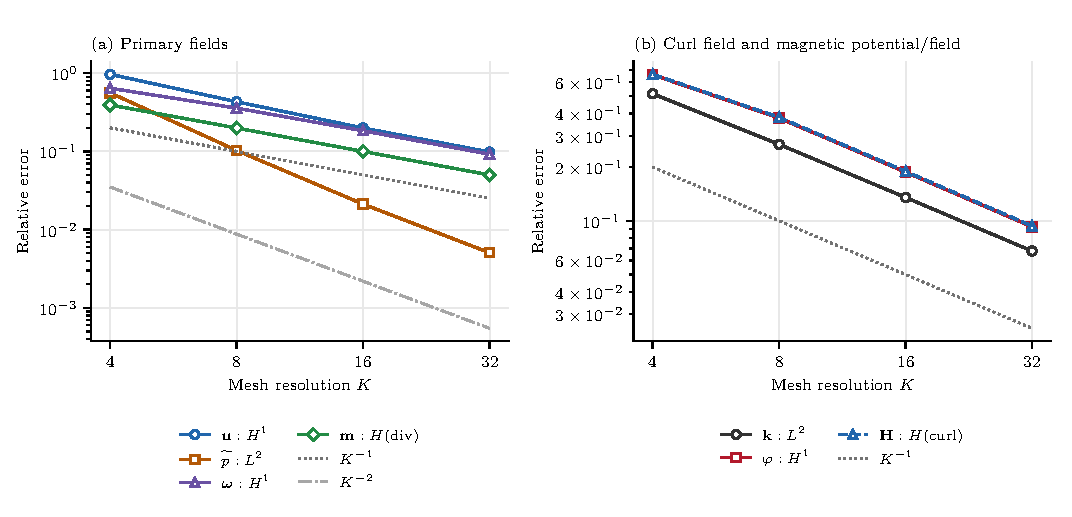
\includegraphics[width=\textwidth]{figures/first_order_errors.pdf}
\caption{Relative errors for the first-order discretization under joint
refinement with $\dt=1/K$.
(a) Velocity, modified pressure, angular velocity, and magnetization.
(b) Auxiliary curl field, magnetic potential, and magnetic field.
The horizontal coordinate is the mesh resolution $K=4,8,16,32$, so
refinement proceeds from left to right. Reference lines proportional
to $K^{-1}$ and $K^{-2}$ indicate first- and second-order decay with
mesh refinement, not independently measured temporal orders.}
\label{fig:first-order-convergence-rates}
\end{figure}

\FloatBarrier




%
%In this subsection, we provide numerical examples to verify the performance of the first-order scheme \eqref{eq:FHD-weak-fdis-1}. The numerical experiments are performed by using the fenics package \cite{Barattafenics}. In the following numerical examples, we take $\Omega = (0,1)^3$ and use $K \times K \times K$ uniform tetrahedral meshes with $K = 4,~8,~16,~32$. In the first example, we take the temporal step size as $\dt = h/\sqrt{3} = 1/K$.
%\begin{example}[Convergence order test]
%The exact solution, $(\bs u, p,\bs\omega,\bs m,\bs H)$, of the FHD model \eqref{eq:FHD} with $T = 2$ is given by
%\begin{align*}
%\bs u(x,y,z,t) & = e^{-t}[\sin(\pi y),\sin(\pi z),\sin(\pi x)]^\intercal, \\
%p(x,y,z,t) & = 120 x^2yz - 40 y^3 z - 40 y z^3,\\
%\bs\omega(x,y,z,t) & = e^{-t}[(x^2-x)(y^2-y)(z^2-z),0,0]^\intercal, \\
%\bs m(x,y,z,t) & = e^{-t}[\sin(\pi x)\sin(\pi y)\sin(\pi z),0,0]^\intercal,\\
%\bs H(x,y,z,t) & = 2000 e^{-t}
%\begin{pmatrix}
%(2x-1)(x^2-2)(y^2-y)^2(z^2-z)^2 \\
%(x^2-x)^2(2y-1)(y^2-y)(z^2-z)^2 \\
%(x^2-x)^2(y^2-y)^2(2z-1)(z^2-z)
%\end{pmatrix}.
%\end{align*}
%The parameters $\rho$, $\kappa$, $\eta$, $\zeta$, $\mu_0$, $\sigma$, $\eta^\prime$, $\lambda^\prime$, $\tau$ and $\chi_0$ are all chosen as $1$. Numerical results of the relative errors of the discrete solutions at $T = 2$ are list in \Cref{tab:first-order-errors}.
%\end{example}









%\begin{table}[htbp]
%\centering
%\caption{Errors and convergence rates for $\bs u$, $\tilde p$, $\bs\omega$, and $\bs m$.}
%\label{tab:first-order-errors-1}
%\renewcommand{\arraystretch}{1.15}
%\setlength{\tabcolsep}{4pt}
%\begin{tabular}{c|cc|cc|cc|cc}
%\hline
%$K$
%& $\|\bs u-\bs u_h\|_{H^1}$ & rate
%& $\|\tilde p-\tilde p_h\|_{L^2}$ & rate
%& $\|\bs\omega-\bs\omega_h\|_{H^1}$ & rate
%& $\|\bs m-\bs m_h\|_{H(\div)}$ & rate
%\\
%\hline
%4
%& $4.211325\mathrm{e}{-1}$ & -
%& $6.186498\mathrm{e}{-2}$ & -
%& $7.332370\mathrm{e}{-1}$ & -
%& $3.920085\mathrm{e}{-1}$ & -
%\\
%8
%& $1.437624\mathrm{e}{-1}$ & 1.551
%& $1.402318\mathrm{e}{-2}$ & 2.141
%& $3.127998\mathrm{e}{-1}$ & 1.229
%& $2.031512\mathrm{e}{-1}$ & 0.948
%\\
%16
%& $5.836239\mathrm{e}{-2}$ & 1.301
%& $3.418190\mathrm{e}{-3}$ & 2.037
%& $1.373081\mathrm{e}{-1}$ & 1.188
%& $1.024982\mathrm{e}{-1}$ & 0.987
%\\
%32
%& $2.715137\mathrm{e}{-2}$ & 1.104
%& $8.521882\mathrm{e}{-4}$ & 2.004
%& $6.530348\mathrm{e}{-2}$ & 1.072
%& $5.135994\mathrm{e}{-2}$ & 0.997
%\\
%\hline
%\end{tabular}
%\end{table}
%
%\begin{table}[htbp]
%\centering
%\caption{Errors and convergence rates for $\bs z$, $\bs k$, $\varphi$, and $\bs H$.}
%\label{tab:first-order-errors-2}
%\renewcommand{\arraystretch}{1.15}
%\setlength{\tabcolsep}{3.2pt}
%\resizebox{\textwidth}{!}{
%\begin{tabular}{c|cc|cc|cc|cc|cc}
%\hline
%$K$
%& $\|\bs z-\bs z_h\|_{H(\curl)}$ & rate
%& $\|\bs k-\bs k_h\|_{L^2}$ & rate
%& $\|\bs k-\bs k_h\|_{H(\curl)}$ & rate
%& $\|\varphi-\varphi_h\|_{H^1}$ & rate
%& $\|\bs H-\bs H_h\|_{H(\curl)}$ & rate
%\\
%\hline
%4
%& $5.254543\mathrm{e}{-1}$ & -
%& $5.048427\mathrm{e}{-1}$ & -
%& $5.438302\mathrm{e}{-1}$ & -
%& $6.296105\mathrm{e}{-1}$ & -
%& $6.325359\mathrm{e}{-1}$ & -
%\\
%8
%& $3.017882\mathrm{e}{-1}$ & 0.800
%& $2.618431\mathrm{e}{-1}$ & 0.947
%& $2.893750\mathrm{e}{-1}$ & 0.910
%& $3.392851\mathrm{e}{-1}$ & 0.892
%& $3.425366\mathrm{e}{-1}$ & 0.885
%\\
%16
%& $1.670097\mathrm{e}{-1}$ & 0.854
%& $1.321682\mathrm{e}{-1}$ & 0.986
%& $1.471292\mathrm{e}{-1}$ & 0.976
%& $1.697876\mathrm{e}{-1}$ & 0.999
%& $1.718949\mathrm{e}{-1}$ & 0.995
%\\
%32
%& $1.005726\mathrm{e}{-1}$ & 0.732
%& $6.624292\mathrm{e}{-2}$ & 0.997
%& $7.386648\mathrm{e}{-2}$ & 0.994
%& $8.473499\mathrm{e}{-2}$ & 1.003
%& $8.586550\mathrm{e}{-2}$ & 1.001
%\\
%\hline
%\end{tabular}}
%\end{table}
%
%
%\begin{table}[htbp]
%\centering
%\caption{Discrete curl-free property of the magnetic field.}
%\label{tab:curl-free-H}
%\begin{tabular}{c|c}
%\hline
%$K$ & $\|\curl\bs H_h\|_{L^\infty}$ \\
%\hline
%4  & $1.282776\mathrm{e}{-15}$ \\
%8  & $6.037851\mathrm{e}{-15}$ \\
%16 & $1.540932\mathrm{e}{-14}$ \\
%32 & $3.584284\mathrm{e}{-14}$ \\
%\hline
%\end{tabular}
%\end{table}

\section{Second-Order Scheme}

This section presents the construction of a second-order discrete scheme for the ferrohydrodynamic equations. We employ a modified Crank-Nicolson method for time discretization and adopt the finite element exterior calculus framework for spatial discretization.

\subsection{Time discretization}
In this subsection, we develop a second-order accurate time discretization for the ferrohydrodynamic equations. Building upon the abstract formulation, the scheme is designed to achieve higher temporal accuracy while preserving the intrinsic energy stability of the continuous problem.


\begin{algorithm}[H]
\caption{Second Order Scheme}\label{sch:2}
\begin{algorithmic}
%\begin{sch}[Second Order]\label{sch:2}
\STATE Given $\mathcal X^{n-1} \in \mathbb V$, find $\mathcal X^{n} \in \mathbb V$ and $\tilde p^n \in W$ such that
\begin{equation}\label{eq:FHD-semi-2}
\left\{
\begin{aligned}
\mathtt D(\delta_{t}\mathcal X^{n},\mathcal Y) + \mathtt A(\bar{\mathcal X}^{n-1/2},\mathcal Y) + \mathtt B(\hat{\mathcal X}^{n-1},\bar{\mathcal X}^{n-1/2},\mathcal Y) + \mathtt C(\mathcal Y,\bar{\tilde p}^n) & = (\mathtt f(\cdot,t_{n-1/2}),\mathcal Y) &&\forall~\mathcal Y \in \mathbb V, \\
\mathtt C(\bar{\mathcal X}^{n-1/2},q) & = 0 &&\forall~q \in W,
\end{aligned}
\right.
\end{equation}
with initial condition
\[
\mathcal X^{0} = \mathcal X_{0}.
\]
%\end{sch}
\end{algorithmic}
\end{algorithm}

\begin{remark}
In \cref{sch:2}, the solution at the first time level is computed using the fully nonlinear scheme to ensure consistency with the original problem and to provide an accurate starting value. For all subsequent time steps, a linearized implicit scheme is employed, in which the first argument of the trilinear form $\mathtt B(\cdot,\cdot,\cdot)$ is treated explicitly. This strategy reduces computational cost while preserving stability and the overall second-order temporal accuracy of the method.
\end{remark}

Similar to the analysis of \cref{sch:1}, we obtain the following existence and uniqueness result for the semi-discrete scheme \cref{sch:2}.

\begin{theorem}\label{the:existence-1}
For any $2 \le n \le N$, given $\mathcal X^{n-1} \in \mathbb V$ and $\mathcal X^{n-2} \in \mathbb V$, the semi-discrete scheme \cref{sch:2} admits a unique solution $(\mathcal X^n,\tilde p^n) \in \mathbb V \times W$ at each time step.
\end{theorem}

To investigate the stability of the scheme, we derive discrete energy estimates. By selecting appropriate test functions and exploiting the structural properties of the formulation, we obtain bounds that reflect the dissipative nature of the system.

\begin{theorem}[Energy estimate for \cref{sch:2}]\label{the:ener-semi-2}
Given $\mathcal X^{n-1} \in \mathbb V$ for $1 \leq n \leq N$, let $(\mathcal X^n,\tilde p^n) \in \mathbb V \times W$ be the unique solution of \cref{sch:2}. Then the following energy estimate holds:
\begin{equation}
\left(\max_{0 \leq n \leq N}\|\mathcal X^n\|_{\mathtt D}^2 + 2\dt \sum_{n = 1}^N \|\bar{\mathcal X}^{n-1/2}\|_{\mathtt A}^2\right)^{1/2}
\leq \|\mathcal X^0\|_{\mathtt D} + 2\dt \sum_{n = 1}^N\|\mathtt f(\cdot,t_{n-1/2})\|_{\mathtt D^{-1}}.
\end{equation}
\end{theorem}

\begin{proof}
The second equation of \eqref{eq:FHD-semi-2} implies that $\bar{\mathcal X}^{n-1/2} \in \mathfrak K$. Taking $\mathcal Y = \bar{\mathcal X}^{n-1/2} \in \mathfrak K \subset \mathbb V$ as a test function in the first equation of \eqref{eq:FHD-semi-2}, we obtain
\[
\|\mathcal X^n\|_{\mathtt D}^2 - \|\mathcal X^{n-1}\|_{\mathtt D}^2 + 2\dt\|\bar{\mathcal X}^{n-1/2}\|_{\mathtt A}^2
= 2\dt(\mathtt f(\cdot,t_{n-1/2}),\bar{\mathcal X}^{n-1/2}).
\]
Applying the Cauchy–Schwarz inequality yields
\[
2\dt(\mathtt f(\cdot,t_{n-1/2}),\bar{\mathcal X}^{n-1/2})
\leq \dt\|\mathtt f(\cdot,t_{n-1/2})\|_{\mathtt D^{-1}} \big(\|\mathcal X^n\|_{\mathtt D} + \|\mathcal X^{n-1}\|_{\mathtt D}\big).
\]
Hence,
\[
\|\mathcal X^n\|_{\mathtt D}^2 - \|\mathcal X^{n-1}\|_{\mathtt D}^2 + 2\dt\|\bar{\mathcal X}^{n-1/2}\|_{\mathtt A}^2
\leq \dt \|\mathtt f(\cdot,t_{n-1/2})\|_{\mathtt D^{-1}} \big(\|\mathcal X^n\|_{\mathtt D} + \|\mathcal X^{n-1}\|_{\mathtt D}\big).
\]

Summing from $n = 1$ to $L$ for any $1 \leq L \leq N$, we obtain
\[
\|\mathcal X^L\|_{\mathtt D}^2 + 2\dt\sum_{n = 1}^L\|\bar{\mathcal X}^{n-1/2}\|_{\mathtt A}^2
\leq \|\mathcal X^0\|_{\mathtt D}^2
+ \dt\sum_{n=1}^L\|\mathtt f(\cdot,t_{n-1/2})\|_{\mathtt D^{-1}} \big(\|\mathcal X^n\|_{\mathtt D} + \|\mathcal X^{n-1}\|_{\mathtt D}\big).
\]
Taking the maximum over $0 \leq n \leq N$ and using the arbitrariness of $L$, we deduce
\[
\max_{0 \leq n \leq N} \|\mathcal X^n\|_{\mathtt D}^2
+ 2\dt\sum_{n = 1}^N\|\bar{\mathcal X}^{n-1/2}\|_{\mathtt A}^2
\leq \|\mathcal X^0\|_{\mathtt D}^2
+ 2\dt\sum_{n = 1}^N\|\mathtt f(\cdot,t_{n-1/2})\|_{\mathtt D^{-1}}
\max_{0 \leq n \leq N} \|\mathcal X^n\|_{\mathtt D}.
\]
The desired estimate then follows from Lemma~\ref{lem:ieq-bas}.
\end{proof}
\begin{remark}
It follows from the proof of \cref{the:ener-semi-2} that, in the absence of the external field (i.e., $\bs H_e = 0$), the scheme \cref{sch:2} preserves the total energy in the sense that
\[
\|\mathcal X^L\|_{\mathtt D}^2 + 2\dt\sum_{n = 1}^L\|\bar{\mathcal X}^{n-1/2}\|_{\mathtt A}^2 = \|\mathcal X^0\|_{\mathtt D}^2\qquad\qquad\text{for any } 1\leq L \leq N.
\]
\end{remark}


In what follows, we focus on the error analysis of \cref{sch:2}. Analogously to the analysis for \cref{sch:1}, we begin by rewriting the weak formulation \eqref{eq:FHD-eq} at the intermediate time level $t_{n-1/2}$ ($1 \le n \le N$) in an equivalent form:
\begin{equation}\label{eq:sch2-tn}
\left\{
\begin{aligned}
&\mathtt D(\delta_t \mathcal X(\cdot,t_n),\mathcal Y) + \mathtt A(\bar{\mathcal X}(\cdot,t_{n-1/2}),\mathcal Y) + \mathtt B(\mathcal X(\cdot,t_{n-1/2}),\mathcal X(\cdot,t_{n-1/2}),\mathcal Y)  + \mathtt C(\mathcal Y,\bar{\tilde p}(\cdot,t_{n-1/2})) \\
&\qquad\qquad\qquad\quad = (\mathtt f(\cdot,t_{n-1/2}),\mathcal Y) + R_1(\mathcal Y) + R_2(\mathcal Y) + R_3(\mathcal Y), 
\qquad \forall~\mathcal Y \in \mathbb V,\\
& \mathtt C(\bar{\mathcal X}(\cdot,t_{n-1/2}),q) = 0,
\qquad \forall~q \in W,
\end{aligned}
\right.
\end{equation}
where
\[
\begin{aligned}
R_1(\mathcal Y) &:= \mathtt D\big(\delta_t\mathcal X(\cdot,t_n) - \partial_t\mathcal X(\cdot,t_{n-1/2}),\mathcal Y\big),\\
R_2(\mathcal Y) &:= \mathtt A\big(\bar{\mathcal X}(\cdot,t_{n-1/2}) - \mathcal X(\cdot,t_{n-1/2}),\mathcal Y\big),\\
R_3(\mathcal Y) &:= \mathtt C\big(\mathcal Y,\bar{\tilde p}(\cdot,t_{n-1/2}) - \tilde p(\cdot,t_{n-1/2})\big).
\end{aligned}
\]

Let $\mathtt e^n = \mathcal X(\cdot,t_n) - \mathcal X^n$ and $e_p^n = \tilde p(\cdot,t_n) - \tilde p^n$. We are now in a position to derive the corresponding error estimates.

\begin{theorem}[Error estimates for \cref{sch:2}]\label{the:err-semi2}
Let $(\mathcal X,\tilde p):(0,T]\to \mathbb V \times W$ be the solution of the continuous weak formulation \eqref{eq:FHD-eq}, and let $\{(\mathcal X^n,\tilde p^n)\}_{n=1}^N \subset \mathbb V \times W$ be the unique solution of the semi-discrete scheme \cref{sch:2}. Then the following error estimates hold:
\begin{align}\label{eq:err-sch2-1}
&\max_{1\le n\le N} \|\mathcal X(\cdot,t_n) - \mathcal X^n\|_{\mathtt D}^2 
+ \dt\sum_{n = 1}^N \|\bar{\mathcal X}(\cdot,t_{n-1/2}) - \bar{\mathcal X}^{n-1/2}\|_{\mathtt A}^2\notag \\
& \qquad \leq C\dt^4 \int_{0}^{T} \Big(\|\partial_{ttt}\mathcal X(\cdot,s)\|_{\mathtt D}^2 + \|\partial_{ttt}\mathcal X(\cdot,s)\|_{\mathtt A}^2 + \|\partial_{tt}\mathcal X(\cdot,s)\|_{\mathtt A}^2\Big)\,\dd s,\\
\label{eq:err-semi-sch2-2}
& \max_{1\le n \le N} \|\mathcal X(\cdot,t_n) - \mathcal X^n\|_{\mathtt A}^2  
+ \dt\sum_{n=1}^N \|\delta_t(\mathcal X(\cdot,t_n) - \mathcal X^n)\|_{\mathtt D}^2 
\notag\\
&\qquad 
\leq C\dt^4 \int_0^T \Big(\|\partial_{ttt}\mathcal X(\cdot,s)\|_{\mathtt D}^2 + \|\partial_{tt}\mathcal X(\cdot,s)\|_{\mathbb W}^2 + \|\partial_{ttt}\mathcal X(\cdot,s)\|_{\mathtt A}^2 + \|\partial_{ttt}\mathcal X(\cdot,s)\|_{\mathbb W}^2\Big)\,\dd s,\\
\label{eq:err-semi-sch2-3} 
& \dt\sum_{n = 1}^N\|\bar{\tilde p}(\cdot,t_{n-1/2}) - \bar{\tilde p}^{n-1/2}\|^2 \notag\\
&\qquad \leq C\dt^4 \int_0^T \Big(\|\partial_{ttt}\mathcal X(\cdot,s)\|_{\mathtt D}^2 + \|\partial_{tt}\mathcal X(\cdot,s)\|_{\mathbb W}^2 + \|\partial_{ttt}\mathcal X(\cdot,s)\|_{\mathtt A}^2 + \|\partial_{ttt}\mathcal X(\cdot,s)\|_{\mathbb W}^2  + \|\partial_{tt}\tilde p(\cdot,s)\|^2 + \|\partial_{ttt}\tilde p(\cdot,s)\|^2\Big)\,\dd s.
\end{align}
\end{theorem}
\begin{proof}


Subtracting \cref{sch:2} from \eqref{eq:sch2-tn}, we obtain
\begin{equation}\label{eq:err-semi-pr-2}
\left\{
\begin{aligned}
\mathtt D(\delta_t \mathtt e^n,\mathcal Y) + \mathtt A(\bar{\mathtt e}^{n-1/2},\mathcal Y) + \mathtt C(\mathcal Y,\bar{e}_p^{n-1/2})&  = R_1(\mathcal Y) + R_2(\mathcal Y)+ R_3(\mathcal Y)  \\
&\quad - [\mathtt B(\mathcal X(\cdot,t_{n-1/2}),\mathcal X(\cdot,t_{n-1/2}),\mathcal Y) - \mathtt B(\hat{\mathcal X}^{n-1},\bar{\mathcal X}^{n-1/2},\mathcal Y)] & & \forall~\mathcal Y \in \mathbb V,\\
\mathtt C(\bar{\mathtt e}^{n-1/2},q) & = 0
%\mathtt C(\bar{\mathcal X}(\cdot,t_{n-1/2})- \mathcal X(\cdot,t_{n-1/2}),q) 
& & \forall~q \in W.
\end{aligned}
\right.
\end{equation}

Taking the test functions $\mathcal Y = \bar{\mathtt e}^{n-1/2} \in \mathbb V$ and $q = \bar{e}_p^{n-1/2}\in W$ in \cref{eq:err-semi-pr-2}, we obtain
\[
\begin{aligned}
\|\mathtt e^n\|_{\mathtt D}^2 - \|\mathtt e^{n-1}\|_{\mathtt D}^2 + 2\dt\|\bar{\mathtt e}^{n-1/2}\|_{\mathtt A}^2 &= 2\dt R_1(\bar{\mathtt e}^{n-1/2}) + 2\dt R_2(\bar{\mathtt e}^{n-1/2}) 
%+ 2\dt R_3(\bar{\mathtt e}^{n-1/2}) - 2\dt\mathtt C(\bar{\mathcal X}(\cdot,t_{n-1/2}) - \mathcal X(\cdot,t_{n-1/2}),\bar{e}_p^{n-1/2}) 
\\
& \quad -2\dt [\mathtt B(\mathcal X(\cdot,t_{n-1/2}),\mathcal X(\cdot,t_{n-1/2}),\bar{\mathtt e}^{n-1/2}) - \mathtt B(\hat{\mathcal X}^{n-1},\bar{\mathcal X}^{n-1/2},\bar{\mathtt e}^{n-1/2})] \\
&\leq 2\dt\|\delta_t\mathcal X(\cdot,t_n) - \partial_t\mathcal X(\cdot,t_{n-1/2})\|_{\mathtt D}\|\bar{\mathtt e}^{n-1/2}\|_{\mathtt D} +2\dt\|\bar{\mathcal X}(\cdot,t_{n-1/2}) - \mathcal X(\cdot,t_{n-1/2})\|_{\mathtt A}\|\bar{\mathtt e}^{n-1/2}\|_{\mathtt A} \\
%&\quad + 2\dt\|\bar{\mathtt e}^{n-1/2}\|_{\mathbb V}\|\bar{\tilde p}(\cdot,t_{n-1/2}) - \tilde p(\cdot,t_{n-1/2})\| + 2\dt \|\bar{\mathcal X}(\cdot,t_{n-1/2}) - \mathcal X(\cdot,t_{n-1/2})\|_{\mathbb V} \|\bar{e}_p^{n-1/2}\| \\
&\quad + C\dt \|\mathcal X(\cdot,t_{n-1/2})\|_{\mathbb V}\|\mathcal X(\cdot,t_{n-1/2}) - \bar{\mathcal X}(\cdot,t_{n-1/2})\|_{\mathbb V}\|\bar{\mathtt e}^{n-1/2}\|_{\mathbb V} \\
&\quad + C\dt \|\bar{\mathcal X}(\cdot,t_{n-1/2})\|_{\mathbb V}\|\bar{\mathtt e}^{n-1/2}\|_{\mathtt A} \|\hat{\mathcal X}(\cdot,t_{n-1}) - \mathcal X(\cdot,t_{n-1/2})\|_{\mathtt A} \\
&\quad + C\dt \|\bar{\mathcal X}(\cdot,t_{n-1/2})\|_{\mathbb W} \|\bar{\mathtt e}^{n-1/2}\|_{\mathbb V}\|\hat{\mathtt e}^{n-1}\|_{\mathtt D}.
\end{aligned}
\]
For any quantity $J(t)$, using the identities:
\[
\begin{aligned}
J(t_n) - J(t_{n-1}) - \dt \partial_t J(t_{n-1/2}) & = -\frac{1}{2}\int_{t_{n-1}}^{t_n} (s- t_{n-1})(t_n - s)\partial_{ttt}J(s)\dd s + \frac{\dt}{2}\int_{t_{n-1/2}}^{t_n} \int_{s-\dt/2}^s \partial_{ttt}J(l)\dd l\dd s,\\
\bar{J}(t_{n-1/2}) - J(t_{n-1/2}) & = \frac{1}{2}\int_{t_{n-1}}^{t_{n-1/2}} (t_{n-1} - s) \int_s^{s+\dt/2}\partial_{ttt}J(l)\dd l\dd s + \frac{\dt}{4} \int_{t_{n-1}}^{t_{n-1/2}} \partial_{tt}J(s+\dt/2)\dd s,\\
\hat J(t_{n-1}) - J(t_{n-1/2}) & = \left\{
\begin{aligned}
& -\frac{1}{2}\int_{t_{n-1}}^{t_n} \int_{s-\dt}^{s-\dt/2}\partial_{tt} J(l)\dd l\dd s -\frac{1}{2}\int_{t_{n-1}}^{t_{n-1/2}}\int_{s-\dt/2}^{s}\partial_{tt} J(l)\dd l\dd s, &\quad \text{for } n\geq 2,\\
&\frac{1}{2}\int_{t_{0}}^{t_{1/2}} (t_{0} - s) \int_s^{s+\dt/2}\partial_{ttt}J(l)\dd l\dd s + \frac{\dt}{4} \int_{t_{0}}^{t_{1/2}} \partial_{tt}J(s+\dt/2)\dd s,&\quad\text{for } n=1,
\end{aligned}
\right.
\end{aligned}
\]
we have
\[
\begin{aligned}
\|\mathtt e^n\|_{\mathtt D}^2 - \|\mathtt e^{n-1}\|_{\mathtt D}^2 &+ 2\dt\|\bar{\mathtt e}^{n-1/2}\|_{\mathtt A}^2  \leq C\dt^{5/2}\|\bar{\mathtt e}^{n-1/2}\|_{\mathtt D} \left(\int_{t_{n-1}}^{t_n} \|\partial_{ttt}\mathcal X(\cdot,s)\|_{\mathtt D}^2 \dd s \right)^{1/2} + C\dt^{7/2}\|\bar{\mathtt e}^{n-1/2}\|_{\mathtt A} \left( \int_{t_{n-1}}^{t_n} \|\partial_{ttt}\mathcal X(\cdot,s)\|_{\mathtt A}^2 \dd s\right)^{1/2} \\
& + C\dt^{5/2}\|\bar{\mathtt e}^{n-1/2}\|_{\mathtt A} \left( \int_{t_{n-1}}^{t_n} \|\partial_{tt}\mathcal X(\cdot,s)\|_{\mathtt A}^2 \dd s\right)^{1/2} 
%+ C\dt^{7/2}\|\bar{\mathtt e}^{n-1/2}\|_{\mathtt A} \left( \int_{t_{n-1}}^{t_n} \|\partial_{ttt}\tilde p(\cdot,s)\|^2 \dd s\right)^{1/2} \\
%& + \dt^{5/2} \|\bar{\mathtt e}^{n-1/2}\|_{\mathtt A} \left( \int_{t_{n-1}}^{t_n} \|\partial_{tt}\tilde p(\cdot,s)\|^2 \dd s\right)^{1/2} +C\dt^{7/2} \|\bar e_p^{n-1/2}\| \left( \int_{t_{n-1}}^{t_n} \|\partial_{ttt}\mathcal X(\cdot,s)\|_{\mathtt A}^2 \dd s\right)^{1/2} \\
%& + C\dt^{5/2}\|\bar e_p^{n-1/2}\| \left( \int_{t_{n-1}}^{t_n} \|\partial_{tt}\mathcal X(\cdot,s)\|_{\mathtt A}^2 \dd s\right)^{1/2} 
+ C\dt^{7/2} \|\mathcal X(\cdot,t_{n-1/2})\|_{\mathbb V} \|\bar{\mathtt e}^{n-1/2}\|_{\mathtt A} \left( \int_{t_{n-1}}^{t_n} \|\partial_{ttt}\mathcal X(\cdot,s)\|_{\mathtt A}^2 \dd s\right)^{1/2} \\
& + C\dt^{5/2} \|\mathcal X(\cdot,t_{n-1})\|_{\mathbb V} \|\bar{\mathtt e}^{n-1/2}\|_{\mathtt A} \left( \int_{t_{n-1}}^{t_n} \|\partial_{tt}\mathcal X(\cdot,s)\|_{\mathtt A}^2 \dd s\right)^{1/2}+ C\dt \|\bar{\mathcal X}(\cdot,t_{n-1/2})\|_{\mathbb W} \|\bar{\mathtt e}^{n-1/2}\|_{\mathtt A}\|\hat{\mathtt e}^{n-1}\|_{\mathtt D} \\
&+\left\{ 
\begin{aligned}
& C\dt^{5/2}\|\bar{\mathcal X}(\cdot,t_{n-1/2})\|_{\mathbb V}\|\bar{\mathtt e}^{n-1/2}\|_{\mathtt A}  \left( \int_{t_{n-2}}^{t_n} \|\partial_{tt}\mathcal X(\cdot,s)\|_{\mathtt A}^2 \dd s\right)^{1/2} &\quad\text{for } n \geq 2,  \\
&C \|\bar{\mathcal X}(\cdot,t_{n-1/2})\|_{\mathbb V} \|\bar{\mathtt e}^{1/2}\|_{\mathtt A} \left(\dt^7 \int_{t_{0}}^{t_1} \|\partial_{ttt}\mathcal X(\cdot,s)\|_{\mathtt A}^2 \dd s + \dt^5 \int_{t_0}^{t_1} \|\partial_{tt}\mathcal X(\cdot,s)\|_{\mathtt A}^2\dd s\right)^{1/2} &\quad\text{for } n = 1.
\end{aligned}
\right.
\end{aligned}
\]
Using 
%the estimate of $\|\bar e_p^{n-1/2}\|$ and 
the Young's inequality, we get
\[
\begin{aligned}
\|\mathtt e^n\|_{\mathtt D}^2 - \|\mathtt e^{n-1}\|_{\mathtt D}^2  +2 \dt \|\bar{\mathtt e}^{n-1/2}\|_{\mathtt A}^2 \leq &  \dt \|\bar{\mathtt e}^{n-1/2}\|_{\mathtt A}^ 2 + C\dt^4 \int_{t_{n-1}}^{t_n} \left(\|\partial_{ttt}\mathcal X(\cdot,s)\|_{\mathtt D}^2 + \|\partial_{ttt}\mathcal X(\cdot,s)\|_{\mathtt A}^2 + \|\partial_{tt}\mathcal X(\cdot,s)\|_{\mathtt A}^2 
%+ \|\partial_{ttt}\tilde p(\cdot,s)\|^2 + \|\partial_{tt}\tilde p(\cdot,s)\|^2
 \right)\dd s\\
& + C\dt \|\bar{\mathcal X}(\cdot,t_{n-1/2})\|_{\mathbb W}^2 \|\hat{\mathtt e}^{n-1}\|_{\mathtt D}^2.
% + 
%\left\{
%\begin{aligned}
%& C\dt^{5/2}\|\bar{\mathcal X}(\cdot,t_{n-1/2})\|_{\mathbb V} (\|\mathtt e^n\|_{\mathtt D} + \|\mathtt e^{n-1}\|_{\mathtt D})\left( \int_{t_{n-2}}^{t_n} \|\partial_{tt}\mathcal X(\cdot,s)\|_{\mathbb W}^2 \dd s\right)^{1/2} &\quad\text{for } n\geq 2,\\
%& C\dt^{3/2} \|\bar{\mathcal X}(\cdot,t_{n-1/2})\|_{\mathbb V} (\|\mathtt e^n\|_{\mathtt D} + \|\mathtt e^{n-1}\|_{\mathtt D})\left( \int_{t_{n-1}}^{t_n} \|\partial_{t}\mathcal X(\cdot,s)\|_{\mathbb W}^2 \dd s\right)^{1/2} & \quad\text{for } n = 1. 
%\end{aligned}
%\right.
%\\
%& + C\dt^{3/2} (\|\mathtt e^n\|_{\mathtt D} + \|\mathtt e^{n-1}\|_{\mathtt D}) \left( \int_{t_{n-1}}^{t_n} \|\partial_{tt}\mathcal X(\cdot,s)\|_{\mathtt A}^2 \dd s\right)^{1/2}.
\end{aligned}
\]
Summing the above inequality from $n = 1$ to $L$ for any $1\leq L\leq N$ and using the regularity assumption the the weak solution, we have
\[
\begin{aligned}
\|\mathtt e^L\|_{\mathtt D}^2 & + \dt\sum\limits_{n = 1}^L \|\bar{\mathtt e}^{n-1/2}\|_{\mathtt A}^2  \leq C\dt^4 \int_{0}^{T} \left(\|\partial_{ttt}\mathcal X(\cdot,s)\|_{\mathtt D}^2 + \|\partial_{ttt}\mathcal X(\cdot,s)\|_{\mathtt A}^2 + \|\partial_{tt}\mathcal X(\cdot,s)\|_{\mathtt A}^2 
%+ \|\partial_{ttt}\tilde p(\cdot,s)\|^2 + \|\partial_{tt}\tilde p(\cdot,s)\|^2 
\right)\dd s + C\dt\sum\limits_{n = 1}^L\|\mathtt e^n\|_{\mathtt D}^2.
\end{aligned}
\]
Then, the discrete Gr\"onwall inequality implies \cref{eq:err-sch2-1}.

Taking the test function $\mathcal Y = \delta_t\mathtt e^n \in \mathbb V$ in the first equation of \cref{eq:err-semi-pr-2},  we obtain
\[
\begin{aligned}
\|\mathtt e^n\|_{\mathtt A}^2 - \|\mathtt e^{n-1}\|_{\mathtt A}^2 &+ 2\dt \|\delta_t\mathtt e^n\|_{\mathtt D}^2  =2\dt R_1(\delta_t\mathtt e^n) +2\dt R_2(\delta_t\mathtt e^n) - 2\dt[\mathtt B(\mathcal X(\cdot,t_{n-1/2}),\mathcal X(\cdot,t_{n-1/2}),\delta_t\mathtt e^n) - \mathtt B(\hat{\mathcal X}^{n-1},\bar{\mathcal X}^{n-1/2},\delta_t\mathtt e^n)] \\
& \leq C\dt^{5/2}\|\delta_t\mathtt e^n\|_{\mathtt D} \left(\int_{t_{n-1}}^{t_n} \|\partial_{ttt}\mathcal X(\cdot,s)\|_{\mathtt D}^2\dd s \right)^{1/2} + C\dt^{7/2}\|\delta_t\mathtt e^n\|_{\mathtt A}\left(\int_{t_{n-1}}^{t_n} \|\partial_{ttt}\mathcal X(\cdot,s)\|_{\mathtt A}^2\dd s \right)^{1/2} \\
&\quad + C\dt^{5/2}\|\delta_t\mathtt e^n\|_{\mathtt A} \left(\int_{t_{n-1}}^{t_n} \|\partial_{tt}\mathcal X(\cdot,s)\|_{\mathtt A}^2\dd s \right)^{1/2} + C\dt^{5/2}\|\mathcal X(\cdot,t_{n-1/2})\|_{\mathbb W}\|\delta_t\mathtt e^n\|_{\mathtt D} \left(\int_{t_{n-1}}^{t_n} \|\partial_{ttt}\mathcal X(\cdot,s)\|_{\mathtt A}^2\dd s \right)^{1/2} \\
&\quad + C\dt \|\mathcal X(\cdot,t_{n-1/2})\|_{\mathbb W} \|\delta_t\mathtt e^n\|_{\mathtt D} \|\bar{\mathtt e}^{n-1/2}\|_{\mathtt A} + C\dt\|\hat{\mathtt e}^{n-1}\|_{\mathtt A}\|\bar{\mathcal X}^{n-1/2}\|_{\mathbb W}\|\delta_t\mathtt e^n\|_{\mathtt D} \\
& \quad 
+\left\{ 
\begin{aligned}
& C\dt^{5/2}\|\bar{\mathcal X}^{n-1/2}\|_{\mathbb V}\|\delta_t\mathtt e^{n}\|_{\mathtt D}  \left( \int_{t_{n-2}}^{t_n} \|\partial_{tt}\mathcal X(\cdot,s)\|_{\mathbb W}^2 \dd s\right)^{1/2} &\quad\text{for } n \geq 2,  \\
&C \|\bar{\mathcal X}^{n-1/2}\|_{\mathbb V} \|\delta_t\mathtt e^{1}\|_{\mathtt D} \left(\dt^7 \int_{t_{0}}^{t_1} \|\partial_{ttt}\mathcal X(\cdot,s)\|_{\mathbb W}^2 \dd s + \dt^5 \int_{t_0}^{t_1} \|\partial_{tt}\mathcal X(\cdot,s)\|_{\mathbb W}^2\dd s\right)^{1/2} &\quad\text{for } n = 1.
\end{aligned}
\right.
%
%
%+ C\dt^{5/2}\|\bar{\mathcal X}^{n-1/2}\|_{\mathtt A}\|\delta_t\mathtt e^n\|_{\mathtt D}\left(\int_{t_{n-2}}^{t_n} \|\partial_{tt}\mathcal X(\cdot,s)\|_{\mathbb W}^2\dd s \right)^{1/2} 
\end{aligned}
\]
The Young's inequality implies
\[
\begin{aligned}
\|\mathtt e^n\|_{\mathtt A}^2 - \|\mathtt e^{n-1}\|_{\mathtt A}^2 & + 2\dt\|\delta_t\mathtt e^n\|_{\mathtt D}^2  \leq \dt\|\delta_t\mathtt e^n\|_{\mathtt D}^2 + \dt^4 \int_{t_{n-1}}^{t_n}(\|\partial_{ttt}\mathcal X(\cdot,s)\|_{\mathtt D}^2 + \|\partial_{tt}\mathcal X(\cdot,s)\|_{\mathbb W}^2 +\|\partial_{ttt}\mathcal X(\cdot,s)\|_{\mathtt A}^2+\|\partial_{ttt}\mathcal X(\cdot,s)\|_{\mathbb W}^2)\dd s \\
& 
%+ C\dt^{5/2}(\|\mathtt e^n\|_{\mathtt A}+\|\mathtt e^{n-1}\|_{\mathtt A})\left(\int_{t_{n-1}}^{t_n} \|\partial_{ttt}\mathcal X(\cdot,s)\|_{\mathtt A}^2\dd s \right)^{1/2}   
+ C\dt^{3/2}(\|\mathtt e^n\|_{\mathtt A} +\|\mathtt e^{n-1}\|_{\mathtt A})\left(\int_{t_{n-1}}^{t_n} (\|\partial_{tt}\mathcal X(\cdot,s)\|_{\mathtt A}^2 + \|\partial_{ttt}\mathcal X(\cdot,s)\|_{\mathtt A}^2\dd s \right)^{1/2} + C\dt \|\bar{\mathcal X}^{n-1/2}\|_{\mathbb W}^{2}\|\hat{\mathtt e}^{n-1}\|_{\mathtt A}^2\\&
+ C\dt\|\mathcal X(\cdot,t_{n-1/2})\|_{\mathbb W}^2(\|\mathtt e^n\|_{\mathtt A}^2 +\|\mathtt e^{n-1}\|_{\mathtt A}^2)  .
\end{aligned}
\]
%For $n = 1$, we obtain
%\[
%\begin{aligned}
%\|\mathtt e^1\|_{\mathtt A}^2  &+ 2\dt \|\delta_t\mathtt e^1\|_{\mathtt D}^2  
%%=2\dt R_1(\delta_t\mathtt e^n) +2\dt R_2(\delta_t\mathtt e^n) - 2\dt[\mathtt B(\mathcal X(\cdot,t_{n-1/2}),\mathcal X(\cdot,t_{n-1/2}),\delta_t\mathtt e^n) - \mathtt B(\hat{\mathcal X}^{n-1},\bar{\mathcal X}^{n-1/2},\delta_t\mathtt e^n)] \\
% \leq C\dt^{5/2}\|\delta_t\mathtt e^1\|_{\mathtt D} \left(\int_{t_{0}}^{t_1} \|\partial_{ttt}\mathcal X(\cdot,s)\|_{\mathtt D}^2\dd s \right)^{1/2} + C\dt^{7/2}\|\delta_t\mathtt e^1\|_{\mathtt A}\left(\int_{t_{0}}^{t_1} \|\partial_{ttt}\mathcal X(\cdot,s)\|_{\mathtt A}^2\dd s \right)^{1/2} \\
%&\quad + C\dt^{5/2}\|\delta_t\mathtt e^1\|_{\mathtt A} \left(\int_{t_{0}}^{t_1} \|\partial_{tt}\mathcal X(\cdot,s)\|_{\mathtt A}^2\dd s \right)^{1/2} + C\dt^{5/2}\|\mathcal X(\cdot,t_{1/2})\|_{\mathbb W}\|\delta_t\mathtt e^1\|_{\mathtt D} \left(\int_{t_{0}}^{t_1} \|\partial_{ttt}\mathcal X(\cdot,s)\|_{\mathtt A}^2\dd s \right)^{1/2} \\
%&\quad + C\dt \|\mathcal X(\cdot,t_{1/2})\|_{\mathbb W} \|\delta_t\mathtt e^1\|_{\mathtt D} \|\bar{\mathtt e}^{1/2}\|_{\mathtt A} + C\dt^{3/2}\|\bar{\mathcal X}^{1/2}\|_{\mathtt A}\|\delta_t\mathtt e^1\|_{\mathtt A}\left(\int_{t_{0}}^{t_1} \|\partial_{t}\mathcal X(\cdot,s)\|_{\mathtt A}^2\dd s \right)^{1/2} \\
%&\quad + C\dt\|\hat{\mathtt e}^{0}\|_{\mathtt A}\|\bar{\mathcal X}^{1/2}\|_{\mathbb W}\|\delta_t\mathtt e^1\|_{\mathtt D} \\
%& \leq \dt\|\delta_t\mathtt e^1\|_{\mathtt D}^2 + C\dt^4\int_{t_0}^{t_1} (\|\partial_{ttt}\mathcal X(\cdot,s)\|_{\mathtt D}^2 +  \|\partial_{ttt}\mathcal X(\cdot,s)\|_{\mathtt A}^2 )\dd s + C\dt^{3/2} \|\mathtt e^1\|_{\mathtt A} \left(\int_{t_0}^{t_1} (\|\partial_{tt}\mathcal X(\cdot,s)\|_{\mathtt A}^2 + \|\partial_{tt}\mathcal X(\cdot,s)\|_{\mathtt A}^2)\dd s \right)^{1/2} \\
%&\quad + C\dt (\|\mathcal X(\cdot,t_{1/2})\|_{\mathcal Z}^2 + \|\bar{\mathcal X}^{1/2}\|_{\mathbb W}^2)\|\mathtt e^1\|_{\mathtt A}^2 + C\dt \|\bar{\mathcal X}^{1/2}\|_{\mathtt A} \|\partial_t\mathcal X\|_{L^\infty(t_0,t_1,\mathbb V)}\|\mathtt e^1\|_{\mathtt A},
%\end{aligned}
%\]
%
Summing the above equation from $n = 1$ to $L$ for any $1\leq L\leq N$, we have
\[
\|\mathtt e^L\|_{\mathtt A}^2 + \dt\sum\limits_{n = 1}^L\|\delta_t\mathtt e^n\|_{\mathtt D}^2 \leq \dt^4 \int_0^T(\|\partial_{ttt}\mathcal X(\cdot,s)\|_{\mathtt D}^2 + \|\partial_{tt}\mathcal X(\cdot,s)\|_{\mathbb W}^2 +\|\partial_{ttt}\mathcal X(\cdot,s)\|_{\mathtt A}^2+\|\partial_{ttt}\mathcal X(\cdot,s)\|_{\mathbb W}^2)\dd s + C\dt\sum\limits_{n=1}^L \|\mathtt e^n\|_{\mathtt A}^2.
\]
The discrete Gr\"onwall inequality implies \cref{eq:err-semi-sch2-2}.

The inf-sup condition \eqref{eq:C-inf-sup} and the first equation of \eqref{eq:err-semi-pr-2} imply
\[
\begin{aligned}
\|\bar{e}_p^{n-1/2} \| & \lesssim \sup\limits_{\mathcal Y \in \mathbb V\setminus\{0\}}\frac{\mathtt C(\mathcal Y,\bar{e}_p^{n-1/2})}{\|\mathcal Y\|_{\mathbb V}} \\
& =\sup\limits_{\mathcal Y \in \mathbb V\setminus\{0\}}\frac{-\mathtt D(\delta_t\mathtt e^n,\mathcal Y) - \mathtt A(\bar{\mathtt e}^{n-1/2},\mathcal Y) + R_1(\mathcal Y) + R_2(\mathcal Y) + R_3(\mathcal Y) -[\mathtt B(\mathcal X(\cdot,t_{n-1/2}),\mathcal X(\cdot,t_{n-1/2}),\mathcal Y) - \mathtt B(\mathcal X^{n-1},\bar{\mathcal X}^{n-1/2},\mathcal Y)] }{\|\mathcal Y\|_{\mathbb V}} \\
& \lesssim \|\delta_t \mathtt e^n\|_{\mathtt D} + \|\bar{\mathtt e}^{n-1/2}\|_{\mathtt A} + \|\delta_t\mathcal X(\cdot,t_{n-1/2}) - \mathcal X(\cdot,t_{n-1/2})\|_{\mathtt D} + \|\bar{\mathcal X}(\cdot,t_{n-1/2}) - \mathcal X(\cdot,t_{n-1/2})\|_{\mathtt A} + \|\bar{\tilde p}(\cdot,t_{n-1/2}) - \tilde p(\cdot,t_{n-1/2})\|\\
& \quad + \|\mathcal X(\cdot,t_{n-1/2})\|_{\mathbb V}\|\mathcal X(\cdot,t_{n-1/2}) - \bar{\mathcal X}(\cdot,t_{n-1/2})\|_{\mathbb V} + \|\bar{\mathcal X}(\cdot,t_{n-1/2})\|_{\mathbb V}\|\mathcal X(\cdot,t_{n-1/2}) - \mathcal X(\cdot,t_{n-1})\|_{\mathbb V} \\
&\quad + \|\bar{\mathcal X}(\cdot,t_{n-1/2})\|_{\mathbb W}\|\mathtt e^{n-1}\|_{\mathtt D} + \|\mathcal X^{n-1}\|_{\mathbb V} \|\bar{\mathtt e}^{n-1/2}\|_{\mathtt A}.
\end{aligned}
\]
Then, \cref{eq:err-semi-sch2-3} follows by using \eqref{eq:err-sch2-1} and \eqref{eq:err-semi-sch2-2}.
\end{proof}





\subsection{Spatial discretization}
%Let $\mathcal T_h$ be a quasi-uniform and shape-regular triangulation of $\Omega$ with mesh size $h >0$.
%We now introduce the conforming finite element spaces employed for the spatial discretization. These include $H^1$-, $H(\curl)$- and $H(\div)$- conforming finite element spaces defined on the triangulation $\mathcal T_h$. For any element $K \in \mathcal T_h$ and any integer $ l\geq 0$, let $\mathbb P_l(K)$ denote the space of polynomials defined on $K$ with total degree at most $l$.
%%
%We introduce the following conforming finite element spaces for the spatial discretization:
%\begin{itemize}
%	\item $\bs S_h = (S_h)^3 \subset \bs S$, where $S_h$ is a continuous piecewise polynomial space \cite{Arnoldmini1984}, with the local space defined for any $K \in \mathcal T_h$ as: $S_h|_K = \mathbb P_1(K) + B_K$, where $B_K$ denotes the bubble function space spanned by the quartic bubble function:
%	$$
%	\qquad\quad B_K = \hbox{span}\left\{\prod\limits_{i = 1}^4 \lambda_i^K:~\lambda_i^K \ (i=1,\cdots,4)\text{ is the barycentric coordinates of element }K\right\}.
%	$$
%	\item $L_h \subset H^1(\Omega)\cap W$ is the standard continuous linear finite element space \cite{Ciarlet1978}.
%	\item $\bs\Sigma_h = (\Sigma_h)^3 \subset \bs S$, where $\Sigma_h$ is the continuous piecewise linear finite element space \cite{Ciarlet1978}.
%	\item $\bs U_h \subset \bs U$, the lowest order edge-element space ($NE_0$) \cite{Nedelec1980,Nedelec1986}, with the local containment property $(\mathbb P_0(K))^3 \subset \bs U_h|_K$ for all $K \in \mathcal T_h$.
%	\item $\bs V_h \subset \bs V$, the lowest order face-element space ($RT_0$) \cite{Raviart;Thomas1977}, satisfying $(\mathbb P_0(K))^3 \subset \bs V_h|_K$.
%	\item $W_h\subset W$, the space of piecewise constant functions~\cite{Ciarlet1978}.
%\end{itemize}
%The chosen finite element spaces satisfy two fundamental properties essential for numerical stability:
%\begin{itemize}
%\item[(1) ]The inf-sup condition \cite{Arnoldmini1984}:
%\begin{equation}
%\label{eq:inf-sup} \sup\limits_{\bs v_h \in \bs S_h\setminus\{0\}}\frac{(q_h,\div\bs v_h)}{\|\bs v_h\|_1} \gtrsim \|q_h\|\qquad\qquad\forall~q_h \in L_h. 
%\end{equation}
%\item[(2) ]The commutative exact sequence \cite{Hiptmair2002}:
%\begin{equation}\label{eq:exact_sq}
%\begin{CD}
%H_0^1@>{\grad}>> \bs U @>{\curl}>> \bs V @>{\div}>> W \\
%@VV \pi_h V @ VV \pi ^{c}_h V  @VV \pi ^d_h V @ VV Q_h V \\\
%\Sigma_{h} @>{\grad}>> \bs U_{h} @>{\curl}>>  \bs V_{h} @>{\div}>> W_{h}
%\end{CD}
%\end{equation}
%Here $\pi_h:~H_0^1(\Omega)\to \Sigma_h$, $\pi_h^c:\bs U \to \bs U_h$ and $\pi_h^d:\bs V \to \bs V_h$ are the canonical interpolation operators, while $Q_h: W \to W_h$ denotes the $L^2$-orthogonal projection.
%\end{itemize}
%
%We define three discrete weak operators,
%$$
%\div_h:\bs U_h \to\Sigma_h,\quad\curl_h:\bs V_h \to \bs U_h,\quad \grad_h:W_h \to \bs V_h,
%$$
%as the adjoint operators of $-\grad$, $\curl$ and $-\div$, respectively. More precisely: 
%\begin{itemize}
%\item For any $\bs u_h \in \bs U_h$, the discrete divergence $\div_h \bs u_h \in \Sigma_h$ is characterized by:
%\begin{equation}
%\label{eq:div-h} (\div_h\bs u_h, s_h) := -(\bs v_h,\grad s_h) \qquad\forall~s_h \in \Sigma_h.
%\end{equation}
%\item For any $\bs v_h \in \bs V_h$, the discrete curl $\curl_h\bs v_h \in \bs U_h$ is characterized by:
%\begin{equation}
%\label{eq:curl-h} (\curl_h\bs v_h,\bs u_h) := (\bs v_h,\curl\bs u_h)\qquad\forall~\bs u_h \in \bs U_h.
%\end{equation}
%\item For any $w_h \in W_h$, the discrete gradient $\grad_hw_h \in \bs V_h$ is characterized by:
%\begin{equation}
%\label{eq:grad-h} (\grad_h w_h,\bs v_h) := -(w_h,\div\bs v_h)\qquad\forall~\bs v_h \in \bs V_h.
%\end{equation}
%\end{itemize}
%These definitions yield the following cochain complex, which is exact for the specific finite element spaces we have selected:
%\begin{equation}\label{eq:exact-seq-re}
%\begin{CD}
%0@<{}<<\Sigma_h @<{\div_h}<< \bs U_h @<{\curl_h}<< \bs V_h @<{\grad_h}<< W_h@<{}<<0
%\end{CD}
%\end{equation} 
%
%Introduce the discrete analogues of the kernel spaces for the differential operators:
%$$
%\mathfrak Z_{h}^{c} = \bs U_{h} \cap \ker(\curl),\quad\text{and}\quad \mathfrak Z_{h}^{d} = \bs V_{h}\cap \ker(\div),
%$$
%and for the discrete weak operators:
%$$
%\mathfrak K_{h}^{c} = \bs U_{h}\cap \ker(\div_{h}),\quad\text{and}\quad \mathfrak K_{h}^{d} = \bs V_{h} \cap \ker(\curl_{h}).
%$$
%These spaces admit the following Hodge decomposition \cite{Arnold;Falk;Winther2006,Arnold;Falk;Winther2010}:
%\begin{align}
%\label{eq:hodge-dis-1}
%\bs U_{h} & = \mathfrak Z_{h}^{c} \oplus ^{\bot}\mathfrak K_{h}^{c}= \grad\Sigma_{h} \oplus^{\bot} \div_{h}\bs U_{h},\\ 
%\label{eq:hodge-dis-2}
%\bs V_{h} &= \mathfrak Z_{h}^{d} \oplus^{\bot}\mathfrak K_{h}^{d} = \curl\bs U_{h} \oplus^{\bot} \grad_{h}W_{h}.
%\end{align}
%%
%We also define the discrete space of solenoidal vector fields:
%$$
%\mathfrak K_h^s = \{ \bs v_h \in \bs S_h:~(\div\bs v_h,q_h) = 0\quad\forall~q_h \in L_h\}.
%$$

%We define the Hilbert space 
%$$
%\mathbb V_h^2 := \bs S_h^2 \times \bs\Sigma_h^2 \times \bs V_h^2 \times \Sigma_h^2 \subset \mathbb V.
%$$
For any $\mathcal X_h = (\bs u_h,\bs\omega_h,\bs m_h,\varphi_h)^\intercal \in \mathbb V_h^2$, $\mathcal Y_h = (\bs v_h,\bs s_h,\bs F_h,\psi_h)^\intercal \in \mathbb V_h^2$ and $\mathcal Z_h = (\bs \epsilon_h,\bs \sigma_h,\bs A_h,\phi_h)^\intercal \in \mathbb V_h^2$, we define the discrete bilinear form $\mathtt A_h^2:\mathbb V_h^2\times \mathbb V_h^2 \to \mathbb R$ as:
\begin{align*}
\mathtt A_h^2(\mathcal X_h,\mathcal Y_h) := & \eta(\nabla\bs u_h,\nabla\bs v_h) +\eta^\prime(\nabla\bs\omega_h,\nabla\bs s_h) + (\eta^\prime +\lambda^\prime)(\div\bs\omega_h,\div\bs s_h) + \sigma(\curl_h^2\bs m_h,\curl_h^2\bs F_h) + \sigma(\div\bs m_h,\div\bs F_h)\\
&+ \frac{1}{\tau}(\bs m_h,\bs F_h) + \frac{\mu_0(1+\chi_0)+\chi_0}{\tau}(\nabla\varphi_h,\nabla\psi_h) +\sigma\mu_0(\Delta_h^2\varphi_h,\Delta_h^2\psi_h) + \zeta(\curl\bs u_h,\curl\bs v_h) -2\zeta(\bs \omega_h,\curl\bs v_h) \\
& -2\zeta(\curl\bs u_h,\bs s_h) + 4\zeta(\bs\omega_h,\bs s_h),
\end{align*}
and define the discrete trilinear form $\mathtt B_h^2:~\mathbb V_h^2 \times \mathbb V_h^2 \times \mathbb V_h^2 \to \mathbb R$ as:
\begin{align*}
\mathtt B_h^2(\mathcal Z_h,\mathcal X_h,\mathcal Y_h) := & \rho b(\bs\epsilon_h,\bs u_h,\bs v_h) + \rho\kappa b(\bs\epsilon_h,\bs\omega_h,\bs s_h) - c(\bs\epsilon_h,\bs m_h,\bs F_h) - \frac{1}{2}(\bs m_h\times \curl\bs\epsilon_h,\bs F_h) -(\bs\sigma_h \times\bs m_h,\bs F_h)\\
& + \mu_0[(\nabla\varphi_h,\bs v_h\div\bs A_h) - (\nabla\psi_h,\bs u_h\div\bs A_h)] +\frac{\mu_0}{2}[\bs u_h \times\curl_h^2\bs A_h,\nabla\psi_h) - (\bs v_h \times\curl_h^2\bs A_h,\nabla\varphi_h)] \\
&+ \frac{\mu_0}{2}[(\bs A_h \times\curl\bs u_h,\nabla\psi_h) - (\bs A_h\times\curl\bs v_h,\nabla\varphi_h)]  + \mu_0[(\bs\omega_h \times \bs A_h,\nabla\psi_h) - (\bs s_h\times \bs A_h,\nabla\varphi_h)] \\
&+ \frac{\chi_0}{\tau}[(\bs m_h,\nabla\psi_h) - (\bs F_h,\nabla\varphi_h)] + \frac{1}{2}[(\bs\epsilon_h \times\bs F_h,\curl_h^2\bs m_h) - (\bs\epsilon_h \times\bs m_h,\curl_h^2\bs F_h)]\\
&  + \frac{\mu_0}{2}\bigl[(\Delta_h^2\psi_h,\bs u_h\cdot\bs A_h) - (\Delta_h^2\varphi_h,\bs v_h\cdot\bs A_h) \bigr].
\end{align*}
Obviously, $\mathtt B_h^2$ is skew-symmetric with respect to the second and third variables, i.e., 
\begin{equation}
\mathtt B_h^2(\mathcal Z_h,\mathcal X_h,\mathcal Y_h) = -\mathtt B_h^2(\mathcal Z_h,\mathcal Y_h,\mathcal X_h)\qquad\forall~\mathcal X_h,~\mathcal Z_h,~\mathcal Y_h \in \mathbb V_h^2.
\end{equation}

For any $ 1\leq n \leq N$, the second order abstract formulation of the fully discrete schemes of \eqref{eq:FHD} read as: 
%\begin{sch}[First order]
% Given $\mathcal X_h^{n-1} \in \mathbb V$, find $\mathcal X_h^{n} \in \mathbb V$ and $\tilde p_h^n\in L_h$, such that
%\begin{equation}\label{eq:FHD-full-1}
%\left\{
%\begin{array}{rll}
%\mathtt D(\delta_{t}\mathcal X_h^{n},\mathcal Y_h) + \mathtt A(\mathcal X_h^{n},\mathcal Y_h) + \mathtt B_h(\mathcal X_h^{n-1},\mathcal X_h^{n},\mathcal Y_h) + \mathtt C(\mathcal Y_h,\tilde p_h^n) & = (\mathtt f(\cdot,t_n),\mathcal Y_h) & \forall~\mathcal Y_h \in \mathbb V_h, \\
%\mathtt C(\mathcal X_h^n,q_h) & = 0 &\forall~q_h\in L_h,
%\end{array}
%\right.
%\end{equation}
%with initial value
%$$
%\mathcal X_h^{0}(\cdot) = \mathcal I_h\mathcal X_{0}(\cdot).
%$$
%\end{sch}
%%
\begin{algorithm}[H]
\caption{Second Order Scheme (fully discretization)}\label{sch:2-f-d}
\begin{algorithmic}
%\begin{sch}[Second order]
\STATE Given $\mathcal X_h^{n-1} \in \mathbb V_h^2$, find $\mathcal X_h^{n} \in \mathbb V_h^2$ and $\tilde p_h^n\in L_h$, such that
\begin{equation}\label{eq:FHD-ful-2}
\left\{
\begin{array}{rll}
\mathtt D(\delta_{t}\mathcal X_h^{n},\mathcal Y_h) + \mathtt A_h^2(\bar{\mathcal X}_h^{n-1/2},\mathcal Y_h) + \mathtt B_h^2(\hat{\mathcal X}_h^{n-1},\bar{\mathcal X}_h^{n-1/2},\mathcal Y_h) + \mathtt C(\mathcal Y_h,\bar{\tilde p}_h^{n-1/2}) & = (\mathtt f(\cdot,t_{n-1/2}),\mathcal Y_h) & \forall~\mathcal Y_h \in \mathbb V_h^2, \\
\mathtt C(\overline{\mathcal X}_h^{n-1/2},q_h) & = 0 &\forall~q_h\in L_h,
\end{array}
\right.
\end{equation}
with initial value
$$
\mathcal X_h^{0}(\cdot) = \mathcal I_h^2\mathcal X_{0}(\cdot).
$$
%\end{sch}
\end{algorithmic}
\end{algorithm}

Similar to the analysis of \cref{sch:1,sch:2}, we obtain the following existence and uniqueness result for the fully discrete scheme \cref{sch:2-f-d}.

\begin{theorem}\label{the:existence-2-f-d}
For any $2 \le n \le N$, given $\mathcal X_h^{n-1} \in \mathbb V_h^2$ and $\mathcal X_h^{n-2} \in \mathbb V_h^2$, the fully discrete scheme \cref{sch:2-f-d} admits a unique solution $(\mathcal X_h^n,\tilde p_h^n) \in \mathbb V_h^2 \times L_h$ at each time step.
\end{theorem}

%To investigate the stability of the scheme, we derive discrete energy estimates. By selecting appropriate test functions and exploiting the structural properties of the formulation, we obtain bounds that reflect the dissipative nature of the system.

\begin{theorem}[Energy estimate for \cref{sch:2-f-d}]\label{the:ener-f-2}
Given $\mathcal X_h^{n-1} \in \mathbb V_h^2$ for $1 \leq n \leq N$, let $(\mathcal X_h^n,\tilde p_h^n) \in \mathbb V_h^2 \times L_h$ be the unique solution of \cref{sch:2-f-d}. Then the following energy estimate holds:
\begin{equation}
\left(\max_{0 \leq n \leq N}\|\mathcal X_h^n\|_{\mathtt D}^2 + 2\dt \sum_{n = 1}^N \|\bar{\mathcal X_h}^{n-1/2}\|_{\mathtt A}^2\right)^{1/2}
\leq \|\mathcal X_h^0\|_{\mathtt D} + 2\dt \sum_{n = 1}^N\|\mathtt f(\cdot,t_{n-1/2})\|_{\mathtt D^{-1}}.
\end{equation}
\end{theorem}

At each time level \(t_n\), for any discrete quantity \(\bs v_h\), we use the notation
\[
\bar{\bs v}_h:=\bar{\bs v}_h^{n-1/2}, \qquad \hat{\bs v}_h^- := \hat{\bs v}_h^{n-1},\qquad 
\bs v_h:=\bs v_h^{n}, \qquad
\delta_t\bs v_h:=\delta_t\bs v_h^{n}.
\]
With this convention, the fully discrete scheme \eqref{eq:FHD-ful-2} in \cref{sch:2-f-d} can be equivalently rewritten in the following computable form.
Find 
\[
\begin{aligned}
& \bs u_h\in \bs S_h^2, & & \tilde p_h \in L_h, & & \bs\omega_h\in \bs\Sigma_h^2, & & \bs m_h\in \bs V_h^2,\\
& \bs z_h\in \bs U_h^2, & & \bs k_h \in\bs U_h^2, && \varphi_h \in \Sigma_h^2, && \vartheta_h \in \Sigma_h^2, & & \varpi_h \in \Sigma_h^2,
\end{aligned}
\] 
such that, for all
\[
\begin{aligned}
& \bs v_h\in \bs S_h^2, & & \tilde q_h \in L_h, & &\bs s_h\in \bs\Sigma_h^2, & & \bs F_h\in \bs V_h^2,\\
& \bs \lambda_h\in \bs U_h^2, & & \bs \theta_h \in\bs U_h^2, & & \psi_h \in \Sigma_h^2, &&  \varsigma_h \in \Sigma_h^2, & & \gamma_h \in \Sigma_h^2,
\end{aligned}
\] 
it holds
\begin{equation}
\label{eq:FHD-weak-fdis-2}
\left\{ \begin{array}{rl}
\rho(\delta_t\bs u_h,\bs v_h) + \rho b(\hat{\bs u}_h^-,\bar{\bs u}_h,\bs v_h) + \eta(\nabla\bar{\bs u}_h,\nabla\bs v_h) + \zeta (\curl\bar{\bs u}_h,\curl\bs v_h) - 2\zeta(\bar{\bs\omega}_h,\curl\bs v_h)
- (\bar{\tilde p}_h,\div\bs v_h) & \\
+\frac{\mu_0}{2} (\bar\vartheta_h,\hat{\bs m}_h^-\cdot\bs v_h) + \frac{\mu_0}{2} (\nabla\bar{\varphi}_h \div\hat{\bs m}_h^-,\bs v_h) - \frac{\mu_0}{2}(\bs v_h \times \hat{\bs k}_h^-,\nabla\bar{\varphi}_h) 
- \frac{\mu_0}{2}(\hat{\bs m}_h^-\times \curl\bs v_h,\nabla\bar\varphi_h) 
 &= 0, \\
(\div\bar{\bs u}_h,q_h) & = 0, \\
\rho\kappa(\delta_t\bs\omega_h,\bs s_h) + \eta^\prime(\nabla\bar{\bs\omega}_h,\nabla\bs s_h) + (\eta^\prime + \lambda^\prime)(\div\bar{\bs\omega}_h,\div\bs s_h) + 4\zeta(\bar{\bs \omega}_h,\bs s_h)
+ \rho\kappa b(\hat{\bs u}_h^-,\bar{\bs\omega}_h,\bs s_h)  & \\-\mu_0(\hat{\bs m}_h^-\times \nabla\bar\varphi_h,\bs s_h)
%
- 2\zeta(\curl\bar{\bs u}_h,\bs s_h) &  = 0,\\
(\delta_t\bs m_h,\bs F_h)  + \frac{1}{\tau}(\bar{\bs m}_h,\bs F_h) +\sigma(\curl\bar{\bs k}_h,\bs F_h) + \sigma(\div\bar{\bs m}_h,\div\bs F_h)- c(\hat{\bs u}_h^-,\bar{\bs m}_h,\bs F_h) 
-\frac{1}{2}(\bar{\bs m}_h\times\curl\hat{\bs u}_h^-,\bs F_h) &\\
- \frac{1}{2}(\hat{\bs u}_h^- \times \bar{\bs k}_h,\bs F_h)  
- \frac{1}{2}(\curl\bar{\bs z}_h,\bs F_h) 
- (\hat{\bs\omega}_h^-\times \bar{\bs m}_h,\bs F_h) 
-\frac{\chi_0}{\tau}(\nabla\bar\varphi_h,\bs F_h) & = 0, \\
(\bs z_h,\bs\lambda_h) - (\hat{\bs u}_h^- \times \bar{\bs m}_h,\bs\lambda_h) & = 0,\\
(\bs k_h,\bs \theta_h) - (\bs m_h,\curl\bs\theta_h) & = 0,\\
\mu_0(\delta_t\nabla\varphi_h,\nabla\psi_h) + \frac{\mu_0(1+\chi_0)+\chi_0}{\tau}(\nabla\bar\varphi_h,\nabla\psi_h) + \sigma\mu_0(\nabla\bar\vartheta_h,\nabla\psi_h) +\mu_0(\bar{\bs\omega}_h\times \hat{\bs m}_h^-,\nabla\psi_h) +\frac{\chi_0}{\tau}(\bar{\bs m}_h ,\nabla\psi_h) & \\
-\frac{\mu_0}{2}(\nabla\bar\varpi_h,\nabla\psi_h) -\frac{\mu_0}{2}(\bar{\bs u}_h\div\hat{\bs m}_h^-,\nabla\psi_h) + \frac{\mu_0}{2}(\hat{\bs m}_h^-\times \curl\bar{\bs u}_h,\nabla\psi_h)
+\frac{\mu_0}{2}(\bar{\bs u}_h \times \hat{\bs k}_h^-,\nabla\psi_h) & \\
+ (\partial_t\bs H_e(t_{n-1/2},\nabla\psi_h) + \frac{\mu_0+\chi_0}{\tau\mu_0}(\bs H_e(t_n-1/2),\nabla\psi_h)+ \sigma(\grad\div\bs H_e(t_n-1/2),\nabla\psi_h)& = 0, \\
\sigma\mu_0(\bar\vartheta_h,\varsigma_h) -\sigma\mu_0 (\nabla\bar\varphi_h,\nabla\varsigma_h) & = 0,\\
(\bar\varpi_h,\gamma_h) - (\bar{\bs u}_h\cdot\hat{\bs m}_h^-,\gamma_h) & = 0.
\end{array}
\right.
\end{equation}
After solving \eqref{eq:FHD-weak-fdis-2}, we can obtain $\bs H_h \in \bs U_h^2$ by solving
\begin{equation}\label{eq:H-dis-f-1}
(\bs H_h,\bs \varepsilon_h) = (\nabla\varphi_h,\bs \varepsilon_h) \qquad\forall~\bs\varepsilon_h \in \bs U_h^2.
\end{equation}
Consequently, \(\bs H_h = \nabla\varphi_h$ and therefore $\curl\bs H_h = 0$ pointwise in $\Omega$.


\begin{remark}
When $n=1$, the fully discrete system \eqref{eq:FHD-weak-fdis-2} is
nonlinear. To solve the resulting nonlinear algebraic system, we employ
the quasi-Newton iteration developed in
\cite{WuXie2023a,WuXie2025}. For $2\le n\le N$, owing to the
extrapolation treatment of the nonlinear terms, the system
\eqref{eq:FHD-weak-fdis-2} becomes linear and has the same block
algebraic structure as the first-order scheme
\eqref{eq:FHD-weak-fdis-1}. Consequently, the linear systems arising at
these time levels can be solved efficiently by the exact Schur
complement decoupling solver presented in
\cref{alg:exact-schur-decoupling}.
\end{remark}

The fully discrete error analysis of the second-order scheme follows
essentially the same strategy as that of the first-order method. By
introducing suitable quasi-interpolation operators, the spatial
approximation errors can be treated in a standard manner, while the main
additional issue is the consistency error associated with the discrete
differential operators. Since no essentially new arguments are required,
we omit the technical details here for brevity and refer to the arXiv
version of this paper for the complete fully discrete error analysis.


\subsection{Numerical results}
\label{subsec:numerical-second-order}
We apply the second-order discretization to the same manufactured
solution, forcing, parameters, and meshes specified in
\Cref{subsec:revised-numerical-first}, retaining $T=2$ and $\dt=1/K$.
Velocity and angular velocity now use continuous piecewise quadratic
elements, pressure remains continuous piecewise linear, magnetization
uses RT1, and $\bs z,\bs k,\bs H$ use first-family Nedelec elements
one degree above the lowest order. The scalar fields
$\varphi,\vartheta,\varpi$ are continuous piecewise quadratic.
The corresponding RT and Nedelec Basix degree is two.

The first time step is solved by a Broyden quasi-Newton iteration with
relative tolerance $10^{-9}$ and a maximum of 12 iterations.
The accepted state is checked by reassembling the nonlinear midpoint
equations. Subsequent time steps use the prescribed extrapolated
coefficients and require one five-block linear solve per step.
The $\bs z_h$ and $\varpi_h$ slots represent the current midpoint-stage
projections; they are not averaged again with the preceding stage.

The primary fields are compared at $T$. The pressure slot represents
the averaged modified pressure, so its reference is
\[
\widetilde p_{\mathrm{ref}}^{N-1/2}
=\frac{\widetilde p(T)+\widetilde p(T-\dt)}{2},
\]
with the same zero-mean convention as above. This reference is not
identified with either the endpoint pressure or the analytic pressure
evaluated directly at the midpoint.

\Cref{tab:second-order-errors,fig:second-order-convergence} show that
the finest-grid rates for $\bs u,\widetilde p,\bs\omega,\bs m,
\varphi,\bs H$ are 2.166, 2.051, 1.981, 2.007, 1.968, and 1.968,
respectively. The $L^2$ error of $\bs k$ decreases approximately at
first order, with a finest-grid rate of 1.015; second-order convergence
is therefore not claimed for every auxiliary quantity.
The sampled curl diagnostic ranges from $7.30\times10^{-13}$ to
$6.96\times10^{-11}$. For $K=32$, all 64 steps reach $T=2$, and
the final full-system relative algebraic residual is
$2.08\times10^{-13}$.
These observations support the reported joint-refinement behavior.
Because the mesh and time step vary together and the primary exact
fields have linear temporal amplitudes, they do not constitute a
separate test of pure temporal accuracy or of energy stability.

\begin{table}[htbp]
\centering
\caption{Relative errors and observed rates for the second-order scheme, $T=2$ and $\dt=1/K$. $C_H$ is the sampled absolute curl diagnostic.}
\label{tab:second-order-errors}
\begingroup
\small
\setlength{\tabcolsep}{3.5pt}
\renewcommand{\arraystretch}{1.15}
\begin{tabular}{crrrrrrrr}
\toprule
\multicolumn{9}{c}{(a) Velocity, pressure, angular velocity, and magnetization}\\
\midrule
$K$ & \multicolumn{2}{c}{$\bs u$: $H^1$} & \multicolumn{2}{c}{$\widetilde p$: $L^2$} & \multicolumn{2}{c}{$\bs\omega$: $H^1$} & \multicolumn{2}{c}{$\bs m$: $H(\div)$}\\
 & Error & Rate & Error & Rate & Error & Rate & Error & Rate\\
\midrule
4 & $5.6873\!\times\!10^{-1}$ & -- & $4.2000\!\times\!10^{-1}$ & -- & $2.1381\!\times\!10^{-1}$ & -- & $1.1937\!\times\!10^{-1}$ & --\\
8 & $1.5090\!\times\!10^{-1}$ & 1.914 & $9.4815\!\times\!10^{-2}$ & 2.147 & $6.2017\!\times\!10^{-2}$ & 1.786 & $3.1613\!\times\!10^{-2}$ & 1.917\\
16 & $2.4805\!\times\!10^{-2}$ & 2.605 & $2.0872\!\times\!10^{-2}$ & 2.184 & $1.6320\!\times\!10^{-2}$ & 1.926 & $7.8383\!\times\!10^{-3}$ & 2.012\\
32 & $5.5259\!\times\!10^{-3}$ & 2.166 & $5.0382\!\times\!10^{-3}$ & 2.051 & $4.1345\!\times\!10^{-3}$ & 1.981 & $1.9494\!\times\!10^{-3}$ & 2.007\\
\bottomrule
\end{tabular}
\par\medskip
\begin{tabular}{crrrrrrr}
\toprule
\multicolumn{8}{c}{(b) Auxiliary curl field, potential, magnetic field, and curl diagnostic}\\
\midrule
$K$ & \multicolumn{2}{c}{$\bs k$: $L^2$} & \multicolumn{2}{c}{$\varphi$: $H^1$} & \multicolumn{2}{c}{$\bs H$: $H(\curl)$} & $C_H$\\
 & Error & Rate & Error & Rate & Error & Rate &\\
\midrule
4 & $2.1008\!\times\!10^{-1}$ & -- & $2.0119\!\times\!10^{-1}$ & -- & $2.0303\!\times\!10^{-1}$ & -- & $7.3001\!\times\!10^{-13}$\\
8 & $9.5804\!\times\!10^{-2}$ & 1.133 & $6.0098\!\times\!10^{-2}$ & 1.743 & $6.0718\!\times\!10^{-2}$ & 1.742 & $3.9064\!\times\!10^{-12}$\\
16 & $4.6084\!\times\!10^{-2}$ & 1.056 & $1.6119\!\times\!10^{-2}$ & 1.899 & $1.6289\!\times\!10^{-2}$ & 1.898 & $1.8492\!\times\!10^{-11}$\\
32 & $2.2804\!\times\!10^{-2}$ & 1.015 & $4.1189\!\times\!10^{-3}$ & 1.968 & $4.1627\!\times\!10^{-3}$ & 1.968 & $6.9611\!\times\!10^{-11}$\\
\bottomrule
\end{tabular}
\endgroup
\end{table}

\begin{figure}[htbp]
\centering
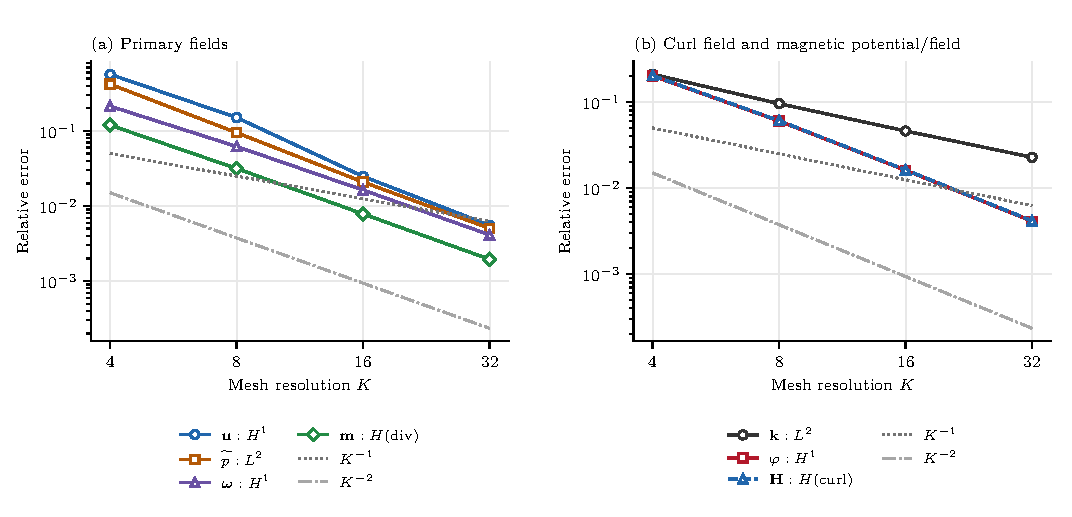
\includegraphics[width=\textwidth]{figures/second_order_errors.pdf}
\caption{Relative errors for the second-order discretization using the
same manufactured solution and $\dt=1/K$.
(a) Velocity, averaged modified pressure, angular velocity, and magnetization.
(b) Auxiliary curl field, magnetic potential, and magnetic field.
The horizontal coordinate is $K=4,8,16,32$, increasing from left to
right. Reference lines proportional to $K^{-1}$ and $K^{-2}$ distinguish
the nearly quadratic decay of the principal errors from the
approximately first-order $L^2$ decay for $\bs k$.}
\label{fig:second-order-convergence}
\end{figure}

\subsubsection{Second-order scheme}
\label{subsec:second-order-energy}
\Cref{fig:second-order-energy} shows monotone energy decay for all
three time steps, with initial energy approximately
$4.295033\times10^{-2}$.
\Cref{tab:second-order-energy} reports the final ratios and balance
diagnostics; the largest normalized balance defect is
$3.71\times10^{-11}$.
The coarsest time step produces slower late-time decay, which is
retained in the plot. Energy dissipation therefore should not be
interpreted as evidence that the temporal error is negligible.
Since the two schemes also use different spatial approximation
orders, these figures are separate stability tests rather than
a controlled comparison of temporal accuracy. The computations
provide numerical evidence of the discrete dissipation mechanism
at the tested step sizes, not a proof for arbitrary step sizes.

\begin{table}[htbp]
\centering
\caption{Second-order unforced energy test: $K=8$, $T=0.5$.}
\label{tab:second-order-energy}
\small
\begin{tabular}{crr}
\toprule
$\dt$ & $E_h(T)/E_h(0)$ & $\max_n\epsilon_{\rm bal}^n$\\
\midrule
$1/16$ & $1.1117\times10^{-4}$ & $3.71\times10^{-11}$\\
$1/32$ & $2.5984\times10^{-5}$ & $7.77\times10^{-13}$\\
$1/64$ & $1.0438\times10^{-5}$ & $2.67\times10^{-13}$\\
\bottomrule
\end{tabular}
\end{table}

\begin{figure}[htbp]
\centering
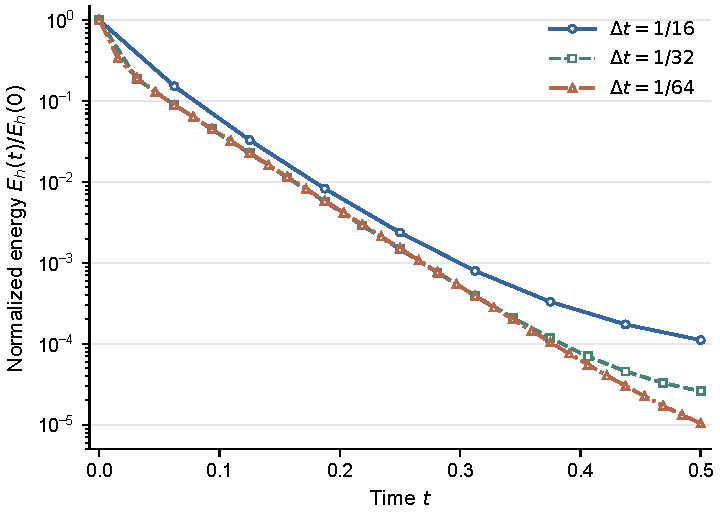
\includegraphics[width=0.70\textwidth]{figures/second_order_energy.pdf}
\caption{Normalized discrete energy for the second-order scheme in the
unforced relaxation test, $K=8$ and $T=0.5$.
The logarithmic vertical scale matches \Cref{fig:first-order-energy}.
Symbols represent all computed time levels without smoothing.
The same discrete initial state is used for all three time steps.}
\label{fig:second-order-energy}
\end{figure}
\FloatBarrier







%We introduce two projection-based quasi-interpolation operators 
%$
%I_h^c: \bs U \to \bs U_h$ and $I_h^d: \bs V \to \bs V_h$,
%whose detailed definitions can be found in \cite{Wu2020,WuXie2023}.  
%These quasi-interpolation operators satisfy the following properties; see \cite[Lemmas 3.3--3.5]{Wu2020} and \cite[Lemma 2.10]{WuXie2023}.
%\begin{lemma} \label{lem:Ih}
%The projection-based quasi-interpolation operators $I_h^c$ and $I_h^d$ satisfy the following properties:
%
%\begin{enumerate}
%\item For any $\bs u \in \bs U$ and $\bs v \in \bs V$, we have
%\begin{align*}
%& (I_h^c \bs u, \grad s_h) = (\bs u, \grad s_h), && \forall~ s_h \in \Sigma_h,\\
%& (I_h^d \bs v, \curl \bs \phi_h) = (\bs v, \curl \bs \phi_h), && \forall~ \bs \phi_h \in \bs U_h,\\
%& (\curl I_h^c \bs u, \curl \bs \psi_h) = (\curl \bs u, \curl \bs \psi_h), && \forall~ \bs \psi_h \in \bs U_h,\\
%& (\div I_h^d \bs v, \div \bs \phi_h) = (\div \bs v, \div \bs \phi_h), && \forall~ \bs \phi_h \in \bs V_h.
%\end{align*}
%
%\item For any $\bs u \in \bs U$ and $\bs v \in \bs V$, the following stability estimates hold:
%\[
%\|\curl I_h^c \bs u\| \leq \|\curl \bs u\|, \qquad
%\|\div I_h^d \bs v\| \leq \|\div \bs v\|.
%\]
%
%\item For any $\bs u \in H_0(\curl) \cap H(\div)$ and $\bs v \in H_0(\div) \cap H(\curl)$, we have
%\[
%\div_h I_h^c \bs u = Q_h^g \div \bs u, \qquad
%\curl_h I_h^d \bs v = Q_h^c \curl \bs v,
%\]
%where $Q_h^g : L^2(\Omega) \to \Sigma_h$ and $Q_h^c : \bs L^2(\Omega) \to \bs U_h$ are $L^2$-orthogonal projections. Consequently,
%\[
%\|\div_h I_h^c \bs u\| \leq \|\div \bs u\|, \qquad
%\|\curl_h I_h^d \bs v\| \leq \|\curl \bs v\|.
%\]
%
%\item For any $\bs u \in \bs U \cap H^{l+1}(\Omega)$ and $\bs v \in \bs V \cap H^{l+1}(\Omega)$ with $l \geq 0$, there holds
%\[
%\|\bs u - I_h^c \bs u\| \lesssim h^r \|\bs u\|_r, \quad
%\|\bs v - I_h^d \bs v\| \lesssim h^r \|\bs v\|_r, \qquad 1 \leq r \leq l+1.
%\]
%Moreover, if $\curl \bs u \in H^{l+1}(\Omega)$ and $\div \bs v \in H^{l+1}(\Omega)$, then
%\[
%\|\curl(I - I_h^c) \bs u\| \lesssim h^r \|\curl \bs u\|_r, \quad
%\|\div(I - I_h^d) \bs v\| \lesssim h^r \|\div \bs v\|_r, \qquad 1 \leq r \leq l+1.
%\]
%
%\item For any $\bs u \in L^\infty(\Omega) \cap \bs U$ and $\bs v \in L^\infty(\Omega) \cap \bs V$, there holds
%\[
%\|I_h^c \bs u\|_{L^\infty} \lesssim \|\bs u\|_{L^\infty}, \qquad
%\|I_h^d \bs v\|_{L^\infty} \lesssim \|\bs v\|_{L^\infty}.
%\]
%\end{enumerate}
%\end{lemma}



%\section{Abstract framework}\label{sec:abstrac}
%
%This section develops an abstract analytical framework for studying the regularity properties and numerical approximation of a class of nonlinear parabolic partial differential equations. We establish both semi-discrete and fully discrete formulations within this unified framework, and prove optimal-order error estimates for each discretization scheme in abstract operator-theoretic terms.
%
%
%\subsection{Abstract problem}
%Let $\Omega\subset \mathbb R^d$ ($d = 2,~3$) be a bounded simply connected convex domain with Lipschitz boundary $\partial\Omega$, and $T>0$ be the final time. We use $L^2(\Omega)$ to denote the space of all square integrable scalar or vector functions on $\Omega$, with the inner product $(\cdot,\cdot)$ and norm $\|\cdot\|$.
%Let $\mathbb V \subset L^2(\Omega)$ and $\mathbb W\subset L^2(\Omega)$ be two subspace of $L^2(\Omega)$ with inner-products $(\cdot,\cdot)_{\mathbb V}$ and $(\cdot,\cdot)_{\mathbb W}$, and the induced norms $\|\cdot\|_{\mathbb V}$ and $\|\cdot\|_{\mathbb W}$, respectively. We assume $\mathbb W\subset \mathbb V$ and $\|\mathcal Y\| \lesssim \|\mathcal Y\|_{\mathbb V}$ for all $\mathcal Y \in \mathbb V$ and $\|\mathcal Z\|_{\mathbb V} \lesssim \|\mathcal Z\|_{\mathbb W}$ for all $\mathcal Z \in \mathbb W$. 
%We define $\mathcal V:~\mathbb V \to \mathbb V$ as
%$$
%(\mathcal V\mathcal Y,\mathcal Z) = (\mathcal Y,\mathcal Z)_{\mathbb V}\qquad\forall~\mathcal Y,~\mathcal Z \in \mathbb V.
%$$
%The dual space of $\mathbb V$ is denoted as $\mathbb V^\prime$ and the duality pair is denoted as $\langle\cdot,\cdot\rangle$. The norm on the dual space $
%\mathbb V^{\prime}$ is defined by 
%$$\|\mathtt f \|_{\mathbb V^{\prime}} = \sup\limits_{\mathcal Y \in \mathbb V\setminus \{0\}}\frac{\langle \mathtt f,\mathcal Y\rangle}{\|\mathcal Y\|_{\mathbb V}}.$$
%The operator $\mathcal J:~\mathbb V^\prime\to \mathbb V$ is the Riesz operator, i.e., for any $\mathtt g \in \mathbb V^\prime$ and $\mathcal Y \in \mathbb V$, we have
%$$
%(\mathcal J\mathtt g,\mathcal Y)_{\mathbb V} = \langle \mathtt g,\mathcal Y\rangle\qquad\text{and}\qquad \|\mathcal J\mathtt g\|_{\mathbb V} = \|\mathtt g\|_{\mathbb V^\prime}.
%$$
%We define linear operator space $\mathcal L(\mathbb V,\mathbb V^\prime)$ as
%\begin{align*}
%\mathcal L(\mathbb V,\mathbb V^\prime) = \Big\{ & \mathcal A~|~\mathcal A:\mathbb V \to \mathbb V^\prime\text{ is a linear operator with }  \|\mathcal A\|_{\mathcal L(\mathbb V,\mathbb V^\prime)} =\sup\limits_{\mathcal Y \in \mathbb V\setminus \{0\}}\frac{\|\mathcal A\mathcal Y\|_{\mathbb V^\prime}}{\|\mathcal Y\|_{\mathcal A}} \text{ bounded} \Big\}.
%\end{align*}
%
%%Let $a(\cdot,\cdot):\mathcal V \times \mathcal V \rightarrow \mathbb R$ be a symmetric coercive bilinear form, which satisfies
%%\begin{align}
%%\label{eq:con-a} & a(\bs u,\bs v) \leq C\|\bs u\|_a \|\bs v\|_a& \forall\bs u,~\bs v \in \mathcal V,\\
%%\label{eq:coer} & a(\bs v,\bs v)
%%\end{align}
% 
%Let $\mathcal A \in \mathcal L(\mathbb V,\mathbb V^{\prime})$ be a symmetric and positive definite operator, i.e.,
%$$
%\langle \mathcal A\mathcal X,\mathcal Y\rangle = \langle \mathcal A \mathcal Y,\mathcal X\rangle \qquad\qquad\forall~\mathcal X,~\mathcal Y \in \mathbb V
%$$
%and
%$$
%\langle \mathcal A\mathcal Y,\mathcal Y\rangle \geq C\|\mathcal Y\|_{\mathbb V}^2 \qquad\qquad\forall~\mathcal Y \in \mathbb V,
%$$
%and let $\mathcal B: \mathbb V \times \mathbb V \to \mathbb V^{\prime}$ be a bilinear operator satisfying the skew-symmetric condition:
%\begin{equation}\label{eq:B-skew}
%\langle \mathcal B(\mathcal Y,\mathcal X),\mathcal Z\rangle = -\langle \mathcal B(\mathcal Y,\mathcal Z),\mathcal X \rangle\qquad\forall~\mathcal Y,~\mathcal Z,~\mathcal X \in \mathbb V.
%\end{equation}
%For any $\mathcal Y \in \mathbb V$, define the energy norm 
%$$
%\|\mathcal Y\|_{\mathcal A} = \langle \mathcal A\mathcal Y,\mathcal Y\rangle ^{1/2}.
%$$
%The symmetric and positive definiteness of $\mathcal A$ ensure $\|\cdot\|_{\mathcal A}$ is a norm on $\mathbb V$. We assume $\|\cdot\|_{\mathbb V}$ and $\|\cdot\|_{\mathcal A}$ are equivalent, i.e., there exist constants $c_{1},~c_{2} > 0$ such that
%\begin{equation}\label{eq:norm-equiv}
%c_{1} \|\mathcal Y\|_{\mathbb V} \leq \|\mathcal Y\|_{\mathcal A} \leq c_{2} \|\mathcal Y\|_{\mathbb V}\qquad\forall~\mathcal Y \in \mathbb V.
%\end{equation}
%This equivalence implies the following boundedness and coercivity properties for $\mathcal A$:
%\begin{align}
%& \langle \mathcal A\mathcal X,\mathcal Y\rangle \leq C\|\mathcal X\|_{\mathbb V} \|\mathcal Y\|_{\mathbb V} & \forall~\mathcal X,~\mathcal Y \in \mathbb V,\\
%& \langle \mathcal A\mathcal Y,\mathcal Y\rangle \geq  C\|\mathcal Y\|_{\mathbb V}^2 & \forall~\mathcal Y \in \mathbb V.
%\end{align}
%%
%% 
%% 
%%Let $\mathcal A\in \mathcal L(\mathbb V,\mathbb V^\prime)$ be a symmetric and positive definite operator, and $\mathcal B:\mathbb V \times \mathbb V \rightarrow \mathbb V^\prime$ a bilinear operator satisfy 
%%%$\mathcal B(\bs v)$ a skew-symmetric operator, i.e., for any $\bs u,~\bs w \in \mathcal V$, we have 
%%\begin{equation}\label{eq:B-skew}
%%\langle \mathcal B(\mathcal Y,\mathcal X),\mathcal Z\rangle = -\langle \mathcal B(\mathcal Y,\mathcal Z),\mathcal X \rangle\qquad\forall~\mathcal Y,~\mathcal Z,~\mathcal X \in \mathbb V.
%%\end{equation}
%%For any $\mathcal Y \in \mathbb V$, we define 
%%$$
%%\|\mathcal Y\|_{\mathcal A} = \langle \mathcal A\mathcal Y,\mathcal Y\rangle ^{1/2}.
%%$$
%%The definition of $\mathcal A$ implies $\|\cdot\|_{\mathcal A}$ is a norm on $\mathbb V$. We further assume that the norms $\|\cdot\|_{\mathbb V}$ and $\|\cdot\|_{\mathcal A}$ are equivalent on $\mathbb V$, which implies that the operator $\mathcal V$ and $\mathcal A$ are spectral equivalent. 
%%Furthermore, we have
%%\begin{align}
%%& \langle \mathcal A\mathcal X,\mathcal Y\rangle \leq C\|\mathcal X\|_{\mathbb V} \|\mathcal Y\|_{\mathbb V} & \forall~\mathcal X,~\mathcal Y \in \mathbb V,\\
%%& \langle \mathcal A\mathcal Y,\mathcal Y\rangle \geq  C\|\mathcal Y\|_{\mathbb V}^2 & \forall~\mathcal Y \in \mathbb V.
%%\end{align}
%The definition of $\mathcal J$ and the dual norm $\|\cdot\|_{\mathbb V^\prime}$ imply
%\begin{equation}
%\label{eq:A-dual-norm} \|\mathcal Y\|_{\mathbb V} \lesssim \|\mathcal J\mathcal A\mathcal Y \|_{\mathbb V} = \|\mathcal A\mathcal Y\|_{\mathbb V^\prime} \lesssim \|\mathcal Y\|_{\mathbb V}\qquad\forall~\mathcal Y \in \mathbb V. 
%\end{equation}
%
%For any integers $l$ and $p$, and any scalar or vector-valued space $X$, defined on $\Omega$, with norm $\|\cdot\|_{X}$, we denote
%$$
%W^{l,p}([0,T];X) := \{v:~[0,T]\to X;~\|v\|_{W^{l,p}(X)} <\infty \}
%$$
%with
%$$
%\|v\|_{W^{l,p}(X)} := \left\{ \begin{array}{ll}
%\left(\int_0^T\sum\limits_{k = 0}^l\|\partial_t^kv(\cdot,t)\|_{X}^p\dd t \right)^{1/p} & \text{if  } 1\leq p < \infty,\\
%\max\limits_{0\leq k \leq l}\hbox{ess}\sup\limits_{0\leq t\leq T}\|\partial_t^k v(\cdot,t)\|_X & \text{if  } p = \infty.
%\end{array}
%\right.
%$$
%For simplicity, we set $W^{l,p}(X) := W^{l,p}([0,T];X)$. 
%
%%\subsection{The model problem}
%
%For a given functional $\mathtt f \in \mathbb V^\prime$, we consider the abstract problem: Find $\mathcal X:[0,T] \rightarrow \mathbb V$, such that
%\begin{equation}\label{eq:pro}
%(\mathtt D\mathcal X_t,\mathcal Y) +\langle\mathcal A\mathcal X,\mathcal Y\rangle  + \langle \mathcal B(\mathcal X,\mathcal X),\mathcal Y\rangle  = \langle \mathtt f,\mathcal Y\rangle \qquad \qquad\qquad\forall~\mathcal Y\in \mathbb V,
%\end{equation}
%with initial condition
%$$
%\mathcal X(\cdot,0) = \mathcal X_{0}(\cdot),
%$$
%where $\mathtt D:\mathbb V \to \mathbb V$ is a symmetric and positive definite operator satisfying $\mathtt D \approx \mathcal I$.
%%\begin{remark}\label{rem:ex-abstract}
%%Many important partial differential equations can be formulated within the abstract framework of \eqref{eq:pro}. Classic examples include: (1). convection-diffusion equation
%%$$
%%u_t-\Delta u + (\bs b\cdot\nabla) u = f\qquad\text{with}\qquad\div\bs b = 0
%%$$
%%corresponds to \eqref{eq:pro} with $\mathbb V = H^1(\Omega)$, $\mathtt D = \mathcal I$, $\mathcal X = u$, $\mathtt f = f$, $\mathcal A = -\Delta$, and $\mathcal B(\bs b,u) = (\bs b\cdot\nabla)u$. (2). Navier-Stokes equation
%%$$
%%\bs u_t + (\bs u\cdot\nabla)\bs u - \Delta \bs u + \nabla p = \bs f,\qquad\qquad \div\bs u = 0
%%$$
%%fits the framework \eqref{eq:pro} with $\mathbb V = (H^1(\Omega))^d\cap H(\div 0)$, $\mathtt D = \mathcal I$, $\mathcal X = \bs u$, $\mathtt f = \bs f$, $\mathcal A = -\Delta$, $\mathcal B(\bs v,\bs u) = (\bs v\cdot\nabla)\bs u$. (3). Magnetohydrodynamic (MHD) equations
%%\begin{align*}
%%& \bs u_t + (\bs u\cdot\nabla)\bs u + R_e^{-1}\Delta \bs u - s\bs j \times \bs B + \nabla p = \bs f, \qquad\div\bs u = 0,\\
%%& \bs B_t + \curl\bs E = 0,\qquad\qquad \div\bs B = 0, \\
%%& \bs j = R_m^{-1}\curl\bs B ,\qquad\qquad\,\,\,\, \bs j = \bs E + \bs u \times \bs B,
%%\end{align*}
%%can be casts as \eqref{eq:pro} by defining $\mathcal X = (\bs u,\bs B)^\intercal$, $\mathtt f = (R_m\bs f,0)^\intercal$, and the bolck diagonal operator $\mathtt D = \hbox{diag}(R_m,s)$. The operators are given by:
%%$$
%%\langle\mathcal A\mathcal X,\mathcal Y\rangle = \frac{R_m}{R_e}(\nabla\bs u,\nabla\bs v) + \frac{s}{R_m}(\mathcal K(\bs B),\mathcal K(\bs D)),
%%\qquad
%%\langle \mathcal B(\mathcal Z,\mathcal X),\mathcal Y) = R_m(\bs w\cdot\nabla)\bs u,\bs v) + s \left[(\bs v\times \bs\psi,\mathcal K(\bs B)) - (\bs u \times \bs\psi,\mathcal K(\bs D)) \right],
%%$$
%%where $\mathcal Y = (\bs v,\bs D)^\intercal$, $\mathcal Z = (\bs w,\bs\psi)^\intercal$, and $\mathbb V = ((H^1(\Omega))^d\times H(\div 0) ) \times (H(\div 0))$. The precise definition of the operator $\mathcal K$ is provided in \cref{sec:FHD}. (4). The ferrohydrodynamics equations can also be cast in the abstract form \eqref{eq:pro}. The specific definitions of the operators $\mathcal{A}$ and $\mathcal{B}$, as well as the function spaces $\mathbb{V}$ for this complex system, are detailed in \cref{sec:FHD}.
%%\end{remark}
%
%
%%where $\mathcal A:\mathcal V \rightarrow \mathcal V^\prime$ is a continuous symmetric and positive definite linear partial differential operator, and $\mathcal B:\mathcal V \rightarrow \mathcal V^\prime$ is a skew-symmetric partial differential operator, i.e., for any $\bs u,~\bs v \in \mathcal V$, we have 
%%\begin{align}
%%& \langle \mathcal A\bs u,\bs v\rangle \leq \|\bs u\|_{\mathcal A} \|\bs v\|_{\mathcal A}, \\
%%& \langle \mathcal A\bs v,\bs v\rangle \geq \alpha \|\bs v\|_{\mathcal A}^2, \\
%%& \langle \mathcal B(\bs v),\bs v\rangle  = 0.
%%\end{align}
%%Here 
%%$$
%%\|\cdot\|_{\mathcal A} = \langle \mathcal A(\cdot),\cdot\rangle ^{1/2}.
%%$$
%
%%The Riesz representation Theorem implies that there exists a unique linear operator $\mathfrak r:\mathcal V^{\prime} \rightarrow \mathcal V$, such that for any $\bs f \in \mathcal V^\prime$
%%$$
%%(\mathfrak r \bs f ,\bs v)_{\mathcal V} = \langle \bs f,\bs v\rangle\qquad\forall~ \bs v\in \mathcal V, 
%%$$
%%and 
%%$$\|\mathfrak r\bs f\|_{\mathcal V} = \|\bs f\|_{\mathcal V^{\prime}}.
%%$$
%%Thus, the weak formulation \eqref{eq:pro} can be rewritten as
%%\begin{equation}\label{eq:pro-s}
%%\bs u_t + \mathfrak r \mathcal A\bs u + \mathfrak r(\mathcal B(\bs u)\bs u) = \mathfrak r\bs f\qquad\text{in }\mathcal V.
%%\end{equation}
%
%%
%%\subsection{Energy inequality}
%We now derive energy and regularity estimates for Problem \eqref{eq:pro}. The following inequality will be crucial for the energy analysis.
%\begin{lemma}\cite[Lemma 1]{Kirby2015}\label{lem:ieq-bas}
%	Let $x \geq 0$ satisfy
%	$$
%	x^2 \leq \gamma^2 + \beta x
%	$$
%	for $\beta,~\gamma \geq 0$. Then $x \leq \beta + \gamma$.
%\end{lemma} 
%The following theorem demonstrates the energy stability of the system.
%\begin{theorem}\label{the:ener}
%Assume $\mathtt f \in L^{1}(L^2(\Omega))$ and let $\mathcal X \in \mathbb V$ be the weak solution of \eqref{eq:pro}, we have the energy estimates
%$$
%\left( \sup\limits_{0\leq t \leq T}\|\mathtt D^{1/2}\mathcal X(\cdot,t)\|^{2 } +2 \int_{0}^{T}\|\mathcal X(\cdot,s)\|_{\mathcal A}^{2}\dd t\right)^{1/2} \leq \|\mathtt D^{1/2}\mathcal X_{0}\| + 2\int_{0}^{T}\|\mathtt D^{-1/2}\mathtt f(\cdot,s)\|\dd s.
%$$
%\end{theorem}
%\begin{proof}
%Substituting $\mathcal Y = \mathcal X$ into \eqref{eq:pro} yields
%\begin{align*}
%\frac{1}{2}\frac{\dd}{\dd t}\|\mathtt D^{1/2}\mathcal X\|^{2} + \|\mathcal X\|_{\mathcal A}^{2} = ( \mathtt f, \mathcal X) \leq \|\mathtt D^{-1/2}\mathtt f\|\|\mathtt D^{1/2}\mathcal X\|.
%\end{align*}
%Integrating this result over the time interval $[0, t]$ for any $t \in (0,T]$ gives
%\begin{align*}
%\|\mathtt D^{1/2}\mathcal X(\cdot,t)\|^{2} + 2\int_{0}^{t}\|\mathcal X(\cdot,s)\|_{\mathcal A}^{2} \dd s &\leq \|\mathtt D^{1/2}\mathcal X_{0}\|^{2} + 2\int_{0}^{t}\|\mathtt D^{-1/2}\mathtt f(\cdot,s)\|\|\mathtt D^{1/2}\mathcal X(\cdot,s)\| \dd s \\
%&\leq \|\mathtt D^{1/2}\mathcal X_{0}\|^{2} + 2\sup_{0\leq s \leq t}\|\mathtt D^{1/2}\mathcal X(\cdot,s)\| \int_{0}^{t}\|\mathtt D^{-1/2}\mathtt f(\cdot,s)\|\dd s.
%\end{align*}
%The desired result then follows by an application of Lemma \ref{lem:ieq-bas}.
%\end{proof}
%\begin{remark}
%	The energy estimates established in Theorem \ref{the:ener} yield the following regularity for the weak solution $\mathcal X$ of \eqref{eq:pro}:
%	$$
%	\mathcal X \in L^\infty(L^2(\Omega)) \cap L^2(\mathbb V).
%	$$
%\end{remark}
%
%%\subsection{Regularity estimates}
%We now establish regularity estimates for the weak solution of \eqref{eq:pro} under the following assumptions.  
%% Let $\mathbb W \subset \mathbb V$ be a Hilbert space with norm $\|\cdot\|_{\mathbb W}$. The norm $\|\cdot\|_{\mathbb W}$ is stronger than the norm $\|\cdot\|_{\mathbb V}$ and satisfies $\|\mathcal V\mathtt r\mathcal A\bs v \| \lesssim \|\bs v\|_{\mathbb W}$ for all $\bs v\in \mathbb W$. We make the following assumptions
% 
% \begin{assum}[Regularity assumption for the source field]
% 	\label{ass:f}
% 	The source term $\mathtt f$ satisfies	
% 	$$
% 	\mathtt f \in L^\infty(\mathbb V) \cap H^1(L^2(\Omega)).
% 	$$
% \end{assum}
% \begin{assum}[Assumption on $\mathcal A$]\label{ass:1} We assume the linear operator admits a decomposition $\mathcal{A} = \mathcal{A}_1 + \mathcal{A}_2$ with the following properties: 
%\begin{itemize}
%\item[(1). ] $\mathcal A_1$ is symmetric and positive definite and stasfies the norm equivalence:
%$$
%\|\mathcal Y\|_{\mathbb W} \lesssim \|\mathcal V\mathcal J\mathcal A_1\mathcal Y\| \lesssim \|\mathcal Y\|_{\mathbb W}\qquad\qquad\forall~\mathcal Y \in \mathbb W.
%$$
%\item[(2). ] $\mathcal A_2$ is symmetric and semi-positive definite and bounded as follows:
%$$
%\|\mathcal V\mathcal J \mathcal A_2 \mathcal Y\| \lesssim \|\mathcal Y\|_{\mathcal A}\qquad\qquad\forall~\mathcal Y \in \mathbb V.
%$$
%\end{itemize}
% \end{assum}
% 
%\begin{assum}[Boundedness of the bilinear form $\mathcal B$]
% \label{ass:2} 
% The bilinear form $\mathcal B$ is bounded and satisfies the following estimates:
% \begin{itemize}
% \item[(1). ] For all $\mathcal Z \in \mathbb W$ and $\mathcal Y \in \mathbb V$,
% $$
% \max\{\|\mathcal B(\mathcal Z,\mathcal Y)\|,~\|\mathcal B(\mathcal Y,\mathcal Z)\| \} \lesssim \|\mathcal Z\|_{\mathbb W}^{1/2}\|\mathcal Z\|_{\mathbb V}^{1/2}\|\mathcal Y\|_{\mathbb V}.
% $$
% \item[(2). ] For all $\mathcal Z\in \mathbb V$ and $\mathcal Y \in \mathbb V$,
% $$
% \|\mathcal B(\mathcal Z,\mathcal Y)\|_{\mathbb V^\prime} \lesssim \|\mathcal Z\|_{\mathbb V}\|\mathcal Y\|_{\mathbb V}.
% $$
% \end{itemize}
%%
%% 
%% The bilinear form $\mathcal B$ satisfies 
%% $$
%% \|\mathcal B(\mathcal Z,\mathcal Y)\| \lesssim \|\mathcal Z\|_{\mathbb W}^{1/2}\|\mathcal Z\|_{\mathbb V}^{1/2}\|\mathcal Y\|_{\mathbb V}\qquad \forall~\mathcal Z,\in \mathbb W,~\mathcal Y \in\mathbb V,
%% $$
%%  $$
%% \|\mathcal B(\mathcal Y,\mathcal Z)\|\lesssim \|\mathcal Z\|_{\mathbb W}^{1/2}\|\mathcal Z\|_{\mathbb V}^{1/2}\|\mathcal Y\|_{\mathbb V}\qquad \forall~\mathcal Z \in \mathbb W,~\mathcal Y\in\mathbb V,
%% $$
%% and
%% $$
%%\|\mathcal B(\mathcal Z,\mathcal Y)\|_{\mathbb V^\prime} \lesssim \|\mathcal Z\|_{\mathbb V}\|\mathcal Y\|_{\mathbb V}\qquad\forall~\mathcal Z,~\mathcal Y \in \mathbb V.
%% $$
%% $$
%% \langle \mathcal B \bs v,\mathfrak r\mathcal A\bs v\rangle \leq \frac{1}{4}\|\mathfrak r\mathcal A \bs v\|_{\mathcal V}^{2} + C \|\bs v\|_{\mathcal A}^{2} \qquad \forall~\bs v \in \mathcal W.
%% $$
% \end{assum}
%
%\begin{assum}[Regularity of initial data]\label{ass:3}
% The initial data $\mathcal X_0 \in \mathbb W$ and is sufficiently regular such that the following bounds hold: 
% $$
% \|\mathcal X_0\|_{\mathbb W}\leq C,\qquad \|Q_{\mathbb V} \mathtt f(\cdot,0)\|_{\mathcal A} + \|Q_{\mathbb V}\mathcal A\mathcal X_0\|_{\mathcal A} + \|Q_{\mathbb V} \mathcal B(\mathcal X_0,\mathcal X_0)\|_{\mathcal A} \leq C,
% $$
% where $Q_{\mathbb V}:~\mathbb V^\prime \to \mathbb V$ satisfies
% $$
% (Q_{\mathbb V}\mathtt g,\mathcal Y) = \langle \mathtt g,\mathcal Y\rangle \qquad\forall~\mathtt g\in \mathbb V^\prime\text{  and  }\mathcal Y \in \mathbb V.
% $$
%\end{assum}
%
%\begin{assum}[Boundedness of the solution]
%	\label{ass:5} The weak solution $\mathcal X$ of problem \eqref{eq:pro} satisfies the additional regularity property $\mathcal X \in L^4(0,T;\mathbb V)$; that is, there exists a constant $C > 0$ such that
%	$$
%	\int_0^T\|\mathcal X(\cdot,t)\|_{\mathbb V}^4\dd t \leq C.
%	$$
%\end{assum}
% 
%% \YW{
%% \begin{assum}\label{ass:4}
%% $$
%% \|D\mathcal B(\bs v)\bs v_{t}\|_{\mathcal V^{\prime}} \lesssim \|\bs v_{t}\|_{\mathcal A}\qquad \forall~\bs v \in \mathcal W.
%% $$
%%%$$
%%% \langle \partial_t(\mathcal B(\bs v)),\bs v_t) \leq \frac{1}{2} \|\bs v_t\|_{\mathcal A}^2 + C\|\bs v_t\|_{\mathcal V}^2.
%%% $$
%% \end{assum}}
%
%
%The following regularity estimates hold for the weak solution $\mathcal X$ of \eqref{eq:pro} under the above assumptions.
%
%\begin{theorem}\label{the:reg-ener}
%Under Assumptions \ref{ass:f}--\ref{ass:5}, the solution $\mathcal X \in \mathbb V$ of \eqref{eq:pro} satisfies the regularity estimate
%$$
%\sup\limits_{0\leq t \leq T} \|\mathtt D^{1/2}\mathcal X(\cdot,t)\|_{\mathcal A}^{2} + \int_{0}^{T}\|\mathcal X(\cdot,s)\|_{\mathbb W}^{2}\dd s \leq C. 
%$$
%\end{theorem}
%\begin{proof}
%By taking the test function $\mathcal Y = \mathcal V\mathcal J\mathcal A_1\mathcal X \in \mathbb V$ in the weak formulation \eqref{eq:pro}, yields: 
%\begin{align*}
%\frac{1}{2}\frac{\dd}{\dd t}\|\mathtt D^{1/2}\mathcal X\|_{\mathcal A}^2 + \|\mathcal V\mathcal J\mathcal A_1\mathcal X\|^2 & =  \langle \mathtt f ,\mathcal V\mathcal J\mathcal A_1\mathcal X\rangle - \langle \mathcal B(\mathcal X,\mathcal X) ,\mathcal V\mathcal J \mathcal A_1\mathcal X\rangle  - (\mathcal V\mathcal J\mathcal A_2\mathcal X,\mathcal V\mathcal J\mathcal A_1\mathcal X)\\
%&\leq \|\mathtt f\|\|\mathcal V\mathcal J\mathcal A_1\mathcal X\| + \| \mathcal B(\mathcal X,\mathcal X)\|\|\mathcal V\mathcal J\mathcal A_1\mathcal X\|+ C\|\mathcal X\|_{\mathbb V}\|\mathcal V\mathcal J\mathcal A_1\mathcal X\|\\
%& \leq C\|\mathtt f\|\|\mathcal X\|_{\mathbb W} + C\|\mathcal X\|_{\mathbb W}^{3/2}\|\mathcal X\|_{\mathbb V}^{3/2} + C\|\mathcal X\|_{\mathbb V}\|\mathcal X\|_{\mathbb W}.
%\end{align*}
%Applying Assumption \ref{ass:2} and the Young's inequality, we derive
%$$
%\frac{\dd}{\dd t} \|\mathtt D^{1/2}\mathcal X\|_{\mathcal A}^2 + \|\mathcal X\|_{\mathbb W}^2 \leq \frac{1}{2}\|\mathcal X\|_{\mathbb W}^2 + C\left(\|\mathtt f\|^2 + \|\mathcal X\|_{\mathbb V}^2 + \|\mathcal X\|_{\mathbb V}^6\right).
%$$
%Therefore, we obtain
%$$
%\frac{\dd}{\dd t}\|\mathtt D^{1/2}\mathcal X\|_{\mathcal A}^2 + \|\mathcal X\|_{\mathbb W}^2  \leq C\|\mathtt f\|^2 + C(1+\|\mathcal X\|_{\mathcal A}^4)\|\mathcal X\|_{\mathcal A}^2.
%$$
%Integrating this inequality over the time interval $(0,t)$ for any $t \in (0,T]$ gives:
%\begin{align*}
%\|\mathtt D^{1/2}\mathcal X(\cdot,t)\|_{\mathcal A}^2 + \int_0^t\|\mathcal X(\cdot,s)\|_{\mathbb W}^2\dd s \leq &  \|\mathtt D^{1/2}\mathcal X_0\|_{\mathcal A}^2 + C\int_0^T\|\mathtt f(\cdot,s)\|^2\dd s  + C\int_0^t(1+\|\mathcal X(\cdot,s)\|_{\mathcal A}^4)\|\mathcal X(\cdot,s)\|_{\mathcal A}^2\dd s.
%\end{align*}
%Applying the Gr\"onwall's inequality to conclude the desired result.
%\end{proof}
%\begin{remark}
%	Theorem \ref{the:reg-ener} implies that under Assumptions \ref{ass:f}--\ref{ass:5}, the solution $\mathcal X$ of \eqref{eq:pro} satisfies
%	$$
%	\mathcal X \in L^\infty(\mathbb V) \cap L^2(\mathbb W).
%	$$
%\end{remark}
%
%Differentiating \eqref{eq:pro} with respect to $t$ yields
%\begin{equation}
%\label{eq:pro-t}
%(\mathtt D\mathcal X_{tt},\mathcal Y) + \langle \mathcal A\mathcal X_t,\mathcal Y\rangle +  \langle\partial_t(\mathcal B(\mathcal X,\mathcal X) ),\mathcal Y\rangle = \langle \partial_t\mathtt f,\mathcal Y\rangle\qquad\qquad\forall~\mathcal Y\in  \mathbb V,
%\end{equation}
%%and the weak formulation
%%\begin{equation}\label{eq:pro-t}
%%(\bs u_{tt},\bs v)_{\mathcal V} + \langle \mathcal A\bs u_t,\bs v\rangle + \langle \partial_t(\mathcal B(\bs u)\bs u),\bs v\rangle  = \langle \bs f_t,\bs v\rangle\qquad \forall~\bs v \in \mathcal V.
%%\end{equation}
%The weak formulation \eqref{eq:pro-t} yields the following regularity estimates:
%\begin{theorem}\label{the:reg-t}
%Under Assumptions \ref{ass:f}--\ref{ass:5}, the solution $\mathcal X$ of Problem \eqref{eq:pro} satisfies the following regularity estimate for its time derivative:
%$$
%\sup\limits_{0 \leq t \leq T} \|\mathtt D^{1/2}\mathcal X_t(\cdot,t)\|^2 + \int_0^T \|\mathcal X_t(\cdot,t)\|_{\mathcal A}^2\dd s \leq C.
%$$
%\end{theorem}
%\begin{proof}
%\cref{eq:pro} implies \cref{eq:pro-t}.
%We take the test function $\mathcal Y = \mathcal X_t \in \mathbb V$ in \eqref{eq:pro-t} to obtain:
% \begin{align*}
% \frac{1}{2}\frac{\dd}{\dd t}\|\mathtt D^{1/2}\mathcal X_t\|^2 + \|\mathcal X_t\|_{\mathcal A}^2 & = ( \mathtt f_t,\mathcal X_t) - \langle\mathcal B(\mathcal X_t,\mathcal X),\mathcal X_t\rangle  \leq \|\mathtt D^{-1/2}\mathtt f_t\| \|\mathtt D^{1/2}\mathcal X_t\| + C\|\mathcal X_t\|_{\mathcal A}\|\mathcal X\|_{\mathbb W}^{1/2}\|\mathcal X\|_{\mathcal A}^{1/2}\|\mathtt D^{1/2}\mathcal X_t\| \\
% & \leq \|\mathtt D^{-1/2}\mathtt f_t\| \|\mathtt D^{1/2}\mathcal X_t\| + \frac{1}{2}\|\mathcal X_t\|_{\mathcal A}^2 + C(\|\mathcal X\|_{\mathbb W}^2 + \|\mathcal X\|_{\mathcal A}^2)\|\mathtt D^{1/2}\mathcal X_t\|^2 \\
% & \leq \frac{1}{2}\|\mathtt D^{-1/2}\mathtt f_t\|^2 + \frac{1}{2}\|\mathcal X_t\|_{\mathcal A}^2  + C(1+\|\mathcal X\|_{\mathbb W}^2 + \|\mathcal X\|_{\mathcal A}^2)\|\mathtt D^{1/2}\mathcal X_t\|^2. 
% \end{align*}
%Therefore
%\begin{align*}
%\frac{\dd}{\dd t}\|\mathtt D^{1/2}\mathcal X_t\|^2 + \|\mathcal X_t\|_{\mathcal A}^2 \leq & \|\mathtt D^{-1/2}\mathtt f_t\|^2 + C(1+\|\mathcal X\|_{\mathbb W}^2 + \|\mathcal X\|_{\mathcal A}^2)\|\mathtt D^{1/2}\mathcal X_t\|^2.
%\end{align*}
%Integrating this inequality over the time interval $(0,t)$ for any $t \in (0,T]$ yields:
%\begin{align*}
%\|\mathtt D^{1/2}\mathcal X_t(\cdot,t)\|^2 + \int_0^t\|\mathcal X_t(\cdot,s)\|_{\mathcal A}^2\dd s \leq & \|\mathtt D^{1/2}\mathcal X_t(\cdot,0)\|^2 + \int_0^t\|\mathtt D^{-1/2}\mathtt f_t(\cdot,s)\|^2 \dd s   + C \int_0^t ( 1 +\|\mathcal X(\cdot,s)\|_{\mathbb W}^2 + \|\mathcal X(\cdot,s)\|_{\mathcal A}^2)\|\mathtt D^{1/2}\mathcal X_t(\cdot,s)\|^2\dd s.
%\end{align*}
%The initial condition is bounded by Assumption \ref{ass:3}:
%\begin{align*}
%\|\mathcal X_t(\cdot,0)\| & = \sup\limits_{\mathcal Y \in \mathbb V\setminus\{0\}} \frac{(\mathcal X_t(\cdot,0),\mathcal Y)}{\|\mathcal Y\|}  = \sup\limits_{\mathcal Y \in \mathbb V\setminus\{0\}} \frac{( \mathtt f(\cdot,0),\mathcal Y) - \langle \mathcal A\mathcal X_0,\mathcal Y\rangle - \langle \mathcal B(\mathcal X_0,\mathcal X_0),\mathcal Y\rangle }{\|\mathcal Y\|}  \leq C.
%\end{align*}
%Finally, applying Grönwall's inequality together with the a priori bounds from Theorems \ref{the:ener} and \ref{the:reg-ener} establishes the desired result.
%\end{proof}
%\begin{remark}
%Theorem \ref{the:reg-t} establishes that, under Assumptions \ref{ass:f}--\ref{ass:5}, the solution $\mathcal X$ of Problem \eqref{eq:pro} possesses the enhanced regularity
%	$$
%	\mathcal X \in W^{1,\infty}(L^2(\Omega)) \cap H^1(\mathbb V).
%	$$
%\end{remark}
%
%%Furthermore, we make an assumption on the domain $\Omega$. We assume that the boundary of $\Omega$ is smooth so that the unique solution $\bs w \in \mathcal V$ of the elliptic problem
%%\begin{equation}\label{eq:aux-ellip}
%%\langle\mathcal A\bs w,\bs v\rangle = \langle \bs g,\bs v\rangle \qquad\qquad\forall~\bs v\in \mathcal V,
%%\end{equation}
%%for $\bs g \in \mathcal V^\prime$ satisfy the following regularity estimates:
%%$$
%%\|\bs w\|_{\mathcal W} \lesssim \|\bs g\|_{\mathcal V^\prime}.
%%$$
%%We have the regularity estimate for the problem \eqref{eq:pro}.
%\begin{theorem}\label{the:reg-w-inf}
%Under Assumptions \ref{ass:f} - \ref{ass:5}, the solution $\mathcal X$ of Problem \eqref{eq:pro} satisfies the uniform bound
%$$
%\sup\limits_{0\leq t \leq T}\|\mathcal X(\cdot,t)\|_{\mathbb W} \leq C,
%$$
%where $C > 0$ is a constant independent of the solution $\mathcal X$.
%\end{theorem}
%\begin{proof}
%Starting from the weak formulation \eqref{eq:pro}, we have for any $\mathcal Y \in \mathbb V$:
%$$
%\langle\mathcal A\mathcal X,\mathcal Y\rangle = \langle \mathtt f,\mathcal Y\rangle - (\mathtt D\mathcal X_t,\mathcal Y) - \langle \mathcal B(\mathcal X,\mathcal X),\mathcal Y\rangle. 
%$$
%By Assumption \ref{ass:1} and the boundedness of the operators, we obtain the estimate:
%\begin{align*}
%\|\mathcal X\|_{\mathbb W} & \leq \|\mathtt f\| +  \|\mathtt D\mathcal X_t\| + C\|\mathcal X\|_{\mathbb W}^{1/2}\|\mathcal X\|_{\mathcal A}^{3/2}  \leq \|\mathtt f\| +  \|\mathtt D\mathcal X_t\| + \frac{1}{2}\|\mathcal X\|_{\mathbb W} + C\|\mathcal X\|_{\mathcal A}^3,
%\end{align*}
%which means
%$$
%\|\mathcal X\|_{\mathbb W} \leq 2\|\mathtt f\| + 2 \|\mathtt D\mathcal X_t\| + C\|\mathcal X\|_{\mathcal A}^3.
%$$
%The desired result follows by taking the supremum over $t \in [0,T]$ and applying the a priori bounds from Theorems \ref{the:ener}--\ref{the:reg-t}, which guarantee the uniform boundedness of the right-hand side terms.
%\end{proof}
%\begin{remark}
%Theorem \ref{the:reg-w-inf} establishes that, under Assumptions \ref{ass:f}--\ref{ass:5}, the solution $\mathcal X$ of Problem \eqref{eq:pro} possesses the enhanced spatial regularity
%	$$
%	\mathcal X \in L^\infty(\mathbb W).
%	$$
%\end{remark}
%
%\begin{theorem}\label{the:reg-ut-A}
%Under Assumptions \ref{ass:f}--\ref{ass:5}, the solution $\mathcal X$ of Problem \eqref{eq:pro} possesses the following regularity for its time derivatives:
%$$
%\sup\limits_{0\leq t\leq T}\|\mathcal X_t(\cdot,t)\|_{\mathcal A}^2 + \int_0^T\|\mathcal X_{tt}(\cdot,s)\|^2 \dd s \leq C,
%$$
%where $C > 0$ is a constant independent of the solution $\mathcal X$.
%\end{theorem}
%\begin{proof}
%Taking $\mathcal Y = \mathcal X_{tt} \in \mathbb V$ in \eqref{eq:pro-t}, we get
%\begin{align*}
%\|\mathtt D^{1/2}\mathcal X_{tt}\|^2 + \frac{1}{2}\frac{\dd}{\dd t}\|\mathcal X_t\|_{\mathcal A}^2 & = \langle \mathtt f_t,\mathcal X_{tt}\rangle -\langle \partial_t(\mathcal B(\mathcal X,\mathcal X),\mathcal X_{tt}\rangle \leq \|\mathtt D^{-1/2}\mathtt f_t\|\|\mathtt D^{1/2}\mathcal X_{tt}\| + C\|\mathcal X_t\|_{\mathcal A}\|\mathcal X\|_{\mathbb W}^{1/2}\|\mathcal X\|_{\mathcal A}^{1/2}\|\mathtt D^{1/2}\mathcal X_{tt}\|\\
%& \leq \frac{1}{2}\|\mathtt D^{1/2}\mathcal X_{tt}\|^2 + C\|\mathtt f_t\|^2 + C(\|\mathcal X\|_{\mathbb W}^2+\|\mathcal X\|_{\mathcal A}^2)\|\mathcal X_t\|_{\mathcal A}^2.
%\end{align*}
%Thus, we have
%$$
%\frac{\dd}{\dd t}\|\mathcal X_t\|_{\mathcal A}^2 + \|\mathtt D^{1/2}\mathcal X_{tt}\|^2 \leq C\|\mathtt f_t\|^2 + C(\|\mathcal X\|_{\mathbb W}^2+\|\mathcal X\|_{\mathcal A}^2) \|\mathcal X_t\|_{\mathcal A}^2.
%$$
%Integrating this inequality over the interval $(0,t)$ for any $t \in (0,T]$ yields:
%\begin{align*}
%\|\mathcal X_t(\cdot,t)\|_{\mathcal A}^2 + \int_0^t\|\mathtt D^{1/2}\mathcal X_{tt}(\cdot,s)\|^2\dd s & \leq \|\mathcal X_t(\cdot,0)\|_{\mathcal A}^2 + C\int_0^t\|\mathtt f_t(\cdot,s)\|^2\dd s 
%%\\
%%&\quad 
%+ C\int_0^t (\|\mathcal X(\cdot,s)\|_{\mathbb W}^2+\|\mathcal X(\cdot,s)\|_{\mathcal A}^2)\|\mathcal X_t(\cdot,s)\|_{\mathcal A}^2\dd s.
%\end{align*}
%The initial condition is bounded by:
%\begin{align*}
%\|\mathcal X_t(\cdot,0)\|_{\mathcal A}^2 & = \langle \mathcal A\mathcal X_t(\cdot,0), Q_{\mathbb V} \mathtt f(\cdot,0)\rangle -\langle \mathcal A\mathcal X_t(0),Q_{\mathbb V}\mathcal A\mathcal X_0\rangle - \langle \mathcal A\mathcal X_t(0),Q_{\mathbb V} \mathcal B(\mathcal X_0,\mathcal X_0) \rangle \\
%& \leq \left(  \|Q_{\mathbb V} \mathtt f(\cdot,0)\|_{\mathcal A} + \|Q_{\mathbb V}\mathcal A\mathcal X_0\|_{\mathcal A} + \|Q_{\mathbb V} \mathcal B(\mathcal X_0,\mathcal X_0)\|_{\mathcal A}\right)\|\mathcal X_t(\cdot,0)\|_{\mathcal A}.
%\end{align*}
%Thus, we obtain
%$$
%\|\mathcal X_t(\cdot,0)\|_{\mathcal A} \leq  \|Q_{\mathbb V} \mathtt f(\cdot,0)\|_{\mathcal A} + \|Q_{\mathbb V}\mathcal A\mathcal X_0\|_{\mathcal A} + \|Q_{\mathbb V} \mathcal B(\mathcal X_0,\mathcal X_0)\|_{\mathcal A} \leq C.
%$$
%An application of Theorems \ref{the:ener} and \ref{the:reg-ener}, combined with Gr\"onwall inequality, yields the desired result.
%\end{proof}
%\begin{remark}
%Theorem \ref{the:reg-ut-A} establishes that, under Assumptions \ref{ass:f}--\ref{ass:5}, the solution $\mathcal X$ of Problem \eqref{eq:pro} possesses the enhanced temporal regularity
%	$$
%	\mathcal X \in W^{1,\infty}(\mathbb V) \cap H^2(L^2(\Omega)).
%	$$
%\end{remark}
%
%
%
% 
%
%
%
%
%%\subsection{Semi-discretization}
%%In this section, we will first introduce the linear implicit semi-discrete scheme of the weak problem \eqref{eq:pro}, then carry out analyses of solvability, stability and convergence.
%
%\subsection{Linearly implicit temporal semi-discretization}
%For a given positive integer $N$, let $\dt = T/N$ be the time step size and consider the uniform temporal partition
% $$
% \mathcal T_{\dt} = \{ t_n:~t_n = n\dt,~0\leq n\leq N\}
% $$
%of the time interval $[0,T]$. For each $1\leq n \leq N$, denote by $I_n=(t_{n-1},t_n)$ be the $n$th subinterval and by $v^n$ the numerical approximation of $v(t_n)$ for any quantity $v(t)$ (scalar or vector valued). Furthermore, define the difference operator
%$$
%\delta_tv^n := \frac{v^n-v^{n-1}}{\dt}.
%$$
%For each $1\leq n \leq N$, the linear implicit semi-discretization of \eqref{eq:pro} is: given $\mathcal X^{n-1} \in \mathbb V$, find $\mathcal X^{n} \in \mathbb V$ such that
%\begin{equation}\label{eq:pro-semi}
%(\mathtt D\delta_{t}\mathcal X^{n},\mathcal Y) + \langle \mathcal A\mathcal X^{n},\mathcal Y\rangle + \langle \mathcal B(\mathcal X^{n-1},\mathcal X^{n}),\mathcal Y\rangle = \langle\mathtt f(\cdot,t_n),\mathcal Y\rangle \qquad\qquad\forall~\mathcal Y \in \mathbb V,
%\end{equation}
%with initial value
%$$
%\mathcal X^{0}(\cdot) = \mathcal X_{0}(\cdot).
%$$
%%Here the linear operator $\mathcal B^{n}:\mathcal V \rightarrow \mathcal V^{\prime}$ is a discretization of $\mathcal B$ and satisfies
%%\begin{align}
%%\label{eq:skew-symm}& \langle \mathcal B^{n}(\bs v),\bs v\rangle  = 0 &\forall~\bs v \in \mathcal V,\\
%%\label{eq:app-B}
%%&\|\mathcal B(\bs v) - \mathcal B^{n}(\bs v)\|_{\mathcal V^{\prime}} \lesssim \dt  & \forall~\bs v \in \mathcal V.
%%\end{align}
%%We assume that 
%%\begin{equation}
%%\label{eq:app-B}
%%\|\mathcal B(\bs v(t_n)) - \mathcal  B(\bs v^n)\|_{\mathcal L(\mathcal V,\mathcal V^\prime)} \lesssim \qquad\forall~\bs v \in \mathcal V.
%%\end{equation}
%
%
%The existence and uniqueness of a solution to the linear implicit semi-discrete scheme \eqref{eq:pro-semi} are established in the following result.
%\begin{theorem}\label{the:uni-solven-semi}
%For any $1 \leq n \leq N$ and given $\mathcal X^{n-1} \in \mathbb V$, the semi-discrete scheme \eqref{eq:pro-semi} admits a unique solution $\mathcal X^n \in \mathbb V$ at each time step.
%\end{theorem}
%\begin{proof}
%Since \eqref{eq:pro-semi} represents a linear system, it suffices to verify the conditions of the Lax-Milgram theorem~\cite[Theorem 1.1.3]{Ciarlet1978}. For any $\mathcal X^n\in \mathbb V$ and $\mathcal Y\in \mathbb V$, the assumptions on operators $\mathcal A$ and $\mathcal B$ yield the following bounds:
%$$
%\langle \mathcal A\mathcal X^n,\mathcal Y\rangle \leq \|\mathcal X^n\|_{\mathcal A}\|\mathcal Y\|_{\mathcal A} \lesssim \|\mathcal X^n\|_{\mathbb V}\|\mathcal Y\|_{\mathbb V},\qquad \langle \mathcal A\mathcal Y,\mathcal Y\rangle = \|\mathcal Y\|_{\mathcal A}^2 \geq C\|\mathcal Y\|_{\mathbb V}^2
%$$
%and
%$$
%\langle \mathcal B(\mathcal X^{n-1},\mathcal X^n),\mathcal Y\rangle \lesssim \|\mathcal X^{n-1}\|_{\mathcal A}\|\mathcal X^n\|_{\mathcal A}\|\mathcal Y\|_{\mathcal A},\qquad \langle \mathcal B(\mathcal X^{n-1}),\mathcal Y),\mathcal Y\rangle = 0.
%$$
%These properties imply that
%\begin{align*}
%& ( \mathcal X^n,\mathcal Y) +\dt\langle\mathcal A\mathcal X^n,\mathcal Y\rangle +\dt\langle\mathcal B(\mathcal X^{n-1},\mathcal X^n),\mathcal Y\rangle 
%\lesssim  (\|\mathcal X^n\| + \dt^{1/2}\|\mathcal X^n\|_{\mathcal A})(\|\mathcal Y\| + \dt^{1/2}\|\mathcal Y\|_{\mathcal A})
%\end{align*}
%and
%$$
%( \mathcal Y,\mathcal Y) +\dt\langle\mathcal A\mathcal Y,\mathcal Y\rangle +\dt\langle\mathcal B(\mathcal X^{n-1},\mathcal Y),\mathcal Y\rangle = \|\mathcal Y\|^2 + \dt\|\mathcal Y\|_{\mathcal A}^2.
%$$
%Therefore, by the Lax-Milgram Theorem, the discrete problem \eqref{eq:pro-semi} admits a unique solution $\mathcal X^n \in \mathbb V$ for each time step.
%\end{proof}
%The following energy estimates hold for the semi-discrete solution:
%\begin{theorem}\label{the:ener-semi}
%Given $\mathcal X^{n-1} \in \mathbb V$ ($1\leq n \leq N$), and assume $\mathcal X^n\in \mathbb V$ be the unique solution of the semi-discrete scheme \eqref{eq:pro-semi}, we have the energy estimates 
%\begin{equation}
%\label{eq:ener-semi}
%\|\mathtt D^{1/2}\mathcal X^n\|^2 + 2\dt\|\mathcal X^n\|_{\mathcal A}^2 \leq \|\mathtt D^{1/2}\mathcal X^{n-1}\|^2 + 2\dt \|\mathtt D^{-1/2}\mathtt f(\cdot,t_n)\|^2,
%\end{equation}
%and
%\begin{equation}\label{eq:ener-semi-sum}
%\max\limits_{1\leq n \leq N}\|\mathtt D^{1/2}\mathcal X^n\|^2 + \dt\sum\limits_{n = 1}^N\|\mathcal X^n\|_{\mathcal A}^2 \lesssim \|\mathtt D^{1/2}\mathcal X_0\|^2 + 2\dt\sum\limits_{n = 1}^N\|\mathtt D^{-1/2}\mathtt f(\cdot,t_n)\|^2.
%\end{equation}
%\end{theorem}
%\begin{proof}
%We take the test function $\mathcal Y = \mathcal X^n \in \mathbb V$ in the semi-discrete formulation \eqref{eq:pro-semi}, which yields:
%\begin{align*}
%\|\mathtt D^{1/2}\mathcal X^n\|^2 + \dt\|\mathcal X^n\|_{\mathcal A}^2 & = \dt \langle \mathtt f(\cdot,t_n),\mathcal X^n\rangle+ (\mathtt D\mathcal X^{n-1},\mathcal X^n)  \leq \dt\|\mathtt D^{-1/2}\mathtt f(\cdot,t_n)\|\|\mathtt D^{1/2}\mathcal X^n\| + \|\mathtt D^{1/2}\mathcal X^{n-1}\|\|\mathtt D^{1/2}\mathcal X^n\| \\
%& \leq \dt\|\mathtt D^{-1/2}\mathtt f(\cdot,t_n)\|\|\mathtt D^{1/2}\mathcal X^n\|  + \frac{1}{2}\|\mathtt D^{1/2}\mathcal X^n\|^2 + \frac{1}{2}\|\mathtt D^{1/2}\mathcal X^{n-1}\|^2.
%\end{align*}
%Immediately, we have
%$$
%\|\mathtt D^{1/2}\mathcal X^n\|^2 + 2\dt\|\mathcal X^n\|_{\mathcal A}^2 \leq 2\dt \|\mathtt D^{-1/2}\mathtt f(\cdot,t_n)\| \|\mathtt D^{1/2}\mathcal X^n\| + \|\mathtt D^{1/2}\mathcal X^{n-1}\|^2.
%$$
%This estimates the pointwise estimate \eqref{eq:ener-semi}. To derive the cumulative estimate, we sum this inequality from $n = 1$ to $L$ (for any $1\leq L \leq N$): $$
%\|\mathtt D^{1/2}\mathcal X^L\|^2 + 2\dt\sum\limits_{n = 1}^L\|\mathcal X^n\|_{\mathcal A}^2 \leq \|\mathtt D^{1/2}\mathcal X_0\|^2 + 2\dt\sum\limits_{n = 1}^L \|\mathtt D^{-1/2}\mathtt f(\cdot,t_n)\|\|\mathtt D^{1/2}\mathcal X^n\|.
%$$
%The desired result \eqref{eq:ener-semi-sum} follows by an application of the discrete Gr\"onwall inequality.
%\end{proof}
%\begin{remark}
%\label{rem:ener-semi}
%The proof of Theorem \ref{the:ener-semi} reveals important energy properties when $\mathtt f = 0 $:
%\begin{itemize}
%\item \textbf{Total energy conservation:} The scheme exhibits exact energy conservation:
%$$
%\|\mathtt D^{1/2}\mathcal X^n\|^2 - \|\mathtt D^{1/2}\mathcal X^{n-1}\|^2 + 2\dt\|\mathcal X^n\|_{\mathcal A}^2 = 0\qquad\text{for } 1\leq n\leq N
%$$
%and
%$$
%\|\mathtt D^{1/2}\mathcal X^L\|^2 + 2\dt\sum\limits_{n = 1}^L\|\mathcal X^n\|_{\mathcal A}^2 = \|\mathtt D^{1/2}\mathcal X^0\|^2\qquad\text{for any } 1\leq L \leq N. 
%$$
%\item \textbf{Energy decay:} The energy is monotonically decreasing:
%$$
%\|\mathcal X^n\|^2 \leq \|\mathcal X^{n-1}\|^2\qquad\text{for }1\leq n \leq N.
%$$
%\end{itemize}
%There properties demonstrate that the semi-discrete scheme \eqref{eq:pro-semi} preserves fundamental physical principles of the continuous problem.
%\end{remark}
%%The following stability estimate holds for the energy norm $\|\mathcal X^n\|_{\mathcal A}$:
%%\begin{theorem}\label{the:reg-ener-semi}
%%For any $1\leq n \leq N$, given $\mathcal X^{n-1} \in \mathbb V$ and assume $\mathcal X^n\in \mathbb V$ be the unique solution of the semi-discrete scheme \eqref{eq:pro-semi}, we have the energy stability result
%%\begin{equation}\label{eq:ener-A}
%%\max\limits_{1\leq n \leq N}\|\mathcal X^n\|_{\mathcal A}^2 + \dt\sum\limits_{n=1}^N \|\mathcal X^n\|_{\mathbb W}^2 \leq C.
%%\end{equation}
%%\end{theorem}
%%\begin{proof}
%%Taking $\mathcal Y = \mathcal V\mathcal J\mathcal A\mathcal X^n \in \mathbb V$ in \eqref{eq:pro-semi}, we obtain
%%\begin{align*}
%%\|\mathcal X^n\|_{\mathcal A}^2 & +\dt\|\mathcal V\mathcal J\mathcal A\mathcal X^n\|^2  = \dt\langle\mathtt f(\cdot,t_n),\mathcal V\mathcal\mathcal A\mathcal X^n\rangle  -\dt\langle\mathcal B(\mathcal X^{n-1},\mathcal X^n),\mathcal V\mathcal J\mathcal A\mathcal X^n\rangle+ \langle\mathcal A\mathcal X^n,\mathcal X^{n-1}\rangle \\
%%& \leq \dt\|Q_{\mathbb V}\mathtt f(\cdot,t_n)\|_{\mathcal A}\|\mathcal X^n\|_{\mathcal A}   + C\dt\|\mathcal X^{n-1}\|_{\mathcal A}\|\mathcal X^n\|_{\mathbb W}^{1/2}\|\mathcal X^n\|_{\mathcal A}^{1/2}\|\mathcal V\mathcal J\mathcal A\mathcal X^n\|  + \frac{1}{2}(\|\mathcal X^n\|^2_{\mathcal A}+\|\mathcal X^{n-1}\|_{\mathcal A}^2)\\
%%& \leq \frac{1}{2}\|\mathcal X^n\|_{\mathbb W}^2 + C\dt\|Q_{\mathbb V}\mathtt f(\cdot,t_n)\|_{\mathbb V}^2 + C\dt \|\mathcal X^{n-1}\|_{\mathcal A}^4\|\mathcal X^n\|_{\mathcal A}^2  + \frac{1}{2}(\|\mathcal X^n\|^2_{\mathcal A}+\|\mathcal X^{n-1}\|_{\mathcal A}^2).
%%\end{align*}
%%Therefore, we get
%%\begin{align*}
%%\|\mathcal X^n\|_{\mathcal A}^2 - \|\mathcal X^{n-1}\|_{\mathcal A}^2 +\dt\|\mathcal X^n\|_{\mathbb W}^2 & \lesssim \dt\|Q_{\mathbb V}\mathtt f(\cdot,t_n)\|_{\mathbb V}^2 + \dt\|\mathcal X^{n-1}\|_{\mathcal A}^4\|\mathcal X^n\|_{\mathcal A}^2. 
%%\end{align*}
%%For any $1\leq L\leq N$, summing up the above inequality with $n$ from $1$ to $L$, we get
%%$$
%%\|\mathcal X^L\|_{\mathcal A}^2 + \dt\sum\limits_{n = 1}^L \|\mathcal X^n\|_{\mathbb W}^2 \lesssim \|\mathcal X_0\|_{\mathcal A} + \dt\sum\limits_{n = 1}^L\|\mathtt f(\cdot,t_n)\|_{\mathbb V^\prime}^2 + \dt\sum\limits_{n = 1}^L\|\mathcal X^{n-1}\|_{\mathcal A}^4\|\mathcal X^n\|_{\mathcal A}^2.
%%$$
%%The discrete Gr\"onwall inequality implies the desired result.
%%%\mnote{need the assumption $\sum\limits_{n = 1}^N\|\bs u^n\|_{\mathcal A}^4 \leq C$.}
%%\end{proof}
%
%%\begin{theorem}\label{the:reg-ener-semi}
%%For any $1\leq n \leq N$, given $\bs u^{n-1} \in \mathcal V$ and assume $\bs u^n\in \mathcal V$ be the unique solution of the semi-discrete scheme \eqref{eq:pro-semi}, we have the estimate
%%\begin{equation}\label{eq:ener-A}
%%\max\limits_{1\leq n \leq N}\|\bs u^n\|_{\mathcal A}^2 + \dt\sum\limits_{n=1}^N \|\mathcal A\bs u^n\|_{\mathcal V^\prime}^2 \leq C.
%%\end{equation}
%%\end{theorem}
%
%
%
%
%We now analyze the error of the semi-discrete scheme \eqref{eq:pro-semi}. For the error analysis, we first express the weak problem \eqref{eq:pro} at time $t = t_n$ ($1 \leq n \leq N$) in equivalent form: find $\mathcal X \in \mathbb V$ such that
%\begin{equation}\label{eq:pro-equ}
%\begin{split}
%(\mathtt D\delta_t\mathcal X(\cdot,t_n),\mathcal Y) + \langle \mathcal A\mathcal X(\cdot,t_n),\mathcal Y\rangle + \langle\mathcal B(\mathcal X(\cdot,t_n),\mathcal X(\cdot,t_n)),\mathcal Y\rangle  = \langle\mathtt f(\cdot,t_n),\mathcal Y\rangle
% + (\mathtt D\delta_t\mathcal X(\cdot,t_n) - \mathtt D\partial_t\mathcal X(\cdot,t_n),\mathcal Y)
%\end{split} \qquad\forall~\mathcal Y \in \mathbb V.
%\end{equation}
%Denoting $\mathtt e^n = \mathcal X(\cdot,t_n) - \mathcal X^n$ and subtracting \eqref{eq:pro-semi} from \eqref{eq:pro-equ}, we obtain
%\begin{equation}\label{eq:err-eq-semi}
%\begin{split}
%(\mathtt D\delta_t\mathtt e^n,\mathcal Y) + \langle \mathcal A\mathtt e^n,\mathcal Y\rangle + \langle \mathcal B(\mathcal X(\cdot,t_n),\mathcal X(\cdot,t_n)) - \mathcal B(\mathcal X^{n-1},\mathcal X^n),\bs v\rangle
% = (\mathtt D\delta_t\mathcal X(\cdot,t_n) - \mathtt D\partial_t\mathcal X(\cdot,t_n),\mathcal Y)
%\end{split}\qquad\forall~\mathcal Y \in \mathbb V.
%\end{equation}
%We now establish the following error estimates:
%\begin{theorem}\label{the:err-semi}
%Let $\mathcal X \in \mathbb V$ be the solution of the continuous problem \eqref{eq:pro} and $\{\mathcal X^n\}_{n=1}^N \subset \mathbb V$ be the solutions of the semi-discrete scheme \eqref{eq:pro-semi}. Under Assumptions \ref{ass:f}--\ref{ass:5}, the following error estimate holds:
%\begin{equation}\label{eq:err-semi}
%\max\limits_{1\leq n\leq N}\|\mathtt D^{1/2}(\mathcal X(\cdot,t_n) - \mathcal X^n)\|^2 + \dt\sum\limits_{n=1}^N\|\mathcal X(\cdot,t_n) - \mathcal X^n\|_{\mathbb V}^2 \lesssim \dt^2.
%\end{equation}
%\end{theorem}
%\begin{proof}
%We take the test function $\mathcal Y = \mathtt e^n \in \mathbb V$ in the error equation \eqref{eq:err-eq-semi} to obtain:
%\begin{align*}
%\|\mathtt D^{1/2}\mathtt e^n\|^2 + \dt\|\mathtt e^n\|_{\mathcal A}^2 = & (\mathtt D\mathtt e^{n-1},\mathtt e^n) + \dt(\mathtt D\delta_t\mathcal X(\cdot,t_n) - \mathtt D\partial_t\mathcal X(\cdot,t_n),\mathtt e^n)   - \dt \langle \mathcal B(\mathcal X(\cdot,t_n),\mathcal X(\cdot,t_n)) -\mathcal B(\mathcal X^{n-1},\mathcal X^n),\mathtt e^n)
%\end{align*}
%Applying the Cauchy-Schwarz inequality and Young's inequality yields:
%\begin{align*}
%\|\mathtt D^{1/2}\mathtt e^n\|^2 - \|\mathtt D^{1/2}\mathtt e^{n-1}\|^2 + 2\dt\|\mathtt e^n\|_{\mathcal A}^2 \leq & 2\dt(\mathtt D\delta_t\mathcal X(\cdot,t_n) - \mathtt D\partial_t\mathcal X(\cdot,t_n),\mathtt e^n)_{\mathcal V}  - 2\dt\langle \mathcal B(\mathcal X(\cdot,t_n) - \mathcal X^{n-1},\mathcal X(\cdot,t_n)),\mathtt e^n\rangle.
%\end{align*}
%Using Taylor expansion:
%$$
%\mathcal X(\cdot,t_{n-1}) =\mathcal X(\cdot,t_n) - \dt\partial_t\mathcal X(\cdot,t_n) + \int_{t_n}^{t_{n-1}}\partial_{tt}\mathcal X(\cdot,s)(t_{n-1}-s)\dd s,
%$$
%we estimate the temporal discretization error:
%\begin{align*}
%\dt(\mathtt D\delta_t\mathcal X(\cdot,t_n) - \mathtt D\partial_t\mathcal X(\cdot,t_n),\mathtt e^n) & = \left(\int_{t_{n-1}}^{t_n}\mathtt D^{1/2}\partial_{tt}\mathcal X(\cdot,s)(t_{n-1}-s)\dd s,\mathtt D^{1/2}\mathtt e^n \right) \\
%& \leq C\dt^{3/2} \left( \int_{t_{n-1}}^{t_n}\|\partial_{tt}\mathcal X(\cdot,s)\|^2 \dd s\right)^{1/2} \|\mathtt D^{1/2}\mathtt e^n\|.
%\end{align*}
%For nonlinear term, the properties of $\mathcal B(\cdot,\cdot)$ imply:
%\begin{align*}
% &\left\langle \mathcal B(\mathcal X(\cdot,t_n)  -\mathcal X^{n-1},\mathcal X(\cdot,t_n)),\mathtt e^n\right\rangle 
%  \lesssim  \|\mathcal X(\cdot,t_n)\|_{\mathbb W}^{1/2}\|\mathcal X(\cdot,t_n)\|_{\mathbb V}^{1/2}\|\mathcal X(\cdot,t_n)-\mathcal X^{n-1}\|_{\mathbb V}\|\mathtt D^{1/2}\mathtt e^n\|\\
% \leq & \|\mathcal X(\cdot,t_n)\|_{\mathbb W}^{1/2}\|\mathcal X(\cdot,t_n)\|_{\mathbb V}^{1/2}\left(\dt^{1/2}\left(\int_{t_{n-1}}^{t_n}\|\partial_t\mathcal X(\cdot,s)\|_{\mathbb V}^2\dd s\right)^{1/2} +\|\bs e^{n-1}\|_{\mathbb V} \right)\|\mathtt D^{1/2}\bs e^n\|.
%\end{align*}
%Combining these estimates and applying Young's inequality appropriately, we obtain 
%\begin{align*}
%\|\mathtt D^{1/2}\mathtt e^n\|^2  & - \|\mathtt D^{1/2}\mathtt e^{n-1}\|^2  + \dt\|\mathtt e^n\|_{\mathbb V}^2  \leq  C\dt^{3/2}\|\mathcal X(\cdot,t_n)\|_{\mathbb W}^{1/2}\|\mathcal X(\cdot,t_n)\|_{\mathbb V}^{1/2}\left(\int_{t_{n-1}}^{t_n}\|\partial_t\mathcal X(\cdot,s)\|_{\mathbb V}^2\dd s\right)^{1/2}\|\mathtt D^{1/2}\mathtt e^n\|\\ 
%&  +  C\dt^{3/2} \left(\int_{t_{n-1}}^{t_n} \|\partial_{tt}\mathcal X(\cdot,s)\|^2 \dd s\right)^{1/2}\| \|\mathtt D^{1/2}\mathtt e^n\|   + C\dt\|\mathcal X(\cdot,t_n)\|_{\mathbb W}^{1/2}\|\mathcal X(\cdot,t_n)\|_{\mathbb V}^{1/2} \|\mathtt e^{n-1}\|_{\mathbb V}\|\mathtt D^{1/2}\mathtt e^n\|\\
%\leq & \dt^2\int_{t_{n-1}}^{t_n}\|\mathcal X_{tt}(\cdot,s)\|^2\dd s + \dt^2\|\mathcal X(\cdot,t_n)\|_{\mathbb W}\|\mathcal X(\cdot,t_n)\|_{\mathbb V}\int_{t_{n-1}}^{t_n}\|\mathcal X_t(\cdot,s)\|_{\mathbb V}^2\dd s \\
%& + C\dt\|\mathcal X(\cdot,t_n)\|_{\mathbb W}\|\mathtt D^{1/2}\mathtt e^{n-1}\|_{\mathbb V}^2 + C\dt\|\mathtt e^n\|^2 + C\dt \|\mathcal X(\cdot,t_n)\|_{\mathbb V} \|\mathtt D^{1/2}\mathtt e^n\|^2.
%\end{align*}
%Summing from $n = 1$ to $L$ (for any $1\leq L \leq N$) and noting that $\mathtt e^0 = 0$, we apply the regularity results from Theorems \ref{the:ener} - \ref{the:reg-ut-A} to conclude:
%\begin{align*}
%\|\mathtt D^{1/2}\mathtt e^L\|^2 + \dt\sum\limits_{n = 1}^L \|\mathtt e^n\|_{\mathbb V}^2 & \lesssim \dt^2\int_0^{t_L}\left(\|\mathcal X_{tt}(\cdot,s)\|^2 + \|\mathcal X_t(\cdot,s)\|_{\mathbb V}^2 \right)\dd s + C\dt\sum\limits_{n=1}^L\|\mathtt D^{1/2}\mathtt e^n\|^2. 
%\end{align*}
%The desired result follows by an application of the discrete Gr\"onwall inequality.
%\end{proof}


%\subsection{Fully discrete scheme}
%This subsection presents a fully discrete scheme for Problem \eqref{eq:pro}, derived from the semi-discrete formulation \eqref{eq:pro-semi}. We establish this scheme's energy stability and prove its optimal convergence order.
%
%Let $\mathcal T_h$ be a quasi-uniform, shape-regular triangulation of th domain $\Omega$, with mesh size $h := \max\limits_{K\in \mathcal T_h}h_K$, where $h_K$ denotes the diameter of the element $K \in \mathcal T_h$. Let $\mathbb V_h \subset L^2(\Omega)$ be a finite element space defined on $\mathcal T_h$, equipped with an inner product $(\cdot,\cdot)_{\mathbb V_h}$ and induced norm $\|\cdot\|_{\mathbb V_h}$, design to discrete the Hilbert space $\mathbb V$ appropriately. 
%%
%Denote by $\mathbb V_h^\prime$ the dual space of $\mathbb V_h$, with duality pairing $\langle\cdot,\cdot\rangle$. We assume the norm $\|\mathcal Y_h\| \lesssim \|\mathcal Y_h\|_{\mathbb V_h}$ for all $\mathcal Y_h \in \mathbb V_h$. 
%
%Let $\mathcal A_h\in \mathcal L(\mathbb V_h,\mathbb V_h^{\prime})$ be a symmetric and positive definite operator discretizing $\mathcal A$, and let $\mathcal B_h:~\mathbb V_h \times \mathbb V_h \to \mathbb V_h^\prime$ be a bilinear form discretizing $\mathcal B$ that preserves its skew-symmetry. We define the discrete energy norm induce by $\mathcal A_h$ as:
%\begin{align*}
%& \|\mathcal Y\|_{\mathcal A_h}^2 := \langle \mathcal A_h\mathcal Y_h,\mathcal Y_h\rangle & \forall~\mathcal Y_h \in \mathcal V_h
%\end{align*}
%and assume the following norm equivalence:
%\begin{align*}
%& \|\mathcal Y_h \|_{\mathbb V_h} \lesssim \|\mathcal Y_h\|_{\mathcal A_h} \lesssim \|\mathcal Y_h\|_{\mathbb V_h} & \forall~\mathcal Y_h\in \mathbb V_h.
%\end{align*}
%Furthermore, we assume the bilinear form $\mathcal B_h$ satisfies the boundedness condition:
%\begin{align}
%\label{eq:ass-Bh-1} & |\langle\mathcal B_h(\mathcal Z_h,\mathcal X_h),\mathcal Y_h\rangle| \lesssim \|\mathcal Z_h\|_{\mathbb V_h}\|\mathcal X_h\|_{\mathbb V_h}\|\mathcal Y_h\|_{\mathbb V_h} & \forall~\mathcal Z_h,~\mathcal X_h,~\mathcal Y_h\in \mathbb V_h.
%\end{align}
%
%The fully discrete scheme for Problem \eqref{eq:pro} is defined as follows : for each $1\leq n\leq N$, find $\mathcal X_h^n \in \mathbb V_h$, such that
%\begin{equation}\label{eq:pro-dis-f}	
%(\mathtt D\delta_t\mathcal X_h^n,\mathcal Y_h) +\langle\mathcal A_h\mathcal X_h^n,\mathcal Y_h\rangle + \langle \mathcal B_h(\mathcal X_h^{n-1},\mathcal X_h^n),\mathcal Y_h\rangle = \langle\mathtt f(\cdot,t_n),\mathcal Y_h\rangle\qquad\forall~\mathcal Y_h \in \mathbb V_h,
%\end{equation}
%with initial condition 
%$$
%\mathcal X_h^0 = \mathcal I_h \mathcal X_0,
%$$
%where $\mathcal I_h:~\mathbb V \to \mathbb V_h$ denotes a suitable quasi-interpolation operator.
%Following arguments analogous to those in Theorems \ref{the:uni-solven-semi} and \ref{the:ener-semi}, one can establish the well-posedness of the fully discrete scheme \eqref{eq:pro-dis-f} and derive corresponding energy estimates.
%\begin{theorem}\label{the:exis-solu-dis-f}
%For each $1\leq n \leq N$ and given $\mathcal X_h^{n-1} \in \mathbb V_h$ ($1\leq n\leq N$), the fully discrete scheme \eqref{eq:pro-dis-f} admits a unique solution $\mathcal X_h^n\in \mathbb V_h$.
%\end{theorem}
%%\begin{proof}
%%The fully discrete scheme \eqref{eq:pro-dis-f} is a linear system, the properties of the operators $\mathcal A_h$ and $\mathcal B_h$ imply for any $\bs u^n_h\in \mathbb V_h$ and $\bs v_h\in \mathbb V_h$, we have
%%$$
%%\langle \mathcal A_h\bs u_h^n,\bs v_h\rangle \leq \|\bs u_h^n\|_{\mathcal A_h}\|\bs v_h\|_{\mathcal A_h}\lesssim \|\bs u_h^n\|_{\mathbb V_h}\|\bs v_h\|_{\mathbb V_h},\quad \langle\mathcal A_h\bs v_h,\bs v_h\rangle = \|\bs v_h\|_{\mathcal A_h}^2 \geq C\|\bs v_h\|_{\mathbb V_h}^2
%%$$
%%and
%%$$
%%(\mathcal B_h(\bs u_h^{n-1})\bs u_h^n,\bs v_h) \lesssim \|\bs u_h^{n-1}\|_{\mathbb V_h}\|\bs u_h^n\|_{\mathbb V_h}\|\bs v_h\|_{\mathbb V_h},\qquad (\mathcal B_h(\bs u_h^{n-1})\bs v_h,\bs v_h) = 0.
%%$$
%%Then, we obtain
%%\begin{align*}
%%(\bs v_h,\bs v_h) + \dt\langle \mathcal A_h\bs v_h,\bs v_h\rangle + \dt(\mathcal B_h(\bs u_h^{n-1})\bs v_h,\bs v_h) \geq \|\bs v_h\|^2 +C\dt\|\bs v_h\|_{\mathbb V_h}^2
%%\end{align*}
%%and
%%\begin{align*}
%%(\bs u_h^n,\bs v_h)_{\mathcal V} & + \dt\langle \mathcal A_h\bs u_h^n,\bs v_h\rangle + \dt(\mathcal B_h(\bs u_h^{n-1})\bs u_h^n,\bs v_h)  \lesssim (\|\bs u_h^n\| + \dt^{1/2}\|\bs u_h^n\|_{\mathbb V_h})(\|\bs v_h\| + \dt\|\bs v_h\|_{\mathbb V_h}).
%%\end{align*}
%%The Lax-Milgram Theorem (see for example \cite[Theorem 1.1.3]{Ciarlet1978}) implies the desired result. 
%%\end{proof}
%
%\begin{theorem}\label{the:ener-f-dis}
%Let $\mathcal X_h^{n-1}\in \mathbb V_h$ be given for some $1\leq n\leq N$, and let $\mathcal X_h^n \in \mathbb V_h$ denote the unique solution of the fully discrete scheme \eqref{eq:pro-dis-f}. Then the following energy estimaates hold:
%\begin{equation}
%\label{eq:ener-f}
%\|\mathtt D^{1/2}\mathcal X^n_h\|^2 + 2\dt\|\mathcal X_h^n\|_{\mathcal A_h}^2 \leq \|\mathtt D^{1/2}\mathcal X_h^{n-1}\|^2 + 2\dt \|\mathtt D^{-1/2}\mathtt f(\cdot,t_n)\|^2,
%\end{equation}
%and
%\begin{equation}\label{eq:ener-f-sum}
%\max\limits_{1\leq n \leq N}\|\mathtt D^{1/2}\mathcal X_h^n\|^2 + \dt\sum\limits_{n = 1}^N\|\mathcal X_h^n\|_{\mathcal A_h}^2 \lesssim \|\mathtt D^{1/2}\mathcal X_h^0\|^2 + 2\dt\sum\limits_{n = 1}^N\|\mathtt D^{-1/2}\mathtt f(\cdot,t_n)\|^2.
%\end{equation}
%\end{theorem}
%
%We proceed to establish error estimates for the fully discrete formulation
%\eqref{eq:pro-dis-f}. To address the possibility that $\mathbb V_h \not\subset \mathbb V$ --- a situation analogous to Stokes problems~\cite{Temam1995}---we introduce auxiliary spaces $\tilde{\mathbb V}_h \subset \tilde{\mathbb V} \subset L^2(\Omega)$ and $\mathbb Q_h \subset \mathbb Q \subset L^2(\Omega)$, with respective norms
%$\|\cdot\|_{\tilde{\mathbb V}}$ and $\|\cdot\|$, satisfying the inclusions $\mathbb V \subset \tilde{\mathbb V}$ and $\mathbb V_h \subset \tilde{\mathbb V}_h$. The subsequent analysis requires these additional hypotheses:
%\begin{assum}\label{ass:eqc}
%Assume there exists a bilinear for $C(\cdot,\cdot):~\tilde{\mathbb V} \times\mathbb Q\to\mathbb R$, satisfying:
%\begin{itemize}
%\item[(1) ] The inf-sup conditions:
%\begin{align}
%\label{eq:C-inf-sup}
%& \|\mathtt q\| \lesssim \sup\limits_{\mathcal Y \in \tilde{\mathbb V}\setminus\{0\}} \frac{C(\mathcal Y,\mathtt q)}{\|\mathcal Y\|_{\tilde{\mathbb V}}}\qquad\qquad\qquad \forall~\mathtt q \in \mathbb Q
%\end{align}
%and
%\begin{align}\label{eq:C-inf-sup-dis}
%\|\mathtt q_h\| \lesssim\sup\limits_{\mathcal Y_h \in \tilde{\mathbb V}_h\setminus\{0\}}\frac{C(\mathcal Y_h,\mathtt q_h)}{\|\mathcal Y_h\|_{\tilde{\mathbb V}}}\qquad\qquad\forall~\mathtt q_h \in \mathbb Q_h.
%\end{align}
%\item[(2) ] The continuity condition:
%$$
%C(\mathcal Y,\mathtt q) \lesssim \|\mathcal Y\|_{\tilde{\mathbb V}}\|\mathtt q\|\qquad\qquad\forall~\mathcal Y\in \tilde{\mathbb V},~\mathtt q \in \mathbb Q.
%$$
%\end{itemize}
%Furthermore, assume that the weak formulation \eqref{eq:pro} is equivalent to: find $\mathcal X \in \tilde{\mathbb V}$ and $\mathtt p \in \mathbb Q$ such that
%\begin{equation}\label{eq:pro-eq}
%\left\{
%\begin{array}{ll}
%(\mathtt D\partial_t\mathcal X,\mathcal Y) + \langle \mathcal A\mathcal X,\mathcal Y\rangle + \langle\mathcal B(\mathcal X,\mathcal X),\mathcal Y\rangle + C(\mathcal Y,\mathtt p) = \langle\mathtt f,\mathcal Y\rangle & \forall~\mathcal Y \in \tilde{\mathbb V},\\
%C(\mathcal X,\mathtt q) = 0 & \forall~\mathtt q \in \mathbb Q,
%\end{array}
%\right.
%\end{equation}
%and the fully discrete scheme \eqref{eq:pro-dis-f} is equivalent to: find $\mathcal X_h^n \in \tilde{\mathbb V}_h$ and $\mathtt p_h^n \in \mathbb Q_h$ such that
%\begin{equation}\label{eq:pro-dis-f-eq}
%\left\{
%\begin{array}{ll}
%(\mathtt D\delta_t\mathcal X_h^n,\mathcal Y_h) + \langle \mathcal A_h\mathcal X_h^n,\mathcal Y_h\rangle + \langle\mathcal B_h(\mathcal X_h^{n-1},\mathcal X^n),\mathcal Y_h\rangle + C(\mathcal Y_h,\mathtt p_h^n) = \langle\mathtt f_h^n,\mathcal Y_h\rangle & \forall~\mathcal Y_h \in \tilde{\mathbb V}_h,\\
%C(\mathcal X_h^n,\mathtt q_h) = 0 & \forall~\mathtt q_h \in \mathbb Q_h.
%\end{array}
%\right.
%\end{equation}
%\end{assum}
%\begin{remark}
%Assumption \ref{ass:eqc} introduces a bilinear form $C(\cdot,\cdot)$ that serves to enforce the constraints defining the spaces $\mathbb{V}$ and $\mathbb{V}_h$ via Lagrange multipliers. Specifically, the conditions $C(\mathcal X, \mathtt{q}) = 0$ and $C(\mathcal X_h^n, \mathtt{q}_h) = 0$ in \eqref{eq:pro-eq} and \eqref{eq:pro-dis-f-eq} ensure that the solutions $\mathcal X$ and $\mathcal X_h^n$ belong to $\mathbb{V}$ and $\mathbb{V}_h$, respectively. The inf-sup conditions \eqref{eq:C-inf-sup} and \eqref{eq:C-inf-sup-dis} guarantee the well-posedness of this constrained formulation.
%\end{remark}
%\begin{assum}\label{ass:IhQh}
%Assume that the interpolation operator $\mathcal I_h:~\tilde{\mathbb V}\to \tilde{\mathbb V}_h$ satisfies the following approximation properties:
%\begin{align}
%\label{eq:ass-I-app}& \max\{\|(I - \mathcal I_h)\mathcal Z\|,\|(I-\mathcal I_h)\mathcal Z\|_{\mathbb V_h}\} \lesssim h\|\mathcal Z\|_{\mathbb W} & \forall~\mathcal Z \in \mathbb W\cap\tilde{\mathbb V},\\
%\label{eq:ass-A-app}& |\langle \mathcal A_h \mathcal I_h\mathcal X,\mathcal Y_h\rangle -  \langle \mathcal A \mathcal X,\mathcal Y_h\rangle | \lesssim h\|\mathcal X\|_{\mathcal Z} \|\mathcal Y_h\|_{\tilde{\mathbb V}_h}& \forall~\mathcal Z\in \mathbb W,~\mathcal Y_h \in \tilde{\mathbb V}_h,\\
%\label{eq:B-ass-app}&| \langle \mathcal B_h(\mathcal I_h\mathcal Z,\mathcal I_h\mathcal X),\mathcal Y_h\rangle -  \langle \mathcal B(\mathcal Z,\mathcal X),\mathcal Y_h\rangle \lesssim h\|\mathcal Z\|_{\mathbb W}\|\mathcal X\|_{\mathcal Z}\|\mathcal Y_h\|_{\tilde{\mathbb V}_h} & \forall~\mathcal Z,~\mathcal X\in \mathbb W,~\mathcal Y_h\in \tilde{\mathbb V}_h.
%\end{align}
%\end{assum}
%\begin{assum}\label{ass:f-dis}
%Assume that the source term $\mathtt f \in H^1(\Omega)$ and its discrete approximation $\mathtt f_h$ satisfies
%$$
%\|\mathtt f - \mathtt f_h\| \lesssim h\|\mathtt f\|_1.
%$$
%\end{assum}
%
%
%Under the preceding assumptions, we now establish error estimates. Define the error terms $\mathtt e_u^n = \mathcal I_h\mathcal X(\cdot,t_n) - \mathcal X_h^n$ and $\mathtt e_p^n =\mathcal Q_h\mathtt p(\cdot,t_n) - \mathtt p_h^n$. From \eqref{eq:pro-eq} and \eqref{eq:pro-dis-f-eq}, we obtain
%\begin{equation}\label{eq:pro-error}
%\left\{
%\begin{array}{ll}(\mathtt D\delta_t \mathtt e_u^n,\mathcal Y_h) + \langle \mathcal A_h\mathtt e_u^n,\mathcal Y_h\rangle + C(\mathcal Y_h,\mathtt e_p^n) = J_1^n(\mathcal Y_h) + J_2^n(\mathcal Y_h) + J_3^n(\mathcal Y_h) + J_4^n(\mathcal Y_h) + J_5^n(\mathcal Y_h) & \forall~\mathcal Y_h \in \tilde{\mathbb V}_h,\\
%C(\mathtt e_u^n,\mathtt q_h) = J_6(\mathtt q_h) & \forall~\mathtt q_h \in \mathbb Q_h,
%\end{array}
%\right.
%\end{equation}
%where
%\newline
%\begin{minipage}{0.5\textwidth}
%\begin{align*}
%& J_1^n(\mathcal Y_h) = \langle\mathtt f(\cdot,t_n) - \mathtt f_h^n,\mathcal Y_h\rangle,  \\
%& J_3^n = (\mathtt D(\delta_t\mathcal X(\cdot,t_n) - \partial_t\mathcal X(\cdot,t_n)),\mathcal Y_h),  \\
%& J_5^n = \langle\mathcal B_h(\mathcal X_h^{n-1},\mathcal X_h^n)-\mathcal B(\mathcal X(\cdot,t_n),\mathcal X(\cdot,t_n)),\mathcal Y_h\rangle,
%\end{align*}
%\end{minipage}
%\begin{minipage}{0.5\textwidth}
%\begin{align*}
%& J_2^n(\mathcal Y_h) = (\mathtt D(\delta_t(\mathcal X - \mathcal I_h\mathcal X)(\cdot,t_n)),\mathcal Y_h), \\
%& J_4^n(\mathcal Y_h) = \langle \mathcal A_h\mathcal I_h\mathcal X(\cdot,t_n) - \mathcal A\mathcal X(\cdot,t_n),\mathcal Y_h\rangle, \\
%& J_6^n(\mathtt q_h) = C(\mathcal I_h\mathcal X(\cdot,t_n) - \mathcal X(\cdot,t_n),\mathtt q_h).
%\end{align*}
%\end{minipage}
%\newline
%We now establish bounds for the terms $J_i^n$ ($i = 1, 2, \dots, 6$):
%\begin{lemma}\label{lem:J}
%Under Assumptions \ref{ass:f}-\ref{ass:5} and \ref{ass:IhQh}, the following estimates hold for any $\mathcal Y_h \in \tilde{\mathbb V}_h$ and $\mathtt  q_h \in \mathbb Q_h$:
%\newline
%\begin{minipage}{0.45\textwidth}
%\begin{align*}
% |J_1^n(\mathcal Y_h) | & \lesssim h\|\mathtt f(\cdot,t_n)\|_1\|\mathcal Y_h\|,\\
% |J_3^n(\mathcal Y_h)| & \lesssim \dt^{1/2} \left(\int_{t_n}^{t_{n+1}}\|\partial_{tt}\mathcal X(\cdot,s)\|\dd s\right)^{1/2} \|\mathtt D^{1/2}\mathcal Y_h\|, 
%\end{align*}
%\end{minipage}
%\begin{minipage}{0.45\textwidth}
%\begin{align*}
%|J_2^n(\mathcal Y_h) |  &\lesssim \frac{h}{\dt}\int_{t_{n-1}}^{t_n} \|\partial_t\mathcal X(\cdot,s)\|_{\mathbb V}\dd s \|\mathtt D^{1/2}\mathcal Y_h\|, \\
%|J_6^n(\mathtt q_h) | & \lesssim h \|\mathcal X(\cdot,t_n)\|_{\mathbb W} \|\mathtt q_h\|.\\
%\end{align*}
%\end{minipage}
%\end{lemma}
%\begin{proof}
%The estimates are obtained through a direct application of Taylor’s theorem in integral form, combined with the approximation properties of the interpolation operator $\mathcal{I}_h$ (as stated in Assumption \ref{ass:IhQh}) and the regularity properties provided by Theorems \ref{the:ener}--\ref{the:reg-ut-A}.
%\end{proof}
%
%%
%%%The assumption on the operator $\mathcal I_h$ and the Taylor's formula imply that for any $\bs v_h \in \tilde{\mathbb V}_h$ and $\bs q_h \in \mathbb Q_h$, there hold
%%
%%We assume that
%\begin{lemma}\label{lem:J-2}
%Under Assumptions \ref{ass:1}-\ref{ass:5} and \ref{ass:IhQh}, the following estimates hold for any $\mathcal Y_h \in \tilde{\mathbb V}_h$: 
%\begin{align}
%\label{eq:ass-J4} |J_4^n(\mathcal Y_h)\| & \lesssim h\|\mathcal X(\cdot,t_n)\|_{\mathbb W}\|\mathcal Y_h\|_{\mathbb V_h},\\
%\label{eq:ass-J5} |J_5^n(\mathtt e_u^n)|&\lesssim \dt^{1/2} \left(\int_{t_{n-1}}^{t_n}\|\partial_t\mathcal X(\cdot,s)\|_{\mathbb V}^2\dd s\right)^{1/2}\|\mathcal X(\cdot,t_n)\|_{\mathbb V} \|\mathtt e_u^n\|_{\mathbb V_h} + h \|\mathcal X(\cdot,t_{n-1})\|_{\mathbb W}\|\mathcal X(\cdot,t_n)\|_{\mathbb W}\|\mathtt e_u^n\|_{\mathbb V_h}\\
%&\nonumber\quad + \|\mathcal X(\cdot,t_n)\|_{\mathbb W}(\|\mathtt e_u^{n-1}\|_{\mathbb V_h}\|\mathtt e_u^n\| + \|\mathtt e_u^{n-1}\|\|\mathtt e_u^n\|_{\mathbb V_h}),\\
% \label{eq:ass-J5vh}|J_5^n(\mathcal Y_h)| & \lesssim \|\mathtt e_u^{n-1}\|_{\mathbb V_h}\|\mathtt e_u^n\|_{\mathbb V_h} \|\mathcal Y_h\|_{\mathbb V_h}+ \|\mathcal X\|_{L^\infty([t_{n-1},t_n],\mathbb W)}\|\mathtt e_u^{n-1}\|_{\mathbb V_h}\|\mathcal Y_h\|_{\mathbb V_h}  + h\|\mathcal X(\cdot,t_{n-1})\|_{\mathbb W}\|\mathtt e_u^n\|_{\mathbb V_h} \|\mathcal Y_h\|_{\mathbb V_h} \\
% \nonumber & + h\|\mathcal X\|_{L^\infty([t_{n-1},t_n],\mathbb W)}^2\|\mathcal Y_h\|_{\mathbb V_h}  + \dt^{1/2}\left( \int_{t_{n-1}}^{t_n}\|\partial_t\mathcal X(\cdot,s)\|_{\mathbb V}^2\dd s \right)^{1/2}\|\mathcal X(\cdot,t_n)\|_{\mathbb V}\|\mathcal Y_h\|_{\mathbb V_h}.
%\end{align}
%\end{lemma}
%\begin{proof}
%Inequality \eqref{eq:ass-A-app} directly implies estimate \eqref{eq:ass-J4}. To estimates \eqref{eq:ass-J5} and \eqref{eq:ass-J5vh}, we begin by decomposing the difference:
%\begin{align*}
%\mathcal B(\mathcal X(\cdot,t_n),\mathcal X(\cdot,t_n)) - \mathcal B_h(\mathcal I_h\mathcal X(\cdot,t_{n-1}),\mathcal I_h\mathcal X(\cdot,t_n)) = & \mathcal B\left(\int_{t_{n-1}}^{t_n}\partial_t\mathcal X(\cdot,s) \dd s,\mathcal X(\cdot,t_n)\right) 
%+ \mathcal B(\mathcal X(\cdot,t_{n-1}),\mathcal X(\cdot,t_n)) - \mathcal B_h(\mathcal I_h\mathcal X(\cdot,t_{n-1}),\mathcal I_h \mathcal X(\cdot,t_n))
%\end{align*}
%and
%\begin{align*}
%\mathcal B_h(\mathcal X_h^{n-1},\mathcal X_h^n) - \mathcal B_h(\mathcal I_h\mathcal X(\cdot,t_{n-1}),\mathcal I_h \mathcal X(\cdot,t_n) = & \mathcal B_h(e_u^{n-1},e_u^n) + \mathcal B_h(e_u^{n-1},\mathcal I_h\mathcal X(\cdot,t_n)) + \mathcal B_h(\mathcal I_h\mathcal X(\cdot,t_{n-1}),e_u^n)
%\end{align*}
%%
%The desired estimates \eqref{eq:ass-J5} and \eqref{eq:ass-J5vh} are established by combining Assumption \ref{ass:2}, the discrete consistency bound \eqref{eq:B-ass-app}, and the regularity properties guaranteed by Theorems \ref{the:ener}--\ref{the:reg-ut-A}.
%\end{proof}
%%
%%
%
%We first establish estimates for the pressure error term $\mathtt e_p^n$.
%\begin{lemma}\label{lem:es-ep}
%Under the assumptions \ref{ass:f} -- \ref{ass:IhQh}, for any $1\leq L \leq N$, the pressure error term satisfies the following bound:
%\begin{align*}
%\sum\limits_{n=1}^L \|\mathtt e_p^n\|  \lesssim & \|\mathtt e_u^L\| + h \sum\limits_{n=1}^L\|\mathtt f(\cdot,t_n)\|_1 + \frac{h}{\dt}\int_{0}^{t_L}\|\partial_t\mathcal X(\cdot,s)\|_{\mathbb V}\dd s + \sum\limits_{n = 1}^L\|\mathtt e_u^n\|_{\mathbb V_h}  + \sum\limits_{n = 1}^L \|\mathtt e_u^{n-1}\|_{\mathbb V_h}\|\mathtt e_u^n\|_{\mathbb V_h} \\
%& + h\sum\limits_{n = 1}^L\|\mathtt e_u^n\|_{\mathbb V_h} + h\|\mathcal X\|_{L^\infty(\mathbb W)}^2  + \left(\int_0^{t_L}\|\partial_t\mathcal X(\cdot,s)\|^2\dd s\right)^{1/2} \|\mathcal X\|_{L^\infty(\mathbb W)}.
%\end{align*}
%\end{lemma}
%\begin{proof}
%The desired result follows from the first equation of \eqref{eq:pro-error} through application of the inf-sup condition \eqref{eq:C-inf-sup-dis} from Assumption \ref{ass:eqc}.
%\end{proof}
%%
%%
%We now establish error estimates for the discrete solution $\mathtt e_u^n$.
%\begin{lemma}\label{lem:eu-estimates}
%Let $\mathcal X:~[0,T]\to \mathbb V$ be the solution of the weak problem \eqref{eq:pro} and let $\mathcal X_h^n \in \mathbb V_h$ ($1\leq n \leq N$) be the unique solution of the fully discrete scheme \eqref{eq:pro-dis-f}. Under the assumptions \ref{ass:f} -- \ref{ass:IhQh} , the following error estimate holds:
%$$
%\max\limits_{1\leq n \leq N}\|\mathtt D^{1/2}\mathtt e_u^n\|^2 + \dt\sum\limits_{n = 1}^N\|\mathtt e_u^n\|_{\mathbb V_h}^2 \lesssim h^2 + \dt^2.
%$$
%\end{lemma}
%\begin{proof}
%We take $\mathcal Y_h =\mathtt e_u^n \in \tilde{\mathbb V}_h$ and $\mathtt q_h =\mathtt e_p^n \in \mathbb Q_h$ in the error equation \eqref{eq:pro-error} to obtain:
%\begin{align*}
%(\mathtt D\delta_t\mathtt e_u^n,\mathtt e_u^n) + \|\mathtt e_u^n\|_{\mathcal A_h}^2 = J_1^n(\mathtt e_u^n) + J_2^n(\mathtt e_u^n) + J_3^n(\mathtt e_u^n) + J_4^n(\mathtt e_u^n) + J_5^n(\mathtt e_u^n) - J_6^n(\mathtt e_p^n).
%\end{align*}
%Applying Young's inequality yields:
%\begin{align*}
% \|\mathtt D^{1/2}\mathtt e_u^n\|^2 - &\|\mathtt D^{1/2}\mathtt e_u^{n-1}\|^2 + 2\dt \|\mathtt e_u^n\|_{\mathcal A_h}^2  \leq 2\dt \sum\limits_{i = 1}^5|J_i^n(\mathtt e_u^n)| + 2\dt |J_6^n(\mathtt e_p^n)|.
%\end{align*}
%Summing this inequality from $n = 1$ to $L$ (for any $1\leq L \leq N$) gives:
%\begin{align*}
%\|\mathtt D^{1/2}\mathtt e_u^L\|^2 + 2\dt\sum\limits_{n = 1}^L\|\mathtt e_u^n\|_{\mathbb V_h}^2 \leq 2\dt\sum\limits_{n = 1}^L \sum\limits_{i = 1}^5 |J_i^n(\mathtt e_u^n)| + 2\dt \sum\limits_{n = 1}^L |J_6^n(\mathtt e_p^n)|.
%\end{align*}
%We now estimates each terms using Lemmas \ref{lem:J} - \ref{lem:J-2} and the Young's inequality:
%\begin{align*}
%2\dt\sum\limits_{n = 1}^L |J_1^n(\mathtt e_u^n)| & \leq Ch^2\|\mathtt f\|_{L^\infty(H^1)}^2 + C\dt\sum\limits_{n = 1}^L\|\mathtt e_u^n\|^2, \qquad
%2\dt\sum\limits_{n = 1}^L |J_2^n(\mathtt e_u^n)|  \leq Ch^2\|\partial_t\mathcal X\|_{L^2(\mathbb V)}^2 + C\dt\sum\limits_{n = 1}^L \|\mathtt D^{1/2}\mathtt e_u^n\|^2,\\
%2\dt\sum\limits_{n = 1}^L|J_3^n(\mathtt e_u^n)| & \leq C\dt^2\|\partial_{tt}\mathcal X\|_{L^2(L^2)}^2 + C\dt\sum\limits_{n = 1}^L\|\mathtt D^{1/2}\mathtt e_u^n\|^2,\quad
%2\dt\sum\limits_{n = 1}^L|J_4^n(\mathtt e_u^n)|  \leq Ch^2\|\mathcal X\|_{L^\infty(\mathbb W)} + \frac{1}{3}\dt\sum\limits_{n = 1}^L\|\mathtt e_u^n\|_{\mathbb V_h}^2,\\
%2\dt\sum\limits_{n = 1}^L|J_5^n(\mathtt e_u^n)| & \leq C\dt^2\|\mathcal X\|_{L^\infty(\mathbb W)}^2\|\partial_t\mathcal X\|_{L^2(\mathbb V)}^2 + Ch^2\|\mathcal X\|_{L^\infty(\mathbb W)}^4  + C\dt\|\mathcal X\|_{L^\infty(\mathbb W)}^2\sum\limits_{n = 1}^L\|\mathtt e_u^n\|^2 + \frac{1}{3}\dt\sum\limits_{n = 1}^L\|\mathtt e_u^n\|_{\mathbb V_h}^2,\\
%2\dt\sum\limits_{n = 1}^L|J_6^n(\mathtt e_p^n)| & \leq Ch^2(1+\|\mathtt f\|_{L^\infty(H^1)} + \|\partial_t\mathcal X\|_{L^1(\mathbb W)} + \|\partial_t\mathcal X \|_{L^2(\mathbb V)}^2)  + Ch^4\|\mathcal X\|_{L^\infty(\mathbb W)}^2 + C\dt\sum\limits_{n = 1}^L \|\mathtt e_u^n\|^2 
%+ \frac{1}{3}\dt\sum\limits_{n = 1}^L\|\mathtt e_u^n\|_{\mathbb V_h}^2.
%\end{align*}
%Combining these estimates, we obtain 
%\begin{align*}
%\|\mathtt D^{1/2}\mathtt e_u^L\|^2 + \dt\sum\limits_{n = 1}^L\|\mathtt e_u^n\|_{\mathbb V_h}^2 & \leq C(h^2+\dt^2) +C\dt\sum\limits_{n = 1}^L \|\mathtt D^{1/2}\mathtt e_u^n\|^2  \leq C(h^2+\dt^2) +C\dt\sum\limits_{n = 1}^L \left( \|\mathtt D^{1/2}\mathtt e_u^n\|^2 + \dt\sum\limits_{l = 1}^n \|\mathtt e_u^l\|_{\mathbb V_h}^2\right).
%\end{align*}
%The desired result follows by an application of the discrete Gr\"{o}nwall's inequality.
%\end{proof}
%
%
%
%
%
%
%
%%make some assumptions on $\mathcal A_h$ and $\mathcal B_h$. We define the bilinear form $a_h(\cdot,\cdot):~\mathbb V_h \times \mathbb V_h \to \mathbb R$ as
%%$$
%%a_h(\bs v_h,\bs w_h) = (\bs v_h,\bs w_h) + \dt\langle \mathcal A_h\bs v_h,\bs w_h\rangle\qquad\qquad\forall~\bs v_h,~\bs w_h \in \mathbb V_h
%%$$
%%and define 
%%$$
%%\|\bs v_h\|_{a_h} := a_h(\bs v_h,\bs v_h)^{1/2} = \left(\|\bs v_h\|^2 + \dt\|\bs v_h\|_{\mathbb V_h}^2\right)^{1/2}.
%%$$
%%For any $\bs w_h \in \mathbb V_h$, we denote by 
%%\begin{align*}
%%E_h^n(\bs w_h) = & \dt (\bs f(\cdot,t_n),\bs w_h) \\
%%& - \left[ a_h(\mathcal I_h \bs u^n,\bs w_h) + \dt (\mathcal B_h(\mathcal I_h\bs u^{n-1})\mathcal I_h\bs u^n, \bs w_h) - (\mathcal I_h\bs u(\cdot,t_{n-1}), \bs w_h)\right]. 
%%\end{align*}
%%We assume that
%%\begin{assum}[Assumption on the consistent error]\label{ass:comsistence-error}	
%%	For any $\bs w_h \in \mathbb V_h$, we assume \YW{adding the consistent error assumption here!}
%%\end{assum}
%% We have the following Lemma, which can be viewed as the extension of the second Strang Lemma for the nonconforming finite element method for linear problems.
%Applying the triangle inequality along with the approximation properties of the quasi-interpolation operator $\mathcal{I}_h$ and Lemma \ref{lem:eu-estimates} yields the error estimate.
%\begin{theorem}
%	\label{lem:str}
%	Let $\mathcal X:~[0,T]\to \mathbb V$ be the solution of the weak problem \eqref{eq:pro} and let $\mathcal X_h^n \in \mathbb V_h$ ($1\leq n \leq N$) be the unique solution of the fully discrete scheme \eqref{eq:pro-dis-f}. Under the assumptions \ref{ass:f} -- \ref{ass:IhQh}, the following error estimate hold:
%	\begin{align*}
%	& \max\limits_{1\leq n \leq N}\|\mathtt D^{1/2}\mathcal X(\cdot,t_n) - \mathcal X_h^n\|^2 + \dt\sum\limits_{n = 1}^N \|\mathcal X(\cdot,t_n)-\mathcal X_h^n\|_{\mathbb V}^2 \lesssim h^2 +\dt^2.
%	\end{align*} 
%\end{theorem} 
%%\begin{proof}
%%	For any $1\leq n \leq N$, let $e_h^n = \mathcal I_h\bs u(\cdot,t_n) - \bs u_h^n$, we have
%%	\begin{align*}
%%	\|e_h^n\|_{a_h}^2 & = a_h(\mathcal I_h\bs u(\cdot,t_n),e_h^n) - a_h(\bs u_h^n, e_h^n) \\
%%	& = a_h(\mathcal I_h\bs u(\cdot,t_{n}),e_h^n) +\dt(\mathcal B_h(\mathcal I_h\bs u(\cdot,t_{n-1}))\mathcal I_h\bs u(\cdot,t_n),e_h^n) - (\mathcal I_h\bs(\cdot,t_{n-1}),e_h^n) \\
%%	&\quad -\dt (\bs f(\cdot,t_n),e_h^n) + (e_h^{n-1},e_h^n) - \dt (\mathcal B_h(e_h^{n-1})\mathcal I_h\bs u(\cdot,t_n),e_h^n) \\
%%	& \leq |E_h^n(e_h^n)| + \|e_h^{n-1}\|\|e_h^n\| + C\dt \|e_h^{n-1}\|_{\mathbb V_h}\|\mathcal I_h\bs u(\cdot,t_n)\|_{\mathbb V_h} \|e_h^n\|_{\mathbb V_h}\\
%%	& \leq |E_h^n(e_h^n)| + \frac{1}{2}(\|e_h^{n-1}\|^2 + \|e_h^n\|^2) + \frac{1}{2}\dt \|e_h^{n-1}\|_{\mathbb V_h}^2 + C\dt \|\bs u(\cdot,t_n)\|_{\mathbb V}^2 \|e_h^{n}\|_{\mathbb V_h}^2.
%%	\end{align*}
%%	Thus, we obtain
%%	\begin{align*}
%%	\|e_h^{n}\|_{a_h}^2 - \|e_h^{n-1}\|_{a_h}^2 \leq 2|E_h^n(e_h^n)| + C\dt \|\bs u(\cdot,t_n)\|_{\mathbb V}^2\|e_h^n\|_{\mathbb V_h}^2.
%%	\end{align*}
%%	For any $1\leq L \leq N$, summing over $n$ from $1$ to $L$, we have
%%	\begin{align*}
%%	\|e_h^L\|_{a_h}^2 & \leq 2\sum\limits_{n=1}^L|E_h^n(e_h^n)| + C\dt \sum\limits_{n = 1}^L\|\bs u(\cdot,t_n)\|_{\mathbb V}^2\|e_h^n\|_{\mathbb V_h}^2.
%%	\end{align*}
%%	The assumption on $E_h^n$ and the Gr\"owall inequality imply the desired result.
%%%	\begin{align*}
%%%	\|e_h^n\|_{a_h}^2 %& \lesssim a_h(e_h^n,e_h^n) \\
%%%	& = -a_h(\mathcal I_h\bs u(\cdot,t_n) - \bs v_h,e_h^n) + a_h(\bs u_h^n,e_h^n) + \dt  (\mathcal B_h(\bs u_h^{n-1})\bs u_h^n,e_h^n) - (\bs u_h^{n-1},e_h^n)\\
%%%	&\quad - \dt (\mathcal B_h(\bs u_h^{n-1})\bs u_h^n,e_h^n) + a_h(\mathcal I_h\bs u(\cdot,t_n) -\bs v_h,e_h^n)\\
%%%	&\quad  - (\mathcal I_h\bs u(\cdot,t_{n-1})-\bs u_h^{n-1},e_h^n) + (\mathcal I_h\bs u(\cdot,t_{n-1}),e_h^n)\\
%%%	& \leq M \|\mathcal I_h\bs u(\cdot,t_n) - \bs v_h\|_{a_h}\|e_h^n\|_{a_h} + \dt (\bs f(\cdot,t_n),e_h^n) + \|\mathcal I_h\bs u(\cdot,t_{n-1}) - \bs u_h^{n-1}\|\|e_h^{n}\|\\
%%%	&\quad -\left[ a_h(\mathcal I_h \bs u^n,e_h^n) + \dt (\mathcal B_h(\mathcal I_h\bs u^{n-1})\mathcal I_h\bs u^n, e_h^n) - (\mathcal I_h\bs u(\cdot,t_{n-1}), e_h^n)\right] \\
%%%	& \quad + \dt (\mathcal B_h(\mathcal I_h\bs u(\cdot,t_{n-1}))\mathcal I_h\bs u(\cdot,t_n) - \mathcal B_h(\bs u_h^{n-1})\bs u_h^n,e_h^n)\\
%%%	& \leq M \|\mathcal I_h\bs u(\cdot,t_n) - \bs v_h\|_{a_h}\|e_h^n\|_{a_h} + \|\mathcal I_h\bs u(\cdot, t_{n-1}) - \bs u_h^{n-1}\|\|e_h^n\| + E_h^n(e_h) \\
%%%	&\quad + \dt 
%%%	\end{align*}	
%%\end{proof}



%
%\section{Sobolev spaces and finite element spaces}
%%In this section, we introduce some Sobolev spaces and some finite element spaces, which will be used the the following sections.
% 
%For any nonnegative integer $l$, let $H^l(\Omega)$ denote the standard $l$-th order Sobolev space with norm $\|\cdot\|_l$ and semi-norm $|\cdot|_l$. For the corresponding vector spaces $(H^l(\Omega))^3$ and $(L^2(\Omega))^3$, we employ the same notation of norms, semi-norms, and inner products as in the scalar cases. We also introduce the following spaces:
%\begin{align*}
%H(\curl) = \{\bs v = & (v_1,v_2,v_3)^\intercal\in (L^2(\Omega))^3:\curl\bs v= (\partial_y v_3- \partial_z v_2,\partial_z v_1 - \partial_x v_3,\partial_x v_2 - \partial_y v_1)^\intercal \in (L^2(\Omega))^3\},
%\end{align*}
%and
%$$
%H(\div) = \{\bs v =  (v_1,v_2,v_3)^\intercal\in (L^2(\Omega))^3:~\div\bs v = \partial_x v_1 + \partial_y v_2 + \partial_z v_3 \in L^2(\Omega)\},
%$$
%equipped with with the respective norms
%$$
%\|\bs v\|_c = (\|\bs v\|^2 + \|\curl\bs v\|^2)^{1/2}\qquad\text{and}\qquad \|\bs v\|_d = (\|\bs v\|^2 + \|\div\bs v\|^2)^{1/2}.
%$$
%We set
%\newline
%\begin{minipage}{0.5\textwidth}
%\begin{align*}
%& \bs S:=(H_0^1(\Omega))^3 = \{\bs v \in (H^1(\Omega))^3: ~\bs v = 0\text{ on }\partial\Omega\}, \\
%& \bs U: = H_0(\curl) =\{ \bs v \in H(\curl):~\bs v \times \bs n = 0 \text{ on }\partial\Omega\}, \\
%& \bs V := H_0(\div) = \{\bs v \in H(\div):~\bs v\cdot\bs n = 0\text{ on }\partial\Omega\}, \\
%& W := L_0^2(\Omega) = \{ v \in L^2(\Omega): \int_\Omega v\dd \bs x = 0\}, 
%\end{align*}
%\end{minipage}
%\begin{minipage}{0.45\textwidth}
%\begin{align*}
%& H(\div 0) := \{\bs v \in H(\div):~\div \bs v = 0\},\\
%& H_0(\div 0): = H_0(\div)\cap H(\div 0), \\
%& \bs L_n^2(\Omega) := \{\bs v \in (L^2(\Omega))^3:~\bs v \cdot\bs n = 0\text{ on }\partial\Omega\},\\
%& \mathfrak K^s := \{\bs v \in \bs S:~~\div\bs v = 0\}.
%\end{align*}
%\end{minipage}
%\newline
%For vector fields $\bs v$ in either $H_0(\curl)\cap H(\div)$ or $H(\curl)\cap H_0(\div)$, we define the norm
%$$
%\|\bs v\|_n = (\|\curl\bs v\|^2 + \|\div\bs v\|^2)^{1/2}.
%$$
%
%We introduce the null spaces of the $\curl$ and $\div$ operators:
%$$
%\mathfrak Z^{c} := \bs U \cap \ker(\curl),\quad  \mathfrak Z^{d}: = \bs V\cap \ker(\div).
%$$
%Define their $L^2$ orthogonal complements spaces: % $\mathfrak K^{c}$ and $\mathfrak K^{d}$ are defined as 
%$$
%\mathfrak K^{c} := \bs U \cap (\mathfrak Z^{c})^{\bot} \quad\text{and}\quad \mathfrak K^{d} := \bs V \cap (\mathfrak Z^{d})^{\bot},
%$$
%These spaces yield the following Hodge decompositions~ \cite{Arnold;Falk;Winther2006,Arnold;Falk;Winther2010}:
%\begin{equation}\label{eq:hodge-dec-c}
%\bs U = \mathfrak Z^c \oplus^\bot \mathfrak K^c\qquad\text{and}\qquad \bs V = \mathfrak Z^d \oplus^\bot \mathfrak K^d,
%\end{equation}
%where $\oplus^\bot$ stands for the $L^2$ orthogonal direct sum. We define $Q_{\mathfrak K^d}:~\bs V \to \mathfrak K^d $ as the orthogonal projection characterized by
%$$
%(Q_{\mathfrak K^d} \bs v,\bs w) = (\bs v,\bs w)\qquad\qquad\forall~\bs v \in \bs V\quad \text{and}\quad\forall~\bs w \in \mathfrak K^d.
%$$
%For any $\bs F \in \bs V$, we define the linear operator $\mathcal K:~\bs V \to \bs U$ by 
%$$
%(\mathcal K(\bs F),\bs\theta) = (\bs F,\curl\bs\theta)\qquad\qquad\forall~\bs\theta \in \bs U.
%$$
%
%
%We make the following regularity assumptions on the domain $\Omega$.
%\begin{assumption}[Domain regularity]
%	\label{ass:SM-Omega} Assume $\Omega$ has a Lipschitz boundary with additional regularity such that the following regularity hold:
%\begin{itemize}
%\item[(1) ]For the Stokes proble: For any $\bs f \in (L^2(\Omega))^3$, the solution $(\bs v,q)$ of
%	$$
%	- \Delta\bs v + \nabla q = \bs f,\qquad\div\bs v = 0\quad \text{ in }\Omega,\qquad\qquad\bs v = 0\quad\text{ on }\partial\Omega,
%	$$
%satisfies the regularity estimates:
%$$
%\|\bs v\|_2 + \|q\|_1 \lesssim \|\bs f\|.
%$$
%\item[(2) ] For the Poisson problem: For any $\bs g \in (L^2(\Omega))^3$, the solution $\bs\psi \in (H_0^1(\Omega))^3$ of 
%	$$
%	-\Delta\bs\psi = \bs g \quad\text{ in }\Omega,\qquad\qquad \bs\psi = 0\quad\text{ on }\partial\Omega,	
%	$$
%satisfies:
%$$
%\|\bs\psi\|_2 \lesssim \|\bs g\|.
%$$ 
%\item[(3) ] For the vector Laplacian problem: For any $\bs j \in (L^2(\Omega))^3$, the solution $\bs \phi\in (H^1(\Omega))^3$ of
%	$$
%	-\sigma\Delta \bs\phi = \sigma(\curl\curl-\grad\div)\bs\phi = \bs j\quad\text{ in }\Omega,\qquad \curl\bs\phi \times \bs n = 0,\ \  \bs\phi \cdot\bs n = 0\quad \text{ on }\partial\Omega,	
%	$$
%satisfies:
%$$
%\|\bs\phi\|_2 \lesssim \|\bs j\|.
%$$
%\item[(4) ] For the divergence-form problem: For any $\bs i \in (L^2(\Omega))^3$, the solution $\bs A \in \bs V$ of 
%	$$
%	-\mu_0\sigma \grad\div\bs A  = \bs i,\quad\curl\bs A = 0\quad\text{ in }\Omega,\qquad \bs A \cdot\bs n = 0\quad\text{ on }\partial\Omega,
%	$$ 
%satisfies:
%$$
%\|\bs A\|_2 \lesssim \|\bs i\|.
%$$
%\end{itemize}
%\end{assumption}

%\section{Application to the Navier-Stokes equation}
%This section applies the abstract framework of \cref{sec:abstrac} to the Navier-Stokes equations. Specifically, we consider the following problem: Find the velocity field $\bs u$ and pressure $p$ such that
%\begin{subequations}\label{eq:NS}
%\begin{align}
%& \partial_t\bs u +(\bs u\cdot\nabla)\bs u -\Delta\bs u + \nabla p = \bs f & \text{in }\Omega\times (0,T],\\
%& \div\bs u = 0 & \text{in }\Omega\times (0,T],
%\end{align}
%\end{subequations}
%with the initial condition 
%$$
%\bs u(\cdot,0) = \bs u_0(\cdot) \qquad\qquad\text{in }\Omega
%$$
%and boundary condition
%$$
%\bs u = 0\qquad\qquad\text{on }\partial\Omega \times (0,T].
%$$
%The weak formulation of the NS equation \eqref{eq:NS} reads as: Find $u \in \bs S$ and $p \in W$, such that
%\begin{equation}\label{eq:NS-weak}
%\left\{
%\begin{array}{ll}
%(\partial_t\bs u,\bs v) + b(\bs u,\bs u,\bs v) + (\nabla\bs u,\nabla\bs v) - (p,\div\bs v) = (\bs f,\bs v) &\forall~\bs v \in \bs S,\\
%(\div\bs u,q) = 0&\forall~q \in W,
%\end{array}
%\right.
%\end{equation}
%where
%$$
%b(\bs u,\bs v,\bs w) = \frac{1}{2}\left[ ((\bs u\cdot\nabla)\bs v,\bs w) -((\bs u\cdot\nabla)\bs w,\bs v)\right].
%$$
%
%The Hilbert spaces $\mathbb V$ and $\mathbb W$ for the abstract framework are defined by
%$$
%\mathbb V = \mathfrak K^s,\qquad\mathbb W = \bs H^2(\Omega),
%$$ 
%equipped with the norms 
%\begin{align*}
%&\|\mathcal Y\|_{\mathbb V} = \|\nabla\bs v\| &\forall~\mathcal Y = \bs v \in \mathbb V, \\
%&\|\mathcal Y\|_{\mathbb W} = \|\bs v\|_2 &\forall~\mathcal Y = \bs v \in \mathbb W.
%\end{align*}
%The corresponding linear operator $\mathcal A$ and the bilinear operator $\mathcal B$ are defined by
%\begin{align*}
%& \langle \mathcal A\mathcal X,\mathcal Y\rangle = (\nabla\bs u,\nabla\bs v) &\forall~\mathcal X = \bs u,~\mathcal Y = \bs v \in \mathbb V,\\
%&\langle \mathcal B(\mathcal Y,\mathcal X),\mathcal Z\rangle = b(\bs v,\bs u,\bs w) & \forall~\mathcal Y = \bs v,~\mathcal X = \bs u,~\mathcal Z = \bs w \in \mathbb V.
%\end{align*}
%It is straightforward to verify that $\mathcal A$ is a bounded, symmetric, and positive definite operator on $\mathbb V$, and that $\mathcal B(\cdot,\cdot)$ is a bilinear form satisfies skew-symmetric property \eqref{eq:B-skew} and Assumption \ref{ass:2}. We define the initial data, the coefficient matrix and the force term as
%$$
%\mathcal X_0 = \bs u_0,\qquad\mathtt D = \mathbb I,\qquad\text{and}\qquad\mathtt f = \bs f.
%$$
%Then, \eqref{eq:pro} is equivalent to the weak formulation of \eqref{eq:NS-weak} with these data setting.
%
%We define the discrete solution space for the abstract problem \eqref{eq:pro} as $\mathbb V_h = \mathfrak K_h^s$, which equipped with the norm
%$$
%\|\mathcal Y_h\|_{\mathbb V_h} := \|\nabla\bs v_h\| \qquad\qquad\forall~\mathcal Y_h = \bs v_h \in \mathbb V_h.
%$$
%The linear operator $\mathcal A_h:\mathbb V_h \to \mathbb V_h^\prime$ and the bilinear operator $\mathcal B_h:\mathbb V_h \times \mathbb V_h \to \mathbb V_h^\prime$ are defined by
%\begin{align*}
%& \langle \mathcal A_h \mathcal X_h,\mathcal Y_h\rangle = (\nabla\bs u_h,\nabla\bs v_h) &\forall~\mathcal X_h = \bs u_h,~\mathcal Y_h = \bs v_h \in \mathbb V_h, \\
%&\langle \mathcal B_h(\mathcal Y_h,\mathcal X_h),\mathcal Z_h) = b(\bs v_h,\bs u_h,\bs w_h) & \forall~\mathcal Y_h = \bs v_h,~\mathcal X_h = \bs u_h,~\mathcal Z_h = \bs w_h \in \mathbb V_h.
%\end{align*}
%The discrete source term and the initial condition is defined as
%$$
%\mathtt f_h = \mathtt f\qquad\text{and}\qquad\mathcal X_h^0 = \pi_h^s\bs u_0.
%$$
%Then, the fully discrete scheme for the NS equation \eqref{eq:NS} consists of solving the abstract discrete problem \eqref{eq:pro-dis-f} with the above data setting. We can also write the fully discrete scheme equivalently as: For $1\leq n\leq N$, given $\bs u_h^{n-1} \in \bs S_h$, find $\bs u_h^n \in S_h$ and $p_h^n \in L_h$ such that
%\begin{equation}\label{eq:NS-weak-dis}
%\left\{
%\begin{array}{ll}
%(\delta_t\bs u_h^n,\bs v_h) + b(\bs u_h^n,\bs u^n,\bs v_h) + (\nabla\bs u_h^n,\nabla\bs v_h) - (p_h^n,\div\bs v_h) = (\bs f(\cdot,t_n),\bs v_h) &\forall~\bs v_h \in \bs S_h,\\
%(\div\bs u_h^n,q_h) = 0&\forall~q_h \in L_h.
%\end{array}
%\right.
%\end{equation}
%We introduce the auxiliary spaces
%$$
%\tilde{\mathbb V} = \bs S,\quad\tilde{\mathbb V}_h = \bs S_h \subset \tilde{\mathbb V},\quad\mathbb Q = W,\quad\text{and}\quad\mathbb Q_h = L_h,
%$$
%and define the bilinear form $C(\cdot,\cdot):\tilde{\mathbb V} \times \mathbb Q\to \mathbb R$ by
%$$
%C(\mathcal Y,\mathtt q):= (\div\bs v,q)\qquad\qquad\forall~\mathcal Y = \bs v \in \tilde{\mathbb V},~~\mathtt q = q \in \mathbb Q.
%$$
%
%We assume the initial data and the source term $\bs f$ of the NS equation \eqref{eq:NS} satisfies the following assumptions
%\begin{assum}[Regularity of initial data and external magnetic]\label{ass:NS-ini-exter}
%	The initial data $\bs u_0$ and the body force $\bs f$ satisfy the following regularity conditions:
%	\begin{itemize}
%\item[(1) ]	$
%	\bs u_0 \in \mathbb (H^3(\Omega))^{3}.
%	$
%\item[(2) ]
%	$
%	\bs f \in L^\infty((H^1(\Omega)^3)) \cap H^1((H^2(\Omega))^3).
%	$
%\end{itemize}
%\end{assum}	
%\begin{assum}[A priori bound on the weak solution]
%	\label{ass:NS-bd-u} The solution $\bs u$ of the weak formulation \eqref{eq:NS-weak} satisfies
%	$$
%	\int_0^T \|\bs u\|_{\mathbb V}^4 \dd t\leq C.
%	$$
%\end{assum} 
%It is easy to check that \cref{ass:f} - \cref{ass:f-dis} hold for the NS equation \eqref{eq:NS}. Thus, we have the following regularity results and error estimates for the NS equation \eqref{eq:NS}.
%\begin{theorem}
%Let $(\bs u, p)$ solve \eqref{eq:NS-weak}, with $\bs u \in \bs S$ and $p\in W$. Under \cref{ass:NS-ini-exter} and \cref{ass:NS-bd-u} and assuming $\Omega$ satisfies condition (1) of \cref{ass:SM-Omega}, we obtain the regularity estimates:
%\begin{align*}
%& \sup\limits_{0 \leq t \leq T} \|\bs u(\cdot,t)\|^2 + \int_0^T \|\nabla\bs u(\cdot,t)\|^2\dd t \leq C, 
%& \sup\limits_{0 \leq t \leq T} \|\nabla\bs u(\cdot,t)\|^2 + \int_0^T \|\bs u(\cdot,t)\|_2^2 \dd t \leq C,\\
%& \sup\limits_{0 \leq t \leq T} \|\bs u_t(\cdot,t)\|^2  + \int_0^T \|\nabla\bs u_t(\cdot,t)\|^2 \dd t \leq C, &\sup\limits_{0 \leq t \leq T} \|\bs u(\cdot,t)\|_2^2  \leq C,\\
%& \sup\limits_{0 \leq t \leq T} \|\nabla\bs u_t(\cdot,t)\|^2  + \int_0^T \|\bs u_{tt}(\cdot,t)\|_2^2 \dd t \leq C.
%\end{align*}
%\end{theorem}
%\begin{theorem}
%Let $(\bs u, p)$ solve \eqref{eq:NS-weak}, with $\bs u \in \bs S$ and $p\in W$, and $(\bs u_h^n,p_h^n,)$ ($1\leq n\leq N$) solve \eqref{eq:NS-weak-dis}, with $\bs u_h^n \in \bs S_h$ and $p_h^n\in L_h$. Under \cref{ass:NS-ini-exter} and \cref{ass:NS-bd-u} and assuming $\Omega$ satisfies condition (1) of \cref{ass:SM-Omega}, we have the error estimates:
%\begin{align*}
%\max\limits_{1\leq n\leq N}\|\bs u(\cdot,t_n) - \bs u_h^n\|^2 + \dt \sum\limits_{n = 1}^N \|\nabla(\bs u(\cdot,t_n) - \bs u_h^n)\|^2 \lesssim \dt^2 + h^2.
%\end{align*}
%\end{theorem}
%
%
%
%
%\section{Application to the magnetohydrodynamic equation}\label{sec:MHD}
%This section applies the abstract framework of \cref{sec:abstrac} to the magnetohydrodynamic (MHD) equations on the three-dimensional domain. We make two primary contributions: First, we develop a novel and streamlined methodology to establish regularity, offering a simpler alternative to the derivations in \cite{Mao}. Second, we reconstruct and analyze the linear implicit finite element scheme from \cite{QiuShi2020}, significantly simplifying its original presentation and proof techniques.
%
%\subsection{The Mathematical Model: Incompressible MHD}
%We consider the nonstationary, incompressible magnetohydrodynamic (MHD) equations. This system describes the motion of an electrically conducting fluid (such as a plasma or liquid metal) and its interaction with a magnetic field, combining the laws of fluid dynamics and electromagnetism. The governing equations are as follows:
%\begin{subequations}\label{eq:MHD}
%\begin{align}
%\label{eq:MHD-1}
%& \partial_t\bs u + (\bs u\cdot\nabla)\bs u - R_e^{-1}\Delta \bs u - s\bs j \times \bs B +\nabla p = \bs f &\text{in }\Omega_T,\\
%\label{eq:MHD-2}& \div\bs u = 0 & \text{in }\Omega_T,\\
%\label{eq:MHD-3}&\bs j - R_m^{-1} \nabla\times \bs B = 0 & \text{in }\Omega_T,\\
%\label{eq:MHD-4} & \partial_t\bs B + \nabla\times \bs E = 0 & \text{in }\Omega_T,\\
%\label{eq:MHD-5} &\div \bs B = 0 & \text{in }\Omega_T, \\
%\label{eq:MHD-6} & \bs j = \bs E + \bs u \times \bs B & \text{in }\Omega_T,
%\end{align}
%\end{subequations}
%subject to the boundary and initial conditions:
%\begin{align*}
%& \bs u = 0,\qquad\bs B \cdot\bs n = 0,\qquad \bs E \times \bs n = 0,\,\,\,\qquad\qquad\text{on }\partial\Omega,\\
%& \bs u (\bs x,0) = \bs u_0(\bs x),\qquad\bs B(\bs x,0) = \bs B_0(\bs x),\qquad\qquad\bs x \in \Omega,
%\end{align*}
%where $\div\bs u_0 = \div\bs B_0 = 0$. In this system, the primary variables are: the fluid velocity $\bs u$, the fluid prssure $p$, the current density $\bs j$, the electric field $\bs E$, and the magnetic field $\bs B$. The external body force is denoted by $\bs f$. The physical parameters are the hydrodynamic Reynolds number $R_e$, the magnetic Reynolds number $R_m$, and the coupling parameter $s$.
%
%The weak formulation of \cref{eq:MHD} reads as: Find $\bs u \in \bs S$, $p \in W$, $\bs B \in \bs V$, $\bs j \in \bs U$ and $\bs E \in \bs U$ such that
%\begin{subequations}\label{eq:MHD-weak}
%\begin{align}
%\label{eq:MHD-weak-1} & (\partial_t \bs u,\bs v) + b(\bs u,\bs u,\bs v) + R_e^{-1}(\nabla\bs u,\nabla\bs v) - s(\bs j \times \bs B,\bs v) - (p,\div\bs v) = (\bs f,\bs v) & \forall~\bs v \in \bs S,\\
%\label{eq:MHD-weak-2} & (\div\bs u,q) = 0 & \forall~q \in W,\\
%\label{eq:MHD-weak-3} & (\partial_t\bs B,\bs D) + (\curl\bs E,\bs D) = 0 & \forall~\bs D \in \bs V,\\
%\label{eq:MHD-weak-4} & (\bs j,\bs\kappa) - R_m^{-1}(\bs B,\curl\bs \kappa) = 0 & \forall~\bs\kappa \in \bs U, \\
%\label{eq:MHD-weak-5} & (\bs E,\bs F) = (\bs j,\bs F) - (\bs u \times \bs B,\bs F) & \forall~\bs F \in \bs V,
%\end{align}
%\end{subequations}
%where $b(\bs u,\bs v,\bs w) = \frac{1}{2}\left[(\bs u\cdot \nabla)\bs v,\bs w) - ((\bs u\cdot\nabla)\bs w,\bs v)\right]$.
%An important consequence of this formulation is that the solenoidality of the magnetic field $\bs B$ is preserved in time. Specifically, given that $\div\bs B_0 = 0$, equation \eqref{eq:MHD-weak-3} implies $\div\bs B(\cdot,t) = 0$ for all $t \in [0,T]$.
%
%The Hilbert spaces $\mathbb V$ and $\mathbb W$ for the abstract framework are defined by
%$$\mathbb V = \mathfrak K^s \times \mathfrak Z^d,\quad \mathbb W = \bs H^2(\Omega) \times \bs H^2(\Omega)$$
%%where
%%$$
%%\bs H(\curl\curl) = \{ \bs v \in (L^2(\Omega))^3:~\curl\curl\bs v \in (L^2(\Omega))^3\}.
%%$$
%These spaces are equipped with the norms
%\begin{align*}
%& \|\mathcal Y\|_{\mathbb V} = \left(\|\nabla\bs v\|^2 + \|\mathcal K(\bs D)\|^2 \right)^{1/2} & \forall~\mathcal Y = (\bs v,\bs D)^\intercal \in \mathbb V, \\
%& \|\mathcal Z\|_{\mathbb W} = \left(\|\bs v\|^2_2 + \|\bs D\|^2 + \|\bs D\|_2^2 \right)^{1/2} & \forall~\mathcal Z = (\bs v,\bs D)^\intercal \in \mathbb W.
%\end{align*}
%For any $\mathcal X = (\bs u,\bs B)^\intercal \in \mathbb V$, $\mathcal Y = (\bs v,\bs D)^\intercal \in \mathbb V$, and $\mathcal Z = (\bs w, \bs \psi)^\intercal \in \mathbb V$, we define the bilinear form $A(\cdot,\cdot)\colon \mathbb V \times \mathbb V \to \mathbb R$ and the trilinear form $B(\cdot,\cdot,\cdot)\colon \mathbb V \times\mathbb V \times \mathbb V \to \mathbb R$ by
%\begin{align*}
%A(\mathcal X,\mathcal Y) & = R_mR_e^{-1}(\nabla\bs u,\nabla\bs v) + sR_m^{-1}(\mathcal K(\bs B),\mathcal K(\bs D)), \\
%%
%B(\mathcal Z,\mathcal X,\mathcal Y) & = R_m b(\bs w,\bs u,\bs v) + s[(\bs v \times\bs\psi,\mathcal K(\bs B)) - (\bs u \times \bs\psi,\mathcal K(\bs D))].
%\end{align*}
%The corresponding linear operator $\mathcal A\colon\mathbb V \rightarrow \mathbb V^\prime$ and the bilinear operator $\mathcal B\colon\mathbb V \times \mathbb V \to \mathbb V^\prime$ are defined by
%\begin{align}
%\label{eq:MHD-A-def}
%\langle \mathcal A\mathcal X,\mathcal Z\rangle& = A(\mathcal X,\mathcal Z)\qquad\forall~~\mathcal X,~\mathcal Z \in \mathbb V,
%\\
%\label{eq:MHD-B-def}
%\langle \mathcal B(\mathcal Y,\mathcal X),\mathcal Z\rangle& = B(\mathcal Y,\mathcal X,\mathcal Z)\qquad\forall~\mathcal X,~\mathcal Y,~\mathcal Z \in \mathbb V.
%\end{align}
%It is straightforward to verify that $\mathcal A$ is a bounded, symmetric, and  positive definite operator on $\mathbb V$, and that $\mathcal B(\cdot,\cdot)$ is a bilinear form satisfies skew-symmetric property \eqref{eq:B-skew} and Assumption \ref{ass:2}. Finally, we define the coefficient matrix and the force term as
%\begin{equation}\label{eq:df-def}
%\mathtt D = \hbox{diag} (R_m,s)\qquad\text{and}\quad \mathtt f = (\bs f,\bs 0)^\intercal.
%\end{equation}
%%
%The following equivalence lemma is now readily verified.
%\begin{lemma}\label{lem:MHDeq}
%The weak formulation \eqref{eq:MHD-weak} of the MHD system is equivalent to the abstract problem \eqref{eq:pro} with data $\mathtt{D}$ and $\mathtt{f}$ defined in \eqref{eq:df-def}, and operators $\mathcal{A}$ and $\mathcal{B}$ defined in \eqref{eq:MHD-A-def} and \eqref{eq:MHD-B-def}, respectively.
%\end{lemma}
%
%
%
%%We assume that the initial values $\mathcal X_0 = (\bs u_0,\bs B_0)^\intercal \in \mathbb V$ is in the space $\mathbb V \cap \bs H^3(\Omega)$, which implies that \cref{ass:3} holds. We assume $\bs f \in \bs L^\infty(\bs H^1) \cap \bs H^1(\bs L^2)$ such that \cref{ass:f} holds. We assume that $\Omega$ is smooth such that the unique solution $(\bs v,q)$ of the Stokes problem
%%$$
%%-\Delta \bs v + \nabla q = \bs f,\qquad \div\bs v = 0\quad \text{in }\Omega,\qquad \bs v = 0\quad\text{on }\partial\Omega,
%%$$
%%the unique solution $\bs \phi \in \bs H(\curl)$ of the Maxwell equation
%%$$
%%\curl\curl\phi = \bs i,\qquad\div\bs\phi = 0,\qquad\text{in }\Omega, \qquad\curl\bs\phi \times \bs n = 0,\quad \bs\phi \cdot\bs n = 0\quad\text{on }\partial\Omega,
%%$$
%%satisfying the following regularity estimates:
%%$$
%%\|\bs v\|_2 + \|q\|_1 \lesssim \|\bs f\|,\qquad\qquad \|\bs\phi\|_{\bs H(\curl\curl)} \lesssim \|\bs i\|.
%%$$
%%Then \cref{ass:1} holds with $\mathcal A_1 = \mathcal A$ and $\mathcal A_2 = 0$. 
%
%\subsection{Numerical Discretization Scheme}
%
%We now define the discrete solution space for the abstract problem \eqref{eq:pro} as
%$$
%\mathbb V_h := \mathfrak K_h^s \times \mathfrak Z_h^d.
%$$
%For any discrete element $\mathcal Y_h = (\bs v_h,\bs D_h)^\intercal \in \mathbb V_h$, we equip this space with the norm
%$$
%\|\mathcal Y_h\|_{\mathbb V_h} := (\|\nabla \bs v_h\|^2 + \|\curl_h\bs D_h\|^2)^{1/2}.
%$$
%For any $\mathcal X_h = (\bs u_h,\bs B_h)^\intercal \in \mathbb V_h$, $\mathcal Y_h = (\bs v_h,\bs D_h)^\intercal \in \mathbb V_h$, and $\mathcal Z_h = (\bs w_h,\bs\psi_h)^\intercal \in \mathbb V_h$, we define the bilinear form $A_h(\cdot,\cdot)\colon\mathbb V_h\times\mathbb V_h\to \mathbb R$ and the trilinear form $B_h(\cdot,\cdot,\cdot)\colon\mathbb V_h \times \mathbb V_h \times \mathbb V_h\to \mathbb R$ by
%\begin{align*}
%A_h(\mathcal X_h,\mathcal Y_h) & = R_mR_e^{-1}(\nabla\bs u_h,\nabla\bs v_h) + sR_m^{-1}(\curl_h\bs B_h,\curl_h\bs D_h), \\
%%
%B_h(\mathcal Z_h,\mathcal X_h,\mathcal Y_h) & = R_m b(\bs w_h,\bs u_h,\bs v_h) + s[(\bs v_h \times\bs\psi_h,\curl_h\bs B_h) - (\bs u_h \times \bs\psi_h,\curl_h\bs D_h)].
%\end{align*}
%The corresponding linear operator $\mathcal A_h\colon\mathbb V_h \rightarrow \mathbb V_h^\prime$ and the bilinear operator $\mathcal B_h\colon\mathbb V_h \times \mathbb V_h \to \mathbb V_h^\prime$ are defined by
%\begin{align}
%\label{eq:MHD-Ah-def}
%\langle \mathcal A_h\mathcal X_h,\mathcal Z_h\rangle& = A_h(\mathcal X_h,\mathcal Z_h)\qquad\forall~~\mathcal X_h,~\mathcal Z_h \in \mathbb V_h,
%\\
%\label{eq:MHD-Bh-def}
%\langle \mathcal B_h(\mathcal Y_h,\mathcal X_h),\mathcal Z_h\rangle& = B_h(\mathcal Y_h,\mathcal X_h,\mathcal Z_h)\qquad\forall~\mathcal X_h,~\mathcal Y_h,~\mathcal Z_h \in \mathbb V_h.
%\end{align}
%From these definitions, if follows directly that
%\begin{itemize}
%\item[(1) ]$\mathcal A_h$ is a symmetric, bounded, and positive definite operator on $\mathbb V_h$.
%\item[(2) ]$\mathcal B_h(\cdot,\cdot)$ satisfies the skew-symmetric property:
%\begin{align*}
%&\langle \mathcal B_h(\mathcal X_h,\mathcal Y_h),\mathcal Z_h\rangle = -\langle \mathcal B_h(\mathcal X_h,\mathcal Z_h),\mathcal Y_h\rangle &\forall~\mathcal X_h,\mathcal Y_h,\mathcal Z_h \in \mathbb V_h.
%\end{align*}
%\item[(3) ]$\mathcal B_h$ is bounded with the estimates:
%\begin{align*}
%& \left| \langle\mathcal B_h(\mathcal X_h,\mathcal Y_h),\mathcal Z_h\rangle \right| \lesssim \|\mathcal X_h\|_{\mathbb V_h}\|\mathcal Y_h\|_{\mathbb V_h}\|\mathcal Z_h\|_{\mathbb V_h}& \forall~\mathcal Z_h,~\mathcal X_h,~\mathcal Y_h \in \mathbb V_h.
%\end{align*}
%\end{itemize}
%We now define the discrete data for the problem. The discrete source term is given by: 
%\begin{equation}\label{eq:MHD-fh}
%\mathtt f_h = \left(\bs f,\bs 0\right)^\intercal,
%\end{equation}
%and the discrete initial condition is defined as
%\begin{equation}\label{eq:MHD-uh0-def}
%\mathcal X_h^0 = (\pi_h^s\bs u_0,I_h^d \bs B_0)^\intercal.
%\end{equation}
%The properties of the operator $I_h^d$, detailed in \cref{lem:Ih}, imply that $\div (I_h^d \bs{B}_0) = 0$. 
%
%The fully discrete scheme for the MHD model \eqref{eq:MHD} consists of solving the abstract discrete problem \eqref{eq:pro-dis-f} with:
%\begin{itemize}
%\item The discrete operators $\mathcal A_h$ and $\mathcal B_h$ defined in \eqref{eq:MHD-Ah-def} and \eqref{eq:MHD-Bh-def}. 
%\item The discrete source term $\mathtt f_h$ defined in \eqref{eq:MHD-fh}.
%\item The discrete initial condition $\mathcal X_h^0$ defined in \eqref{eq:MHD-uh0-def}.  
% \end{itemize}
%It is readily verified that, under these settings, the abstract problem \eqref{eq:pro-dis-f} preserves the divergence-free condition $\div\bs B_h^n = 0$ for all $0 \leq n \leq N$, and is equivalent to the following computable formulation, originally constructed in  \cite{QiuShi2020}: For each $1\leq n \leq N$, given $\bs u_h^- \in \bs S_h$ and $\bs B_h^- \in \bs V_h$,
%find $\bs u_h \in \bs S_h$, $p_h \in W_h$, $\bs B_h \in \bs V_h$, $\bs j_h \in \bs U_h$, and $\bs E_h \in \bs U_h$ such that
%\begin{subequations}\label{eq:MHD-weak-dis}
%\begin{align}
%\label{eq:MHD-weak-dis-1} & (\delta_t \bs u_h^n,\bs v_h) + b(\bs u_h^-,\bs u_h,\bs v_h) + R_e^{-1}(\nabla\bs u_h,\nabla\bs v_h) - s(\bs j_h \times \bs B_h^-,\bs v_h) - (p_h,\div\bs v_h) = (\bs f,\bs v_h) & \forall~\bs v_h \in \bs S_h,\\
%\label{eq:MHD-weak-dis-2} & (\div\bs u_h,q_h) = 0 & \forall~q_h \in W_h,\\
%\label{eq:MHD-weak-dis-3} & (\delta_t\bs B_h^n,\bs D_h) + (\curl\bs E_h,\bs D_h) = 0 & \forall~\bs D_h \in \bs V_h,\\
%\label{eq:MHD-weak-dis-4} & (\bs j_h,\bs\kappa_h) - R_m^{-1}(\bs B_h,\curl\bs \kappa_h) = 0 & \forall~\bs\kappa_h \in \bs U_h, \\
%\label{eq:MHD-weak-dis-5} & (\bs E_h,\bs F_h) = (\bs j_h,\bs F_h) - (\bs u_h \times \bs B_h^-,\bs F_h) & \forall~\bs F_h \in \bs V_h.
%\end{align}
%\end{subequations}
%Here, for $1 \leq n \leq N$, we denote the previous time step value of a quantity $v$ by $v^- \equiv v^{n-1}$ and the current value by $v \equiv v^n$.
%Although this algorithm has been presented in the literature \cite{QiuShi2020}, our formulation offers a more natural perspective.
%
%\subsection{Verification of Assumptions}
%
%We begin by formulating regularity assumptions on the initial data and the external body force, together with a key boundedness property of the solution:
%\begin{assum}[Regularity of initial data and external magnetic]\label{ass:MHD-ini-exter}
%	The initial data $\mathcal X_0 = (\bs u_0,\bs B_0)^\intercal$ and the body force $\bs f$ satisfy the following regularity conditions:
%	\begin{itemize}
%\item[(1) ]	$
%	\mathcal X_0 \in \mathbb V \cap (H^3(\Omega))^{6}.
%	$
%\item[(2) ]
%	$
%	\bs f \in L^\infty((H^1(\Omega)^3)) \cap H^1((H^2(\Omega))^3).
%	$
%\end{itemize}
%\end{assum}	
%\begin{assum}[A priori bound on the weak solution]
%	\label{ass:MHD-bd-u} The solution $\mathcal X = (\bs u,\bs B)^\intercal$ of the weak formulation \eqref{eq:MHD-weak} satisfies
%	$$
%	\int_0^T \|\mathcal X\|_{\mathbb V}^4 \dd t\leq C.
%	$$
%\end{assum} 
%It is easy to check the following Lemmas.
%\begin{lemma}\label{lem:MHD-ass-1}
%Assumptions \ref{ass:f}, \ref{ass:3}, and \ref{ass:5} follow from Assumptions \ref{ass:MHD-ini-exter} and \ref{ass:MHD-bd-u}.
%\end{lemma}
%
%\begin{lemma}\label{lem:MHD-ass-2}
%Assumption~\ref{ass:1} follows from items~(1) and~(3) of Assumption~\ref{ass:SM-Omega}.
%\end{lemma}
%\begin{proof}
%By definition, the operator $\mathcal A$ admits the decomposition
%\[
%\mathcal A = \mathcal A_1 + \mathcal A_2,
%\]
%where $\mathcal A_2 = \bs 0$, and $\mathcal A_1$ is symmetric and positive definite, given by
%\[
%\mathcal V \mathcal J \mathcal A_1 = \operatorname{diag}\!\left(-R_mR_e^{-1}\Delta,\, sR_m^{-1}(\curl\curl - \grad\div)\right).
%\]
%It is straightforward to verify that
%\begin{align*}
%\|\mathcal V\mathcal J \mathcal A_2\mathcal Y\| &\lesssim \|\mathcal Y\|_{\mathbb V}, && \forall\,\mathcal Y \in \mathbb V,\\
%\|\mathcal V\mathcal J \mathcal A_1\mathcal Y\| &\lesssim \|\mathcal Y\|_{\mathbb W}, && \forall\,\mathcal Y \in \mathbb W.
%\end{align*}
%Hence, it remains to establish the estimate
%\[
%\|\mathcal Y\|_{\mathbb W} \lesssim \|\mathcal V \mathcal J \mathcal A_1 \mathcal Y\|.
%\]
%
%For any $\mathcal Y = (\bs v,\bs D)^\intercal$, items~(1) and~(3) of \cref{ass:SM-Omega} imply
%\[
%\|\bs v\|_2 \lesssim \|\Delta \bs v\| \lesssim \|\bs v\| \qquad\text{and}\qquad
%\|\bs D\|_2 \lesssim \|(\curl\curl - \grad\div)\bs D\| \lesssim \|\bs D\|_2.
%\]
%A direct computation then gives
%\begin{align*}
%\|\mathcal V \mathcal J \mathcal A_1 \mathcal Y\|^2
%&= R_m^2 R_e^{-2}\|\Delta \bs v\|^2
%  + s^2 R_m^{-2}\|(\curl\curl - \grad\div)\bs D\|^2 \\
%&\gtrsim \|\bs v\|_2^2 + \|\bs D\|_2^2
%= \|\mathcal Y\|_{\mathbb W}^2.
%\end{align*}
%The desired result follows.
%\end{proof}
%
%%
%%\begin{proof}
%%By definition, the operator $\mathcal A$ can be decomposed as
%%\[
%%\mathcal A = \mathcal A_1 + \mathcal A_2,
%%\]
%%where $\mathcal A_2 = \bs 0$ and $\mathcal A_1$ is symmetric and positive definite, given by
%%$$
%%\mathcal V\mathcal J\mathcal A_1= \hbox{diag}\left(-R_mR_e^{-1}\Delta,sR_m^{-1}(\curl\curl - \grad\div) \right).
%%$$
%%It is straightforward to verify that
%%\begin{align*}
%%\|\mathcal V\mathcal J \mathcal A_2\mathcal Y\| & \lesssim \|\mathcal Y\|,\qquad& \forall~\mathcal Y \in \mathbb V,\\
%%\|\mathcal V\mathcal J\mathcal A_1\mathcal Y\| & \lesssim \|\mathcal Y\|_{\mathbb W},\qquad&\forall~\mathcal Y \in \mathbb W.
%%\end{align*}
%%Thus, it remains to establish the estimate
%%$$
%%\|\mathcal Y\|_{\mathbb W} \lesssim \|\mathcal V\mathcal J\mathcal A_1\mathcal Y\|.
%%$$
%%For any $\mathcal Y = (\bs v,\bs D)^\intercal$, the items (1) and (3) of \cref{ass:SM-Omega} imply 
%%$$
%%\|\bs v\|_2 \lesssim \|\Delta\bs v\| \lesssim \|\bs v\|\qquad\text{and} \qquad\|\bs D\|_2 \lesssim \|(\curl\curl-\grad\div) \bs D\| \lesssim \|\bs D\|_2.
%%$$
%%A direct computation yields
%%\begin{align*}
%%\|\mathcal V\mathcal J\mathcal A_1\mathcal Y\|^2 & = R_m^2R_e^{-2}\|\Delta\bs v\|^2 + s^2R_m^{-2}\|(\curl\curl-\grad\div)\bs D\| ^2 \\
%%&  \gtrsim \|\bs v\|_2^2 + \|\bs D\|_2^2 = \|\mathcal Y\|_{\mathbb W}^2.
%%\end{align*}
%%The desired result then follows.
%%\end{proof}
%
%We introduce the auxiliary spaces
%\[
%\tilde{\mathbb V} := \bs S  \times \bs V ,
%\qquad 
%\tilde{\mathbb V}_h := \bs S_h \times \bs V_h  \subset \tilde{\mathbb V},
%\]
%and
%\[
%\mathbb Q := W ,
%\qquad 
%\mathbb Q_h := L_h  \subset \mathbb Q.
%\]
%%
%On $\tilde{\mathbb V}$ and $\mathbb Q$, we define the norms
%\[
%\|\mathcal Y\|_{\tilde{\mathbb V}} := 
%\bigl(\|\bs v\|_1^2 + \|\bs D\|_d^2 \bigr)^{1/2},
%\qquad \forall~\mathcal Y = (\bs v,\bs D)^\intercal \in \tilde{\mathbb V},
%\]
%and
%\[
%\|\mathtt q\|_{\mathbb Q} := 
%\|q\|^2 ,
%\qquad \forall~\mathtt q = q \in \mathbb Q.
%\]
%%
%Finally, we define the bilinear form 
%$C(\cdot,\cdot):\tilde{\mathbb V} \times \mathbb Q \to \mathbb R$ by
%\[
%C(\mathcal Y,\mathtt q) := (\div \bs v,q) ,
%\qquad 
%\forall~\mathcal Y = (\bs v,\bs D)^\intercal \in \tilde{\mathbb V},~
%\mathtt q = q \in \mathbb Q.
%\]
%
%\begin{lemma}\label{lem:ass-eqc}
%The auxiliary spaces $\tilde{\mathbb V},~\tilde{\mathbb V}_h,~\mathbb Q,~\mathbb Q_h$ together with the bilinear form $C(\cdot,\cdot)$ imply Assumption \ref{ass:eqc}.
%\end{lemma}
%\begin{proof}
%The equivalence is immediate. The definitions of the spaces $\bs S$, $W$, $\bs S_h$, and $L_h$ guarantee the existence of $\bs v \in \bs S$ and $\bs v_h \in \bs S_h$ such that
%\[
%\|q\|^2 = (\div \bs v, q), \qquad \|\bs v\|_1 \lesssim \|q\|, \qquad
%\|q_h\|^2 = (\div \bs v_h, q_h), \qquad \|\bs v_h\|_1 \lesssim \|q_h\|.
%\]
%Setting 
%\[
%\mathcal Y = (\bs v, \bs 0)^\intercal \in \tilde{\mathbb V}, \qquad\mathtt q = q,
%\qquad 
%\mathcal Y_h = (\bs v_h,  \bs 0)^\intercal \in \tilde{\mathbb V}_h,\qquad\mathtt q_h = q_h,
%\]
%we obtain
%\[
%C(\mathcal Y, \mathtt q) = \|q\|^2 , 
%\qquad 
%\|\bs v\|_1  \lesssim \|q\| ,
%\]
%\[
%C(\mathcal Y_h, \mathtt q_h) = \|q_h\|^2 , 
%\qquad 
%\|\bs v_h\|_1 \lesssim \|q_h\| ,
%\]
%which establishes the inf-sup conditions \eqref{eq:C-inf-sup} and \eqref{eq:C-inf-sup-dis}.
%\end{proof}
%
%
%We define the operators
%$$
%\mathcal I_h: \tilde{\mathbb V} \to \tilde{\mathbb V}_h \qquad \mathcal Q_h:\mathbb Q \to \mathbb Q_h
%$$ 
%by
%$$
%\mathcal I_h = \hbox{diag}(\pi_h^s,I_h^d),\qquad\qquad\mathcal Q_h = Q_h.
%$$
%It then follows that Assumption \ref{ass:IhQh} is satisfied.
%\begin{lemma}
%The operators $\mathcal I_h$ and $\mathcal Q_h$ satisfy Assumption \ref{ass:IhQh}.
%\end{lemma}
%\begin{proof}
%\cref{eq:ass-I-app} is obtained by the definition of $\mathcal I_h$ and \cref{lem:Ih}. \cref{eq:ass-A-app} and \cref{eq:B-ass-app} are obtained similar as the proof of \cref{lem:FHD-assIhQh}.
%\end{proof}
%
%
%Finally, Assumption \ref{ass:f-dis} is immediately by the defintions.
%\begin{lemma}\label{lem:assf-MHDdis}
%The definitions of $\mathtt f$ in \eqref{eq:df-def} and $\mathtt f_h$ in \eqref{eq:MHD-fh} together imply Assumption \ref{ass:f-dis}.
%\end{lemma}
%
%
%\subsection{Main results for MHD}
%Using \cref{lem:MHD-ass-1} - \cref{lem:assf-MHDdis} and the abstract framework developed in \cref{sec:abstrac}, we have the following regularity results for the weak solution of the MHD equation \eqref{eq:MHD} and the error estimates for the fully discrete scheme \eqref{eq:MHD-weak-dis}.
%\begin{theorem}\label{the:MHD-reg}
%    Let $(\bs u, p, \bs B, \bs j, \bs E)$ solve \eqref{eq:MHD-weak}, with $\bs u \in \bs S$, $p\in W$, $\bs B \in \bs V$, $\bs j, \bs E \in \bs U$. 
%    Under \cref{ass:MHD-ini-exter} and \cref{ass:MHD-bd-u} and assuming $\Omega$ satisfies conditions (1) and (3) of \cref{ass:SM-Omega}, we obtain the regularity estimates:
%\begin{align*}
%& \sup\limits_{0 \leq t \leq T} (\|\bs u(\cdot,t)\|^2 + \|\bs B(\cdot,t)\|^2) + \int_0^T( \|\nabla\bs u(\cdot,t)\|^2 + \|\curl\bs B(\cdot,t)\|^2)\dd t \leq C, \\
%& \sup\limits_{0 \leq t \leq T} (\|\nabla\bs u(\cdot,t)\|^2 + \|\curl\bs B(\cdot,t)\|^2) + \int_0^T( \|\bs u(\cdot,t)\|_2^2 + \|\bs B(\cdot,t)\|_2^2)\dd t \leq C,\\
%& \sup\limits_{0 \leq t \leq T} (\|\bs u_t(\cdot,t)\|^2 + \|\bs B_t(\cdot,t)\|^2) + \int_0^T( \|\nabla\bs u_t(\cdot,t)\|^2 + \|\curl\bs B_t(\cdot,t)\|^2)\dd t \leq C,\\
%& \sup\limits_{0 \leq t \leq T} (\|\bs u(\cdot,t)\|_2^2 + \|\bs B(\cdot,t)\|_2^2)  \leq C,\\
%& \sup\limits_{0 \leq t \leq T} (\|\nabla\bs u_t(\cdot,t)\|^2 + \|\curl\bs B_t(\cdot,t)\|^2) + \int_0^T( \|\bs u_{tt}(\cdot,t)\|_2^2 + \|\bs B_{tt}(\cdot,t)\|_2^2)\dd t \leq C.
%\end{align*}
%\end{theorem}
%
%\begin{theorem}
%Let $(\bs u, p, \bs B, \bs j, \bs E)$ solve \eqref{eq:MHD-weak}, with $\bs u \in \bs S$, $p\in W$, $\bs B \in \bs V$, $\bs j, \bs E \in \bs U$, and $(\bs u_h^n,p_h^n,\bs B_h^n,\bs j_h^n,\bs E_h^n)$ ($1\leq n\leq N$) solve \eqref{eq:MHD-weak-dis}, with $\bs u_h^n \in \bs S_h$, $p_h^n\in L_h$, $\bs B_h^n \in \bs V_h$, $\bs j_h^n,~\bs E_h^n\in \bs U_h$. Under \cref{ass:MHD-ini-exter} and \cref{ass:MHD-bd-u} and assuming $\Omega$ satisfies conditions (1) and (3) of \cref{ass:SM-Omega}, we have the error estimates:
%\begin{align*}
%\max\limits_{1\leq n\leq N}\left(\|\bs u(\cdot,t_n) - \bs u_h^n\|^2 + \|\bs B(\cdot,t_n) - \bs B_h^n\|^2 \right) + \dt \sum\limits_{n = 1}^N \left(\|\nabla(\bs u(\cdot,t_n) - \bs u_h^n)\|^2 + \|\bs j(\cdot,t_n) - \bs j_h^n\|^2 +\|\bs E(\cdot,t_n) - \bs E_h^n\|^2 \right) \lesssim \dt^2 + h^2.
%\end{align*}
%\end{theorem}
%\begin{proof}
%\cref{lem:str} and the fact that $\bs j = R_m^{-1}\curl\bs B$ and $\bs j_h^n = R_m^{-1}\curl_h\bs B_h^n$ implies
%\begin{align*}
%\max\limits_{1\leq n\leq N}\left(\|\bs u(\cdot,t_n) - \bs u_h^n\|^2 + \|\bs B(\cdot,t_n) - \bs B_h^n\|^2 \right) + \dt \sum\limits_{n = 1}^N \left(\|\nabla(\bs u(\cdot,t_n) - \bs u_h^n)\|^2 + \|\bs j(\cdot,t_n) - \bs j_h^n\|^2  \right) \lesssim \dt^2 + h^2.
%\end{align*}
%Let $\xi_E^n = I_h^c\bs E(\cdot,t_n) - \bs E_h^n\in \bs U_h$, equations \eqref{eq:MHD-weak-5} and \eqref{eq:MHD-weak-dis-5} imply
%\begin{align*}
%\|\xi_E^n\|^2 & = (\bs j(\cdot,t_n) - \bs j_h^n,\xi_E^n) -(\bs u(\cdot,t_n) \times \bs B(\cdot,t_n) - \bs u_h^n \times \bs B_h^{n-1},\xi_E^n) + (I_h^c\bs E(\cdot,t_n) - \bs E(\cdot,t_n),\xi_E^n) \\
%& \leq \left(\|\bs j(\cdot,t_n) - \bs j_h^n\| + \|\bs u(\cdot,t_n) - \bs u_h^n\|_{L^6}\|\bs B(\cdot,t_n)\|_{L^3} +\|\bs u(\cdot,t_n)-\bs u_h^n\|_{L^4}\|\bs B(\cdot,t_n) - \bs B_h^{n-1}\|_{L^4}\right.\\
%&\quad \left. +\|\bs u(\cdot,t_n)\|_{L^\infty}\|\bs B(\cdot,t_n) - \bs B_h^{n-1}\|\right)\|\xi_E^n\|.
%\end{align*}
%Together with the regularity results \cref{the:MHD-reg} and the energy estimates \cref{the:ener-f-dis}, we get
%\begin{align*}
%\dt\sum\limits_{n = 1}^N\|\xi_E^n\|^2 & \lesssim  \dt\sum\limits_{n = 1}^N\|\bs j(\cdot,t_n) - \bs j_h^n\|^2 + \dt\sum\limits_{n = 1}^N\|\nabla(\bs u(\cdot,t_n) - \bs u_h^n)\|^2 +\dt h\sum\limits_{n = 1}^N\|\nabla(\bs u(\cdot,t_n) - \bs u_h^n)\|^{3/2}\|\bs j(\cdot,t_n) - \bs j_h^{n-1}\|^{3/2}.
%\end{align*}
%Using \cref{lem:eu-estimates} and the property of $\pi_h^S$, we have
%$$
%\|\nabla(\bs u(\cdot,t_n) - \bs u_h^n)\| \lesssim h + \|\nabla(\pi_h^s\bs u(\cdot,t_n) - \bs u_h^n) \| \lesssim h + h^{-1}\|\pi_h^s\bs u(\cdot,t_n) - \bs u_h^n\| \lesssim h+h^{-1}(h+\dt).
%$$
%Thus,
%\begin{align*}
%\dt\sum\limits_{n = 1}^N\|\xi_E^n\|^2 & \lesssim  \dt\sum\limits_{n = 1}^N\|\bs j(\cdot,t_n) - \bs j_h^n\|^2 + \dt\sum\limits_{n = 1}^N\|\nabla(\bs u(\cdot,t_n) - \bs u_h^n)\|^2 + (h^2 + h+\dt) \left(\dt\sum\limits_{n = 1}^N\|\bs j(\cdot,t_n) - \bs j_h^{n-1}\|^2 \right)^{3/4}.
%\end{align*}
%Bt triangular inequality, the desired result follows.
%\end{proof}
%



%\section{Application to Rosensweig ferrofluid flow model}\label{sec:FHD}
%In this section, we apply the abstract framework to the Rosensweig ferrofluid flow model~\cite{Rosensweig1985,Rosensweig1987} defined on a domain $\Omega \subset \mathbb{R}^3$. This framework enables a streamlined derivation of regularity results for the model and facilitates the construction of a partially-decoupled, linearly implicit, and energy-stable mixed finite element scheme for its numerical solution.
    
%\subsection{Rosensweig ferrofluid flow model}\label{subsec:FHD}
%Let $\Omega_T := \Omega \times (0,T]$ and $\Gamma_T := \partial\Omega \times (0,T]$, with $\bs n$ denoting the unit outward norm vector on $\partial\Omega$.
%We consider the flow of an incompressible, viscous Newtonian ferrofluid with domain $\Omega$, subject to an applied external magnetic field $\bs H_e$ satisfying the boundary condition
%$$
%\bs H_e\cdot\bs n = 0\qquad\text{on }\Gamma_T.
%$$
%This field $\bs H_e$ induces a demagnetizing field $\bs H$ and a magnetic induction $\bs B$ related by
%$$
%\bs B =\mu_0( \bs H+\bs m),
%$$
%where $\bs m$ denotes the magnetization. Following Rosensweig's model~\cite{Rosensweig1985,Rosensweig1987}, the system dynamics---governed by conservation of linear and angular momentum, incompressibility, magnetization transport, and magnetostatics---are described by the following equations for the velocity $\bs u$, pressure $p$, angular momentum $\bs\omega$, and the magnetization $\bs m$: 
%\begin{subequations}\label{eq:FHD}
%\begin{align}
%\label{eq:FHD-1}
%& \rho(\partial_t\bs u + (\bs u\cdot\nabla)\bs u) - (\eta+\zeta)\Delta \bs u +\nabla p = \mu_0(\bs m\cdot\nabla)\bs H + 2\zeta \curl\bs\omega &\text{in }\Omega_T,\\
%\label{eq:FHD-2}& \div\bs u = 0 & \text{in }\Omega_T,\\
%\label{eq:FHD-3}&\rho\kappa (\partial_t\bs\omega + (\bs u\cdot\nabla)\bs\omega) -\eta^\prime\Delta \bs\omega - (\eta^\prime + \lambda^\prime)\nabla\div\bs\omega = \mu_0\bs m\times \bs H + 2\zeta(\curl\bs u - 2\bs \omega) & \text{in }\Omega_T,\\
%\label{eq:FHD-4} & \partial_t\bs m + (\bs u\cdot\nabla)\bs m - \sigma\Delta\bs m = \bs\omega \times \bs m - \frac{1}{\tau}(\bs m - \chi_0\bs H) & \text{in }\Omega_T,\\
%\label{eq:FHD-5} &\curl \bs H = 0 & \text{in }\Omega_T,\\
%\label{eq:FHD-6} & \mu_0\div(\bs H+\bs m) = -\div\bs H_e& \text{in }\Omega_T,
%\end{align}
%\end{subequations}
%subject to the boundary conditions
%\begin{equation}\label{eq:bd}
%\bs u = 0,\quad\bs\omega = 0,\quad \bs m\cdot\bs n = 0,\quad\curl\bs m\times\bs n = 0,\quad\text{and}\quad \bs H\cdot\bs n = 0\qquad\text{on }\Gamma_T,
%\end{equation}
%and initial conditions
%\begin{equation}\label{eq:initial}
%\bs u(\bs x,0) = \bs u_0(\bs x),\quad\bs \omega(\bs x,0) = \bs \omega_0(\bs x),\quad\bs m(\bs x,0) = \bs m_0(\bs x)\qquad\forall~\bs x \in \Omega.
%\end{equation}
%Here $\bs u_0,\ \bs \omega_0,\ \bs m_0$ are given initial fields, while the positive constants $\rho,\ \eta,\ \zeta,\ \mu_0,\ \kappa,\ \eta^\prime,\ \lambda^\prime,\ \sigma,\ \tau$ and $\chi_0$ represent physical parameters whose meanings are detailed in~\cite{Shliomis1972Effective,Rosensweig1985,Rosensweig1987,Shliomis2002Ferrofluids}.
%
%We introduce the auxiliary fields:
%\begin{equation}
%\label{eq:kcurlm}
%\bs z : = \bs u \times \bs m,\quad \bs k := \curl\bs m,\quad \tilde p := p - \frac{\mu_0}{2}\bs m\cdot\bs H.
%\end{equation}
%%Let $\phi \in H^1_0(\Omega)$ be the scalar potential such that $ \bs H = \nabla\phi$, which follows from \eqref{eq:FHD-5}. Using the vector identities:
%$$
%\left\{\begin{array}{ll}
%(\bs u\cdot\nabla)\bs m & = \frac{1}{2}\bs u\div\bs m - \frac{1}{2}\bs m\div\bs u + \frac{1}{2}\nabla (\bs u\cdot\bs m) + \frac{1}{2}\curl\bs u \times \bs m   + \frac{1}{2}\curl\bs m \times \bs u  + \frac{1}{2}\curl(\bs m \times \bs u),\\ \\
%(\bs m\cdot\nabla)\bs H & =\frac{1}{2}\bs m \div\bs H - \frac{1}{2} \bs H\div\bs m + \frac{1}{2}\grad(\bs m\cdot\bs H) + \frac{1}{2}\curl\bs m\times\bs H  + \frac{1}{2}\curl\bs H\times \bs m + \frac{1}{2}\curl(\bs H \times\bs m),
%\end{array} 
%\right.
%$$
%we derive the following weak formulation of \eqref{eq:FHD-1} - \eqref{eq:FHD-6}: Find $\bs u: [0,T] \to \bs S$, $\tilde p:[0,T]\to W$, $\bs\omega:[0,T]\to \bs S$, $\bs m:[0,T]\to \bs V$, $\bs z:[0,T] \to \bs U$, $\bs k :[0,T] \to \bs U$, $\bs H:[0,T]\to \bs V$ and $\phi:[0,T]\to W$ such that
%\begin{equation}
%\label{eq:FHD-weak}
%\left\{ \begin{array}{rl}
%\rho(\partial_t\bs u,\bs v) + \rho b(\bs u,\bs u,\bs v) + \eta(\nabla\bs u,\nabla\bs v) + \zeta (\curl\bs u,\curl\bs v)
%- (\tilde p,\div\bs v)
%- \mu_0 c(\bs v,\bs m,\bs H) - \frac{\mu_0}{2}(\bs v \times \bs k,\bs H) & \\
%- \frac{\mu_0}{2}(\bs m\times \curl\bs v,\bs H) 
%- 2\zeta(\bs\omega,\curl\bs v) &= 0, \\
%(\div\bs u,q) & = 0, \\
%\rho\kappa(\partial_t\bs\omega,\bs s) + \eta^\prime(\nabla\bs\omega,\nabla\bs s) + (\eta^\prime + \lambda^\prime)(\div\bs\omega,\div\bs s) + 4\zeta(\bs \omega,\bs s)
%+ \rho\kappa b(\bs u,\bs\omega,\bs s) -\mu_0(\bs m\times \bs H,\bs s)
%%& \\
%- 2\zeta(\curl\bs u,\bs s) &  = 0,\\
%(\partial_t\bs m,\bs F) + \sigma(\div\bs m,\div\bs F) + \sigma(\curl\bs k,\bs F) - c(\bs u,\bs m,\bs F) 
%-\frac{1}{2}(\bs m\times\curl\bs u,\bs F) - \frac{1}{2}(\bs u \times \bs k,\bs F) 
%- \frac{1}{2}(\curl\bs z,\bs F) &\\
%- (\bs\omega\times \bs m,\bs F) + \frac{1}{\tau}(\bs m,\bs F) 
%-\frac{\chi_0}{\tau}(\bs H,\bs F) & = 0, \\
%(\bs z,\bs\lambda) - (\bs u \times \bs m,\bs\lambda) & = 0,\\
%(\bs k,\bs \theta) - (\bs m,\curl\bs\theta) & = 0,\\
%(\bs H,\bs g) + (\phi,\div\bs g) & = 0,\\
%\mu_0(\div\bs H+\div\bs m,r) + (\div\bs H_e,r) & = 0,
%\end{array}
%\right.
%\end{equation}
%\begin{align}
%\label{eq:FHD-weak-1}
%\begin{split}
%\rho(\partial_t\bs u,\bs v) + \rho b(\bs u,\bs u,\bs v) + \eta(\nabla\bs u,\nabla\bs v) + \zeta (\curl\bs u,\curl\bs v)& \\
%- (p,\div\bs v)
%- \mu_0 c(\bs v,\bs m,\bs H) - \frac{\mu_0}{2}(\bs v \times \bs k,\bs H) & \\
%- \frac{\mu_0}{2}(\bs m\times \curl\bs v,\bs H) 
%- 2\zeta(\bs\omega,\curl\bs v) &= 0
%\end{split} & \forall ~\bs v \in \bs H_0^1(\Omega),\\
%\label{eq:FHD-weak-2}
%(\div\bs u,q) & = 0 &\forall~q\in L_0^2(\Omega), \\
%\label{eq:FHD-weak-3}
%\begin{split}
%\rho\kappa(\partial_t\bs\omega,\bs s) + \eta^\prime(\nabla\bs\omega,\nabla\bs s) + (\eta^\prime + \lambda^\prime)(\div\bs\omega,\div\bs s) &\\
%+ \rho\kappa b(\bs u,\bs\omega,\bs s) -\mu_0(\bs m\times \bs H,\bs s) - 2\zeta(\curl\bs u,\bs s) & \\
%+ 4\zeta(\bs \omega,\bs s)& = 0
%\end{split} & \forall~\bs s \in \bs H_0^1(\Omega),\\
%\label{eq:FHD-weak-4}
%\begin{split}
%(\partial_t\bs m,\bs F) - c(\bs u,\bs m,\bs F) -\frac{1}{2}(\bs m\times\curl\bs u,\bs F)&\\ - \frac{1}{2}(\bs u \times \bs k,\bs F) 
%- \frac{1}{2}(\curl\bs z,\bs F) - (\bs\omega\times \bs m,\bs F) &\\+ \frac{1}{\tau}(\bs m,\bs F) 
%-\frac{\chi_0}{\tau}(\bs H,\bs F) & = 0
%\end{split}& \forall~\bs F\in \bs H_0(\div),\\
%\label{eq:FHD-weak-5} (\bs z,\bs\Lambda) - (\bs u\times \bs m,\bs\Lambda) & = 0 & \forall~\bs \Lambda \in \bs H_0(\curl), \\
%\label{eq:FHD-weak-6} (\bs k,\bs \Theta) - (\bs m,\curl\bs\Theta) & = 0 & \forall~\bs \Theta \in \bs H_0(\curl), \\
%\label{eq:FHD-weak-7} (\bs H,\bs G) + (\phi,\div\bs G) & = 0 &\forall~\bs G \in \bs H_0(\div), \\
%\label{eq:FHD-weak-8}\mu_0(\div\bs H+\div\bs m,r) + (\div\bs H_e,r) & = 0 &\forall~ r \in L_0^2(\Omega),
%\end{align}
%with the initial data \eqref{eq:initial}, where
%\begin{align*}
%& b(\bs u,\bs v,\bs w) = \frac{1}{2}\left[(\bs u\cdot \nabla)\bs v,\bs w) - ((\bs u\cdot\nabla)\bs w,\bs v)\right],\\
%& c(\bs v,\bs m,\bs F) = \frac{1}{2}\left[(\bs m\cdot\bs v,\div\bs F) - (\bs F\cdot\bs v,\div\bs m) \right].
%\end{align*} 
%
%%Introduce 
%\begin{equation}
%\label{eq:kcurlm}
% \tilde p := p - \frac{\mu_0}{2}\bs m\cdot\bs H
%\end{equation}
%Using the fact that $\curl\bs H = 0$ and $\div\bs u = 0$, we have the identities
%\begin{equation*}
%\left\{
%\begin{array}{ll}
%(\bs u\cdot\nabla)\bs m & = \frac{1}{2}\bs u\div\bs m - \frac{1}{2}\bs m\div\bs u + \frac{1}{2}\nabla (\bs u\cdot\bs m) - \frac{1}{2}\bs m \times \curl\bs u \\
%& \quad - \frac{1}{2}\bs u \times \curl\bs m -\frac{1}{2}\curl(\bs u \times \bs m),\\ \\
%(\bs m \cdot\nabla)\bs H,\bs v) & = -\frac{1}{2}(\bs H\cdot\bs v,\div\bs m) - \frac{1}{2}(\bs m\cdot\bs H,\div\bs v) + \frac{1}{2}(\bs v\cdot\bs m,\div\bs H) \\
%& \quad +\frac{1}{2}(\bs v \times \curl\bs m,\bs H) + \frac{1}{2}(\bs m\times \curl\bs v,\bs H)\qquad \qquad\forall~\bs v \in \bs S,
%\end{array}
%\right.
%\end{equation*}
%which leads to the following weak problem: Find $\bs u:[0,T]\rightarrow \bs S$, $\tilde p:[0,T] \rightarrow W$, $\bs\omega:[0,T]\rightarrow \bs S$, $\bs m:[0,T]\rightarrow \bs V\cap H(\curl)$ and $\bs H:[0,T]\rightarrow \mathfrak K^d\cap H(\curl 0)$ such that
%\begin{equation}\label{eq:FHD-weak}
%\left\{
%\begin{array}{ll}
%\rho(\partial_t\bs u,\bs v) + \rho ((\bs u\cdot\nabla)\bs u,\bs v) + \eta(\nabla\bs u,\nabla\bs v)
%  + \zeta (\curl\bs u,\curl\bs v) \\
% \qquad \quad\quad- (\tilde p,\div\bs v)- \mu_0 c(\bs v,\bs m,\bs H) 
%  - \frac{\mu_0}{2}(\bs v \times \curl\bs m,\bs H) \\
%\qquad \quad\qquad\qquad\qquad\,\,\,  - \frac{\mu_0}{2}(\bs m\times \curl\bs v,\bs H) 
% - 2\zeta(\bs\omega,\curl\bs v) & =0,\\
%\qquad\qquad\qquad\qquad\qquad\qquad\qquad\qquad\qquad\qquad\quad (\div\bs u,q) & = 0, \\
%\rho\kappa(\partial_t\bs\omega,\bs s) + \eta^\prime(\nabla\bs\omega,\nabla\bs s) + (\eta^\prime + \lambda^\prime)(\div\bs\omega,\div\bs s)  + 4\zeta(\bs \omega,\bs s) \\
%\qquad\qquad\,\,\,\,+ \rho\kappa ((\bs u\cdot\nabla)\bs\omega,\bs s) -\mu_0(\bs m\times \bs H,\bs s) - 2\zeta(\curl\bs u,\bs s) 
%& = 0,\\
%(\partial_t\bs m,\bs F) +\sigma(\div\bs m,\div\bs F) + \sigma(\curl\bs m,\curl\bs F) + \frac{1}{\tau}(\bs m,\bs F)&\\
%\qquad\qquad\qquad- c(\bs u,\bs m,\bs F) 
%-\frac{1}{2}(\bs m\times\curl\bs u,\bs F)-\frac{\chi_0}{\tau}(\bs H,\bs F)& \\ 
%\qquad\qquad\qquad\qquad\,\,\,\,- \frac{1}{2}(\bs u \times \curl\bs m,\bs F) 
%- \frac{1}{2}(\bs u\times \bs m,\curl\bs F) \\
%\qquad\qquad\qquad\qquad\qquad\qquad\qquad\qquad\qquad\quad\,\,\,\, - (\bs\omega\times \bs m,\bs F)  
% & = 0,\\
%\qquad\qquad\qquad\qquad\qquad\,\, \mu_0(\div\bs H+\div\bs m,r) + (\div\bs H_e,r) & = 0,
%\end{array}
%\right.
%\end{equation}
%\begin{align}
%\label{eq:FHD-weak-1}
%\begin{split}
% \rho(\partial_t\bs u,\bs v) + \rho ((\bs u\cdot\nabla)\bs u,\bs v) + \eta(\nabla\bs u,\nabla\bs v) &\\
%  - \mu_0 c(\bs v,\bs m,\bs H) - \frac{\mu_0}{2}(\bs v \times \curl\bs m,\bs H) & \\
%  - \frac{\mu_0}{2}(\bs m\times \curl\bs v,\bs H) 
% - 2\zeta(\bs\omega,\curl\bs v) &\\
% + \zeta (\curl\bs u,\curl\bs v)
%  - (\tilde p,\div\bs v)& = 0
%\end{split} & \forall ~\bs v \in \bs S,\\
%\label{eq:FHD-weak-2}
% (\div\bs u,q) & = 0 &\forall~q\in W, \\
%\label{eq:FHD-weak-3}
%\begin{split}
%\rho\kappa(\partial_t\bs\omega,\bs s) + \eta^\prime(\nabla\bs\omega,\nabla\bs s) + (\eta^\prime + \lambda^\prime)(\div\bs\omega,\div\bs s) & \\ + 4\zeta(\bs \omega,\bs s)
%+ \rho\kappa ((\bs u\cdot\nabla)\bs\omega,\bs s) -\mu_0(\bs m\times \bs H,\bs s) &\\- 2\zeta(\curl\bs u,\bs s) 
%& = 0
%\end{split} & \forall~\bs s \in \bs S,\\
%\label{eq:FHD-weak-4}
%\begin{split}
%(\partial_t\bs m,\bs F) +\sigma(\div\bs m,\div\bs F) + \sigma(\curl\bs m,\curl\bs F) &\\
%- c(\bs u,\bs m,\bs F) 
%-\frac{1}{2}(\bs m\times\curl\bs u,\bs F)-\frac{\chi_0}{\tau}(\bs H,\bs F)& \\ 
%- \frac{1}{2}(\bs u \times \curl\bs m,\bs F) 
%- \frac{1}{2}(\bs u\times \bs m,\curl\bs F)&\\
% - (\bs\omega\times \bs m,\bs F) + \frac{1}{\tau}(\bs m,\bs F) 
% & = 0
%\end{split}& \forall~\bs F\in \bs V\cap H(\curl),\\
%\label{eq:FHD-weak-5} (\bs z,\bs\Lambda) - (\bs u\times \bs m,\bs\Lambda) & = 0 & \forall~\bs \Lambda \in \bs U, \\
%\label{eq:FHD-weak-6} (\bs k,\bs \Theta) - (\bs m,\curl\bs\Theta) & = 0 & \forall~\bs \Theta \in \bs U, \\
%\label{eq:FHD-weak-7} (\bs H,\bs G) + (\phi,\div\bs G) & = 0 &\forall~\bs G \in \bs V, \\
%\label{eq:FHD-weak-8}\mu_0(\div\bs H+\div\bs m,r) + (\div\bs H_e,r) & = 0 &\forall~ r \in W,
%\end{align}
%holds for all $\bs v \in \bs S$, $q\in W$, $\bs s \in \bs S$, $\bs F \in \bs V$, $\bs\lambda \in \bs U$, $\bs\theta\in \bs U$, $\bs g \in \bs V$ and $r \in W$, with the initial conditions given by \eqref{eq:initial}, and where the trilinear forms are defined as: 
%\begin{align*}
%& b(\bs u,\bs v,\bs w) = \frac{1}{2}\left[(\bs u\cdot \nabla)\bs v,\bs w) - ((\bs u\cdot\nabla)\bs w,\bs v)\right],\qquad c(\bs v,\bs m,\bs F) = \frac{1}{2}\left[(\bs m\cdot\bs v,\div\bs F) - (\bs F\cdot\bs v,\div\bs m) \right].
%\end{align*} 
%
%%We define the space of solenoidal vector fields:
%%$$
%%\mathfrak K^s = \{\bs v \in \bs S:~\div\bs v=0\}.
%%$$ 
%The Hilbert spaces $\mathbb V$ and $\mathbb W$ for the abstract framework are then defined as 
%$$
%\mathbb V = \mathfrak K^s \times \bs S \times \bs V \times \mathfrak K^d,\qquad\mathbb W =\bs H^2(\Omega)  \times \bs H^2(\Omega) \times \bs H^2(\Omega)\times \bs H^2(\Omega) ,
%$$
%equipped with the respective norms:
%\begin{align*}
%& \|\mathcal Y\|_{\mathbb V} = \left( \|\nabla\bs v\|^2 + \|\nabla\bs s\|^2 + \|\div\bs F\|^2 + \|\mathcal K(\bs F)\|^2 + \|\div\bs A\|^2 \right)^{1/2}&  \forall~\mathcal Y = (\bs v,\bs s,\bs F,\bs A)^\intercal \in \mathbb V, \\
%& \|\mathcal Y\|_{\mathbb W} = (\|\bs v\|_2^2 + \|\bs s\|_2^2 + \|\bs F\|_2^2 + \|\bs A\|_2^2)^{1/2}& \forall~\mathcal Y = (\bs v,\bs s,\bs F,\bs A)^\intercal \in \mathbb W.
%\end{align*}
%%
%For any $\mathcal X = (\bs u,\bs\omega,\bs m,\bs H)^\intercal \in \mathbb V$, $\mathcal Z = (\bs v,\bs s,\bs F,\bs A)^\intercal \in \mathbb V$, and $\mathcal Y = (\bs\theta,\bs\epsilon,\bs L,\bs B)^\intercal \in \mathbb V$, we define the bilinear form
%\begin{equation*}%\label{eq:a-bilinear}
%\begin{split}
%A(\mathcal X,\mathcal Z) := & \eta(\nabla\bs u,\nabla\bs v)  + \eta^\prime (\nabla\bs\omega,\nabla\bs s)  + (\eta^\prime + \lambda^\prime) (\div\bs\omega,\div\bs s) + \sigma(\div\bs m,\div\bs F) + \frac{1}{\tau}(\bs m,\bs F)   + \sigma(\mathcal K(\bs m),\mathcal K(\bs F))   + \mu_0\sigma(\div\bs H,\div \bs A) \\
%&+ \zeta(\curl\bs u,\curl\bs v) - 2\zeta(\bs\omega,\curl\bs v) - 2\zeta(\curl\bs u,\bs s)  + 4\zeta(\bs \omega,\bs s)  
%%\\
%%&
%  + \frac{\mu_0(1+\chi_0)}{\tau}(\bs H,\bs A)  + \frac{\chi_0}{\tau}(Q_{\mathfrak K^d}\bs m,\bs F)
%\end{split}
%\end{equation*}
%and the trilinear form
%\begin{equation*}
%%\label{eq:b-tri}
%\begin{split}
%B(\mathcal Y,\mathcal X,\mathcal Z) := & \rho b (\bs\theta,\bs u,\bs v) + \rho\kappa b(\bs \theta,\bs\omega,\bs s) -\frac{1}{2}(\bs m\times \curl\bs\theta,\bs F) -(\bs\epsilon\times \bs m,\bs F)- c(\bs \theta,\bs m,\bs F) + \mu_0(c(\bs u,\bs L,\bs A) - c(\bs v,\bs L,\bs H)) \\
%& + \frac{\mu_0}{2}((\bs u \times \mathcal K(\bs L),\bs A) - (\bs v \times \mathcal K(\bs L),\bs H))  + \frac{\mu_0}{2}((\bs L\times \curl\bs u,\bs A) - (\bs L\times \curl\bs v,\bs H)) \\
%&+ \mu_0((\bs \omega \times \bs L,\bs A)  - (\bs L\times \bs H,\bs s))    + \frac{1}{2}((\bs \theta\times \mathcal K(\bs F),\bs m) - (\bs \theta\times \mathcal K(\bs m),\bs F)),
%\end{split}
%\end{equation*}
%%
%The linear operator $\mathcal A:\mathbb V \rightarrow \mathbb V^\prime$ is defined by
%\begin{equation}\label{eq:def-A}
%\langle \mathcal A\mathcal X,\mathcal Z\rangle = A(\mathcal X,\mathcal Z)\qquad\forall~~\mathcal X,~\mathcal Z \in \mathbb V
%\end{equation}
%and the bilinear form $\mathcal B:\mathbb V \times \mathbb V \to \mathbb V^\prime$ is defined by
%\begin{equation}\label{eq:def-B}
%\langle \mathcal B(\mathcal Y,\mathcal X),\mathcal Z\rangle = B(\mathcal Y,\mathcal X,\mathcal Z)\qquad\forall~\mathcal X,~\mathcal Y,~\mathcal Z \in \mathbb V.
%\end{equation}
%A direct verification shows that $\mathcal A$ is a bounded, symmetric, and positive definite operator on $\mathbb V$, while $\mathcal B(\cdot,\cdot)$ is a bilinear form satisfying both the skew-symmetric condition \eqref{eq:B-skew} and the boundedness properties specified in Assumption \ref{ass:2}.
%
%%{\red stop here!}
%We define the following quantities: 
%\begin{equation}\label{eq:def-D}
%\mathtt D = \hbox{diag}(\rho,\rho\kappa,1,\mu_0),\quad\mathcal X = (\bs u,\bs\omega,\bs m,\bs H)^\intercal,\quad \mathtt f = \left(\bs 0,~\bs 0,~-\frac{\chi_0}{\mu_0\tau}Q_{\mathfrak K^d}\bs H_e,~\sigma\grad\div\bs H_e - \partial_t\bs H_e - \frac{1}{\tau}\bs H_e\right)^\intercal
%\end{equation}
%and the initial condition
%\begin{equation}\label{eq:def-u0}
%\mathcal X_0 = (\bs u_0,\bs\omega_0,\bs m_0,\bs H_0)^\intercal \in \mathbb V,
%\end{equation}
%where $\bs H_0(\cdot)\in \mathfrak K^d$ is obtained by solving the system:
%\begin{equation}\label{eq:H-initial}
%\left\{
%\begin{array}{ll}
%(\bs H_0(\cdot),\bs g) + (\phi(\cdot,0),\div\bs g) = 0 & \forall~\bs g \in \bs V, \\
%\mu_0(\div\bs H_0(\cdot) +\div\bs m_0(\cdot),r) = -(\div\bs H_e(\cdot,0),r) & \forall~r\in W. 
%\end{array} 
%\right.
%\end{equation}
%
%we introduce a weak formulation: Find $\mathcal X:~[0,T]\to \mathbb V$, such that
%\begin{equation}\label{eq:FHD-weak-e}
%(\mathtt D\mathcal X_t,\mathcal Z) + \langle \mathcal A\mathcal X,\mathcal Z\rangle + \langle\mathcal B(\mathcal X,\mathcal X),\mathcal Z\rangle = \langle\mathtt f,\mathcal Z\rangle\qquad\forall~\mathcal Z\in \mathbb V,
%\end{equation}
%with
%the initial condition
%$$
%\mathcal X(\cdot,0) = (\bs u_0(\cdot),\bs\omega_0(\cdot),\bs m_0(\cdot),\bs H_0(\cdot))^\intercal \in \mathbb V,
%$$
%where $\bs H_0(\cdot)\in \mathfrak K^d$ is get by solving
%\begin{equation}\label{eq:H-initial}
%\left\{
%\begin{array}{ll}
%(\bs H_0(\cdot),\bs g) + (\phi(\cdot,0),\div\bs g) = 0 & \forall~\bs g \in \bs V, \\
%\mu_0(\div\bs H_0(\cdot) +\div\bs m_0(\cdot),r) = -(\div\bs H_e(\cdot,0),r) & \forall~r\in W. 
%\end{array} 
%\right.
%\end{equation}
%and $\mathtt f$ is defined by
%\begin{equation}\label{eq:f}
%\mathtt f = \left(\bs 0,~\bs 0,~-\frac{\chi_0}{\mu_0\tau}Q_{\mathfrak K^d}\bs H_e,~\sigma\grad\div\bs H_e - \partial_t\bs H_e - \frac{1}{\tau}\bs H_e\right)^\intercal.
%\end{equation}
%$$
%\langle \mathcal F,\mathfrak W\rangle = -\frac{\chi_0}{\mu_0\tau}(Q_{\mathfrak K^d}\bs H_e,\bs F) -\sigma(\div\bs H_e,\div\bs A)-(\partial_t\bs H_e+\frac{1}{\tau}\bs H_e,\bs A).
%$$
%We have the following equivalence Lemma.
%\begin{lemma}
%The weak formulation \eqref{eq:FHD-weak} is equivalent to the abstract problem \eqref{eq:pro} defined by the operators $\mathcal A$ and $\mathcal B$ defined in \eqref{eq:def-A} and \eqref{eq:def-B}, with data $\mathtt D$, $\mathcal X$, $\mathtt f$, and $\mathcal X_0$ specified in \eqref{eq:def-D} and \eqref{eq:def-u0}. This equivalence is bidirectional:
%\begin{itemize}
%\item If the functions $\bs u:[0,T]\to \bs S$, $\tilde p:[0,T] \rightarrow W$, $\bs\omega:[0,T]\rightarrow \bs S$, $\bs m:[0,T]\rightarrow \bs V$, $\bs z:[0,T]\to \bs U$, $\bs k:[0,T]\to\bs U$, $\phi:[0,T]\to W$, and $\bs H:[0,T]\rightarrow \mathfrak K^d$ constitute a solution to \eqref{eq:FHD-weak}, then the combined variable $\mathcal X=(\bs u,\bs\omega,\bs m,\bs H)^\intercal \in \mathbb V$ is a solution to the abstract problem \eqref{eq:pro}.
%\item Conversely, if $\mathcal X=(\bs u,\bs\omega,\bs m,\bs H)^\intercal: [0,T]\to \mathbb V$ is a solution to \eqref{eq:pro}, then one can reconstruct the remaining variables such that the full system \eqref{eq:FHD-weak} is satisfied. Specifically:
%\begin{itemize}
%\item Define $\bs k = \mathcal K(\bs m) \in \bs U$.
%\item Define $\bs z \in \bs U$ as the unique function satisfying
%$$
%(\bs z,\bs\lambda) = (\bs u\times \bs m,\bs\lambda)\qquad\qquad\forall~\bs\theta\in \bs U.
%$$
%\item Define $\phi \in W$ as the unique solution to
%$$
%(\bs H,\bs g) + (\phi,\div\bs H) = 0\qquad\qquad\forall~\bs g \in \bs V.
%$$
%\item Define $\tilde p:[0,T]\to W$ as the unique solution to
%\begin{equation*}
%\begin{split}
%(\tilde p,\div\bs v) = &\rho(\partial_t\bs u,\bs v)  + \eta(\nabla\bs u,\nabla\bs v)+\zeta(\curl\bs u,\curl\bs v)   + \rho b(\bs u,\bs u,\bs v)
%- \mu_0c(\bs v,\bs m,\bs H) -\frac{\mu_0}{2}(\bs v \times k,\bs H) \\
%& - \frac{\mu_0}{2}(\bs m\times\curl \bs v,\bs H) - 2\zeta(\bs\omega,\curl\bs v)
%\end{split}\qquad\forall~\bs v\in \bs S.
%\end{equation*}
%\end{itemize}
%With these definitions, the tuple $(\bs u, \tilde p, \bs\omega, \bs m, \bs z, \bs k, \phi, \bs H)$ solves the original weak formulation \eqref{eq:FHD-weak}.
%\end{itemize}
%\end{lemma}
%\begin{proof}
%We begin by proving the weak formulation \eqref{eq:FHD-weak} implies abstract formulation \eqref{eq:pro}. Assume $\bs u \in \bs S$, $\tilde p \in W$, $\bs\omega \in \bs S$, $\bs m \in \bs V $, $\bs z \in \bs U$, $\bs k\in \bs U$, $\phi \in W$ and $\bs H \in \bs V$ solve \eqref{eq:FHD-weak}. The incompressibility condition (second equation of \eqref{eq:FHD-weak}) implies $\bs u \in \mathfrak K^s$. Selecting $\bs v \in \mathfrak K^s \subset \bs S$ in the first equation of \eqref{eq:FHD-weak} and recalling $\bs k = \mathcal K(\bs m)$ yields:
%\begin{equation}\label{eq:eq-pr-1}
%\begin{split}
%\rho(\partial_t\bs u,\bs v) + \rho b(\bs u,\bs u,\bs v) + \eta(\nabla\bs u,\nabla\bs v)
%  + \zeta (\curl\bs u,\curl\bs v) - \mu_0 c(\bs v,\bs m,\bs H) 
%%  &\\
%%  \qquad \quad\quad
%  - \frac{\mu_0}{2}(\bs v \times \mathcal K(\bs m),\bs H) & \\ - \frac{\mu_0}{2}(\bs m\times \curl\bs v,\bs H) 
% - 2\zeta(\bs\omega,\curl\bs v) & =0.
% \end{split}
%\end{equation}
%From the magnetostatic (the eighth equation of \eqref{eq:FHD-weak}), for all $\bs A \in \mathfrak K^d$:
%\begin{align}\label{eq:eq-pr-2}
%\mu_0(\bs H + \bs m,\bs A) + (\bs H_e,\bs A) = 0\qquad\forall~\bs A \in \mathfrak K^d ,\\
%\label{eq:eq-pr-3}
%\mu_0(\partial_t\bs H + \partial_t\bs m,\bs A) + (\partial_t\bs H_e,\bs A) = 0\qquad\forall~\bs A \in \mathfrak K^d .
%\end{align}
%Taking $\bs F = \bs A \in \mathfrak K^d \subset \bs V$ in the fourth equation of \eqref{eq:FHD-weak} gives:
%\begin{equation*}
%\begin{split}
%(\partial_t\bs m,\bs A) +\sigma(\div\bs m,\div\bs A)   - c(\bs u,\bs m,\bs A) 
%-\frac{1}{2}(\bs m\times\curl\bs u,\bs A)  + \frac{1}{\tau}(\bs m,\bs A)-\frac{\chi_0}{\tau}(\bs H,\bs A)
%- \frac{1}{2}(\bs u \times \bs k,\bs A)  - (\bs\omega\times \bs m,\bs A)  
% & = 0.
%\end{split}
%\end{equation*}
%The seventh equation of \eqref{eq:FHD-weak} implies $\bs H \in \mathfrak K^d$. Substituting $(\partial_t\bs m,\bs A)$ into \eqref{eq:eq-pr-3}, and using the fact that 
%$$
%\bs H = -Q_{\mathfrak K^d}(\bs m + \frac{1}{\mu_0}\bs H_e)\quad\text{and}\quad \mu_0\div\bs m = -\div\bs H_e -\mu_0 \div\bs H,
%$$
%we obtain
%\begin{equation}\label{eq:eq-pr-4}
%\begin{split}
%\mu_0(\partial_t\bs H,\bs A) + \mu_0 c(\bs u,\bs m,\bs A) + \sigma\mu_0(\div\bs H,\div\bs A) + \frac{\mu_0(1+\chi_0)}{\tau}(\bs H,\bs A) 
%+\frac{\mu_0}{2}(\bs m \times \curl\bs u,\bs A)  &\\+ \frac{\mu_0}{2}(\bs u\times \bs k,\bs A) + \mu_0(\bs\omega\times \bs m,\bs A)
%= -\frac{1}{\tau}(\bs H_e,\bs A) - \sigma(\div\bs H_e,\div\bs A) - (\partial_t\bs H_e,\bs A)
%\end{split}\quad\forall~\bs A\in\mathfrak K^d.
%\end{equation}
%%holds for all $\bs A \in \mathfrak K^d\cap H(\curl 0)$.
%Using the relations $(\bs H,\bs F) =- (Q_{\mathfrak K^d}\bs m,\bs F) - \frac{1}{\mu_0}(Q_{\mathfrak K^d}\bs H_e,\bs F)$ and  $
%(\curl\bs z,\bs F) = (\mathcal K(\bs F),\bs z) = (\bs u \times \bs m,\mathcal K(\bs F))
%$ in the fourth equation of \eqref{eq:FHD-weak} yields:
%%and noting that the fifth and sixth equations of \eqref{eq:FHD-weak} imply
%%$$
%%(\curl\bs z,\bs F) = (\mathcal K(\bs F),\bs z) = (\bs u \times \bs m,\mathcal K(\bs F))\qquad\forall~\bs F\in \bs V,
%%$$ 
%%we get
%\begin{equation}\label{eq:eq-pr-5}
%\begin{split}
%(\partial_t\bs m,&\bs F)  +\sigma(\div\bs m,\div\bs F) + \sigma(\curl\bs k,\bs F) + \frac{1}{\tau}(\bs m,\bs F)
%- c(\bs u,\bs m,\bs F) 
%-\frac{1}{2}(\bs m\times\curl\bs u,\bs F) \\
%& +\frac{\chi_0}{\tau}(Q_{\mathfrak K^d}\bs m,\bs F) 
%+ \frac{1}{2}(\bs u \times \mathcal K(\bs F),\bs m) 
%- \frac{1}{2}(\bs u \times \bs k,\bs F) 
% - (\bs\omega\times \bs m,\bs F)  
%  = -\frac{\chi_0}{\mu_0\tau}(Q_{\mathfrak K^d}\bs H_e,\bs F) 
%\end{split}\qquad\forall~\bs F \in \bs V.
%\end{equation}
%Combining these results shows that $\mathcal X = (\bs u,\bs\omega,\bs m,\bs H)^\intercal \in \mathbb V$ satisfies \eqref{eq:pro}.
%
%On the other hand, assume $\mathcal X = (\bs u,\bs\omega,\bs m,\bs H)^\intercal \in \mathbb V$ solves \eqref{eq:pro}. The definitions of $\bs k\in \bs U$ and $\bs z \in \bs U$ immediately yield the fifth and sixth equations of \eqref{eq:FHD-weak}. Taking $\mathcal Y = (\bs v,\bs 0,\bs 0,\bs 0)^\intercal \in \mathbb V$ in \eqref{eq:pro} gives \eqref{eq:eq-pr-1}, and the definition of $\tilde p$ yields the first two equations of \eqref{eq:FHD-weak}. Selecting $\mathcal Y = (\bs 0,\bs s,\bs 0,\bs 0)^\intercal \in \mathbb V$ in \eqref{eq:pro} gives the third equation of \eqref{eq:FHD-weak}. The definition of $\bs z \in \bs U$ implies:
%$$
%(\bs u \times \mathcal K(\bs F),\bs m) = -(\bs u\times \bs m,\mathcal K(\bs F)) = -(\bs z,\mathcal K(\bs F)) = -(\curl\bs z,\bs F)\qquad\forall~\bs F \in \bs V.
%$$
%Taking $\mathcal Y = (\bs 0,\bs 0,\bs A,\bs 0)^\intercal\in \mathbb V$ and $\mathcal Y=(\bs 0,\bs 0,\bs 0,\bs A)^\intercal \in \mathbb V$ in \eqref{eq:pro} gives:
%\begin{equation}
%\label{eq:pr-eq-6}
%\begin{split}
%(\partial_t\bs m,\bs A) + \sigma(\div\bs m,\div\bs A)  + \frac{1}{\tau}(\bs m,\bs A) + \frac{\chi_0}{\tau}(\bs m,\bs A) 
%-\frac{1}{2}(\bs m\times \curl\bs u,\bs A) 
%- (\bs\omega\times \bs m,\bs A) 
%- c(\bs u,\bs m,\bs A) 
%-\frac{1}{2} (\bs u\times\mathcal K(\bs m),\bs A)& = 0
%\end{split}
%\end{equation}
%and
%\begin{equation}
%\label{eq:pr-eq-7}
%\begin{split}
%\mu_0(\partial_t\bs H,\bs A) + \mu_0\sigma(\div\bs H,\div\bs A) + \frac{\mu_0(1+\chi_0)}{\tau}(\bs H,\bs A) + \mu_0c(\bs u,\bs m,\bs A) 
%+ \frac{\mu_0}{2}(\bs u \times \mathcal K (\bs m),\bs A)\\
% + \frac{\mu_0}{2}(\bs m \times \curl\bs u,\bs A) + \mu_0(\bs\omega\times\bs m,\bs A) 
% = -(\partial_t\bs H_e,\bs A) - \frac{1}{\tau}(\bs H_e,A) -\sigma(\div\bs H_e,\div A).
%\end{split}
%\end{equation}
%Multiplying \eqref{eq:pr-eq-6} by $\mu_0$ and adding the result to \eqref{eq:pr-eq-7} yields a parabolic differential equation for the unknown $\bs H + \bs m$:
%\begin{equation}\label{eq:pr-eq-8}
%\begin{split}
%\mu_0(\partial_t(\bs H+\bs m),\bs A) + \sigma\mu_0(\div(\bs H+\bs m),\div\bs A) + \frac{\mu_0(1+\chi_0)}{\tau}(\bs H+\bs m,\bs A) 
%= -(\partial_t\bs H_e,\bs A) - \frac{1}{\tau}(\bs H_e,A) -\sigma(\div\bs H_e,\div A).
%\end{split}
%\end{equation}
%This system has a unique solution in $\mathfrak K^d$ with initial condition $\bs H(\cdot,0) + Q_{\mathfrak K^d}\bs m_0$, which corresponds to the eighth equation of \eqref{eq:FHD-weak}. The definition of $\phi$ gives the seventh equation of \eqref{eq:FHD-weak}.
%%Also, we can show that if $\bs H\in \mathfrak K^d$ and $\bs m\in \bs V$ satisfying the eighth equation of \eqref{eq:FHD-weak}, then the unique solution $\bs H + Q_{\mathfrak K^d}\bs m \in \mathfrak K^d$ (with $\bs H +\bs m$ as unknown variable in $\mathfrak K^d$) of the eighth equation of \eqref{eq:FHD-weak} solves \eqref{eq:pr-eq-8}. Thus \eqref{eq:pr-eq-8} and the definition of $\phi$ imply the seventh and eighth equations of \eqref{eq:FHD-weak}. 
%%
%%
%Finally, taking $\mathcal Y = (\bs 0,\bs 0,\bs F,\bs 0)^\intercal \in \mathbb V$ in \eqref{eq:pro} yields the fourth equation of \eqref{eq:FHD-weak}, completing the proof that all components of \eqref{eq:FHD-weak} are satisfied.
%%\begin{equation}
%%\label{eq:pr-eq-9}
%%\begin{split}
%%(\partial_t\bs m,\bs F) + \sigma(\div\bs m,\div\bs F) + \sigma(\curl\mathcal K(\bs m),\bs F) + \frac{1}{\tau}(\bs m,\bs F) + \frac{\chi_0}{\tau}(Q_{\mathfrak K^d}\bs m,\bs F) 
%%-\frac{1}{2}(\bs m\times \curl\bs u,\bs F)& \\ - (\bs\omega\times \bs m,\bs F) - c(\bs u,\bs m,\bs F) - \frac{1}{2}(\curl\bs z ,\bs F)
%%-\frac{1}{2} (\bs u\times\mathcal K(\bs m),\bs F) & = 0.
%%\end{split}
%%\end{equation}
%%We get the fourth equation of \eqref{eq:FHD-weak}. 
%\end{proof}
%
%\subsection{Numerical Discretization Scheme}
%
%The discrete solution space for the abstract problem \eqref{eq:pro} is defined as the product space:
%$$
%\mathbb V_h = \mathfrak K^s_h \times \bs\Sigma_h \times \bs V_h \times\mathfrak K_h^d.
%$$
%For any $\mathcal Y_h = (\bs v_h,\bs s_h,\bs F_h,\bs A_h)^\intercal \in \mathbb V_h$, we equip this space with the norm:
%$$
%\|\mathcal Y_h\|_{\mathbb V_h} = \left(\|\nabla\bs v_h\|^2 + \|\nabla\bs s_h\|^2 + \|\div\bs F_h\|^2 + \|\curl_h\bs F_h\|^2 + \|\div\bs A_h\|^2 \right)^{1/2}.
%$$
%For any $\mathcal Z_h = (\bs\theta_h,\bs\epsilon_h,\bs L_h,\bs B_h)^\intercal\in \mathbb V_h$, $\mathcal X_h = (\bs u_h,\bs\omega_h,\bs m_h,\bs H_h)^\intercal \in \mathbb V_h$, and $\mathcal Y_h = (\bs v_h,\bs s_h,\bs F_h,\bs A_h)^\intercal \in \mathbb V_h$, we define the bilinear form $A_h: \mathbb V_h \times \mathbb V_h \to \mathbb R$ as:
%\begin{align*}
%A_h(\mathcal X_h,\mathcal Y_h) := & \eta(\nabla\bs u_h,\nabla\bs v_h)  + \eta^\prime (\nabla\bs\omega_h,\nabla\bs s_h)  + (\eta^\prime + \lambda^\prime) (\div\bs\omega_h,\div\bs s_h) 
%+ \sigma(\div\bs m_h,\div\bs F_h)
%+ \frac{1}{\tau}(\bs m_h,\bs F_h)  \\
%&  + \sigma(\curl_h\bs m_h,\curl_h\bs F_h)  + \mu_0\sigma(\div\bs H_h,\div \bs A_h) + \zeta(\curl\bs u_h,\curl\bs v_h) - 2\zeta(\bs\omega_h,\curl\bs v_h)\\
%&  - 2\zeta(\curl\bs u_h,\bs s_h)  + 4\zeta(\bs \omega_h,\bs s_h)    + \frac{\mu_0(1+\chi_0)}{\tau}(\bs H_h,\bs A_h)  + \frac{\chi_0}{\tau}(Q_{\mathfrak K_h^d}\bs m_h,\bs F_h)
%\end{align*}
%and the trilinear form $B_h:\mathbb V_h \times \mathbb V_h \times \mathbb V_h \to \mathbb R$ as:
%\begin{align*}
%B_h(\mathcal Z_h,\mathcal X_h,\mathcal Y_h)  := & \rho b (\bs\theta_h,\bs u_h,\bs v_h) + \rho\kappa b(\bs \theta_h,\bs\omega_h,\bs s_h) -\frac{1}{2}(\bs m_h\times \curl\bs\theta_h,\bs F_h) -(\bs\epsilon_h\times \bs m_h,\bs F_h)- c(\bs \theta_h,\bs m_h,\bs F_h)\\
%& + \mu_0(c(\bs u_h,\bs L_h,\bs A_h) - c(\bs v_h,\bs L_h,\bs H_h))  + \frac{\mu_0}{2}((\bs u_h \times \curl_h \bs L_h,\bs A_h) - (\bs v_h \times \curl_h \bs L_h,\bs H_h)) \\
%& + \frac{\mu_0}{2}((\bs L_h\times \curl\bs u_h,\bs A_h) - (\bs L_h\times \curl\bs v_h,\bs H_h)) + \mu_0((\bs \omega_h \times \bs L_h,\bs A_h)  - (\bs L_h\times \bs H_h,\bs s_h)) \\
%&   + \frac{1}{2}((\bs \theta_h\times \curl_h \bs F_h,\bs m_h) - (\bs \theta_h\times \curl_h \bs m_h,\bs F_h)),
%\end{align*}
%where
%$Q_{\mathfrak K_h^d}:L^2(\Omega) \to \mathfrak K_h^d$ denotes the $L^2$ orthogonal projection operator.
%We define the linear operator $\mathcal A_h:\mathbb V_h\to \mathbb V_h^\prime$ by:
%\begin{equation}\label{eq:Ah-def}
%\langle \mathcal A_h\mathcal Y_h,\mathcal Z_h \rangle = A_h(\mathcal Y_h,\mathcal Z_h)\qquad\qquad\forall~\mathcal Y_h,~\mathcal Z_h \in \mathbb V_h
%\end{equation}
%and the bilinear operator $\mathcal B_h:~\mathbb V_h \times \mathbb V_h \to \mathbb V_h^\prime$ by:
%\begin{equation}\label{eq:Bh-def}
%\langle \mathcal B_h(\mathcal X_h,\mathcal Y_h),\mathcal Z_h\rangle = B_h(\mathcal X_h,\mathcal Y_h,\mathcal Z_h).
%\end{equation}
%From these definitions, if follows directly that
%\begin{itemize}
%\item[(1) ]$\mathcal A_h$ is a symmetric, bounded, and positive definite operator on $\mathbb V_h$.
%\item[(2) ]$\mathcal B_h(\cdot,\cdot)$ satisfies the skew-symmetric property:
%\begin{align*}
%&\langle \mathcal B_h(\mathcal X_h,\mathcal Y_h),\mathcal Z_h\rangle = -\langle \mathcal B_h(\mathcal X_h,\mathcal Z_h),\mathcal Y_h\rangle &\forall~\mathcal X_h,\mathcal Y_h,\mathcal Z_h \in \mathbb V_h.
%\end{align*}
%\item[(3) ]$\mathcal B_h$ is bounded with the estimates:
%\begin{align*}
%& \left| \langle\mathcal B_h(\mathcal X_h,\mathcal Y_h),\mathcal Z_h\rangle \right| \lesssim \|\mathcal X_h\|_{\mathbb V_h}\|\mathcal Y_h\|_{\mathbb V_h}\|\mathcal Z_h\|_{\mathbb V_h}& \forall~\mathcal Z_h,~\mathcal X_h,~\mathcal Y_h \in \mathbb V_h.
%\end{align*}
%\end{itemize}
%
%We now define the discrete data for the problem. The discrete source term is given by: 
%\begin{equation}\label{eq:fh}
%\mathtt f_h = \left(\bs 0,~\bs 0,~-\frac{\chi_0}{\mu_0\tau}Q_{\mathfrak K_h^d}\bs H_e,~\sigma\grad\div\bs H_e - \partial_t\bs H_e - \frac{1}{\tau}\bs H_e\right)^\intercal,
%\end{equation}
%and the discrete initial condition is defined as
%\begin{equation}\label{eq:uh0-def}
%\mathcal X_h^0 = (\pi_h^s\bs u_0,\pi_h^\Sigma \bs\omega_0,I_h^d \bs m_0,\bs H_h^0).
%\end{equation}
%%where $\pi_h^s$ is the canonical interpolation operator. 
%The initial magnetic field $\bs H_h^0\in \mathfrak K_h^d$ is obtained by solving the following saddle point problem
%\begin{equation}\label{eq:H-initial-h}
%\left\{
%\begin{array}{ll}
%(\bs H_h^0,\bs g_h) + (\phi_h^0,\div\bs g_h) = 0 & \forall~\bs g_h \in \bs V_h, \\
%\mu_0(\div\bs H_h^0 +\div I_h^d\bs m_0,r_h) = -(\div\bs H_e(\cdot,0),r_h) & \forall~r_h\in W_h.
%\end{array} 
%\right.
%\end{equation}
%The fully discrete scheme for the FHD model \eqref{eq:FHD} consists of solving the abstract discrete problem \eqref{eq:pro-dis-f} with:
%\begin{itemize}
%\item The discrete operators $\mathcal A_h$ and $\mathcal B_h$ defined in \eqref{eq:Ah-def} and \eqref{eq:Bh-def}. 
%\item The discrete source term $\mathtt f_h$ defined in \eqref{eq:fh}.
%\item The discrete initial condition $\mathcal X_h^0$ defined in \eqref{eq:uh0-def}.  
% \end{itemize}
% 
% We note that the abstract fully discrete scheme \eqref{eq:pro-dis-f} is not directly computable in practice, as the explicit bases for the spaces $\mathfrak K_h^s$ and $\mathfrak K_h^d$ are generally unknown. To obtain a practical numerical method, we reformulate \eqref{eq:pro-dis-f} into an equivalent, computable version. This reformulation results in a partially decoupled, linear implicit scheme. For $1 \leq n \leq N$, we denote the previous time step value of a quantity $v$ by $v^- \equiv v^{n-1}$ and the current value by $v \equiv v^n$. The equivalent, computable fully discrete scheme is then given by:
%\begin{algorithm}
%%[Partially Decoupled, Linear Implicit Scheme for FHD]%\label{alg:1}
%%\caption{Partially Decoupled, Linear Implicit Scheme for FHD}
%Given $\bs u_h^{n-1}\in \bs S_h$, $\bs\omega_h^{n-1} \in \bs \Sigma_h$, $\bs m_h^{n-1} \in \bs V_h$, and $\bs H_h^{n-1} \in \mathfrak K_h^d$ for $1\leq n \leq N$, we compute the solution on each time level $t_n$ as follows: 
%\begin{itemize}
%\item[(1). ] \textbf{Precompute right-hand side vector:} Find $\bs g_{h} \in \bs V_h$ and $\varphi_{h}\in W_h$, such that
%% and $\bs g_{h2} \in \bs V_h$, $\varphi_{h2}\in W_h$, such that
%\begin{equation*}
%\left\{
%\begin{array}{lll}
%(\bs g_{h},\bs\kappa_h) + (\varphi_{h},\div\bs\kappa_h) & = 0 & \forall~\bs\kappa_h \in \bs V_h, \\
%(\div\bs g_{h},r_h)  - (\div\bs H_e(\cdot,t_n),r_h) & = 0&\forall~\bs r_h \in W_h.
%\end{array}
%\right.
%\end{equation*}
%%and
%%\begin{equation*}
%%\qquad\qquad\left\{
%%\begin{array}{lll}
%%(\bs g_{h2},\bs\kappa_h) + (\varphi_{h2},\div\bs\kappa_h) & = 0 & \forall~\bs\kappa_h \in \bs V_h, \\
%%(\div\bs g_{h2},r_h)  - (\div(\partial_t\bs H_e(t_n) -\frac{1}{\tau}\bs H_e(t_n)),r_h) & = 0&\forall~\bs r_h \in W_h.
%%\end{array}
%%\right.
%%\end{equation*}
%\item[(2). ] \textbf{Solve magnetization equations:} Find $\bs m_h \in \bs V_h$, $\overline{\bs m}_h \in \bs V_h$, $\varphi_{hm}\in W_h$, $\bs k_h \in \bs U_h$, and $\bs z_h \in \bs U_h$ such that for all $\bs F_h \in \bs V_h$, $\bs\lambda_h \in \bs U_h$, $\bs \theta_h \in \bs U_h$, $\bs\kappa_h \in \bs V_h$, and $r_h \in W_h$, it holds
%\begin{equation*}
%\qquad\left\{
%\begin{array}{rl}
%(\delta_t\bs m_h^n,\bs F_h) + \sigma(\div\bs m_h,\div\bs F_h)  + \frac{1}{\tau}(\bs m_h+\chi_0\overline{\bs m}_h,\bs F_h) 
%+ \sigma(\curl\bs k_h,\bs F_h) 
%- \frac{1}{2}(\bs m_h \times\curl\bs u_h^{-},\bs F_h) & \\
% -(\bs\omega_h^{-} \times\bs m_h,\bs F_h) -c(\bs u_h^{-},\bs m_h,\bs F_h) 
%+\frac{1}{2}(\curl\bs z_h,\bs F_h) - \frac{1}{2}(\bs u_h^{-}\times\bs k_h,\bs F_h)  +\frac{\chi_0}{\mu_0\tau}(\bs g_{h},\bs F_h)& = 0,\\
%(\bs k_h,\bs\theta_h) - (\bs m_h,\curl\bs\theta_h) & = 0, \\
%(\bs z_h,\bs\lambda_h) - (\bs m_h \times \bs u_h^{-},\bs\lambda_h) & = 0, \\
%(\overline{\bs m}_h,\bs\kappa_h) + (\varphi_{hm},\div\bs\kappa_h) & = 0, \\
%(\div(\overline{\bs m}_h - \bs m_h),r_h) & = 0.
%\end{array}
%\right.
%\end{equation*}
%\item[(3). ] \textbf{Solve momentum and magnetostatic equations:} Find $\bs u_h\in \bs S_h$, $\tilde p_h \in L_h$, $\bs\omega_h \in \bs\Sigma_h$, $\bs H_h \in \bs V_h$ and $\bs\phi_h \in \bs U_h$
%%, $\overline{\bs H}_h \in \bs V_h$, $\widetilde{\bs H}_h \in \bs V_h$ and $\varphi_{hH}\in W_h$ 
%such that for all $\bs v_h \in \bs S_h$, $q_h \in L_h$, $\bs s_h \in \bs\Sigma_h$, $\bs A_h \in \bs V_h$ and $\bs \lambda_h \in \bs U_h$
%%, $\bs\kappa_h \in \bs V_h$, $\overline{\bs F}_h\in \bs V_h$ and $r_h \in W_h$
%, it holds
%\begin{equation*}
%\qquad\left\{
%\begin{array}{rl}
%\rho(\delta_t\bs u_h^n,\bs v_h) + \eta(\nabla\bs u_h,\nabla\bs v_h) + \zeta(\curl\bs u_h,\curl\bs v_h) - 2\zeta(\bs\omega_h,\curl\bs v_h) 
%+ \rho b(\bs u_h^{-},\bs u_h,\bs v_h) - \mu_0c(\bs v_h,\bs m_h^{-},\bs H_h) & \\
%- \frac{\mu_0}{2}(\bs v_h \times\bs k_h^{-},\bs H_h) 
%-\frac{\mu_0}{2}(\bs m_h^{-}\times\curl\bs v_h,\bs H_h) - (\tilde p_h,\div\bs v_h) & = 0, \\
%(\div\bs u_h,q_h) & = 0,\\
%\rho\kappa(\delta_t\bs\omega_h^n,\bs s_h) + \eta^\prime(\nabla\bs\omega_h,\nabla\bs s_h) + (\eta^\prime + \lambda^\prime)(\div\bs\omega_h,\div\bs s_h)  + 4\zeta(\bs\omega_h,\bs s_h) 
%-2\zeta (\curl\bs u_h,\bs s_h) &\\ + \rho\kappa b(\bs u_h^{-},\bs\omega_h,\bs s_h) 
%- \mu_0(\bs m_h^{-}\times \bs H_h,\bs s_h) & = 0,\\
%\mu_0(\delta_t\bs H_h^n,\bs A_h) + \mu_0\sigma (\div\bs H_h,\div\bs A_h) + \frac{\mu_0(1+\chi_0)}{\tau}(\bs H_h,\bs A_h) + \mu_0c(\bs u_h,\bs m_h^-,\bs A_h) +\frac{\mu_0}{2}(\bs u_h\times \bs k_h^-,\bs A_h)  &\\
%+ \frac{\mu_0}{2}(\bs m_h^-\times \curl\bs u_h,\bs A_h) + \mu_0(\bs\omega_h\times\bs m_h^-,\bs A_h) + (\bs A_h,\curl\bs\phi_h)
%
%- \sigma(\grad\div\bs H_e(\cdot,t_n),\bs A_h)  & \\+ (\partial_t\bs H_e(\cdot,t_n)+\frac{1}{\tau}\bs H_e(\cdot,t_n),\bs A_h)& = 0,\\
%(\bs H_h,\curl\bs \lambda_h) & = 0.
%%(\bs H_h,\bs g_h) + (\phi_h,\div\bs g_h) & = 0,\\
%%(\overline{\bs H}_h,\bs\kappa_h) + (\varphi_{hH},\div\bs\kappa_h) & = 0,\\
%%(\widetilde{\bs H}_h,\overline{\bs F}_h) + \frac{\mu_0}{2}(\bs u_h\div\bs m_h^{-} - \bs u_h \times \bs k_h^{-} - \bs m_h^{-} \times \curl\bs u_h-2\bs\omega_h\times \bs m_h^-,\overline{\bs F}_h)  & = 0, \\
%%(\div(\overline{\bs H}_h - \widetilde{\bs H}_h),r_h) & = 0.
%\end{array}
%\right.
%\end{equation*}
%
%\end{itemize}
%
%\end{algorithm}
%
%
%
%%The fully discrete scheme for the FHD model \eqref{eq:FHD-1} - \eqref{eq:FHD-6} reads as: For any $1\leq n \leq N$, find $\mathcal X_h^n \in \mathbb V_h$ such that
%%\begin{equation}
%%\label{eq:FHD-ful-d} 
%%(\mathtt D \delta_t\mathcal X_h^n,\mathcal Y_h) + A_h(\mathcal X_h^n,\mathcal Y_h) + B_h(\mathcal X_h^{n-1},\mathcal X_h^n,\mathcal Y_h) = \langle\mathtt f_h(\cdot,t_n),\mathcal Y_h\rangle\qquad\qquad\forall~\mathcal Y_h \in \mathbb V_h,
%%\end{equation}
%%with initial value
%%$$
%%\mathcal X_h^0 = (\pi_h^s\bs u_0,\pi_h^\Sigma \bs\omega_0,I_h^d \bs m_0,\bs H_h^0)
%%$$
%%and
%
%
%%
%%
%%It is easy to check that the bilinear form $A_h(\cdot,\cdot)$ is symmetric and positive definite on the space $\mathbb V_h$, and the trilinear form $B_h(\cdot,\cdot,\cdot)$ is skew symmetric with respect to the second and third variables. We define the linear operator $\mathcal A_h:\mathbb V_h \to \mathbb V_h$ as
%%%$$
%%%
%%%$$
%%and $\mathcal B_h:\mathbb V_h \to \mathcal L(\mathbb V_h,L^2(\Omega))$ as
%%$$
%%(\mathcal B_h(\mathcal Z_h)\mathcal X_h,\mathcal Y_h) := B_h(\mathcal Z_h,\mathcal X_h,\mathcal Y_h)\qquad\forall~\mathcal Z_h,~\mathcal X_h,~\mathcal Y_h \in \mathbb V_h.
%%$$
%%Define
%%$$
%%\|\mathcal Y_h\|_{\mathcal A_h} := A_h(\mathcal Y_h,\mathcal Y_h)^{1/2}\qquad\forall~\mathcal Y_h \in \mathbb V_h,
%%$$
%%it easy to see that $\|\mathcal Y_h\|_{\mathcal A_h} \backsimeq \|\mathcal Y_h\|_{\mathbb V_h}$ and we have the following continuous result for $A_h(\cdot,\cdot)$
%%$$
%%A_h(\mathcal X_h,\mathcal Y_h) \lesssim  \|\mathcal X_h\|_{\mathcal A_h}\|\mathcal Y_h\|_{\mathcal A_h}\qquad\qquad\forall~\mathcal X_h,~\mathcal Y_h \in \mathbb V_h.
%%$$
%%Theorem \ref{the:exis-solu-dis-f} implies the unisolven of the fully discrete scheme \eqref{eq:FHD-ful-d}. Using the inequality
%%$$
%%\left|\int_\Omega \bs a_h\bs b_h\bs c_h \dd\Omega\right|\leq \|\bs a_h\|_{L^4}\|\bs b_h\|_{L^4}\|\bs c_h\|
%%$$
%%to the trilinear terms in $B_h(\cdot,\cdot,\cdot)$, we get
%%$$
%%\left| B_h(\mathcal Z_h,\mathcal X_h,\mathcal Y_h) \right| \lesssim \|\mathcal Y_h\|_{\mathcal A_h}\|\mathcal X_h\|_{\mathcal A_h}\|\mathcal Y_h\|_{\mathcal A_h}\qquad\forall~\mathcal Z_h,~\mathcal X_h,~\mathcal Y_h \in \mathbb V_h.
%%$$
%%Theorem \ref{the:exis-solu-dis-f} implies the well-poesdness of the fully discrete scheme \eqref{eq:FHD-ful-d} and Theorem \ref{the:ener-f-dis} implies the following energy estimates for the fully discrete scheme \eqref{eq:FHD-ful-d}.
%%%\begin{theorem}
%%%	Let $\mathcal X_h^n \in \mathbb V_h$ ($1\leq n \leq N$) be the unique solution of the fully discrete scheme \eqref{eq:FHD-ful-d}, we have the energy estimates
%%	\begin{equation}
%%	\label{eq:ener-f-FHD}
%%	\|\mathtt D^{1/2}\mathcal X^n_h\|^2 + 2\dt\|\mathcal X_h^n\|_{\mathcal A_h}^2 \leq \|\mathtt D^{1/2}\mathcal X_h^{n-1}\|^2 + 2\dt \|\mathtt f(\cdot,t_n)\|^2,
%%	\end{equation}
%%	and
%%	\begin{equation}\label{eq:ener-f-sum-FHD}
%%	\max\limits_{1\leq n \leq N}\|\mathtt D^{1/2}\mathcal X_h^n\|^2 + \dt\sum\limits_{n = 1}^N\|\mathcal X_h^n\|_{\mathcal A_h}^2 \lesssim \|\mathtt D^{1/2}\mathcal X_h^0\|^2 + 2\dt\sum\limits_{n = 1}^N\|\mathtt f(\cdot,t_n)\|^2.
%%	\end{equation}  
%%%\end{theorem}
%%In the rest of this section, we will focus on the verify of Assumptions \ref{ass:eqc} - \ref{ass:f-dis} for the error estimates of the abstract fully discrete scheme \eqref{eq:pro-dis-f}. We verify Assumption \ref{ass:f-dis} first.
%
%
%\subsection{Verification of Assumptions}
%The objective of this subsection is to verify Assumptions \ref{ass:f}--\ref{ass:f-dis} for the FHD model \eqref{eq:FHD}. Note that Assumption \ref{ass:2} was established in \Cref{subsec:FHD}. 
%%For the remaining assumptions, we begin by specifying the required geometric regularity of the domain $\Omega$.{\red !!!}
%%\begin{assum}[Domain regularity]
%%	\label{ass:SM-Omega} Assume $\Omega$ has a Lipschitz boundary with additional regularity such that the following regularity hold:
%%\begin{itemize}
%%\item[(1) ]For the Stokes proble: For any $\bs f \in (L^2(\Omega))^3$, the solution $(\bs v,q)$ of
%%	$$
%%	- \Delta\bs v + \nabla q = \bs f,\qquad\div\bs v = 0\quad \text{ in }\Omega,\qquad\qquad\bs v = 0\quad\text{ on }\partial\Omega,
%%	$$
%%satisfies the regularity estimates:
%%$$
%%\|\bs v\|_2 + \|q\|_1 \lesssim \|\bs f\|.
%%$$
%%\item[(2) ] For the Poisson problem: For any $\bs g \in (L^2(\Omega))^3$, the solution $\bs\psi \in (H_0^1(\Omega))^3$ of 
%%	$$
%%	-\Delta\bs\psi = \bs g \quad\text{ in }\Omega,\qquad\qquad \bs\psi = 0\quad\text{ on }\partial\Omega,	
%%	$$
%%satisfies:
%%$$
%%\|\bs\psi\|_2 \lesssim \|\bs g\|.
%%$$ 
%%\item[(3) ] For the vector Laplacian problem: For any $\bs j \in (L^2(\Omega))^3$, the solution $\bs \phi\in (H^1(\Omega))^3$ of
%%	$$
%%	-\sigma\Delta \bs\phi = \sigma(\curl\curl-\grad\div)\bs\phi = \bs j\quad\text{ in }\Omega,\qquad \curl\bs\phi \times \bs n = 0,\ \  \bs\phi \cdot\bs n = 0\quad \text{ on }\partial\Omega,	
%%	$$
%%satisfies:
%%$$
%%\|\bs\phi\|_2 \lesssim \|\bs j\|.
%%$$
%%\item[(4) ] For the divergence-form problem: For any $\bs i \in (L^2(\Omega))^3$, the solution $\bs A \in \bs V$ of 
%%	$$
%%	-\mu_0\sigma \grad\div\bs A  = \bs i,\quad\curl\bs A = 0\quad\text{ in }\Omega,\qquad \bs A \cdot\bs n = 0\quad\text{ on }\partial\Omega,
%%	$$ 
%%satisfies:
%%$$
%%\|\bs A\|_2 \lesssim \|\bs i\|.
%%$$
%%\end{itemize}
%%\end{assum}
%We state regularity assumptions on the initial data and the external magnetic field, along with a key boundedness property of the solution:
%\begin{assumption}[Regularity of initial data and external magnetic]\label{ass:ini-exter}
%	The initial data $\mathcal X_0 = (\bs u_0,\bs\omega_0,\bs m_0,\bs H_0)^\intercal$ and the external magnetic field $\bs H_e$ satisfy the following regularity conditions:
%	\begin{itemize}
%\item[(1) ]	$
%	\mathcal X_0 \in \mathbb V \cap (H^3(\Omega))^{12}.
%	$
%\item[(2) ]
%	$
%	\bs H_e \in L^\infty((H^2(\Omega)^3)) \cap H^1((H^2(\Omega))^3).
%	$
%\end{itemize}
%\end{assumption}	
%\begin{assumption}[A priori bound on the weak solution]
%	\label{ass:bd-u} The solution $\mathcal X$ of the weak formulation \eqref{eq:FHD-weak} satisfies
%	$$
%	\int_0^T \|\mathcal X\|_{\mathbb V}^4 \dd t\leq C.
%	$$
%\end{assumption} 
%
%\begin{lemma}\label{lem:ass-1}
%Assumptions \ref{ass:f}, \ref{ass:3}, and \ref{ass:5} follow from Assumptions \ref{ass:ini-exter} and \ref{ass:bd-u}.
%\end{lemma}
%
%\begin{proof}
%The definition of $\mathtt f$, together with the assumption on $\bs H_e$, yields Assumption \ref{ass:f}. Assumption \ref{ass:bd-u} directly implies Assumption \ref{ass:5}. Finally, since $\mathcal B(\cdot,\cdot)$ satisfies Assumption \ref{ass:2}, combining the assumption on $\mathcal X_0$ establishes Assumption \ref{ass:3}.
%\end{proof}
%
%\begin{lemma}\label{lem:ass-2}
%Assumption \ref{ass:1} follows from Assumption \ref{ass:SM-Omega}.
%\end{lemma}
%\begin{proof}
%For sufficiently smooth $\bs F$, we have $\mathcal K(\bs F) = \curl \bs F$.  
%By definition, the operator $\mathcal A$ can be decomposed as
%\[
%\mathcal A = \mathcal A_1 + \mathcal A_2,
%\]
%where $\mathcal A_1$ is symmetric and positive definite, and $\mathcal A_2$ is symmetric and semi-definite, given respectively by
%\begin{align*}
%\mathcal V\mathcal J\mathcal A_1 &= \hbox{diag}(-\eta\Delta + \zeta\curl\curl,\,-\eta^\prime\Delta -(\eta^\prime + \lambda^\prime)\grad\div,\, \sigma(\curl\curl-\grad\div),\, -\mu_0\sigma\grad\div),
%\end{align*}
%and
%\begin{align*}
%\mathcal V\mathcal J\mathcal A_2 &=
%\begin{pmatrix}
%0  & -2\zeta\curl & 0 & 0 \\
%-2\zeta\curl &  4\zeta \mathbb I & 0 & 0\\
%0 & 0 &  \tfrac{\chi_0}{\tau}Q_{\mathfrak K^d} & 0\\
%0 & 0 & 0 & \tfrac{\mu_0(1+\chi_0)}{\tau}\mathbb I
%\end{pmatrix}.
%\end{align*}
%%
%It is straightforward to verify that
%\[
%\|\mathcal V \mathcal J \mathcal A_2\mathcal Y\| \lesssim \|\mathcal Y\|_{\mathbb V}, 
%\qquad \forall~\mathcal Y \in \mathbb V,
%\]
%and
%\[
%\|\mathcal V\mathcal J\mathcal A_1\mathcal Y\| \lesssim \|\mathcal Y\|_{\mathbb W},
%\qquad \forall~\mathcal Y \in \mathbb W.
%\]
%%
%Thus, it remains to establish the estimate 
%\[
%\|\mathcal Y\|_{\mathbb W} \lesssim \|\mathcal V\mathcal J\mathcal A_1\mathcal Y\|.
%\]
%Assumption \ref{ass:SM-Omega} implies
%\begin{align*}
%& \|\bs v\|_2 \lesssim \|\Delta\bs v\| \lesssim \|\bs v\|_2, 
%&& \|\bs s\|_2 \lesssim \|\Delta\bs s\| \lesssim \|\bs s\|_2,\\
%& \|\bs F\|_2 \lesssim \|\sigma(\curl\curl-\grad\div)\bs F\| \lesssim \|\bs F\|_2, 
%&& \|\bs A\|_2 \lesssim \|\mu_0\sigma \grad\div\bs A\| \lesssim \|\bs A\|_2.
%\end{align*}
%%
%A direct computation yields
%\begin{align*}
%\|\mathcal V\mathcal J \mathcal A_1 \mathcal Y\|^2 
%=& \|-\eta\Delta \bs v + \zeta\curl\curl\bs v\|^2  
%   + \| - \eta^\prime\Delta\bs s - (\eta^\prime + \lambda^\prime)\grad\div\bs s\|^2  \\
%& + \|\sigma(\curl\curl - \grad\div)\bs F \|^2   
%   + \|\mu_0\sigma\grad\div\bs A \|^2 \\
%= & \eta^2\|\Delta\bs v\|^2 + (2\eta\zeta + \zeta^2)\|\curl\curl\bs v\|^2 
%   + (\eta^\prime)^2\|\Delta\bs s\|^2 + (\mu_0\sigma)^2\|\grad\div\bs A\|^2 \\
%& + (\eta^\prime + \lambda^\prime)(3\eta^\prime + \lambda^\prime)\|\grad\div\bs s\|^2 
%   + \sigma^2\|\curl\curl\bs F - \grad\div\bs F\|^2 \\
%\geq & \eta^2\|\Delta \bs v\|^2 + (\eta^\prime)^2\|\Delta\bs s\|^2 
%   + \sigma^2 \|\curl\curl\bs F - \grad\div\bs F\|^2   
%   + (\mu_0\sigma)^2\|\grad\div\bs A\|^2 \\
%\gtrsim & \|\mathcal Y\|_{\mathbb W}.
%\end{align*}
%The desired result then follows.
%\end{proof}
%
%
%%\begin{proof}
%%
%%We note that for smooth enough $\bs F$, $\mathcal K(\bs F) = \curl \bs F$. The definition of $\mathcal A$ implies 
%%$$
%%\mathcal A = \mathcal A_1 + \mathcal A_2
%%$$
%%with $\mathcal A_1$ a symmetric and positive definite operator and $\mathcal A_2$ a symmetric and semi-definite operator, which are defined as
%%\begin{align*}
%%\mathcal V\mathcal J\mathcal A_1 = & \hbox{diag}(-\eta\Delta + \zeta\curl\curl,-\eta^\prime\Delta -(\eta^\prime + \lambda^\prime)\grad\div, \sigma(\curl\curl-\grad\div),-\mu_0\sigma\grad\div)
%%\end{align*}
%%and
%%\begin{align*}
%%\mathcal V\mathcal J\mathcal A_2 = & \begin{pmatrix}
%%0  & -2\zeta\curl & 0 & 0 \\
%%-2\zeta\curl &  4\zeta \mathbb I & 0 & 0\\
%%0 & 0 &  \frac{\chi_0}{\tau}Q_{\mathfrak K^d} & 0\\
%%0 & 0 & 0 & \frac{\mu_0(1+\chi_0)}{\tau}\mathbb I
%%\end{pmatrix}.  
%%\end{align*}
%%It is easy to see that
%%$$
%%\|\mathcal V \mathcal J \mathcal A_2\mathcal Y\| \lesssim \|\mathcal Y\|_{\mathbb V}\qquad\qquad\forall~\mathcal Y \in \mathbb V
%%$$
%%and
%%$$
%%	\|\mathcal V\mathcal J\mathcal A_1\mathcal Y\| \lesssim \|\mathcal Y\|_{\mathbb W}\qquad\qquad\forall~\mathcal Y \in \mathbb W.
%%	$$
%%	We only need to show $\|\mathcal Y\|_{\mathbb W} \lesssim \|\mathcal V\mathtt r\mathcal A_1\mathcal Y\|$. The assumption \ref{ass:SM-Omega} implies
%%	\begin{align*}
%%	& \|\bs v\|_2 \lesssim \|\Delta\bs v\| \lesssim \|\bs v\|_2, 
%%	& \|\bs s\|_2 \lesssim \|\Delta\bs s\| \lesssim \|\bs s\|_2,\\
%%	& \|\bs F\|_2 \lesssim \|\sigma(\curl\curl-\grad\div)\bs F\| \lesssim \|\bs F\|_2, 
%%	& \|\bs A\|_2 \lesssim \|\mu_0\sigma  \grad\div\bs A\| \lesssim \|\bs A\|_2
%%	\end{align*}
%%	Simple calculation shows
%%	\begin{align*}
%%	\|\mathcal V\mathcal J \mathcal A_1 \mathcal Y\|^2  = &\|-\eta\Delta \bs v + \zeta\curl\curl\bs v\|^2  + \| - \eta^\prime\Delta\bs s - (\eta^\prime + \lambda^\prime)\grad\div\bs s\|^2  + \|\sigma(\curl\curl - \grad\div)\bs F \|^2   + \|\mu_0\sigma\grad\div\bs A \|^2 \\
%%	= & \eta^2\|\Delta\bs v\|^2 + (2\eta\zeta + \zeta^2)\|\curl\curl\bs v\|^2 + (\eta^\prime)^2\|\Delta\bs s\|^2 + (\mu_0\sigma)^2\|\grad\div\bs A\|^2 \\
%%	& + (\eta^\prime + \lambda^\prime)(3\eta^\prime + \lambda^\prime)\|\grad\div\bs s\|^2 + \sigma^2\|\curl\curl\bs F - \grad\div\bs F\|^2 \\
%%	\geq & \eta^2\|\Delta \bs v\|^2 + (\eta^\prime)^2\|\Delta\bs s\|^2 + \sigma^2 \|\curl\curl\bs F - \grad\div\bs F\|^2   + (\mu_0\sigma)^2\|\grad\div\bs A\|^2 \\
%%	\gtrsim & \|\mathcal Y\|_{\mathbb W}.
%%	\end{align*}
%%	Then the desired result follows.
%%\end{proof}
%
%
%We now turn to the verification of Assumptions \ref{ass:eqc}--\ref{ass:f-dis}.  
%
%\begin{lemma}\label{lem:assf-dis}
%The definitions of $\mathtt f$ in \eqref{eq:def-D} and $\mathtt f_h$ in \eqref{eq:fh} together imply Assumption \ref{ass:f-dis}.
%\end{lemma}
%\begin{proof}
%By the definitions of $\mathtt f$ and $\mathtt f_h$, it suffices to verify that
%\[
%\|(Q_{\mathfrak K^d} - Q_{\mathfrak K_h^d})\bs H_e\| \lesssim h\|\bs H_e\|_1.
%\]
%Indeed, by the definitions of $Q_{\mathfrak K^d}$ and $Q_{\mathfrak K_h^d}$, the functions 
%\[
%\bs g := Q_{\mathfrak K^d}\bs H_e \in \mathfrak K^d, 
%\qquad 
%\bs g_h := Q_{\mathfrak K_h^d}\bs H_e \in \mathfrak K_h^d
%\]
%are the solutions of the mixed Poisson problems
%\[
%\left\{
%\begin{array}{lll}	
%(\bs g,\bs\kappa) + (\varphi,\div\bs\kappa) & = 0 & \forall~\bs\kappa \in \bs V, \\
%(\div\bs g,r)  - (\div\bs H_e,r) & = 0 & \forall~r \in W,
%\end{array}
%\right.
%\qquad\text{and}\qquad 
%\left\{
%\begin{array}{lll}
%(\bs g_{h},\bs\kappa_h) + (\varphi_{h1},\div\bs\kappa_h) & = 0 & \forall~\bs\kappa_h \in \bs V_h, \\
%(\div\bs g_{h},r_h)  - (\div\bs H_e,r_h) & = 0 & \forall~r_h \in W_h,
%\end{array}
%\right.
%\]
%respectively.  
%%
%The standard error estimates for the mixed Poisson problem  
%\cite{Brezzi;Douglas;Marini1985,Brezzi;Douglas;Duran;Fortin1987} then yield the desired result.
%\end{proof}
%
%We introduce the auxiliary spaces
%\[
%\tilde{\mathbb V} := \bs S \times \bs S \times \bs V \times \bs V,
%\qquad 
%\tilde{\mathbb V}_h := \bs S_h \times \bs \Sigma_h \times \bs V_h \times \bs V_h \subset \tilde{\mathbb V},
%\]
%and
%\[
%\mathbb Q := W \times \bs U,
%\qquad 
%\mathbb Q_h := L_h \times \bs U_h \subset \mathbb Q.
%\]
%%
%On $\tilde{\mathbb V}$ and $\mathbb Q$, we define the norms
%\[
%\|\mathcal Y\|_{\tilde{\mathbb V}} := 
%\bigl(\|\bs v\|_1^2 + \|\bs s\|_1^2 + \|\bs F\|_d^2 + \|\bs A\|_d^2\bigr)^{1/2},
%\qquad \forall~\mathcal Y = (\bs v,\bs s,\bs F,\bs A)^\intercal \in \tilde{\mathbb V},
%\]
%and
%\[
%\|\mathtt q\|_{\mathbb Q} := 
%\bigl(\|q\|^2 + \|\bs\lambda\|_c^2\bigr)^{1/2},
%\qquad \forall~\mathtt q = (q,\bs\lambda)^\intercal \in \mathbb Q.
%\]
%%
%Finally, we define the bilinear form 
%$C(\cdot,\cdot):\tilde{\mathbb V} \times \mathbb Q \to \mathbb R$ by
%\[
%C(\mathcal Y,\mathtt q) := (\div \bs v,q) + (\bs A,\curl \bs\lambda),
%\qquad 
%\forall~\mathcal Y = (\bs v,\bs s,\bs F,\bs A)^\intercal \in \tilde{\mathbb V},~
%\mathtt q = (q,\bs\lambda)^\intercal \in \mathbb Q.
%\]
%
%\begin{lemma}\label{lem:ass-eqc}
%The auxiliary spaces $\tilde{\mathbb V},~\tilde{\mathbb V}_h,~\mathbb Q,~\mathbb Q_h$ together with the bilinear form $C(\cdot,\cdot)$ imply Assumption \ref{ass:eqc}.
%\end{lemma}
%%
%
%\begin{proof}
%It suffices to verify the inf-sup conditions \eqref{eq:C-inf-sup} and \eqref{eq:C-inf-sup-dis}.  
%%
%Indeed, for any $\mathtt q = (q,\bs\lambda)^\intercal \in \mathbb Q$ and $\mathtt q_h = (q_h,\bs\lambda_h)^\intercal \in \mathbb Q_h$, the definitions of the spaces $\bs S$, $W$, $\bs S_h$, and $L_h$ guarantee the existence of $\bs v \in \bs S$ and $\bs v_h \in \bs S_h$ such that
%\[
%\|q\|^2 = (\div \bs v, q), \qquad \|\bs v\|_1 \lesssim \|q\|, \qquad
%\|q_h\|^2 = (\div \bs v_h, q_h), \qquad \|\bs v_h\|_1 \lesssim \|q_h\|.
%\]
%%
%Similarly, the definitions of $\bs U$, $\bs V$, $\bs U_h$, and $\bs V_h$ ensure the existence of $\bs A \in \mathfrak Z^d \subset \bs V$ and $\bs A_h \in \mathfrak Z_h^d \subset \bs V_h$ such that
%\[
%\|\bs\lambda\|_c^2 = (\bs A, \curl \bs\lambda), \qquad \|\bs A\|_d \lesssim \|\bs\lambda\|_c, \qquad
%\|\bs\lambda_h\|_c^2 = (\bs A_h, \curl \bs\lambda_h), \qquad \|\bs A_h\|_d \lesssim \|\bs\lambda_h\|_c.
%\]
%%
%Setting 
%\[
%\mathcal Y = (\bs v, \bs 0, \bs 0, \bs A)^\intercal \in \tilde{\mathbb V}, 
%\qquad 
%\mathcal Y_h = (\bs v_h, \bs 0, \bs 0, \bs A_h)^\intercal \in \tilde{\mathbb V}_h,
%\]
%we obtain
%\[
%C(\mathcal Y, \mathtt q) = \|q\|^2 + \|\bs\lambda\|_c^2 \gtrsim (\|q\| + \|\bs\lambda\|_c)^2, 
%\qquad 
%\|\bs v\|_1 + \|\bs A\|_d \lesssim \|q\| + \|\bs\lambda\|_c,
%\]
%\[
%C(\mathcal Y_h, \mathtt q_h) = \|q_h\|^2 + \|\bs\lambda_h\|_c^2 \gtrsim (\|q_h\| + \|\bs\lambda_h\|_c)^2, 
%\qquad 
%\|\bs v_h\|_1 + \|\bs A_h\|_d \lesssim \|q_h\| + \|\bs\lambda_h\|_c,
%\]
%which establishes the inf-sup conditions \eqref{eq:C-inf-sup} and \eqref{eq:C-inf-sup-dis}.
%\end{proof}
%
%
%
%%For any  $s\in H_{0}^{1}(\Omega)$, $\bs u \in \bs U$ and $\bs v \in \bs V$, we define $P_{h}^{g} s \in \Sigma_{h}$, $P_{h}^{c} \bs u \in \mathfrak K_{h}^{c}$ and $P_{h}^{d} \bs v \in \mathfrak K_{h}^{d}$ respectively by 
%%\begin{equation}\label{eq:pj}
%%(\grad P_{h}^{g}s,\grad \sigma_{h}) = (\grad s,\grad\sigma_{h})\qquad \forall~~\sigma_{h} \in \Sigma_{h},
%%\end{equation}
%%\begin{equation}\label{eq:project-1}
%%(\curl P_{h}^{c}\bs u,\curl \bs\phi_{h}) = (\curl \bs u,\curl\bs \phi_{h})\qquad\forall~~\bs\phi_{h} \in \mathfrak K_{h}^{c}
%%\end{equation}
%%and
%%\begin{equation}\label{eq:project-2}
%%(\div P_{h}^{d} \bs v,\div \bs\psi_{h} ) = (\div\bs v,\div\bs\psi_{h})\qquad\forall~~\bs\psi_{h} \in \mathfrak K_{h}^{d}.
%%\end{equation}
%%The Hodge decomposition on the continuous level implies that for any $\bs u \in \bs U$ and $\bs v \in \bs V$, there exist $u_{1} \in H_{0}^{1}(\Omega)$, $\bs u_{2} \in \mathfrak K^{c}$, $\bs v_{1} \in \mathfrak K^{c}$ and $\bs v_{2} \in \mathfrak K^{d}$ such that
%%$$
%%\bs u = \grad u_{1} \oplus^{\bot} \bs u_{2}\quad \text{and}\quad\bs v = \curl\bs v_{1} \oplus^{\bot} \bs v_{2}.
%%$$
%%We introduce two projection-based quasi-interpolation operators,  $I_{h}^{c}:\bs U \rightarrow \bs U_{h}$ and $I_{h}^{d}:\bs V \rightarrow \bs V_{h}$,   defined by
%%\begin{equation}\label{eq:inter-1}
%%I_{h}^{c} \bs u = \grad P_{h}^{g}\bs u_{1} \oplus^{\bot} P_{h}^{c}\bs u_{2}
%%\end{equation}
%%and
%%\begin{equation}
%%\label{eq:inter-2}
%%I_{h}^{d}\bs v = \curl P_{h}^{c}\bs v_{1} \oplus^{\bot} P_{h}^{d}\bs v_{2}.
%%\end{equation}
%%where $P_h^g:H_0^1(\Omega)\to \bs S_h$, $P_h^c:\bs U \to \mathfrak K^c$ and $P_h^d:\bs V \to \mathfrak K^d$ are defined as
%%$$
%%
%%$$
%%To verify Assumption \ref{ass:IhQh}, we introduce two projection-based quasi-interpolation operators 
%%\[
%%I_h^c: \bs U \to \bs U_h, \qquad I_h^d: \bs V \to \bs V_h,
%%\] 
%%whose detailed definitions can be found in \cite{Wu2020,WuXie2023}.  
%%These quasi-interpolation operators satisfy the following properties; see \cite[Lemmas 3.3--3.5]{Wu2020} and \cite[Lemma 2.10]{WuXie2023}.
%%\begin{lemma} \label{lem:Ih}
%%The projection-based quasi-interpolation operators $I_h^c$ and $I_h^d$ satisfy the following properties:
%%
%%\begin{enumerate}
%%\item For any $\bs u \in \bs U$ and $\bs v \in \bs V$, we have
%%\begin{align*}
%%& (I_h^c \bs u, \grad s_h) = (\bs u, \grad s_h), && \forall~ s_h \in \Sigma_h,\\
%%& (I_h^d \bs v, \curl \bs \phi_h) = (\bs v, \curl \bs \phi_h), && \forall~ \bs \phi_h \in \bs U_h,\\
%%& (\curl I_h^c \bs u, \curl \bs \psi_h) = (\curl \bs u, \curl \bs \psi_h), && \forall~ \bs \psi_h \in \bs U_h,\\
%%& (\div I_h^d \bs v, \div \bs \phi_h) = (\div \bs v, \div \bs \phi_h), && \forall~ \bs \phi_h \in \bs V_h.
%%\end{align*}
%%
%%\item For any $\bs u \in \bs U$ and $\bs v \in \bs V$, the following stability estimates hold:
%%\[
%%\|\curl I_h^c \bs u\| \leq \|\curl \bs u\|, \qquad
%%\|\div I_h^d \bs v\| \leq \|\div \bs v\|.
%%\]
%%
%%\item For any $\bs u \in H_0(\curl) \cap H(\div)$ and $\bs v \in H_0(\div) \cap H(\curl)$, we have
%%\[
%%\div_h I_h^c \bs u = Q_h^g \div \bs u, \qquad
%%\curl_h I_h^d \bs v = Q_h^c \curl \bs v,
%%\]
%%where $Q_h^g : L^2(\Omega) \to \Sigma_h$ and $Q_h^c : \bs L^2(\Omega) \to \bs U_h$ are $L^2$-orthogonal projections. Consequently,
%%\[
%%\|\div_h I_h^c \bs u\| \leq \|\div \bs u\|, \qquad
%%\|\curl_h I_h^d \bs v\| \leq \|\curl \bs v\|.
%%\]
%%
%%\item For any $\bs u \in \bs U \cap H^{l+1}(\Omega)$ and $\bs v \in \bs V \cap H^{l+1}(\Omega)$ with $l \geq 0$, there holds
%%\[
%%\|\bs u - I_h^c \bs u\| \lesssim h^r \|\bs u\|_r, \quad
%%\|\bs v - I_h^d \bs v\| \lesssim h^r \|\bs v\|_r, \qquad 1 \leq r \leq l+1.
%%\]
%%Moreover, if $\curl \bs u \in H^{l+1}(\Omega)$ and $\div \bs v \in H^{l+1}(\Omega)$, then
%%\[
%%\|\curl(I - I_h^c) \bs u\| \lesssim h^r \|\curl \bs u\|_r, \quad
%%\|\div(I - I_h^d) \bs v\| \lesssim h^r \|\div \bs v\|_r, \qquad 1 \leq r \leq l+1.
%%\]
%%
%%\item For any $\bs u \in L^\infty(\Omega) \cap \bs U$ and $\bs v \in L^\infty(\Omega) \cap \bs V$, there holds
%%\[
%%\|I_h^c \bs u\|_{L^\infty} \lesssim \|\bs u\|_{L^\infty}, \qquad
%%\|I_h^d \bs v\|_{L^\infty} \lesssim \|\bs v\|_{L^\infty}.
%%\]
%%\end{enumerate}
%%\end{lemma}
%
%
%
%%\begin{lemma} \label{lem:Ih}
%%The projection-based quasi-interpolation operators $I_h^c$ and $I_h^d$ have the following properties:
%%\begin{enumerate}
%%\item For any $\bs u \in \bs U$ and $\bs v \in \bs V$, there hold
%%\begin{align*}
%%& (I_{h}^{c}\bs u,\grad s_{h}) = (\bs u,\grad s_{h})\qquad\qquad\qquad\forall~~s_{h} \in \Sigma_{h},\\
%%& (I_{h}^{d} \bs v,\curl\bs\phi_{h}) = (\bs v,\curl\bs\phi_{h})\,\qquad\qquad\qquad\forall~~\bs\phi_{h} \in \bs U_{h},\\
%%& (\curl I_{h}^{c}\bs u,\curl\bs\psi_{h}) = (\curl\bs u,\curl\bs\psi_{h})\,\,\,\qquad\forall~~\bs\psi_{h} \in \bs U_{h},\\
%%& (\div I_{h}^{d}\bs v,\div\bs\phi_{h}) = (\div\bs v,\div\bs\phi_{h})\qquad\qquad\forall~~\bs\phi_{h} \in \bs V_{h}.
%%\end{align*}
%%
%%\item For any $\bs u \in \bs U$ and $\bs v\in \bs V$, there hold
%%$$
%%\|\curl  I_{h}^{c}\bs u\| \leq \|\curl\bs u\|,\qquad
%%\|\div I_{h}^{d}\bs v\| \leq \|\div\bs v\|.
%%$$
%%
%%\item For any $\bs u \in  H_{0}(\curl) \cap  H(\div)$ and $\bs v \in  H_{0}(\div) \cap  H(\curl)$, there hold
%%  $$
%%  \div_{h}  I_{h}^{c} \bs u = Q_{h}^{g} \div\bs u, \quad \curl_{h}  I_{h}^{d} \bs v = Q_{h}^{c} \curl \bs v,
%%  $$
%%  where $Q_{h}^{g}:L^{2}(\Omega) \rightarrow \Sigma_{h}$ and $Q_{h}^{c}: \bs L^{2}(\Omega) \rightarrow \bs U_{h}$ are $L^{2}$ orthogonal projection operators. Therefore,
%%$$
%%\|\div_{h} I_{h}^{c} \bs u \|\leq \|\div\bs u\|, \quad\|\curl_{h} I_{h}^{d}\bs v\| \leq \|\curl\bs v\|.
%%$$ 
%%
%%\item For any $\bs u \in \bs U\cap  H^{l+1}(\Omega)$ and $\bs v \in \bs V \cap  H^{l+1}(\Omega)$ with $l \geq 0$, there hold
%%\begin{align*}
%%\|\bs u -  I_{h}^{c}\bs u\|  \lesssim h^{r}\|\bs u\|_{r}\qquad\text{for}\quad 1\leq r \leq l+1,\\
%%\|\bs v -  I_{h}^{d}\bs v\|  \lesssim h^{r}\|\bs v\|_{r}\qquad\text{for}\quad 1\leq r \leq l+1.
%%\end{align*}
%%Furthermore, if $\curl\bs u\in H^{l+1}(\Omega)$ and $\div\bs v \in H^{l+1}(\Omega)$, then there hold
%%\begin{align*}
%%\|\curl(I -  I_{h}^{c})\bs u\| \lesssim h^{r} \|\curl\bs v\|_{r}\qquad\text{for}\quad 1\leq r \leq l+1,\\
%%\|\div(I -  I_{h}^{d})\bs v\| \lesssim h^{r} \|\div\bs v\|_{r}\qquad\text{for}\quad 1\leq r \leq l+1.
%%\end{align*}
%%\item For any $\bs u \in L^\infty(\Omega) \cap \bs U$ and $\bs v \in L^\infty(\Omega) \cap \bs V$, there hold
%%$$
%%\|I_h^c\bs u\|_{L^\infty} \lesssim \|\bs u\|_{L^\infty}
%%\quad\text{and}\quad
%%\|I_h^d\bs v\|_{L^\infty} \lesssim \|\bs v\|_{L^\infty}.
%%$$
%%\end{enumerate}
%%\end{lemma}
%%
%We define the operators
%$$
%\mathcal I_h: \tilde{\mathbb V} \to \tilde{\mathbb V}_h \qquad \mathcal Q_h:\mathbb Q \to \mathbb Q_h
%$$ 
%by
%$$
%\mathcal I_h = \hbox{diag}(\pi_h^s,\pi_h^\Sigma,I_h^d,I_h^d),\qquad\qquad\mathcal Q_h = \hbox{diag}(Q_h, I_h^c)
%$$
%where $\pi_h^s:\bs S \to\bs S_h$ and $\pi_h^\Sigma:\bs S \to \bs\Sigma_h$ are the classical interpolation operators. It then follows that Assumption \ref{ass:IhQh} is satisfied.
%\begin{lemma}\label{lem:FHD-assIhQh}
%The operators $\mathcal I_h$ and $\mathcal Q_h$ satisfy Assumption \ref{ass:IhQh}.
%\end{lemma}
%
%
%\begin{proof}
%We aim to show
%\[
%|\langle \mathcal A_h \mathcal I_h \mathcal X, \mathcal Y_h \rangle - \langle \mathcal A \mathcal X, \mathcal Y_h \rangle| 
%\lesssim h \|\mathcal X\|_{\mathcal Z} \|\mathcal Y_h\|_{\tilde{\mathbb V}_h}, 
%\quad \forall~ \mathcal X = (\bs u, \bs \omega, \bs m, \bs H)^\intercal \in \mathbb W,~\mathcal Y_h = (\bs v_h, \bs s_h, \bs F_h, \bs A_h)^\intercal \in \tilde{\mathbb V}_h.
%\]
%%
%By the definition of $\mathcal K$ and the smoothness of $\bs m$, we have $\mathcal K(\bs m) = \curl \bs m$ and $\mathcal K(\bs F_h) = \curl_h \bs F_h$. Hence, using the properties of $I_h^d$,  
%\[
%|(\mathcal K(\bs m), \mathcal K(\bs F_h)) - (\curl_h I_h^d \bs m, \curl_h \bs F_h)| 
%= |(\curl \bs m - Q_h^c \curl \bs m, \curl_h \bs F_h)| 
%\lesssim h \|\bs m\|_2 \|\bs F_h\|_n.
%\]
%%
%Similarly, for the nonlinear coupling terms, standard interpolation estimates yield
%\begin{align*}
%|(\pi_h^s \bs u \times \curl_h I_h^d \bs m^- - \bs u \times \curl \bs m^-, \bs A_h)| & \lesssim h \|\bs u\|_2 \|\curl \bs m^-\|_1 \|\bs A_h\|_d,\\
%|(\bs v_h \times \curl_h I_h^d \bs m^-, I_h^d \bs H) - (\bs v_h \times \curl \bs m^-, \bs H)| & \lesssim h \|\bs v_h\|_1 \|\curl \bs m^-\|_1 \|\bs H\|_n,\\
%|(\pi_h^s \bs u^- \times \curl_h \bs F_h, I_h^d \bs m) - (\bs u^- \times \curl_h \bs F_h, \bs m)| & \lesssim h \|\bs u^-\|_2 \|\bs m\|_n \|\curl_h \bs F_h\|,\\
%|(\pi_h^s \bs u^- \times \curl_h I_h^d \bs m, \bs F_h) - (\bs u^- \times \curl \bs m, \bs F_h)| & \lesssim h \|\bs u^-\|_2 \|\curl \bs m\|_1 \|\bs F_h\|_n.
%\end{align*}
%%
%Combining these bounds with the definitions of $\mathcal B$ and $\mathcal B_h$, and applying the standard H\"older-type inequalities
%\[
%\left|\int_\Omega a b c \, d\Omega \right| \le \|a\|_{L^3} \|b\|_{L^6} \|c\| \quad \text{or} \quad \|a\|_{L^4} \|b\|_{L^4} \|c\|,
%\]
%we obtain \eqref{eq:B-ass-app}, completing the proof.
%\end{proof}
%
%\subsection{Main results for FHD}
%Using \cref{lem:ass-1} - \cref{lem:FHD-assIhQh} and the abstract framework developed in \cref{sec:abstrac}, we conclude the following regularity results for the weak solution of \eqref{eq:FHD-weak} and the error estimates for the fully discrete scheme \cref{alg:1}. 
%
%\begin{theorem}\label{the:reg-FHD}
%Let $(\bs u,\tilde p, \bs\omega,\bs m,\bs z,\bs k,\bs H,\phi)$ solve \eqref{eq:FHD-weak}, with $\bs u,~\bs\omega \in \bs S$, $\tilde p,~\phi \in W$, $\bs m,~\bs H \in \bs V$, $\bs z,~\bs k\in \bs U$. Under Assumptions \ref{ass:SM-Omega}, \ref{ass:ini-exter} and \ref{ass:bd-u}, we have the regularity estimates:
%\begin{align*}
%& \sup\limits_{0 \leq t \leq T} \big(\|\bs u(\cdot,t)\|^2 + \|\bs \omega(\cdot,t)\|^2 + \|\bs m(\cdot,t)\|^2 + \|\bs H(\cdot,t)\|^2\big) + \int_0^T\big( \|\nabla\bs u(\cdot,t)\|^2 + \|\nabla\bs\omega(\cdot,t)\|^2 + \|\bs B(\cdot,t)\|_n^2 +\|\bs H(\cdot,t)\|_n^2\big)\dd t \leq C, \\
%& \sup\limits_{0 \leq t \leq T} \big( \|\nabla\bs u(\cdot,t)\|^2 + \|\nabla\bs\omega(\cdot,t)\|^2 + \|\bs B(\cdot,t)\|_n^2 +\|\bs H(\cdot,t)\|_n^2\big) + \int_0^T\big(\|\bs u(\cdot,t)\|_2^2 + \|\bs \omega(\cdot,t)\|_2^2 + \|\bs m(\cdot,t)\|_2^2 + \|\bs H(\cdot,t)\|_2^2\big)\dd t \leq C,\\
%& \sup\limits_{0 \leq t \leq T} \big(\|\bs u_t(\cdot,t)\|^2 + \|\bs \omega_t(\cdot,t)\|^2 + \|\bs m_t(\cdot,t)\|^2 + \|\bs H_t(\cdot,t)\|^2\big) + \int_0^T\big( \|\nabla\bs u_t(\cdot,t)\|^2 + \|\nabla\bs\omega_t(\cdot,t)\|^2 + \|\bs B_t(\cdot,t)\|_n^2 +\|\bs H_t(\cdot,t)\|_n^2\big)\dd t \leq C,\\
%& \sup\limits_{0 \leq t \leq T} \big(\|\bs u(\cdot,t)\|_2^2 + \|\bs \omega(\cdot,t)\|_2^2 + \|\bs m(\cdot,t)\|_2^2 + \|\bs H(\cdot,t)\|_2^2\big) \leq C,\\
%& \sup\limits_{0 \leq t \leq T} \big( \|\nabla\bs u_t(\cdot,t)\|^2 + \|\nabla\bs\omega_t(\cdot,t)\|^2 + \|\bs B_t(\cdot,t)\|_n^2 +\|\bs H_t(\cdot,t)\|_n^2\big) + \int_0^T\big(\|\bs u_{tt}(\cdot,t)\|_2^2 + \|\bs \omega_{tt}(\cdot,t)\|_2^2 + \|\bs m_{tt}(\cdot,t)\|_2^2 + \|\bs H_{tt}(\cdot,t)\|_2^2\big)\dd t \leq C.
%\end{align*}
%\end{theorem}
%
%\begin{theorem}\label{the:FHD-error}
%Let $(\bs u,\tilde p, \bs\omega,\bs m,\bs z,\bs k,\bs H,\phi)$ solve \eqref{eq:FHD-weak}, with $\bs u,~\bs\omega \in \bs S$, $\tilde p,~\phi \in W$, $\bs m,~\bs H \in \bs V$, $\bs z,~\bs k\in \bs U$, and $(\bs u_h^n,\tilde p_h^n, \bs\omega_h^n,\bs m_h^n,\bs z_h^n$, $\bs k_h^n,\bs H_h^n,\phi_h^n)$ ($1\leq n \leq N$) solve \cref{alg:1}, with $\bs u_h^n\in \bs S_h$, $\tilde p_h^n\in L_h$, $\bs\omega_h^n \in \bs \Sigma_h$, $\bs m_h^n,~\bs H_h^n \in \bs V_h$, $\bs z_h^n,\bs k_h^n\in \bs U_h$ and $\phi_h^n \in W_h$. Under Assumptions \ref{ass:SM-Omega}, \ref{ass:ini-exter} and \ref{ass:bd-u}, we have the error estimates:
%\begin{align*}
%& \max\limits_{1\leq n\leq N}\left(\|\bs u(\cdot,t_n) - \bs u_h^n\|^2 + \|\bs \omega(\cdot,t_n) - \bs \omega_h^n\|^2 +\|\bs m(\cdot,t_n) - \bs m_h^n\|^2 + \|\bs H(\cdot,t_n) - \bs H_h^n\|^2 \right) \\
%& \quad + \dt \sum\limits_{n = 1}^N \left(\|\nabla(\bs u(\cdot,t_n) - \bs u_h^n)\|^2 + \|\nabla(\bs \omega(\cdot,t_n) - \bs \omega_h^n)\|^2 +\|\div(\bs m(\cdot,t_n) - \bs m_h^n)\|^2 + \|\div(\bs H(\cdot,t_n) - \bs H_h^n)\|^2 \right) \lesssim \dt^2 + h^2.
%\end{align*}
%\end{theorem}








%\subsection{Verify of Assumptions \ref{ass:f} - \ref{ass:5}}
%Since assumption \ref{ass:3} holds, we only need to verify the Assumptions \ref{ass:f} - \ref{ass:5},
%% for the operator $\mathcal A$ and the bilinear form $\mathcal B(\cdot,\cdot)$, 
% we first make some assumption on the domain $\Omega$, the external magnetic field $\bs H_e$ and the initial value $\mathcal X_0$:
%\begin{assum}[Smoothness assumption on domain]
%	\label{ass:SM-Omega} The boundary of $\Omega$ is smooth so that the unique solution $(\bs v,q)$ of the Stokes problem
%	$$
%	- \Delta\bs v + \nabla q = \bs f,\qquad\div\bs v = 0\quad \text{ in }\Omega,\qquad\qquad\bs v = 0\quad\text{ on }\partial\Omega,
%	$$
%	the unique solution $\bs \psi \in H_0^1(\Omega)$ of the equation 
%	$$
%	-\Delta\bs\psi = \bs g \quad\text{ in }\Omega,\qquad\qquad \bs\psi = 0\quad\text{ on }\partial\Omega,	
%	$$ 
%	the unique solution $\bs\phi\in (H^1(\Omega))^3$ of the equation
%	$$
%	-\sigma\Delta \bs\phi = \sigma(\curl\curl-\grad\div)\bs\phi = \bs j\quad\text{ in }\Omega,\qquad \curl\bs\phi \times \bs n = 0,\ \  \bs\phi \cdot\bs n = 0\quad \text{ on }\partial\Omega,	
%	$$
%	and the unique solution $\bs A \in \bs V$ of the equation
%	$$
%	-\mu_0\sigma \grad\div\bs A  = \bs i,\quad\curl\bs A = 0\quad\text{ in }\Omega,\qquad \bs A \cdot\bs n = 0\quad\text{ on }\partial\Omega,
%	$$ 
%	for $\bs f,~\bs g,~\bs j,~\bs i \in (L^2(\Omega))^3$ satisfying the following regularity estimates:
%	\newline
%	\begin{minipage}{0.4\textwidth}
%	\begin{align*}
%	\|\bs v\|_2 + \|q\|_1 & \lesssim \|\bs f\|,\\
%	\|\bs\psi\|_2 & \lesssim \|\bs g\|, 
%	\end{align*}
%	\end{minipage}
%	\begin{minipage}{0.4\textwidth}
%	\begin{align*}
%	\|\bs\phi\|_2 & \lesssim \|\bs j\|, \\
%	\|\bs A\|_2 & \lesssim \|\bs i\|.
%	\end{align*}
%	\end{minipage}
%\end{assum}
%\begin{assum}[Assumption on the initial data and the external magnetic]\label{ass:ini-exter}
%	The initial data $\mathcal X_0$ satisfies
%	$$
%	\mathcal X_0 \in \mathbb V \cap H^3(\Omega),
%	$$
%	and the external magnetic field $\bs H_e$ satisfies
%	$$
%	\bs H_e \in L^\infty((H^2(\Omega)^3)) \cap H^1((H^2(\Omega))^3).
%	$$
%\end{assum}	
%\begin{assum}[Boundedness assumptions on solution]
%	\label{ass:bd-u} The solution of the weak problem \eqref{eq:FHD-weak-e} satisfies
%	$$
%	\int_0^T \|\mathcal X\|_{\mathbb V}^4 \dd t\leq C.
%	$$
%\end{assum}




%we define the Stokes operator $\mathscr A_1$ and the Maxwell type operator $\mathscr A_2$ with
%\begin{align*}
%& \mathscr A_1:~\mathcal D(\mathscr A_1) := (\bs H^2(\Omega))^3 \cap \mathfrak K^s\to H_0(\div 0), & \mathscr A_1 = -\mathscr P_1(\Delta), \\
%& \mathscr A_2: \mathcal D(\mathscr A_2):= (H^2(\Omega))^3 \cap \bs V \to L_n^2(\Omega), & \mathscr A_2 = \mathscr P_2(\curl\curl -\grad\div),
%\end{align*} 
%where $\mathscr P_1$ and $\mathscr P_2$ are the $L^2$-projection operators from $(L^2(\Omega))^3$ to $H_0(\div 0)$ and from $(L^2(\Omega))^3$ to $L_n^2(\Omega)$, respectively. There holds the following inequalities~\cite{Heywood1982,gerbeau2006}:
%\begin{align}
%\label{eq:A_i-1} & \|\bs v\|_{L^\infty} + \|\bs v\|_{W^{1,3}} \leq C\|\bs v\|_1^{1/2}\|\mathscr A_i\bs v\|^{1/2}, & \forall~\bs v \in \mathcal D(\mathscr A_i),\\
%\label{eq:A_i-2} & \|\bs v\|_2 \leq C\|\mathscr A_i\bs v\|, & \forall~\bs v \in \mathcal D(\mathscr A_i),
%\end{align}
%for $i = 1,~2$. 
%We denote the space
%$$
%\mathbb W := (H^2(\Omega)\cap H_0^1(\Omega))^3 \times  (H^2(\Omega)\cap H_0^1(\Omega))^3 \times (H^2(\Omega))^3 \cap \bs V \times (H^2(\Omega))^3 \cap \mathfrak K^d,
%$$
%and the norm
%$$
%\|\mathcal Y\|_{\mathbb W} = \left( \|\bs v\|_2^2 + \|\bs s\|_2^2 + \|\bs F\|_2^2 + \|\bs A\|_2^2\right)^{1/2}\qquad\qquad\forall~\mathcal Y = (\bs v,\bs s,\bs F,\bs A)^\intercal \in \mathbb W.
%$$
%We can show that $\mathcal A$ satisfies Assumption \ref{ass:1}.
%\begin{lemma}
%	\label{lem:A-reg} Under the assumption \ref{ass:SM-Omega}, for any $\mathcal Y = (\bs v,\bs s,\bs F,\bs A)^\intercal \in \mathbb W\cap \mathbb V$, we have
%	$$
%	\|\mathcal Y\|_{\mathbb W} \lesssim \|\mathcal V\mathcal J\mathcal A_1\mathcal Y\| \lesssim \|\mathcal Y\|_{\mathbb W}.
%	$$
%\end{lemma}
%\begin{proof}
%	It is easy to show 
%	$$
%	\|\mathcal V\mathcal J\mathcal A_1\mathcal Y\| \lesssim \|\mathcal Y\|_{\mathbb W}.
%	$$
%	We only need to show $\|\mathcal Y\|_{\mathbb W} \lesssim \|\mathcal V\mathtt r\mathcal A_1\mathcal Y\|$. The assumption \ref{ass:SM-Omega} implies
%	\begin{align*}
%	& \|\bs v\|_2 \lesssim \|\Delta\bs v\| \lesssim \|\bs v\|_2, 
%	& \|\bs s\|_2 \lesssim \|\Delta\bs s\| \lesssim \|\bs s\|_2,\\
%	& \|\bs F\|_2 \lesssim \|\sigma(\curl\curl-\grad\div)\bs F\| \lesssim \|\bs F\|_2, 
%	& \|\bs A\|_2 \lesssim \|\mu_0\sigma  \grad\div\bs A\| \lesssim \|\bs A\|_2
%	\end{align*}
%	Simple calculation shows
%	\begin{align*}
%	\|\mathcal V\mathcal J \mathcal A_1 \mathcal Y\|^2  = &\|-\eta\Delta \bs v + \zeta\curl\curl\bs v\|^2  + \| - \eta^\prime\Delta\bs s - (\eta^\prime + \lambda^\prime)\grad\div\bs s\|^2  + \|\sigma(\curl\curl - \grad\div)\bs F \|^2 \\
%	&  + \|\mu_0\sigma\grad\div\bs A \|^2 \\
%	= & \eta^2\|\Delta\bs v\|^2 + (2\eta\zeta + \zeta^2)\|\curl\curl\bs v\|^2 + (\eta^\prime)^2\|\Delta\bs s\|^2 + (\mu_0\sigma)^2\|\grad\div\bs A\|^2 \\
%	& + (\eta^\prime + \lambda^\prime)(3\eta^\prime + \lambda^\prime)\|\grad\div\bs s\|^2 + \sigma^2\|\curl\curl\bs F - \grad\div\bs F\|^2 \\
%	\geq & \eta^2\|\Delta \bs v\|^2 + (\eta^\prime)^2\|\Delta\bs s\|^2 + \sigma^2 \|\curl\curl\bs F - \grad\div\bs F\|^2   + (\mu_0\sigma)^2\|\grad\div\bs A\|^2 \\
%	\gtrsim & \|\mathcal Y\|_{\mathbb W}.
%	\end{align*}
%	Then the desired result follows.
%\end{proof}

%To derive the energy and regularity results, we only need to verify Assumptions \ref{ass:1} and  \ref{ass:2} for the linear operators $\mathcal A$ and $\mathcal B$. We denote the space
%$$
%\mathbb W := (H^2(\Omega)\cap H_0^1(\Omega))^3 \times  (H^2(\Omega)\cap H_0^1(\Omega))^3 \times (H^2(\omega))^3 \cap H_0(\div) \times (H^2(\omega))^3 \cap \mathfrak K^d,
%$$
%and the norm
%$$
%\|\mathcal Y\|_{\mathbb W} = \left( \|\bs v\|_2^2 + \|\bs s\|_2^2 + \|\bs F\|_2^2 + \|\bs A\|_2^2\right)^{1/2}\qquad\qquad\forall~\mathcal Y = (\bs v,\bs s,\bs F,\bs A)^\intercal \in \mathbb W.
%$$
%Firstly, we show $\mathcal A$ is symmetric and positive definite.

%\begin{lemma}\label{lem:a-pro}
%The bilinear form $A(\cdot,\cdot):\mathbb V\times\mathbb V\rightarrow \mathbb R$ is symmetric and positive definite.
%\end{lemma}
%\begin{proof}
%It is easy to check that $A(\cdot,\cdot)$ is symmetric. For any $\mathcal Y = (\bs v,\bs s,\bs F,\bs A)^\intercal \in \mathbb V$, we have
%\begin{align*}
%A(\mathcal Y,\mathcal Y)  = &\eta\|\nabla\bs v\|^2 + \eta^\prime\|\nabla\bs s\|^2 + (\eta^\prime + \lambda^\prime)\|\div\bs s\|^2 + \sigma\|\div\bs F\|^2 + \sigma\|\mathtt k(\bs F)\|^2 + \frac{1}{\tau}\|\bs F\|^2\\
%& + \mu_0\sigma\|\div\bs A\|^2 + \zeta\|\curl\bs v - 2\bs s\|^2  + \frac{\mu_0(1+\chi_0)}{\tau}\|\bs A\|^2 + \frac{\chi_0}{\tau}\|Q_{\mathfrak K^d}\bs F\|^2 \\
%\geq & 0. 
%\end{align*}
%If $A(\mathcal Y,\mathcal Y) = 0$, the Poincar\'e inequality implies $\mathcal Y = 0$, thus $A(\cdot,\cdot)$ is symmetric and positive definite.
%\end{proof}


%For any $\mathcal Y = (\bs v,\bs s,\bs F,\bs A)^\intercal \in \mathbb V$, we define the norm
%$$
%\|\mathcal Y\|_{\mathcal A} = A(\mathcal Y,\mathcal Y)^{1/2}.
%$$
%It is easy to see that $\|\mathcal Y\|_{\mathcal A} \backsimeq \|\mathcal Y\|_{\mathbb V}$. 
%We have the following continuous result for $\mathcal A$.
%\begin{lemma}\label{lem:a-con}
%The bilinear form $A(\cdot,\cdot)$ is continuous on $\mathbb V$ with respect to the norm $\|\cdot\|_{\mathcal A}$, i.e.,
%\begin{equation}\label{eq:a-con}
%A(\mathcal X,\mathcal Y) \lesssim \|\mathcal X\|_{\mathcal A}\|\mathcal Y\|_{\mathcal A}\qquad\qquad\forall~\mathcal X,~\mathcal Y \in \mathbb V.
%\end{equation}
%\end{lemma}
%We also have the following properties for the trilinear form $B(\cdot,\cdot,\cdot)$.
%\begin{lemma}\label{lem:tri-sks}
%The trilinear form $B(\cdot,\cdot,\cdot)$ is skew symmetric with respect to the second and third variables, i.e., 
%$$
%B(\mathcal Z,\mathcal X,\mathcal Y) = -B(\mathcal Z,\mathcal Y,\mathcal X)\qquad\qquad\forall~\mathcal Z,~\mathcal X,~\mathcal Y \in \mathbb V.
%$$
%\end{lemma}
%%Then, by the energy estimates (c.f. Theorem \ref{the:ener}) for the abstract problem \eqref{eq:pro}, we have
%%\begin{lemma}[Energy estimates]
%%	\label{lem:FHD-ener} Let $\mathcal X \in \mathbb V$ be the solution of \eqref{eq:FHD-weak-e}, we have the energy estimates
%%	$$
%%	\left(\sup\limits_{0\leq t \leq T} \|\mathtt D^{1/2} \mathcal X(\cdot,t)\|^2 + 2 \int_0^T\|\mathcal X(\cdot,s)\|_{\mathcal A}^2\dd s \right)^{1/2} \leq
%%	 \|\mathtt D^{1/2}\mathcal X_0\| + 2\int_0^T\|\mathtt f(\cdot,s)\|\dd s.
%%	 $$
%%\end{lemma} 
%%\begin{remark}
%%	\label{rem:ener}
%%	Lemma \ref{lem:FHD-ener}
%%\end{remark}
%%\begin{proof}
%%For any $\bs\theta \in \mathfrak K^s$, $\bs u,~\bs v,~\bs\omega,~\bs s\in \bs S$, we have
%%$$
%%((\bs\theta\cdot\nabla)\bs u,\bs v) = -((\bs \theta\cdot\nabla)\bs v,\bs u)
%%$$
%%and
%%$$
%%((\bs\theta\cdot\nabla)\bs\omega,\bs s) = -((\bs\theta\cdot\nabla)\bs s,\bs\omega).
%%$$
%%Then, the skew symmetric of the trilinear form is obtained.
%%\end{proof}
%\begin{lemma}\label{lem:b-con}
%For any $\mathcal Z = (\bs\theta,\bs\epsilon,\bs L,\bs B)^\intercal\in \mathbb V$, $\mathcal X = (\bs u,\bs\omega,\bs m,\bs H)^\intercal \in \mathbb V$ and $\mathcal Y = (\bs v,\bs s,\bs F,\bs A)^\intercal\in \mathbb V$, we have
%$$
%B(\mathcal Z,\mathcal X,\mathcal Y) \lesssim \|\mathcal Z\|_{\mathcal A}\|\mathcal X\|_{\mathcal A}\|\mathcal Y\|_{\mathcal A}.
%$$
%\end{lemma}
%\begin{proof}
%	For any functions $\bs a,~\bs b,~\bs c$ defined on $\Omega$, using the inequality
%	$$
%	\left|\int_\Omega \bs a \bs b \bs c \dd\Omega\right| \leq \|\bs a\|_{L^6}\|\bs b\|_{L^3}\|\bs c\|\lesssim \|\bs a\|_1\|\bs b\|_1\|\bs c\|,
%	$$
%we get the desired result.
%\end{proof}
%
%\begin{lemma}
%	\label{lem:B-bound-w}
%	For any $\mathcal Z \in \mathbb W$ and $\mathcal X,~\mathcal Y\in \mathbb V$, we have
%	\begin{align*}
%	& |B(\mathcal Z,\mathcal X,\mathcal Y)| \lesssim \|\mathcal Z\|_{\mathcal A}^{1/2}\|\mathcal Z\|_{\mathbb W}^{1/2}\|\mathcal X\|_{\mathcal A}\|\mathcal Y\|\qquad\text{and } \qquad
%	 |B(\mathcal X,\mathcal Z,\mathcal Y)| \lesssim \|\mathcal Z\|_{\mathcal A}^{1/2}\|\mathcal Z\|_{\mathbb W}^{1/2}\|\mathcal X\|_{\mathcal A}\|\mathcal Y\|.
%	\end{align*}
%\end{lemma}
%\begin{proof}
%	For any functions $\bs a$, $\bs b$ and $\bs c$ defined on $\Omega$, using the inequality
%	$$
%	\left|\int_\Omega \bs a\bs b\bs c\dd\Omega \right| \leq \|\bs a\|_{L^\infty}\|\bs b\|\|\bs c\| \lesssim \|\bs a\|_1^{1/2}\|\bs a\|_2^{1/2}\|\bs b\|\|\bs c\|
%	$$
%	to the trilinear terms in the form $B(\cdot,\cdot,\cdot)$, we get the desired results.
%\end{proof}
%
%
%Furthermore, we make some assumption on the initial data $\mathcal X_0$, the external magnetic field $\bs H_e$, and the weak solution $\mathcal X$.

%Under the Assumption \ref{ass:SM-Omega}, we have Lemma \ref{lem:A-reg}, which implies the Assumption \ref{ass:1} for the abstract problem \eqref{eq:pro} holds. 
%Lemmas \ref{lem:b-con} and \ref{lem:B-bound-w} imply the Assumptions \ref{ass:2} for the abstract problem \eqref{eq:pro} holds.
%Under Assumptions \ref{ass:SM-Omega}, \ref{ass:ini-exter} and \ref{ass:bd-u}, we have the regularity theorems \ref{the:ener}, \ref{the:reg-ener}, \ref{the:reg-t}, \ref{the:reg-w-inf} and \ref{the:reg-ut-A} for the weak problem \eqref{eq:FHD-weak-e}.


%\subsection{Semi-time discretization}
%The semi-discretization of the FHD model \eqref{eq:FHD-1}-\eqref{eq:FHD-6} reads as: For $1\leq n \leq N$, find $\mathcal X^n = (\bs u^n,\bs\omega^n,\bs m^n,\bs H^n)^\intercal \in \mathbb V$ such that
%\begin{equation}\label{eq:FHD-semi}
%\begin{split}
%(\mathtt D\delta_t\mathcal X^n,\mathcal Y) + A( \mathcal X^n,\mathcal Y) + B(\mathcal X^{n-1},\mathcal X^n,\mathcal Y) 
%=  (\mathtt f(\cdot,t_n),\mathcal Y )
%\end{split}\quad\forall~\mathcal Y = (\bs v,\bs s,\bs F,\bs A)^\intercal \in \mathbb V,
%\end{equation}
%with initial values 
%$$
%\mathcal X^0 = (\bs u_0,\bs \omega_0,\bs m_0,\bs H_0)^\intercal 
%\in \mathbb V.
%$$
%Theorem \ref{the:uni-solven-semi} implies the uni-solvent of the semi-dsicrete scheme \eqref{eq:FHD-semi} and Theorems \ref{the:ener-semi}, \ref{the:reg-ener-semi} and \ref{the:err-semi} implies the semi-discrete scheme \eqref{eq:FHD-semi} has the energy estimates
%\begin{equation}
%\label{eq:ener-semi-FHD}
%\|\mathtt D^{1/2}\mathcal X^n\|^2 + 2\dt\|\mathcal X^n\|_{\mathbb V}^2 \leq \|\mathtt D^{1/2}\mathcal X^{n-1}\|^2 + 2\dt \|\mathtt f(\cdot,t_n)\|^2,
%\end{equation}
%\begin{equation}\label{eq:ener-semi-sum-FHD}
%\max\limits_{1\leq n \leq N}\|\mathtt D^{1/2}\mathcal X^n\|^2 + \dt\sum\limits_{n = 1}^N\|\mathcal X^n\|_{\mathbb V}^2 \lesssim \|\mathtt D^{1/2}\mathcal X_0\|^2 + 2\dt\sum\limits_{n = 1}^N\|\mathtt f(\cdot,t_n)\|^2.
%\end{equation}
%and
%\begin{equation}\label{eq:ener-A-FHD}
%\max\limits_{1\leq n \leq N}\|\mathtt D^{1/2}\mathcal X^n\|_{\mathbb V}^2 + \dt\sum\limits_{n=1}^N \|\mathcal X^n\|_{\mathbb W}^2 \leq C,
%\end{equation}
%and the error estimates
%\begin{equation}\label{eq:err-semi-FHD}
%\max\limits_{1\leq n\leq N}\|\mathtt D^{1/2}(\mathcal X(\cdot,t_n) - \mathcal X^n)\|^2 + \dt\sum\limits_{n=1}^N\|\mathcal X(\cdot,t_n) - \mathcal X^n\|_{\mathbb V}^2 \lesssim \dt^2.
%\end{equation}



% For any $1\leq n\leq N$, find $\bs u_h^n \in \bs S_h$, $\tilde p_h^n \in L_h$, $\bs\omega_h^n \in \bs\Sigma_h$, $\bs m_h^n \in \bs V_h$, $\bs z_h^n\in \bs U_h$, $\bs k_h^n\in \bs U_h$, $\bs H_h^n \in \bs V_h$, $\phi_h^n \in W_h$ such that
%\begin{equation}
%\label{eq:FHD-ful-d-e}
%\left\{
%\begin{array}{rl}
%\rho (\delta_t\bs u_h^n,\bs v_h) + \eta(\nabla\bs u_h^n,\nabla\bs v_h) + \zeta(\curl\bs u_h^n,\curl\bs v_h)  -(\tilde p_h^n,\div\bs v_h)& \\
%- 2\zeta(\bs \omega_h^n,\curl\bs v_h)
% + \rho b(\bs u_h^{n-1},\bs u_h^n,\bs v_h) - \mu_0c(\bs v_h,\bs m_h^{n-1},\bs H_h^n) & \\
%  - \frac{\mu_0}{2}(\bs v_h\times \bs k_h^{n-1},\bs H_h^n) - \frac{\mu_0}{2}(\bs m_h^{n-1}\times\curl\bs v_h,\bs H_h^n) & = 0, \\
%  (\div\bs u_h^n,q_h) & = 0, \\
%  \rho\kappa (\delta_t\bs\omega_h^n,\bs s_h) +\eta^\prime (\nabla\bs \omega_h^n,\nabla\bs s_h) + (\eta^\prime+ \lambda^\prime)(\div\bs\omega_h^n,\div\bs s_h)&  \\
%  -2\zeta(\curl\bs u_h^n,\bs s_h) + 4\zeta(\bs\omega_h^n,\bs s_h) + \rho\kappa b(\bs u_h^{n-1},\bs\omega_h^n,\bs s_h) & \\
%  - \mu_0(\bs m_h^{n-1}\times\bs H_h^n,\bs s_h) & = 0, \\
%  (\delta_t\bs m_h^n,\bs F_h) +\sigma (\div\bs m_h^n,\div\bs F_h) + \sigma(\curl\bs k_h^n,\bs F_h) + \frac{1}{\tau}(\bs m_h^n,\bs F_h) & \\
%  + \frac{\chi_0}{\tau} (Q_{\mathfrak K_h^d}\bs m_h^n,\bs F_h) -\frac{1}{2}(\bs m_h^n \times\curl\bs u_h^{n-1},\bs F_h) &\\ - (\bs\omega_h^{n-1}\times\bs m_h^n,\bs F_h) 
%  - c(\bs u_h^{n-1},\bs m_h^n,\bs F_h)& \\
%   - \frac{1}{2}(\bs u_h^{n-1} \times \bs k_h^n,\bs F_h) - \frac{1}{2}(\curl\bs z_h^n,\bs F_h) & = 0,\\
%  (\bs z_h^n,\bs\lambda_h) - (\bs u_h^{n-1}\times \bs m_h^n,\curl\bs\lambda_h) &  = 0,\\
%  (\bs k_h^n,\bs\theta_h) - (\bs m_h^n,\curl\bs\theta_h) & = 0,\\
%  \mu_0(\delta_t\bs H_h^n,\bs A_h) + \mu_0\sigma(\div\bs H_h^n,\div\bs A_h ) + \frac{\mu_0(1+\chi_0)}{\tau}(\bs H_h^n,\bs A_h) & \\
%  + \frac{\mu_0}{2}(\bs m_h^{n-1}\cdot\bs u_h^n,\div\bs A_h) + (\bs \varepsilon_h^n,\bs A_h) & = (),\\
%  (\bs H_h^n,\bs g_h) +(\phi_h^n,\div\bs g_h) & = 0,
%%  \\ 
%%  ,\\
%\end{array}
%\right.
%\end{equation}  
%holds for all $\bs v_h \in \bs S_h$, $q_h \in L_h$, $\bs s_h \in \bs \Sigma_h$, $\bs F_h \in \bs V_h$, $\bs\lambda_h \in \bs U_h$, $\bs\theta_h \in \bs U_h$, $\bs A_h \in \bs V_h$ and $\bs g_h \in \bs V_h$.
%Here $\bs\varepsilon_h^n \in \mathfrak K_h^d$ be determined by
%\begin{align*}
%(\bar{\bs\varepsilon}_h^n,\bar{\bs F}_h) + \frac{\mu_0}{2}(\bs u_h^n \div\bs m_h^{n-1} - \bs u_h^n \times \bs k_h^{n-1} 
%  - \bs m_h^{n-1}\times\curl\bs u_h^n ,\bar{\bs F}_h) & & \\ 
%  + \mu_0(\bs\omega_h^n \times \bs m_h^{n-1},\bar{\bs F}_h) & = 0 & \forall~\bar{\bs F}_h\in \bs V_h, \\
%  (\bs\varepsilon_h^n,\bar{\bs g}_h) + (\psi_h^n,\div\bar{\bs g}_h) & = 0 & \forall~\bar{\bs g}_h \in \bs V_h,\\
%  (\div\bs\varepsilon_h^n,\bar r_h) - (\div\bar{\bs\epsilon}_h^n,\bar r_h) & = 0 & \forall~\bar r_h \in W_h.
%\end{align*}
%
%In the rest of this section, we will focus on the error estimates of the fully discrete scheme \eqref{eq:FHD-ful-d}. We first show the consistence error $(\mathtt f(\cdot,t_h),\mathcal Y_h) - A(\mathcal I_h\mathcal X,\mathcal Y_h)$ 
%\subsection{Numerical Experiments}
%
%In this subsection, we present two numerical examples to assess the performance of the fully discrete scheme \cref{eq:pro-dis-f} (equivalently, Algorithm \ref{alg:1}). The experiments are conducted using the iFEM package \cite{Chen2009}. We consider the domain $\Omega = (0,1)^3$ and employ uniform tetrahedral meshes of size $K \times K \times K$ (cf. Fig. \ref{fig:mesh}) with $K = 4, 8, 16, 32$. In the first example, the temporal step size is chosen as $\dt = h/\sqrt{3} = 1/K$. Under these settings, Theorem \ref{lem:str} implies that the scheme achieves a theoretical convergence rate of $\mathcal{O}(h + \dt)$.
%\begin{figure}[htbp]
%  \centering
%  \includegraphics[
%    width=0.5\textwidth, % 宽度设置
%    height=0.3\textheight, % 高度设置
%    angle=0, % 旋转角度
%    scale=1.2, % 缩放比例
%    keepaspectratio % 保持宽高比
%  ]{meshinfo.jpg}
%  \caption{The domain $\Omega = (0,1)^3$: $2\times 2\times 2$ (left) and $4\times 4\times 4$ (right) meshes.}
%  \label{fig:mesh}
%\end{figure}

%\begin{example}[Convergence rate of the fully discrete scheme]\label{ex:1}
%We consider the FHD model \eqref{eq:FHD} on the time interval $[0,T]$ with $T = 2$, and take the exact solution $(\bs u, \bs \omega, \bs m, \bs H, \tilde p)$ as
%\begin{align*}
%\bs u(x,y,z,t) &= e^{-t}\sin(t)\,[\sin(\pi y), \sin(\pi z), \sin(\pi x)]^\intercal, &
%\tilde p(x,y,z,t) &= 120x^2yz - 40y^3z - 40yz^3,\\
%\bs \omega(x,y,z,t) &= e^{-t}\,[ (x^2-x)(y^2-y)(z^2-z), 0, 0]^\intercal, &
%\bs m(x,y,z,t) &= e^{-t}\,[ \sin(\pi x)\sin(\pi y)\sin(\pi z), 0, 0]^\intercal,\\
%\bs H(x,y,z,t) &= 2000\, e^{-t} \begin{pmatrix}
%(2x-1)(x^2-x)(y^2-y)^2(z^2-z)^2 \\
%(x^2-x)^2(2y-1)(y^2-y)(z^2-z)^2 \\
%(x^2-x)^2(y^2-y)^2(2z-1)(z^2-z)
%\end{pmatrix}.
%\end{align*}
%All physical parameters are set to $1$, i.e., $\rho = \kappa = \eta = \zeta = \mu_0 = \sigma = \eta^\prime = \lambda^\prime = \tau = \chi_0 = 1$. The relative errors of the fully discrete solutions at the final time $T = 2$ are reported in Table \ref{tab:re1}.
%\end{example}
%
%
%
%\begin{example}[Convergence rate of the fully discrete scheme]\label{ex:1}
%The exact solution $(\bs u,\bs \omega,\bs m,\bs H,\tilde p)$, of the FHD model \eqref{eq:FHD} with $T = 2$ is given by
%\begin{eqnarray*}
%& \bs u(x,y,z,t) = e^{-t}\sin(t)[\sin(\pi y),\sin(\pi z),\sin(\pi x)]^\intercal, \qquad\qquad& \tilde  p(x,y,z,t) = 120x^2yz-40y^3z-40yz^3,\\
%&\bs\omega(x,y,z,t) = e^{-t}[(x^2-x)(y^2-y)(z^2-z),0,0]^\intercal,\qquad\qquad & \bs m(x,y,z,t) = e^{-t}[\sin(\pi x)\sin(\pi y)\sin(\pi z),0,0]^\intercal,\\
%&\bs H(x,y,z,t) = 2000 e^{-t}\begin{pmatrix}
%(2x-1)(x^2-x)(y^2-y)^2(z^2-z)^2 \\ (x^2-x)^2(2y-1)(y^2-y)(z^2-z)^2 \\
%(x^2-x)^2(y^2-y)^2(2z-1)(z^2-z)
%\end{pmatrix}.& 
%\end{eqnarray*}
%The parameters $\rho,~\kappa,~\eta,~\zeta,~\mu_0,~\sigma,~\eta^\prime,~\lambda^\prime,~\tau$ and $\chi_0$ are all chosen as $1$. Numerical results of the relative errors of the discrete solutions at the ending time $T = 4$ are listed in Table \ref{tab:re1}.
%
%\end{example}

%\begin{table}[h!]
%\footnotesize
%\centering
%\caption{Relative errors and convergence rates at $T = 2$ for Example \ref{ex:1}, with time step $\Delta t = 1/K$.}
%\label{tab:re1}
%\renewcommand{\arraystretch}{1.3}
%\begin{tabular}{cccccccc}
%\toprule
%$K$ & $\frac{|\bs u(T) - \bs u_h^N|_1}{|\bs u(T)|_1}$ & $\frac{\|\tilde p(T) - \tilde p_h^N\|}{\|\tilde p(T)\|}$ & $\frac{\|\nabla(\bs\omega(T)-\bs\omega_h^N)\|}{\|\nabla\bs\omega(T)\|}$ & $\frac{\|\bs m(T) - \bs m_h^N\|}{\|\bs m(T)\|}$ & $\frac{\|\nabla\cdot(\bs m(T)-\bs m_h^N)\|}{\|\nabla\cdot\bs m(T)\|}$ & $\frac{\|\bs H(T) - \bs H_h^N\|}{\|\bs H(T)\|}$ & $\frac{\|\nabla\cdot(\bs H(T) - \bs H_h^N)\|}{\|\nabla\cdot\bs H(T)\|}$ \\
%\midrule
%4  & 0.4473 & 0.0620 & 0.7423 & 0.3202 & 0.2843 & 0.4559 & 0.4906 \\
%8  & 0.1520 & 0.0140 & 0.3164 & 0.1639 & 0.1446 & 0.2286 & 0.2419 \\
%16 & 0.0614 & 0.0034 & 0.1391 & 0.0828 & 0.0748 & 0.1146 & 0.1202 \\
%32 & 0.0288 & 0.0009 & 0.0662 & 0.0413 & 0.0388 & 0.0573 & 0.0602 \\
%\midrule
%Order & 1.3190 & 2.0354 & 1.1624 & 0.9849 & 0.9578 & 0.9974 & 1.0089 \\
%\bottomrule
%\end{tabular}
%\end{table}
%
%
%
%
%\begin{table}[h!]
%\footnotesize
%\centering
%\caption{Relative errors and convergence rates at $T = 2$ for Example \ref{ex:1}, with time step $\Delta t = 1/K$.}
%\label{tab:re1}
%\renewcommand{\arraystretch}{1.3}
%\begin{tabular}{c|c|c|c|c|c|c|c}
%\hline
% $K$ &  $\frac{|\bs u(T) - \bs u_h^N)|_1}{|\bs u(T)|_1}$ & $\frac{\|\tilde p(T) - \tilde p_h^N\|}{\|\tilde p(T)\|}$ & $\frac{\|\nabla(\bs\omega(T)-\bs\omega_h^N)\|}{\|\nabla\bs\omega(T)\|}$ & $\frac{\|\bs m(T) - \bs m_h^N\|}{\|\bs m(T)\|}$ & $\frac{\|\nabla\cdot(\bs m(T)-\bs m_h^N)\|}{\|\nabla\cdot\bs m(T)\|}$ & $\frac{\|\bs H(T) - \bs H_h^N\|}{\|\bs H(T)\|}$ & $\frac{\|\nabla\cdot(\bs H(T) - \bs H_h^N)\|}{\|\nabla\cdot\bs H(T)\|}$ \\
% \hline
% $4$  & $0.4473$ & $0.0620$ &$0.7423$ & $0.3202$ & $0.2843$ & $0.4559 $ & $   0.4906$\\
% \hline
% $8$  & $0.1520$ & $0.0140$ &$0.3164$ & $0.1639$ & $0.1446$ & $0.2286 $ & $   0.2419$\\
% \hline
% $16$ &$0.0614$ & $0.0034$ &$0.1391$  & $0.0828$ & $0.0748$ & $0.1146$ & $0.1202$ \\
% \hline
% $32$ & $0.0288$ &$0.0009$ & $0.0662$ &$0.0413$ & $0.0388$ & $0.0573$ & $0.0602$\\
%\hline
%Order & $1.3190$ & $2.0354$ & $1.1624$ & $0.9849$ & $0.9578$ &$0.9974$ &$1.0089$ \\
%\hline
%\end{tabular}
%\end{table}

%\begin{example}[Energy test]\label{ex:2}
%This example investigates the energy decay property of the fully discrete scheme (cf. \cref{the:ener-f-dis}). We consider the FHD model \eqref{eq:FHD} with the initial conditions
%\begin{align*}
%& \bs u_0(x,y,z) = [\sin(\pi y), \sin(\pi z), \sin(\pi x)]^\intercal, \qquad 
%\bs \omega_0(x,y,z) = [(x^2-x)(y^2-y)(z^2-z), 0, 0]^\intercal, \\
%& \bs m_0(x,y,z) = [\sin(\pi x)\sin(\pi y)\sin(\pi z), 0, 0]^\intercal,
%\end{align*}
%and $\bs H_0$ is given by \cref{eq:H-initial-h}. The external magnetic field is set to $\bs H_e = 0$. 
%
%Figure \ref{fig:ener} shows the discrete energy curve 
%\[
%\log \mathcal E_h^n = \log \|\mathtt D^{1/2} \mathcal X_h^n\|^2
%\] 
%computed on a uniform tetrahedral mesh with $K = 16$ and time steps $\Delta t = 1/16,~1/32,~1/64$. The results clearly illustrate the energy decay behavior of the scheme.
%	\begin{figure}[htbp]
%		\centering
%		\includegraphics[
%		width=0.4\textwidth, % 宽度设置
%		%height=0.3\textheight, % 高度设置
%		angle=0, % 旋转角度
%		scale=1.2, % 缩放比例
%		keepaspectratio % 保持宽高比
%		]{Ener-curve.jpg}
%		\caption{The logarithm of energies with $K = 16$ and $\dt = 1/16,~1/32,~1/64$.}
%		\label{fig:ener}
%	\end{figure}
%\end{example}





\begin{thebibliography}{99}

%------------------------------------------------
% Mathematical analysis of ferrofluid models
%------------------------------------------------

\bibitem{AmiratHamdache2008}
Y.~Amirat and K.~Hamdache,
Global weak solutions to a ferrofluid flow model,
\emph{Math. Methods Appl. Sci.},
31 (2008), 123--151.

\bibitem{AmiratHamdache2009}
Y.~Amirat and K.~Hamdache,
Strong solutions to the equations of a ferrofluid flow model,
\emph{J. Math. Anal. Appl.},
353 (2009), 271--294.

\bibitem{AmiratHamdache2010}
Y.~Amirat and K.~Hamdache,
Unique solvability of equations of motion for ferrofluids,
\emph{Nonlinear Anal.-Theory Methods Appl.},
73 (2010), 471--494.

\bibitem{AmiratHamdacheMurat2008}
Y.~Amirat, K.~Hamdache, and F.~Murat,
Global weak solutions to equations of motion for magnetic fluids,
\emph{J. Math. Fluid Mech.},
10 (2008), 326--351.


\bibitem{Arnoldmini1984}
D.~N. Arnold, F. Brezzi, and M. Fortin,
A stable finite element for the stokes equations,
\emph{Calcolo}, 23 (1984), 337--344.


\bibitem{ArnoldFalkWinther2006}
D.~N. Arnold, R.~S. Falk, and R.~Winther,
Finite element exterior calculus, homological techniques, and applications,
\emph{Acta Numer.},
15 (2006), 1--155.

\bibitem{ArnoldFalkWinther2010}
D.~N. Arnold, R.~S. Falk, and R.~Winther,
Finite element exterior calculus: from Hodge theory to numerical stability,
\emph{Bull. Amer. Math. Soc.},
47 (2010), 281--354.


\bibitem{Barattafenics}
I.~A. Baratta, J.~P. Dean, J.~S. Dokken, M. Habera, J.~S. Hale,
C.~N. Richardson, M.~E. Rognes, M.~W. Scroggs, N. Sime, and G.~N. Wells,
DOLFINx: The next generation FEniCS problem solving environment,
2023.


\bibitem{Ciarlet1978}
P. Ciarlet,
\emph{The finite element method for elliptic problems},
Amsterdam: North-Holland, 1978.




\bibitem{DongHuangHuangTang2025}
X.~Dong, H.~Huang, Y.~Huang, and Q.~Tang,
On the Rosensweig model: A linear, energy-stable, and convergent finite element method,
\emph{Sci. China Math.},
68 (2025), 2753--2772.

\bibitem{DongHuangHuangYang2026}
X.~Dong, H.~Huang, Y.~Huang, and X.~Yang,
A fully discrete finite element method with second-order temporal
accuracy for the Rosensweig model,
\emph{J. Comput. Phys.},
549 (2026), 114617.

\bibitem{Hiptmair2002}
R.~Hiptmair,
Finite elements in computational electromagnetism,
\emph{Acta Numer.},
11 (2002), 237--339.




\bibitem{HiptmairLiZheng2018}
R.~Hiptmair, L.~Li, S. Mao, and W.~Zheng,
A fully divergence-free finite element method for magnetohydrodynamic equations,
\emph{Math. Models Methods Appl. Sci.},
28 (2018), 659--695.

\bibitem{HuMaXu2017}
K.~Hu, Y.~Ma, and J.~Xu,
Stable finite element methods preserving $\nabla\cdot\bs B=0$
exactly for MHD models,
\emph{Numer. Math.},
135 (2017), 371--396.

\bibitem{HuXu2019}
K.~Hu and J.~Xu,
Structure-preserving finite element methods for stationary MHD models,
\emph{Math. Comp.},
88 (2019), 553--581.


\bibitem{KeramHuang2024}
A.~Keram and P.~Huang,
Numerical simulation of the ferrohydrodynamics flow using an
unconditionally stable second-order scheme,
\emph{Z. Angew. Math. Mech.},
104 (2024), 1--17.


\bibitem{Kirby2015}
R. Kirby and T. Kieu,
Symplectic-mixed finite element approximation of
 linear acoustic wave equations, \emph{Numer. Math.},
 130 (2015), 257--291.


\bibitem{KoleKhandekar2021}
M.~Kole and S.~Khandekar,
Engineering applications of ferrofluids: A review,
\emph{J. Magn. Magn. Mater.},
537 (2021), 168222.

\bibitem{LiWu2022}
S. Li and Y. Wu, 
Energy-preserving mixed finite element methods for the
elastic wave equation,
\emph{Appl. Math. Comput.}, 422 (2022), 126963.


\bibitem{MaoSun2025}
S.~Mao and J.~Sun,
Error estimates of finite element method for the incompressible
ferrohydrodynamic equations,
\emph{Commun. Appl. Math. Comput.},
7 (2025), 485--535.

\bibitem{Nedelec1980}
J. N{\'e}d{\'e}lec,
Mixed finite elements in $\mathbb R^{3}$,
\emph{Numer. Math.}, 35 (1980), 315--341.

%Type = Article
\bibitem{Nedelec1986}
J. N{\'e}d{\'e}lec,
A new family of mixed finite elements in $\mathbb
  R^3$,
  \emph{Numer. Math.}, 50 (1986), 57--81.


\bibitem{NochettoSalgadoTomas2016a}
R.~H. Nochetto, A.~J. Salgado, and I.~Tomas,
A diffuse interface model for two-phase ferrofluid flows,
\emph{Comput. Methods Appl. Mech. Engrg.},
309 (2016), 497--531.

\bibitem{NochettoSalgadoTomas2016}
R.~H. Nochetto, A.~J. Salgado, and I.~Tomas,
The equations of ferrohydrodynamics: modeling and numerical methods,
\emph{Math. Models Methods Appl. Sci.},
26 (2016), 2393--2449.

\bibitem{NochettoSalgadoTomas2019}
R.~H. Nochetto, K.~Trivisa, and F.~Weber,
On the dynamics of ferrofluids: global weak solutions to the
Rosensweig system and rigorous convergence to equilibrium,
\emph{SIAM J. Math. Anal.},
51 (2019), 4245--4286.




\bibitem{QiuShi2020}
W.~Qiu and K.~Shi,
Analysis of a semi-implicit structure-preserving finite element method
for the nonstationary incompressible magnetohydrodynamics equations,
\emph{Comput. Math. Appl.},
80 (2020), 2150--2161.


\bibitem{Raviart;Thomas1977}
P. Raviart and J. Thomas,
A mixed finite element method for 2-nd order elliptic problems, in \emph{Mathematical aspects of finite element
}, Springer, 1977, 292--315.




\bibitem{Rosensweig1985}
R.~E. Rosensweig,
\emph{Ferrohydrodynamics},
Cambridge University Press,
Cambridge, UK, 1985.

\bibitem{Rosensweig1987}
R.~E. Rosensweig,
Magnetic fluids,
\emph{Annu. Rev. Fluid Mech.},
19 (1987), 437--461.

\bibitem{Shliomis1972Effective}
M.~I. Shliomis,
Effective viscosity of magnetic suspensions,
\emph{Sov. Phys. JETP},
34 (1972), 1291--1294.

\bibitem{Shliomis2002Ferrofluids}
M.~I. Shliomis,
Ferrohydrodynamics: Retrospective and issues,
in \emph{Ferrofluids: Magnetically Controllable Fluids and Their Applications},
Springer, 2002, pp.~85--111.










\bibitem{WuXie2023a}
Y.~Wu and X.~Xie,
Energy-stable mixed finite element methods for a ferrofluid flow model,
\emph{Commun. Nonlinear Sci. Numer. Simul.},
125 (2023), 107330.

\bibitem{WuXie2023b}
Y.~Wu and X.~Xie,
Mixed finite element methods for the ferrofluid model with
magnetization paralleled to the magnetic field,
\emph{Numer. Math. Theory Methods Appl.},
16 (2023), 489--510.

\bibitem{WuXie2025}
Y.~Wu and X.~Xie,
Energy-stable mixed finite element methods for the Rosensweig
ferrofluid flow model,
\emph{Math. Models Methods Appl. Sci.},
35 (2025), 2513--2559.

\bibitem{ZhangHeYang2025}
G.~Zhang, X.~He, and X.~Yang,
Efficient fully discrete finite element scheme for the
ferrohydrodynamic Rosensweig model and simulations of ferrofluid
rotational flow problems,
\emph{SIAM J. Sci. Comput.},
47 (2025), B28--B58.



\end{thebibliography}



%\begin{thebibliography}{40}
%\expandafter\ifx\csname natexlab\endcsname\relax\def\natexlab#1{#1}\fi
%\providecommand{\url}[1]{\texttt{#1}}
%\providecommand{\href}[2]{#2}
%\providecommand{\path}[1]{#1}
%\providecommand{\DOIprefix}{doi:}
%\providecommand{\ArXivprefix}{arXiv:}
%\providecommand{\URLprefix}{URL: }
%\providecommand{\Pubmedprefix}{pmid:}
%\providecommand{\doi}[1]{\href{http://dx.doi.org/#1}{\path{#1}}}
%\providecommand{\Pubmed}[1]{\href{pmid:#1}{\path{#1}}}
%\providecommand{\bibinfo}[2]{#2}
%\ifx\xfnm\relax \def\xfnm[#1]{\unskip,\space#1}\fi
%%Type = Article
%\bibitem
%{Amirat2008}
%\bibinfo{author}{Amirat, Y.}, \bibinfo{author}{Hamdache, K.},
%  \bibinfo{year}{2008}.
%\newblock \bibinfo{title}{Global weak solutions to a ferrofluid flow model}.
%\newblock \bibinfo{journal}{Mathematical Methods in the Applied Sciences}
%  \bibinfo{volume}{31}, \bibinfo{pages}{123--151}.
%%Type = Article
%\bibitem{Amirat2009Strong}
%\bibinfo{author}{Amirat, Y.}, \bibinfo{author}{Hamdache, K.},
%  \bibinfo{year}{2009}.
%\newblock \bibinfo{title}{Strong solutions to the equations of a ferrofluid
%  flow model}.
%\newblock \bibinfo{journal}{Journal of Mathematical Analysis and Applications}
%  \bibinfo{volume}{353}, \bibinfo{pages}{271--294}.
%%Type = Article
%\bibitem{Amirat2010UniqueR}
%\bibinfo{author}{Amirat, Y.}, \bibinfo{author}{Hamdache, K.},
%  \bibinfo{year}{2010}.
%\newblock \bibinfo{title}{Unique solvability of equations of motion for
%  ferrofluids}.
%\newblock \bibinfo{journal}{Nonlinear Analysis Theory Methods and Applications}
%  \bibinfo{volume}{73}, \bibinfo{pages}{471--494}.
%%Type = Article
%\bibitem{Amirat2008GlobalR}
%\bibinfo{author}{Amirat, Y.}, \bibinfo{author}{Hamdache, K.},
%  \bibinfo{author}{Murat, F.}, \bibinfo{year}{2008}.
%\newblock \bibinfo{title}{Global weak solutions to equations of motion for
%  magnetic fluids}.
%\newblock \bibinfo{journal}{Journal of Mathematical Fluid Mechanics}
%  \bibinfo{volume}{10}, \bibinfo{pages}{326--351}.
% 
% 
% %article 
%\bibitem{An2021}
%\bibinfo{author}{An, R.}, \bibinfo{author}{Zhang, C.}, \bibinfo{author}{Li, Y.},
%\bibinfo{year}{2021}.
%\newblock \bibinfo{title}{Temporal convergence analysis of an energy preserving projection method for a coupled magnetohydrodynamics equations}.
%\newblock \bibinfo{journal}{Journal of Computational and Applied Mathematics} 
%\bibinfo{volume}{386},
%\bibinfo{pages}{113236}.
%%
%%  publisher={Elsevier}
%
%  
%  
%%Type = Article
%\bibitem{Arnoldmini1984}
%\bibinfo{author}{Arnold, D.}, \bibinfo{author}{Brezzi, F.},
%  \bibinfo{author}{Fortin, M.}, \bibinfo{year}{1984}.
%\newblock \bibinfo{title}{A stable finite element for the stokes equations}.
%\newblock \bibinfo{journal}{Calcolo} \bibinfo{volume}{23},
%  \bibinfo{pages}{337--344}.
%%Type = Article
%\bibitem{Arnold;Falk;Winther2006}
%\bibinfo{author}{Arnold, D.}, \bibinfo{author}{Falk, R.},
%  \bibinfo{author}{Winther, R.}, \bibinfo{year}{2006}.
%\newblock \bibinfo{title}{Finite element exterior calculus, homological
%  techniques, and applications}.
%\newblock \bibinfo{journal}{Acta Numerica} \bibinfo{volume}{15},
%  \bibinfo{pages}{1--155}.
%%Type = Article
%\bibitem{Arnold;Falk;Winther2010}
%\bibinfo{author}{Arnold, D.}, \bibinfo{author}{Falk, R.},
%  \bibinfo{author}{Winther, R.}, \bibinfo{year}{2010}.
%\newblock \bibinfo{title}{Finite element exterior calculus: from hodge theory
%  to numerical stability}.
%\newblock \bibinfo{journal}{Bulletin of the American Mathematical Society}
%  \bibinfo{volume}{47}, \bibinfo{pages}{281--354}.
%  
%%Type = Article
%\bibitem{Barrenechea2024}
%\bibinfo{author}{Barrenechea, G.}, \bibinfo{author}{John, V.}, \bibinfo{author}{Knobloch, P.}, \bibinfo{year}{2024}.
%\newblock \bibinfo{title}{Finite element methods respecting the discrete maximum principle for convection-diffusion equations}.  
%\newblock \bibinfo{journal}{SIAM Review} \bibinfo{volume}{66}, \bibinfo{pages}{22M1488934}.
%
%%Type = Article
%\bibitem{Brezzi;Douglas;Duran;Fortin1987}
%\bibinfo{author}{Brezzi, F.}, \bibinfo{author}{Douglas, J.},
%  \bibinfo{author}{Dur{\'a}n, R.}, \bibinfo{author}{Fortin, M.},
%  \bibinfo{year}{1987}.
%\newblock \bibinfo{title}{Mixed finite elements for second order elliptic
%  problems in three variables}.
%\newblock \bibinfo{journal}{Numerische Mathematik} \bibinfo{volume}{51},
%  \bibinfo{pages}{237--250}.
%%Type = Article
%\bibitem{Brezzi;Douglas;Marini1985}
%\bibinfo{author}{Brezzi, F.}, \bibinfo{author}{Douglas, J.},
%  \bibinfo{author}{Marini, L.}, \bibinfo{year}{1985}.
%\newblock \bibinfo{title}{Two families of mixed finite elements for second
%  order elliptic problems}.
%\newblock \bibinfo{journal}{Numerische Mathematik} \bibinfo{volume}{47},
%  \bibinfo{pages}{217--235}.
%%Type = Article
%\bibitem{Chen2009}
%\bibinfo{author}{Chen, L.}, \bibinfo{year}{2009}.
%\newblock \bibinfo{title}{ifem: an integrated finite element methods package in
%  matlab}.
%\newblock \bibinfo{journal}{Technical report, University of California at
%  Irvine} .
%%Type = Article
%\bibitem{Chen2016MultiGrid}
%\bibinfo{author}{Chen, L.}, \bibinfo{author}{Wu, Y.}, \bibinfo{author}{Zhong,
%  L.}, \bibinfo{author}{Zhou, J.}, \bibinfo{year}{2018}.
%\newblock \bibinfo{title}{Multigrid preconditioners for mixed finite element
%  methods of the vector laplacian}.
%\newblock \bibinfo{journal}{Journal of Scientific Computing}
%  \bibinfo{volume}{77}, \bibinfo{pages}{101--128}.
%%Type = Book
%\bibitem{Ciarlet1978}
%\bibinfo{author}{Ciarlet, P.}, \bibinfo{year}{1978}.
%\newblock \bibinfo{title}{The finite element method for elliptic problems}.
%\newblock \bibinfo{publisher}{Amsterdam: North-Holland}.
%
%
%%Type = Article
%\bibitem{Clark1987}
%\bibinfo{author}{Clark, D.}, \bibinfo{year}{1987}.
%\newblock \bibinfo{title}{Short proof of a discrete gr\"onwall inequality}.
%\newblock \bibinfo{journal}{Discrete Applied Mathematics} \bibinfo{volume}{16},
%  \bibinfo{pages}{279--281}.
%  
%  
%% Type = book
%\bibitem{Davidson2017}
%\bibinfo{author}{Davidson, P.~A.}, \bibinfo{yera}{2017}.
%\newblock \bibinfo{title}{Introduction to magnetohydrodynamics}.
%\newblock{volume}{55}, \bibinfo{publisher}{Cambridge university press}.
%
%
%
%
%%Type = article
%\bibitem{Ding2023}
%\bibinfo{author}{Ding, Q.}, \bibinfo{author}{He, X.}, \bibinfo{author}{Long, X.}, \bibinfo{author}{Mao, S.}, \bibinfo{year}{2023}.
%\newblock \bibinfo{title}{Error analysis of a fully discrete projection method for magnetohydrodynamic system}.
%\newblock \bibinfo{journal}{Numerical Methods for Partial Differential Equations},
%\bibinfo{volume}{39},
%%  number={2},
%\bibinfo{pages}{1449--1477}.
%%  year={2023},
%%  publisher={Wiley Online Library}
%%}
%
%%Type = article
%\bibitem{Ding2022}
%\bibinfo{author}{Ding, Q.}, \bibinfo{author}{Long, X.}, \bibinfo{author}{Mao, S.}, \bibinfo{year}{2022}.
%\newblock
%\bibinfo{title}{Convergence analysis of a fully discrete finite element method for thermally coupled incompressible MHD problems with temperature-dependent coefficients}.
%\newblock
%\bibinfo{journal}{ESAIM: Mathematical Modeling and Numerical Analysis}
%\bibinfo{volume}{56},
%%  number={3},
%\bibinfo{pages}{969--1005}.
%%  year={2022},
%%  publisher={EDP Sciences}
%%}
%
%
%%Type = article
%\bibitem{Gao2019}
%\bibinfo{author}{Gao, H.}, \bibinfo{author}{Qiu, W.}, \bibinfo{year}{2019}.
%\newblock
%\bibinfo{title}{A semi-implicit energy conserving finite element method for the dynamical incompressible magnetohydrodynamics equations}.
%\newblock
% \bibinfo{journal}{Computer Methods in Applied Mechanics and Engineering}
%\bibinfo{volume}{346},
%\bibinfo{pages}{982--1001}.
%%  year={2019},
%%  publisher={Elsevier}
%%}
%
%%Type = article
%\bibitem{Gao2023}
%\bibinfo{author}{Gao, H.}, \bibinfo{author}{Qiu, W.}, \bibinfo{author}{Sun, W.}, \bibinfo{year}{2023}.
%\newblock \bibinfo{title}{New analysis of mixed FEMs for dynamical incompressible magnetohydrodynamics.}
%\newblock \bibinfo{journal}{Numer. Math.}
%\bibinfo{volume}{153}, 
%\bibinfo{pages}{327--358}.
%
%%Type = Book
%\bibitem{Gerbeau2006}
%\bibinfo{author}{Gerbeau, J.}, \bibinfo{author}{Bris, C.},
%  \bibinfo{author}{Leli\`evre, T.}, \bibinfo{year}{2006}.
%\newblock \bibinfo{title}{Mathematical methods for the Magnetohydrodynamics of
%  Liquid metals, Numerical Mathematics and Scientific Computation}.
%\newblock \bibinfo{publisher}{Oxford University Press, Oxford}.
%%Type = Book
%\bibitem{Girault1986}
%\bibinfo{author}{Girault, V.}, \bibinfo{author}{Raviart, P.},
%  \bibinfo{year}{1986}.
%\newblock \bibinfo{title}{Finite element methods for Navier-Stokes equations}.
%\newblock \bibinfo{publisher}{Springer-Verlag, New York}.
%%Type = Article
%\bibitem{Gronwall1919}
%\bibinfo{author}{Gr\"onwall, T.}, \bibinfo{year}{1919}.
%\newblock \bibinfo{title}{Note on the derivatives with respect to a parameter
%  of the solutions of a system of differential equations}.
%\newblock \bibinfo{journal}{Annals of Mathematics} , \bibinfo{pages}{292--296}.
%
%%Type = article
%\bibitem{He2015}
%\bibinfo{author}{He, Y.}, \bibinfo{year}{2015}.
%\newblock \bibinfo{title}{Unconditional convergence of the Euler semi-implicit scheme for the three-dimensional incompressible MHD equations}.
%\newblock
%\bibinfo{journal}{IMA Journal of Numerical Analysis}
%\bibinfo{volume}{35},
%%  number={2},
%\bibinfo{pages}{767--801}.
%%  year={2015},
%%  publisher={Oxford University Press}
%%}
%
%
%%Type = Article
%\bibitem{Heywood1982}
%\bibinfo{author}{Heywood, J.}, \bibinfo{author}{Rannacher, R.},
%  \bibinfo{year}{1982}.
%\newblock \bibinfo{title}{Finite element approximation of nonstationally
%  naviver-stokes problem. i. regularity of solutions and second-order error
%  estimates for spatial discretization}.
%\newblock \bibinfo{journal}{SIAM Journal on Numerical Analysis}
%  \bibinfo{volume}{19}, \bibinfo{pages}{275--311}.
%%Type = Article
%\bibitem{Hiptmair2002}
%\bibinfo{author}{Hiptmair, R.}, \bibinfo{year}{2002}.
%\newblock \bibinfo{title}{Finite elements in computational electromagnetism}.
%\newblock \bibinfo{journal}{Acta Numerica} \bibinfo{volume}{11},
%  \bibinfo{pages}{237--339}.
%  
%  
%%Type = article
%\bibitem{Hiptmair2018}
%\bibinfo{author}{Hiptmair, R.}, \bibinfo{author}{Li, L.}, \bibinfo{Mao, S.}, \bibinfo{author}{Zheng, W.}, \bibinfo{year}{2018}.
%\newblock
%\bibinfo{title}{A fully divergence-free finite element method for magnetohydrodynamic equations}.
%\newblock
%\bibinfo{journal}{Mathematical Models and Methods in Applied Sciences},
%\bibinfo{volume}{28},
%%  number={04},
% \bibinfo{pages}{659--695}.
%%  year={2018},
%%  publisher={World Scientific}
%%}
%%  
%
%%Type = article
%\bibitem{Hu2017}
%\bibinfo{author}{Hu, K.}, \bibinfo{author}{Ma, Y.},  \bibinfo{author}{Xu, J.}, \bibinfo{year}{2017}.
%\newblock
%\bibinfo{title}{Stable finite element methods preserving $\nabla\cdot\bs B=0$
% exactly for MHD models}. 
% \newblock \bibinfo{journal}{Numer. Math.} \bibinfo{volume}{135}, 
% \bibinfo{pages}{371--396}.
% 
%%Type = Article
%\bibitem{Hu2019}
%\bibinfo{author}{Hu, K.}, \bibinfo{author}{Xu, J.}, \bibinfo{year}{2019}.
%\newblock
%\bibinfo{title}{Structure-preserving finite element methods for stationary MHD models}.
%\newblock
%\bibinfo{journal}{Math. Comput.} \bibinfo{volume}{88},
%\bibinfo{pages}{371--396}.
%
%
%
%%Type = Article
%\bibitem{John2008}
%\bibinfo{author}{John, V.}, \bibinfo{author}{Schmeyer, E.}, \bibinfo{year}{2008}.
%\newblock \bibinfo{title}{Finite element methods for time-dependent convection-diffusion-reaction equations with small diffusion}.
%\newblock \bibinfo{journal}{Computer Methods in Applied Mechanics and Engineering} \bibinfo{volume}{198}, \bibinfo{pages}{475--494}.
%
%%Type = Article
%\bibitem{Keram2024}
%\bibinfo{author}{Keram, A.}, \bibinfo{author}{Huang, P.}, \bibinfo{year}{2024}.
%\newblock \bibinfo{title}{numerical simulation of the ferrohydrodynamics flow using an unconditionally stable second-order scheme}.
%\newblock \bibinfo{journal}{Journal of Applied Mathematics and Mechanics} \bibinfo{volume}{104}, \bibinfo{pages}{1--17}.
%
%%Type = Article
%\bibitem{Keram2025}
%\bibinfo{author}{Keram, A.}, \bibinfo{author}{Huang, P.}, \bibinfo{author}{He, Y.}, \bibinfo{year}{2025}.
%\newblock \bibinfo{title}{An unconditionally stable variable time step scheme for two-phase ferrofluid flows}.
%\newblock \bibinfo{journal}{Computer Methods in Applied Mechanics and Engineering} \bibinfo{volume}{442}, \bibinfo{pages}{118018}.
%
%
%%Type = Article
%\bibitem{Kirby2015}
%\bibinfo{author}{Kirby, R.}, \bibinfo{author}{Kieu, T.}, \bibinfo{year}{2015}.
%\newblock \bibinfo{title}{Symplectic-mixed finite element approximation of
%  linear acoustic wave equations}.
%\newblock \bibinfo{journal}{Numerische Mathematik} \bibinfo{volume}{130},
%  \bibinfo{pages}{257--291}.
%%Type = Article
%%\bibitem{Knobloch2010Numerical}
%%\bibinfo{author}{Knobloch, P.}, \bibinfo{author}{Tobiska, L.},
%%  \bibinfo{year}{2010}.
%%\newblock \bibinfo{title}{Numerical treatment of a free surface problem in
%%  ferrohydrodynamics}.
%%\newblock \bibinfo{journal}{Pamm} \bibinfo{volume}{10},
%%  \bibinfo{pages}{573--574}.
%%Type = Article
%%\bibitem{Lavrova2006Numerical}
%%\bibinfo{author}{Lavrova, O.}, \bibinfo{author}{Matthies, G.},
%%  \bibinfo{author}{Mitkova, T.}, \bibinfo{author}{Polevikov, V.},
%%  \bibinfo{author}{Tobiska, L.}, \bibinfo{year}{2006}.
%%\newblock \bibinfo{title}{Numerical treatment of free surface problems in
%%  ferrohydrodynamics}.
%%\newblock \bibinfo{journal}{Journal of Physics Condensed Matter}
%%  \bibinfo{volume}{18}, \bibinfo{pages}{2657--2669}.
%
%%Type = Article
%\bibitem{LiWu2022}
%\bibinfo{author}{Li, S.}, \bibinfo{author}{Wu, Y.}, \bibinfo{year}{2022}.
%\newblock
%\bibinfo{title}{Energy-preserving mixed finite element methods for the
%elastic wave equation}.
%\newblock
%\bibinfo{journal}{Applied Mathematics and Computation}, \bibinfo{volume}{422}, \bibinfo{pages}{126963}.
%
%
%%Type = Article
%\bibitem{Mao2024}
%\bibinfo{author}{Mao, S.}, \bibinfo{author}{Sun, J.}, \bibinfo{year}{2024}.
%\newblock \bibinfo{title}{Error estimates of finite element method for the
%  incompressible ferrohydrodynamic equations}.
%\newblock \bibinfo{journal}{Communications on Applied Mathematics and
%  Computation} .
%  
%%Type = article
%\bibitem{Mao2025}
%\bibinfo{author}{Mao, S.}, \bibinfo{author}{Xi, R.}, \bibinfo{year}{2025}. 
%\newblock \bibinfo{title}{An incompressibility, $\div\bm {B}= 0$ preserving, current density, helicity, energy-conserving finite element method for incompressible MHD systems}.
%\newblock
%\bibinfo{journal}{Journal of Computational Physics}, \bibinfo{volume}{538}, \bibinfo{pages}{114130}.
%  
%%Type = Article
%\bibitem{Nedelec1980}
%\bibinfo{author}{N{\'e}d{\'e}lec, J.}, \bibinfo{year}{1980}.
%\newblock \bibinfo{title}{Mixed finite elements in $\mathbb R^{3}$}.
%\newblock \bibinfo{journal}{Numerische Mathematik} \bibinfo{volume}{35},
%  \bibinfo{pages}{315--341}.
%%Type = Article
%\bibitem{Nedelec1986}
%\bibinfo{author}{N{\'e}d{\'e}lec, J.}, \bibinfo{year}{1986}.
%\newblock \bibinfo{title}{A new family of mixed finite elements in $\mathbb
%  R^3$}.
%\newblock \bibinfo{journal}{Numerische Mathematik} \bibinfo{volume}{50},
%  \bibinfo{pages}{57--81}.
%%Type = Article
%\bibitem{Nochetto2016-two}
%\bibinfo{author}{Nochetto, R.}, \bibinfo{author}{Salgado, A.},
%  \bibinfo{author}{Tomas, I.}, \bibinfo{year}{2016}a.
%\newblock \bibinfo{title}{A diffuse interface model for two-phase ferrofluid
%  flows}.
%\newblock \bibinfo{journal}{Computer Methods in Applied Mechanics and
%  Engineering} \bibinfo{volume}{309}, \bibinfo{pages}{497--531}.
%%Type = Article
%\bibitem{Nochetto2015The}
%\bibinfo{author}{Nochetto, R.}, \bibinfo{author}{Salgado, A.},
%  \bibinfo{author}{Tomas, I.}, \bibinfo{year}{2016}b.
%\newblock \bibinfo{title}{The equations of ferrohydrodynamics: modeling and
%  numerical methods}.
%\newblock \bibinfo{journal}{Mathematical Models and Methods in Applied
%  Sciences} \bibinfo{volume}{26}, \bibinfo{pages}{2393--2449}.
%%Type = Article
%\bibitem{Nochetto2019}
%\bibinfo{author}{Nochetto, R.}, \bibinfo{author}{Salgado, A.},
%  \bibinfo{author}{Tomas, I.}, \bibinfo{year}{2019}.
%\newblock \bibinfo{title}{On the dynamics of ferrofluids: Global weak solutions
%  to the rosensweig system and rigorous convergence to equilibrium}.
%\newblock \bibinfo{journal}{SIAM Journal on Mathematical Analysis}
%  \bibinfo{volume}{51}, \bibinfo{pages}{4245--4286}.
%%Type = Article
%%\bibitem{Pankhurst2003}
%%\bibinfo{author}{Pankhurst, Q.}, \bibinfo{author}{Connolly, J.},
%%  \bibinfo{author}{Jones, S.}, \bibinfo{author}{Dobson, J.},
%%  \bibinfo{year}{2003}.
%%\newblock \bibinfo{title}{Applications of magnetic nanoparticles in
%%  biomedicine}.
%%\newblock \bibinfo{journal}{Journal of Physics D - Applied Physics}
%%  \bibinfo{volume}{36}, \bibinfo{pages}{R167–R181}.
%
%%Type = Article
%\bibitem{QiuShi2020}
%\bibinfo{author}{Qiu, W.}, \bibinfo{author}{Shi,K.},
%\bibinfo{year}{2020}.
%\newblock \bibinfo{title}{Analysis of a semi-implicit structure-preserving finite element method for the nonstationary incompressible Magnetohydrodynamics equations}.
%\newblock \bibinfo{journal}{Computers and Mathematics with Applications}
%\bibinfo{volume}{80}, \bibinfo{pages}{2150--2161}.
%
%
%%Type = Inproceedings
%\bibitem{Raviart;Thomas1977}
%\bibinfo{author}{Raviart, P.}, \bibinfo{author}{Thomas, J.},
%  \bibinfo{year}{1977}.
%\newblock \bibinfo{title}{A mixed finite element method for 2-nd order elliptic
%  problems}, in: \bibinfo{booktitle}{In Mathematical aspects of finite element
%  methods}, \bibinfo{publisher}{Springer}. pp. \bibinfo{pages}{292--315}.
%%Type = Book
%\bibitem{Rosensweig1985}
%\bibinfo{author}{Rosensweig, R.}, \bibinfo{year}{1985}.
%\newblock \bibinfo{title}{Ferrohydrodynamics}.
%\newblock \bibinfo{publisher}{Cambridge University Press, Cambridge, UK}.
%%Type = Article
%\bibitem{Rosensweig1987}
%\bibinfo{author}{Rosensweig, R.}, \bibinfo{year}{1987}.
%\newblock \bibinfo{title}{Magnetic fluids}.
%\newblock \bibinfo{journal}{Annual Review of Fluid Mechanics}
%  \bibinfo{volume}{19}, \bibinfo{pages}{437--463}.
%%Type = Article
%\bibitem{Shliomis1972Effective}
%\bibinfo{author}{Shliomis, M.}, \bibinfo{year}{1972}.
%\newblock \bibinfo{title}{Effective viscosity of magnetic suspensions}.
%\newblock \bibinfo{journal}{Soviet Physics JETP} \bibinfo{volume}{34},
%  \bibinfo{pages}{1291--1294}.
%%Type = Inproceedings
%\bibitem{Shliomis2002Ferrofluids}
%\bibinfo{author}{Shliomis, M.}, \bibinfo{year}{2002}.
%\newblock \bibinfo{title}{Ferrohydrodynamics: Retrospective and issues}, in:
%  \bibinfo{booktitle}{Ferrofluids: Magnetically Controllable Fluids and Their
%  Applications}, \bibinfo{publisher}{Springer}. pp. \bibinfo{pages}{85--111}.
%%Type = Article
%%\bibitem{Snyder2003Finite}
%%\bibinfo{author}{Snyder, S.}, \bibinfo{author}{Cader, T.},
%%  \bibinfo{author}{Finlayson, B.}, \bibinfo{year}{2003}.
%%\newblock \bibinfo{title}{Finite element model of magnetoconvection of a
%%  ferrofluid}.
%%\newblock \bibinfo{journal}{Journal of Magnetism and Magnetic Materials}
%%  \bibinfo{volume}{262}, \bibinfo{pages}{269--279}.
%%Type = book
%\bibitem{Temam1995}
%\bibinfo{author}{Temam, R.}, \bibinfo{year}{1995}.
%\newblock \bibinfo{title}{Navier-Stokes Equations and Nonlinear Functional Analysis}.
%\newblock \bibinfo{publisher}{Society for Industrial and Applied Mathematics}.
%
%%Type = book
%\bibitem{Wesseling2001}
%\bibinfo{author}{Wesseling, P.}, \bibinfo{year}{2001}.
%\newblock \bibinfo{title}{Principles of Computational Fluid Dynamics}.
%\newblock \bibinfo{publisher}{Springer Science \& Business Media}.
%
%%Type = Article
%\bibitem{Wu2020}
%\bibinfo{author}{Wu, Y.}, \bibinfo{author}{Bai, Y.}, \bibinfo{year}{2021}.
%\newblock \bibinfo{title}{Error analysis of energy-preserving mixed finite
%  element methods for the hodge wave equation}.
%\newblock \bibinfo{journal}{SIAM Journal on Numerical Analysis}
%  \bibinfo{volume}{59}, \bibinfo{pages}{1433--1454}.
%%Type = Article
%\bibitem{WuXie2023}
%\bibinfo{author}{Wu, Y.}, \bibinfo{author}{Xie, X.}, \bibinfo{year}{2023}a.
%\newblock \bibinfo{title}{Energy-stable mixed finite element methods for a
%  ferrofluid flow model}.
%\newblock \bibinfo{journal}{Communications in Nonlinear Science and Numerical
%  Simulation} \bibinfo{volume}{125}, \bibinfo{pages}{107330}.
%%Type = Article
%\bibitem{Wu-Xie2023}
%\bibinfo{author}{Wu, Y.}, \bibinfo{author}{Xie, X.}, \bibinfo{year}{2023}b.
%\newblock \bibinfo{title}{Mixed finite element methods for the ferrofluid model
%  with magnetization paralleled to the magnetic field}.
%\newblock \bibinfo{journal}{Numerical Mathematics: Theory, Method and
%  Applications} \bibinfo{volume}{16}, \bibinfo{pages}{489--510}.
%  
%%Type = Article
%\bibitem{WuXie2025}
%\bibinfo{author}{Wu, Y.}, \bibinfo{author}{Xie, X.}, \bibinfo{year}{2025}.
%\newblock \bibinfo{title}{Energy-stable mixed finite element methods for the Rosensweig ferrofluid flow model}.
%\newblock \bibinfo{journal}{Mathematical Models and Mothods in Applied Sciences} \bibinfo{volume}{12}, accepted.
%  
%  
%%Type = Article
%%\bibitem{Yoshikawa2010Numerical}
%%\bibinfo{author}{Yoshikawa, G.}, \bibinfo{author}{Hirata, K.},
%%  \bibinfo{author}{Miyasaka, F.}, \bibinfo{author}{Yu, O.},
%%  \bibinfo{year}{2010}.
%%\newblock \bibinfo{title}{Numerical analysis of transitional behavior of
%%  ferrofluid employing mps method and fem}.
%%\newblock \bibinfo{journal}{IEEE Transaction on Magnetics}
%%  \bibinfo{volume}{47}, \bibinfo{pages}{1370--1373}.
%%Type = Article
%%\bibitem{Zahn2001}
%%\bibinfo{author}{Zahn, M.}, \bibinfo{year}{2001}.
%%\newblock \bibinfo{title}{Magnetic fluid and nanoparticle applications to
%%  nanotechnology}.
%%\newblock \bibinfo{journal}{Journal of Nanoparticle Research}
%%  \bibinfo{volume}{3}, \bibinfo{pages}{73--78}.
%%Type = Article
%\bibitem{Zhang.G;2021}
%\bibinfo{author}{Zhang, G.}, \bibinfo{author}{He, X.}, \bibinfo{author}{Yang,
%  X.}, \bibinfo{year}{2021}.
%\newblock \bibinfo{title}{Decoupled, linear, and unconditionally energy stable
%  fully discrete finite element numerical scheme for a two-phase
%  ferrohydrodynamics model}.
%\newblock \bibinfo{journal}{SIAM Journal on Scientific Computing}
%  \bibinfo{volume}{43}, \bibinfo{pages}{B167--B193}.
%  
%  
%%Type = article
%\bibitem{Zhang2022}
%\bibinfo{author}{Zhang, G.}, \bibinfo{author}{He, X.}, \bibinfo{author}{Yang, X.}, \bibinfo{year}{2022}.
%\newblock \bibinfo{title}{A fully decoupled linearized finite element method with second-order temporal accuracy and unconditional energy stability for incompressible MHD equations}.
%\newblock \bibinfo{journal}{Journal of Computational Physics}, \bibinfo{volume}{448}, \bibinfo{pages}{110752}.
%  
%% Type = Article
%\bibitem{Zhang2025}
%\bibinfo{author}{Zhang, G.}, \bibinfo{author}{He, X.}, \bibinfo{author}{Yang, X.}, \bibinfo{year}{2025}.
%\newblock \bibinfo{title}{Efficient fully discrete finite element scheme for the ferrohydrodynamic Rosensweig model and simulations of ferrofluid rotational flow problems}.
%\newblock \bibinfo{journal}{SIAM Journal on Scientific Computing} \bibinfo{volume}{47}, \bibinfo{pages}{B28--B58}.
%
%
%
%
%
%
%
%
%
%  
%  
%  
%  
%  
%  
%
%\end{thebibliography}


\end{document}
